\documentclass[12pt,initial,twoside,maitrise]{dms}
\usepackage[utf8]{inputenc} %Obligatoires
%\usepackage[T1]{fontenc}    %
\usepackage[dvipsnames]{xcolor}
\usepackage{array}
\usepackage{algorithmicx}
\usepackage{algorithm}
\usepackage{algpseudocode}
\algdef{SE}[DOWHILE]{Do}{doWhile}{\algorithmicdo}[1]{\algorithmicwhile\ #1}%
\usepackage{amsmath}
\usepackage{rail}
\usepackage{graphicx}

\usepackage[hidelinks]{hyperref}
\hypersetup{
    colorlinks,
    linkcolor={red!50!black},
    citecolor={blue!50!black},
    urlcolor={blue!80!black}
}

\renewcommand{\UrlFont}{\rmfamily}

\usepackage{bm}

\usepackage{natbib}

\usepackage{enumitem}
\usepackage{graphviz}
\usepackage{epstopdf}
\usepackage{auto-pst-pdf}

% Quotes
\usepackage{epigraph}
\beforeepigraphskip=-20pt
\afterepigraphskip=20pt
\renewcommand{\textflush}{flushepinormal}

% Trees
\usepackage{tikz}
\usepackage{tikz-qtree}

% Table Checks
\usepackage{booktabs}
\usepackage{pifont}
\usepackage{fontawesome}
\usepackage{float}

\newcommand{\wmark}{\textcolor{orange}{\ding{45}}}
\newcommand{\cmark}{\textcolor{green!80!black}{\ding{51}}}
\newcommand{\xmark}{\textcolor{red}{\ding{55}}}

\usepackage{multicol}
\newlist{todolist}{itemize}{2}
\setlist[todolist]{label=$\square$}
\newcommand{\done}{\rlap{$\square$}{\raisebox{2pt}{\large\hspace{1pt}\cmark}}%
\hspace{-2.5pt}}

\newcommand{\argmax}[1]{\underset{#1}{\operatorname{arg}\,\operatorname{max}}\;}
\newcommand{\argmin}[1]{\underset{#1}{\operatorname{arg}\,\operatorname{min}}\;}

% Table

\newcolumntype{R}[2]{%
    >{\adjustbox{angle=#1,lap=\width-(#2)}\bgroup}%
    l%
    <{\egroup}%
}
\newcommand*\rot{\multicolumn{1}{R{55}{1em}}}

\usepackage{menukeys}
\usepackage{relsize}

% Code listings
%\usepackage[scaled]{beramono}
\usepackage{fontspec}

\makeatletter
\def\verbatim@nolig@list{}
\makeatother

\setmonofont{JetBrains Mono}[Contextuals=Alternate]

\usepackage{ocr}
\usepackage[T1]{fontenc}
\usepackage[skins,breakable,listings]{tcolorbox}

\usepackage{accsupp}
\newcommand{\noncopyable}[1]{%
    \BeginAccSupp{method=escape,ActualText={}}%
    #1%
    \EndAccSupp{}%
}

\lstdefinelanguage{kotlin}{
    comment=[l]{//},
    commentstyle={\color{gray}\ttfamily},
    emph={delegate, filter, firstOrNull, forEach, it, lazy, mapNotNull, println, repeat, assert, with, head, tail, len, return@},
    numberstyle=\noncopyable,
    emphstyle={\color{OrangeRed}},
    identifierstyle=\color{black},
    keywords={abstract, actual, as, as?, break, by, class, companion, continue, data, do, dynamic, else, enum, expect, false, final, for, fun, get, if, import, in, infix, interface, internal, is, null, object, open, operator, override, package, private, public, return, sealed, set, super, suspend, this, throw, true, try, catch, typealias, val, var, vararg, when, where, while, tailrec, reified},
    keywordstyle={\color{NavyBlue}\bfseries},
    morecomment=[s]{/*}{*/},
    morestring=[b]",
    morestring=[s]{"""*}{*"""},
    ndkeywords={@Deprecated, @JvmField, @JvmName, @JvmOverloads, @JvmStatic, @JvmSynthetic, Array, Byte, Double, Float, Boolean, Int, Integer, Iterable, Long, Runnable, Short, String},
    ndkeywordstyle={\color{BurntOrange}\bfseries},
    sensitive=true,
    stringstyle={\color{ForestGreen}\ttfamily},
    literate={`}{{\char0}}1
}

\lstdefinelanguage{docker}{
    keywords={FROM, RUN, COPY, ADD, ENTRYPOINT, CMD,  ENV, ARG, WORKDIR, EXPOSE, LABEL, USER, VOLUME, STOPSIGNAL, ONBUILD, MAINTAINER},
    keywordstyle=\color{blue}\bfseries,
    numberstyle=\noncopyable,
    identifierstyle=\color{black},
    sensitive=true,
    comment=[l]{\#},
    commentstyle=\color{purple}\ttfamily,
    stringstyle=\color{red}\ttfamily,
    morestring=[b]',
    morestring=[b]"
}

\lstdefinelanguage{BashPrompt}{%
    keywordstyle=\color{blue},
    basicstyle=\ttfamily,
    literate={\$}{{\bfseries\textcolor{blue}{\noncopyable\$}}}1
    {~}{{\bfseries\textcolor{blue}{\noncopyable\textasciitilde}}}1,
}

\lstdefinelanguage{DtsPrompt}{%
    keywordstyle=\color{blue},
    basicstyle=\ttfamily,
    literate={dt> }{{\bfseries\textcolor{blue}{\noncopyable{dt> }}}}1
}

\lstdefinelanguage{XML}{
    basicstyle=\ttfamily,
    numberstyle=\noncopyable,
    morestring=[s][\color{black}]{"}{"},
    morestring=[s][\color{black}]{>}{<},
    stringstyle=\color{black},
    identifierstyle=\color{blue}\bfseries,
    moreidentifier={launch, node},
    keywordstyle=\color{brown},
    morekeywords={name, pkg, type, output},
}

\lstdefinelanguage{bnf}{
    comment=[l]{//},
    commentstyle={\color{gray}\ttfamily},
    numberstyle=\noncopyable,
    basicstyle=\ttfamily,
    morestring=[s][\color{RoyalPurple}\bfseries]{"}{"},
    emphstyle={\color{ForestGreen}\bfseries},
    moreemph={TYPE, FIELD, SEPARATOR, CONSTANT, COMMENT},
    identifierstyle=\color{blue}\bfseries,
    keywordstyle={\color{NavyBlue}\bfseries},
    morekeywords={property, recover_property, rosInterfaceFile},
    ndkeywords={getType, get Key, getValue, getName, setName, getNameIdentifier},
    ndkeywordstyle={\color{black}\itshape},
}

%% Adjustments

\lstdefinestyle{barelisting}{
    language=kotlin,
    basicstyle=\ttfamily\scriptsize,
    numberstyle=\footnotesize\noncopyable,
    backgroundcolor=\color{slightgray},
    frame=single,
    tabsize=2,
    rulecolor=\color{black!30},
    breaklines=true,
    inputencoding=utf8
}

\usepackage{lipsum}
\tcbuselibrary{listings,breakable}

\newtcblisting{unbreakablekotlin}[1][]{%
    breakable=false,
    listing only,
    boxsep=-1.5pt,
    top=-1pt,
    bottom=-0.5pt,
    listing options={
        language=kotlin,
        basicstyle=\ttfamily\footnotesize,
        numberstyle=\footnotesize\noncopyable,
        tabsize=2,
        numbers=right,
        breaklines=true,
        inputencoding=utf8,
        escapeinside={(*@}{@*)},
        #1
    },
    underlay={
        \path[draw=none] (interior.north west) rectangle node[white]{
\includegraphics[width=5mm]{../figures/kotlin_file.png}} ([xshift=-10mm,yshift=-10mm]interior.north west);
    }
}

\newtcblisting{kotlinlisting}[1][]{%
    listing options={
        language=kotlin,
        basicstyle=\ttfamily\tiny,
        numberstyle=\footnotesize\noncopyable,
        showstringspaces=false,
        tabsize=2,
        breaklines=true,
        numbers=right,
        inputencoding=utf8,
        escapeinside={(*@}{@*)},
        #1
    },
    underlay unbroken and first={%
        \path[draw=none] (interior.north west) rectangle node[white]{
\includegraphics[width=4mm]{../figures/kotlin_file.png}} ([xshift=-10mm,yshift=-10mm]interior.north west);
    }
}

\newtcblisting{pclisting}[1][]{%
    listing options={
        language=BashPrompt,
        basicstyle=\ttfamily\footnotesize,
        numberstyle=\noncopyable,
        tabsize=2,
        numbers=right,
        inputencoding=utf8,
        escapeinside={(*@}{@*)},
        #1
    },
    underlay unbroken and first={%
        \path[draw=none] (interior.north west) rectangle node[white]{
\includegraphics[width=5mm]{../figures/laptop_icon.png}} ([xshift=-10mm,yshift=-10mm]interior.north west);
    }
}

\newtcblisting{flexlisting}[1][]{%
    left=20pt,
    listing options={
        language=DtsPrompt,
        basicstyle=\ttfamily\footnotesize,
        numberstyle=\noncopyable,
        numbers=right,
        tabsize=2,
        inputencoding=utf8,
        #1
    }
}

\newtcblisting{dtslisting}[1][]{%
    left=20pt,
    listing options={
        language=DtsPrompt,
        basicstyle=\ttfamily\footnotesize,
        tabsize=2,
        inputencoding=utf8,
        #1
    },
    underlay unbroken and first={%
        \path[draw=none] (interior.north west) rectangle node[white]{
\includegraphics[width=6mm]{../figures/duckietown.png}} ([xshift=-10mm,yshift=-10mm]interior.north west);
    }
}

% Imitate syntax error
\usepackage{ulem}
\makeatletter
\def\uwave{\bgroup \markoverwith{\lower3.5\p@\hbox{\sixly \textcolor{red}{\char58}}}\ULon}
\font\sixly=lasy6 % does not re-load if already loaded, so no memory problem.
\makeatother

\newtcblisting{launchlisting}[1][]{%
    #1,
    listing options={
        language=XML,
        basicstyle=\ttfamily\footnotesize,
        numberstyle=\footnotesize\noncopyable,
        tabsize=2,
        numbers=right,
        breaklines=true,
        inputencoding=utf8,
        escapeinside={(*@}{@*)}
    },
    fonttitle=\ttfamily\small,
    underlay unbroken and first={%
        \path[draw=none] (interior.north west) rectangle node[white]{
\includegraphics[width=5mm]{../figures/launch_icon.png}} ([xshift=-10mm,yshift=-9mm]interior.north west);
    }
}

\newtcblisting{dockerlisting}[1][]{%
    listing options={
        language=docker,
        basicstyle=\ttfamily\footnotesize,
        numberstyle=\footnotesize\noncopyable,
        tabsize=2,
        numbers=right,
        breaklines=true,
        inputencoding=utf8,
        escapeinside={(*@}{@*)}
    },
    underlay unbroken and first={%
        \path[draw=none] (interior.north west) rectangle node[white]{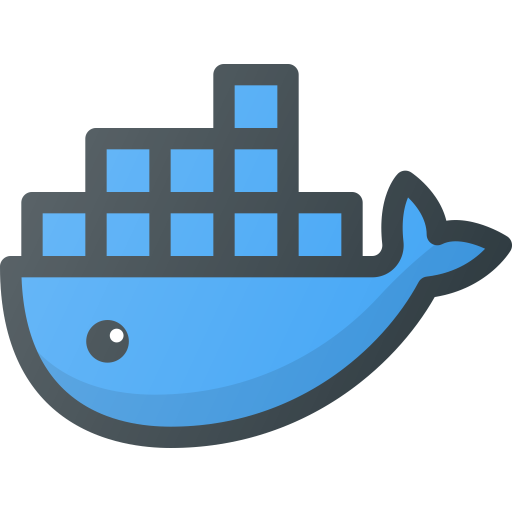
\includegraphics[width=6mm]{../figures/docker_icon.jpg}} ([xshift=-10mm,yshift=-9mm]interior.north west);
    }
}

\newtcblisting{bnflisting}[1][]{%
    #1,
    listing options={
        language=bnf,
        basicstyle=\ttfamily\footnotesize,
        numberstyle=\noncopyable,
        breaklines=true,
        numbers=right,
        showstringspaces=false,
    },
    fonttitle=\ttfamily\small,
    underlay unbroken and first={%
        \path[draw=none] (interior.north west) rectangle node[white]{
\includegraphics[width=5mm]{../figures/bnf_file.png}} ([xshift=-10mm,yshift=-10mm]interior.north west);
    }
}

\newtcblisting{pythonlisting}[1][]{%
    #1,
    listing options={
        language=Python,
        basicstyle=\ttfamily\footnotesize,
        numberstyle=\noncopyable,
        breaklines=true,
        numbers=right,
        showstringspaces=false,
        keywordstyle=\color{blue}\bfseries,
        escapeinside={(*@}{@*)}
    },
    fonttitle=\ttfamily\small,
    underlay unbroken and first={%
        \path[draw=none] (interior.north west) rectangle node[white]{
\includegraphics[width=5mm]{../figures/python_icon.png}} ([xshift=-10mm,yshift=-10mm]interior.north west);
    }
}

\newtcblisting{rpilisting}[1][]{%
    listing options={
        language=BashPrompt,
        basicstyle=\ttfamily\footnotesize,
        numberstyle=\noncopyable,
        tabsize=2,
        inputencoding=utf8,
        #1
    },
    underlay unbroken and first={%
        \path[draw=none] (interior.north west) rectangle node[white]{
\includegraphics[width=8mm]{../figures/raspi_icon.png}} ([xshift=-10mm,yshift=-10mm]interior.north west);
    }
}

\tcbset{
    enhanced jigsaw,
    breakable,
    listing only,
    boxsep=-1pt,
    top=-1pt,
    bottom=-0.5pt,
    right=-0.5pt,
    overlay first={
        \node[black!50] (S) at (frame.south) {\Large\ding{34}};
        \draw[dashed,black!50] (frame.south west) -- (S) -- (frame.south east);
    },
    overlay middle={
        \node[black!50] (S) at (frame.south) {\Large\ding{34}};
        \draw[dashed,black!50] (frame.south west) -- (S) -- (frame.south east);
        \node[black!50] (S) at (frame.north) {\Large\ding{34}};
        \draw[dashed,black!50] (frame.north west) -- (S) -- (frame.north east);
    },
    overlay last={
        \node[black!50] (S) at (frame.north) {\Large\ding{34}};
        \draw[dashed,black!50] (frame.north west) -- (S) -- (frame.north east);
    },
    before={\par\vspace{10pt}},
    after={\par\vspace{\parskip}\noindent}
}

\newcommand*{\inlineimg}[1]{%
    \raisebox{-.3\baselineskip}{%
        \includegraphics[
            height=\baselineskip,
            width=\baselineskip,
            keepaspectratio,
        ]{#1}%
    }%
}

\definecolor{slightgray}{rgb}{0.90, 0.90, 0.90}

\usepackage{soul}
\makeatletter
\def\SOUL@hlpreamble{%
    \setul{}{3.0ex}%
    \let\SOUL@stcolor\SOUL@hlcolor%
    \SOUL@stpreamble%
}
\makeatother

\newcommand{\inline}[1]{%
    \begingroup%
    \sethlcolor{slightgray}%
    \hl{\ttfamily\footnotesize #1}%
    \endgroup
}

\newcommand{\tinline}[1]{%
    \begingroup%
    \sethlcolor{slightgray}%
    \hl{\ttfamily\tiny #1}%
    \endgroup
}


\usepackage{tkz-euclide}

% Downloads Table
\usepackage{pgfplots}
\usepgfplotslibrary{fillbetween}
\usepackage{filecontents}
\usetikzlibrary{pgfplots.dateplot}
\usetikzlibrary{decorations.markings}

%% Packages utiles.
\usepackage{amssymb,subfigure,icomma}
\usepackage[labelfont=bf, width=\linewidth]{caption}

\def\chapterautorefname{Chapter}
\renewcommand{\sectionautorefname}{\S}
\renewcommand{\subsectionautorefname}{\S}
\renewcommand{\figureautorefname}{Fig.}
\renewcommand{\equationautorefname}{Eq.}
\newcommand{\algorithmautorefname}{Algorithm}
\usepackage{hypcap}
\usepackage{bookmark}
\usepackage{amsfonts}

\newtheorem{cor}{\corollaryname}[section]
\newtheorem{deff}[cor]{\definitionname}
\newtheorem{ex}[cor]{\examplename}
\newtheorem{lem}[cor]{\lemmaname}
\newtheorem{prop}[cor]{Proposition}
\newtheorem{rem}[cor]{\remarkname}
\newtheorem{theo}[cor]{\theoremname}

\numberwithin{equation}{section}
\numberwithin{table}{chapter}
\numberwithin{figure}{chapter}

\renewcommand{\baselinestretch}{1.5}

%\AtBeginDocument{\hypersetup{pdfborderstyle={/S/S/W 1}}}
\begin{document}

\version{1}

\title{Programming tools for intelligent systems}

\author{Breandan Considine}

\copyrightyear{2020}

\department{D\'epartement d'informatique et de recherche op\'erationnelle}

\president{Marc Feeley}

\directeur{Liam Paull}

\codirecteur{Michalis Famelis}

\membrejury{Eug\`ene Syriani}

\dateacceptation{La date d'acceptation}

%% Voici les disciplines possibles (voir avec votre directeur):
%% \sujet{statistique},
%% \sujet{mathématiques}, \orientation{mathématiques appliquées},
%% \orientation{mathématiques fondamentales}
%% \orientation{mathématiques de l'ingénieur} et
%% \orientation{mathématiques appliquées}

\sujet{Informatique}

%%
%% Fin des variables à définir. La commande \maketitle créera votre
%% page titre.

\pagenumbering{roman}
\maketitle
\maketitle

% Pour générer la deuxième page titre, il faut appeler à nouveau \maketitle
% Cette page est optionnelle et son inclusion est laissé à la discrétion
% de l'étudiant et du directeur de recherche, ou de tout autre instance
% d'autorité.

%%------------------------------------------------- %
%%              pages iv                            %
%%------------------------------------------------- %
\anglais

%\chapter*{Abstract}
%
%Programming tools are computer programs which help humans program computers. Tools come in all shapes and forms, from editors and compilers to debuggers and profilers. Each of these tools facilitates a core task in the programming workflow which consumes cognitive resources when performed manually. In this thesis, we explore several tools that facilitate the process of building intelligent systems, and which reduce the cognitive effort required to design, develop, test and deploy intelligent software systems. First, we introduce an integrated development environment (IDE) for programming Robot Operating System (ROS) applications, called Hatchery (\autoref{ch:hatchery}). Second, we describe Kotlin$\nabla$, a language and type system for differentiable programming, an emerging paradigm in machine learning (\autoref{ch:kotlingrad}). Third, we propose a new algorithm for automatically testing differentiable programs, drawing inspiration from techniques in adversarial and metamorphic testing (\autoref{ch:difftest}), and demonstrate its empirical efficiency in the regression setting. Fourth, we explore a container infrastructure based on Docker, which enables reproducible deployment of ROS applications on the Duckietown platform (\autoref{ch:ducker}). Finally, we reflect on the current state of programming tools for these applications and speculate what intelligent systems programming might look like in the future (\autoref{ch:conclusion}).
%
%\noindent\textbf{Keywords}: intelligent systems, machine learning, type systems, embedded systems, distributed systems, programming languages, functional programming, differentiable programming, probabilistic programming, programming tools, compilers, automatic differentiation, backpropagation, automated testing, fuzzing, metamorphic testing, property-based testing, generative modeling, static analysis, build automation, continuous integration, virtual machines, ROS, Kotlin, Docker, Duckietown.

\chapter*{Résumé}

\vspace{-40pt} Les outils de programmation sont des programmes informatiques qui aident les humains à programmer des ordinateurs. Les outils sont de toutes formes et tailles, par exemple les éditeurs, les compilateurs, les débogueurs et les profileurs. Chacun de ces outils facilite une tâche principale dans le flux de travail de programmation qui consomme des ressources cognitives lorsqu'il est effectué manuellement. Dans cette thèse, nous explorons plusieurs outils qui facilitent le processus de construction de systèmes intelligents et qui réduisent l'effort cognitif requis pour concevoir, développer, tester et déployer des systèmes logiciels intelligents. Tout d'abord, nous introduisons un environnement de développement intégré (EDI) pour la programmation d'applications Robot Operating System (ROS), appelé Hatchery (\autoref{ch:hatchery}). Deuxièmement, nous décrivons Kotlin$\nabla$, un système de langage et de type pour la programmation différentiable, un paradigme émergent dans l'apprentissage automatique (\autoref{ch:kotlingrad}). Troisièmement, nous proposons un nouvel algorithme pour tester automatiquement les programmes différentiables, en nous inspirant des techniques de tests contradictoires et métamorphiques (\autoref{ch:difftest}), et démontrons son efficacité empirique dans le cadre de la régression. Quatrièmement, nous explorons une infrastructure de conteneurs basée sur Docker, qui permet un déploiement reproductible des applications ROS sur la plate-forme Duckietown (\autoref{ch:ducker}). Enfin, nous réfléchissons à l'état actuel des outils de programmation pour ces applications et spéculons à quoi pourrait ressembler la programmation de systèmes intelligents à l'avenir (\autoref{ch:conclusion}).

\noindent\textbf{Mots-clés}: systèmes intelligents, apprentissage automatique, systèmes de types, systèmes embarqués, systèmes distribués, langages de programmation, programmation fonctionnelle, programmation différentiable, programmation probabiliste, outils de programmation, compilateurs, différentiation automatique, rétropropagation, test automatisé, fuzzing, test métamorphique, test de propriété, modélisation générative, analyse statique, moteur de production, intégration continue, machines virtuelles, ROS, Kotlin, Docker, Duckietown.

\chapter*{Remerciements}

\vspace{-60pt} Je voudrais remercier Gimmey, maman, oncle Mark et papa pour leur amour et leur soutien sans faille. \href{http://hannelita.com/}{Hanneli Tavante} pour m'avoir enseigné la théorie des types et la beauté de la programmation fonctionnelle. \href{https://laverne.edu/directory/person/xiaoyan-liu/}{Xiaoyan Liu} pour avoir semé en moi la graine des mathématiques. Oncle Andy pour avoir arrosé la graine pendant de nombreuses années. Tante Shannon, Adam Devoe et Jacquie Kirrane pour m'avoir encouragé à poursuivre des études supérieures. \href{https://www.cs.rit.edu/~anh/}{Arthur Nunes-Harwitt} pour m'avoir enseigné la différentiation algorithmique il y a longtemps. \href{https://www.sas.rochester.edu/bcs/people/faculty/miller_renee/index.html}{Renee Miller} pour avoir suscité mon intérêt pour la science neuronale. \href{http://blog.locut.us}{Ian Clarke} pour m'avoir montré un nouveau langage intelligent appelé \href{https://kotlinlang.org/}{Kotlin}. \href{https://www.jooq.org/}{Lukas Eder} et \href{https://jonnyzzz.com/}{Eugene Petrenko} pour m'avoir montré la magie des DSL sécurisées et m'avoir donné des conseils sur études supérieures. \href{https://github.com/rusi}{Rusi Hristov} pour sa patience et son mentorat. \href{https://scholar.google.ca/citations?user=PsKlNzUAAAAJ}{Dmitry Serdyuk} et \href{http://kastnerkyle.github.io/}{Kyle Kastner} pour m'avoir présenté à Montréal et me souhaitant la bienvenue dans le groupe de lecture de discours. \href{https://scholar.google.ca/citations?user=-Ss9QGkAAAAJ}{Isabela Albuquerque} et \href{https://scholar.google.ca/citations?user=hkO47vsAAAAJ}{Jo\~ao Monteiro} pour m'avoir montré à quoi ressemblent de bonnes recherches. \href{https://takeitallsource.github.io}{Manfred Diaz} et \href{https://pointersgonewild.com/}{Maxime Chevalier Boisvert} pour l'inspiration, les conversations et les commentaires. \href{http://TurnerComputing.com}{Ryan Turner}, \href{https://saikrishna-1996.github.io}{Saikrishna Gottipati}, \href{https://maivincent.github.io}{Vincent Mai}, \href{https://krrish94.github.io/}{Krishna Murthy}, \href{https://bhairavmehta95.github.io/}{Bhairav ​​Mehta}, \href{https://mila.quebec/fr/person/christos-tsirigotis/}{Christos Tsirigotis}, \href{http://www.solomatov.me/}{Konstantin Solomatov} et \href{https://www.seas.upenn.edu/~ xsi/}{Xujie Si} pour les conversations intéressantes. \href{https://scholar.google.ca/citations?user=bn4xHHIAAAAJ}{Pascal Lamblin}, \href{http://breuleux.net}{Olivier Breleux} et \href{https://scholar.google.ca/citations? user = XE9SDzgAAAAJ}{Bart van Merri\"enboer} et pour éclairer le chemin entre ML et PL. \href{http://christianperone.com}{Christian Perone} pour m'avoir présenté PyTorch, \href{https://research.jetbrains.org/researchers/altavir}{Alexander Nozik}, \href{https://twitter.com/headinthebox}{Erik Meijer}, \href{https://scholar.google.com/citations?user=IcuGXgcAAAAJ}{Kiran Gopinathan}, \href{https://medium.com/@elizarov}{Roman Elizarov}, \href{https://cquic.unm.edu/member/jacob.miller/}{Jacob Miller} et \href{http://www.adampocock.com/}{Adam Pocock} pour leurs commentaires et retours utiles concernant Kotlin$\nabla$. \href{https://diro.umontreal.ca/accueil/}{Celine Begin} à l'Université de Montréal pour avoir aidé un étranger la veille d'un hiver froid en 2017. \href{https://www.iro.umontreal.ca/~monnier/}{Stefan Monnier} pour avoir répondu de manière réfléchie et approfondie à mes courriels errants. \href{https://censi.science/}{Andrea Censi} pour ses conseils et ses encouragements. Enfin et surtout, je tiens à remercier mes brillants conseillers \href{http://liampaull.ca/}{Liam Paull} d'avoir pris une chance sur un échantillon hors distribution, en fournissant de forts gradients et en me donnant beaucoup plus de crédit que je ne le méritais, et \href{https://michalis.famelis.info/}{Michalis Famelis} pour m'avoir enseigné la valeur de la logique intuitionniste, des méthodes formelles et de l'autodiscipline. Merci infiniment!


%%------------------------------------------------- %
%%        page v --- Table de matieres              %
%%------------------------------------------------- %

% Pour un mémoire en anglais, changer pour
% \anglais. Noter qu'il faut une permission
% pour écrire son mémoire en anglais.
% \cleardoublepage termine la page actuel et force TeX
% a poussé les éléments flottant (fig., tables, etc.) sur
% la page (normalement TeX les garde en suspend jusqu'à ce
% qu'il trouve un endroit approprié). Avec l'option <twoside>,
% la commande s'assure que la prochaine page de texte est sur
% le recto, pour l'impression. On l'utilise ici
% pour que TeX sache que la table des matières etc. soit
% sur la page qui suit.
%% TABLE DES MATIÈRES
\cleardoublepage
\pdfbookmark[chapter]{\contentsname}{toc}  % Crée un bouton sur
% la bar de navigation
\tableofcontents
% LISTE DES TABLES
\cleardoublepage
%\phantomsection  % Crée une section invisible (utile pour les hyperliens)
\listoftables
% LISTE DES FIGURES
\cleardoublepage
%\phantomsection
\listoffigures

\NoChapterPageNumber
\cleardoublepage
\pagenumbering{arabic}

\chapter{Introduction}\label{ch:introduction}

\setlength{\epigraphwidth}{0.85\textwidth}
\epigraph{``Il y a une course entre la complexité croissante des systèmes que nous construisons et notre capacité à développer des outils intellectuels pour comprendre leur complexité. Si la course est gagnée par nos outils, les systèmes deviendront finalement plus faciles à utiliser et plus fiables. Sinon, ils continueront à être plus difficiles à utiliser et moins fiables pour tous, sauf pour un ensemble relativement restreint de tâches communes. Étant donné la difficulté de la réflexion, si ces outils intellectuels doivent réussir, ils devront remplacer la pensée par le calcul.''}{\begin{flushright}--Leslie \citet{lamport2002discussion}, \href{https://www.microsoft.com/en-us/research/uploads/prod/2016/12/A-Discussion-With-Leslie-Lamport.pdf}{\textit{Une discussion avec Leslie Lamport}}\end{flushright}}

La complexité du calcul est une telle préoccupation en informatique qu'une grande partie du domaine est consacrée à sa compréhension à travers la lentille de l'analyse des fonctions et de la théorie de l'information. Dans le domaine du génie logiciel, les chercheurs s'intéressent principalement à la complexité de la construction des logiciels, c'est-à-dire la manifestation numérique des algorithmes sur le matériel physique. Un type de complexité logicielle est l'effort cognitif requis pour comprendre un programme. Bien que les logiciels d'aujourd'hui deviennent rapidement plus intelligents, ils ne montrent que peu de signes de devenir plus intelligibles. De meilleurs outils sont nécessaires pour gérer la complexité des systèmes logiciels de construction.

\textit{L'objectif de cette thèse est de développer des méthodes qui réduisent l'effort cognitif nécessaire pour construire des systèmes intelligents, en utilisant des outils de développement, des abstractions de langage de programmation, des tests automatisés et la technologie de virtualisation.}

D'une manière générale, les systèmes intelligents diffèrent des systèmes logiciels ordinaires en ce qu'ils permettent aux machines de détecter des modèles, d'exécuter des tâches et de résoudre des problèmes qu'elles ne sont pas explicitement programmées pour résoudre et que les experts humains étaient auparavant incapables de résoudre en codant en dur des règles explicites. Généralement, ces systèmes sont capables de:\\
%
\begin{enumerate}
\item apprendre des règles généralisables en traitant de grandes quantités de données
\item régler un grand nombre de paramètres libres (des milliers à des milliards)
\item surpasse les humains bien formés dans des tâches spécifiques à un domaine
\end{enumerate}
%
Si l'idée de systèmes intelligents existe depuis des décennies, trois évolutions essentielles ont fait le succès des systèmes intelligents modernes. Premièrement, la puissance de traitement des ordinateurs est devenue plus rapide, moins chère et beaucoup plus facilement disponible. De même, la numérisation de nouveaux ensembles de données a rendu disponibles de vastes quantités d'informations et les coûts de stockage des données ont chuté de façon spectaculaire. (Une clé USB de \$5 a aujourd'hui une capacité de stockage 200 fois supérieure à celle d'un disque dur IBM de 5 MB de 2,000 livres, loué pour \$3,000 par mois en 1956). Plus important encore, a été le développement d'algorithmes d'apprentissage plus efficaces.

Ces dernières années, l'informatique et le génie logiciel ont fait des progrès considérables dans la construction et le déploiement de systèmes intelligents. Presque tous les ordinateurs mobiles du monde sont capables de détecter des objets dans des images, d'effectuer des traductions de la parole au texte et des traductions de langue. Ces percées sont le résultat direct des progrès fondamentaux réalisés dans le domaine des réseaux neuronaux et de l'apprentissage de la représentation. L'adoption de pratiques collaboratives à code source ouvert, dont la communauté du génie logiciel a été la pionnière, a également été la clé du succès des systèmes intelligents modernes. Les ingénieurs en logiciel ont développé des bibliothèques de différenciation automatique comme Theano~\citep{bergstra2010theano}, Torch~\citep{collobert2002torch} et Caffe~\citep{jia2014caffe}, et ont construit de nombreux simulateurs populaires pour l'apprentissage du renforcement. La facilité d'utilisation et la disponibilité de ces outils ont été cruciales pour démocratiser les techniques d'apprentissage approfondi.

Les systèmes intelligents sont largement déployés dans des environnements virtuels comme la science des données et les services en ligne. Mais même avec l'énorme succès des algorithmes d'apprentissage automatique dans des domaines entièrement observables comme la reconnaissance d'images et le traitement de la parole, les systèmes intelligents n'ont pas encore été largement adoptés en robotique (au moment de la rédaction de cette thèse). Ce dilemme peut être partiellement attribué à divers problèmes théoriques tels que l'adaptation au domaine et l'apprentissage par transfert. Pourtant, grâce aux capacités éprouvées des algorithmes d'apprentissage modernes, à l'augmentation exponentielle de la puissance de traitement et aux efforts déployés depuis des décennies pour construire des agents intelligents physiquement incorporés, nous devrions avoir plus de progrès à montrer. Pourquoi cet objectif a-t-il échappé aux chercheurs pendant si longtemps ? L'une des raisons, nous le supposons, est le manque d'outils de programmation et d'abstractions pour concevoir, développer, déployer et évaluer les systèmes intelligents. En pratique, ces activités consomment une grande quantité d'efforts cognitifs sans le bon ensemble d'outils et d'abstractions.

Dans le domaine du génie logiciel traditionnel, le modèle Waterfall est un modèle classique de développement de logiciels comprenant différentes étapes~\citep{royce1987managing}. Nous proposons des contributions à quatre étapes: Premièrement, nous faisons la démonstration d'un environnement de développement intégré pour les logiciels de robotique \textit{conception} (\autoref{ch:hatchery}). Ensuite, nous montrons un langage spécifique à un domaine et sans danger pour les programmes différenciables de \textit{implémentation}, un paradigme émergent dans l'apprentissage profond (\autoref{ch:kotlingrad}). Pour \textit{vérifier} cette application, nous utilisons un ensemble de techniques empruntées aux tests basés sur les propriétés~\citep{fink1997property} et à l'apprentissage contradictoire~\citep{lowd2005adversarial} (\autoref{ch:difftest}). Les conteneurs Docker~\citep{merkel2014docker} sont utilisés pour automatiser le \textit{maintenance} d'applications robotiques reproductibles sur des plateformes matérielles hétérogènes (\autoref{ch:ducker}). Enfin, nous présentons quelques remarques de conclusion et les enseignements tirés de la construction de ces outils (\autoref{ch:conclusion}).

%\begin{figure}[H]
%\center
%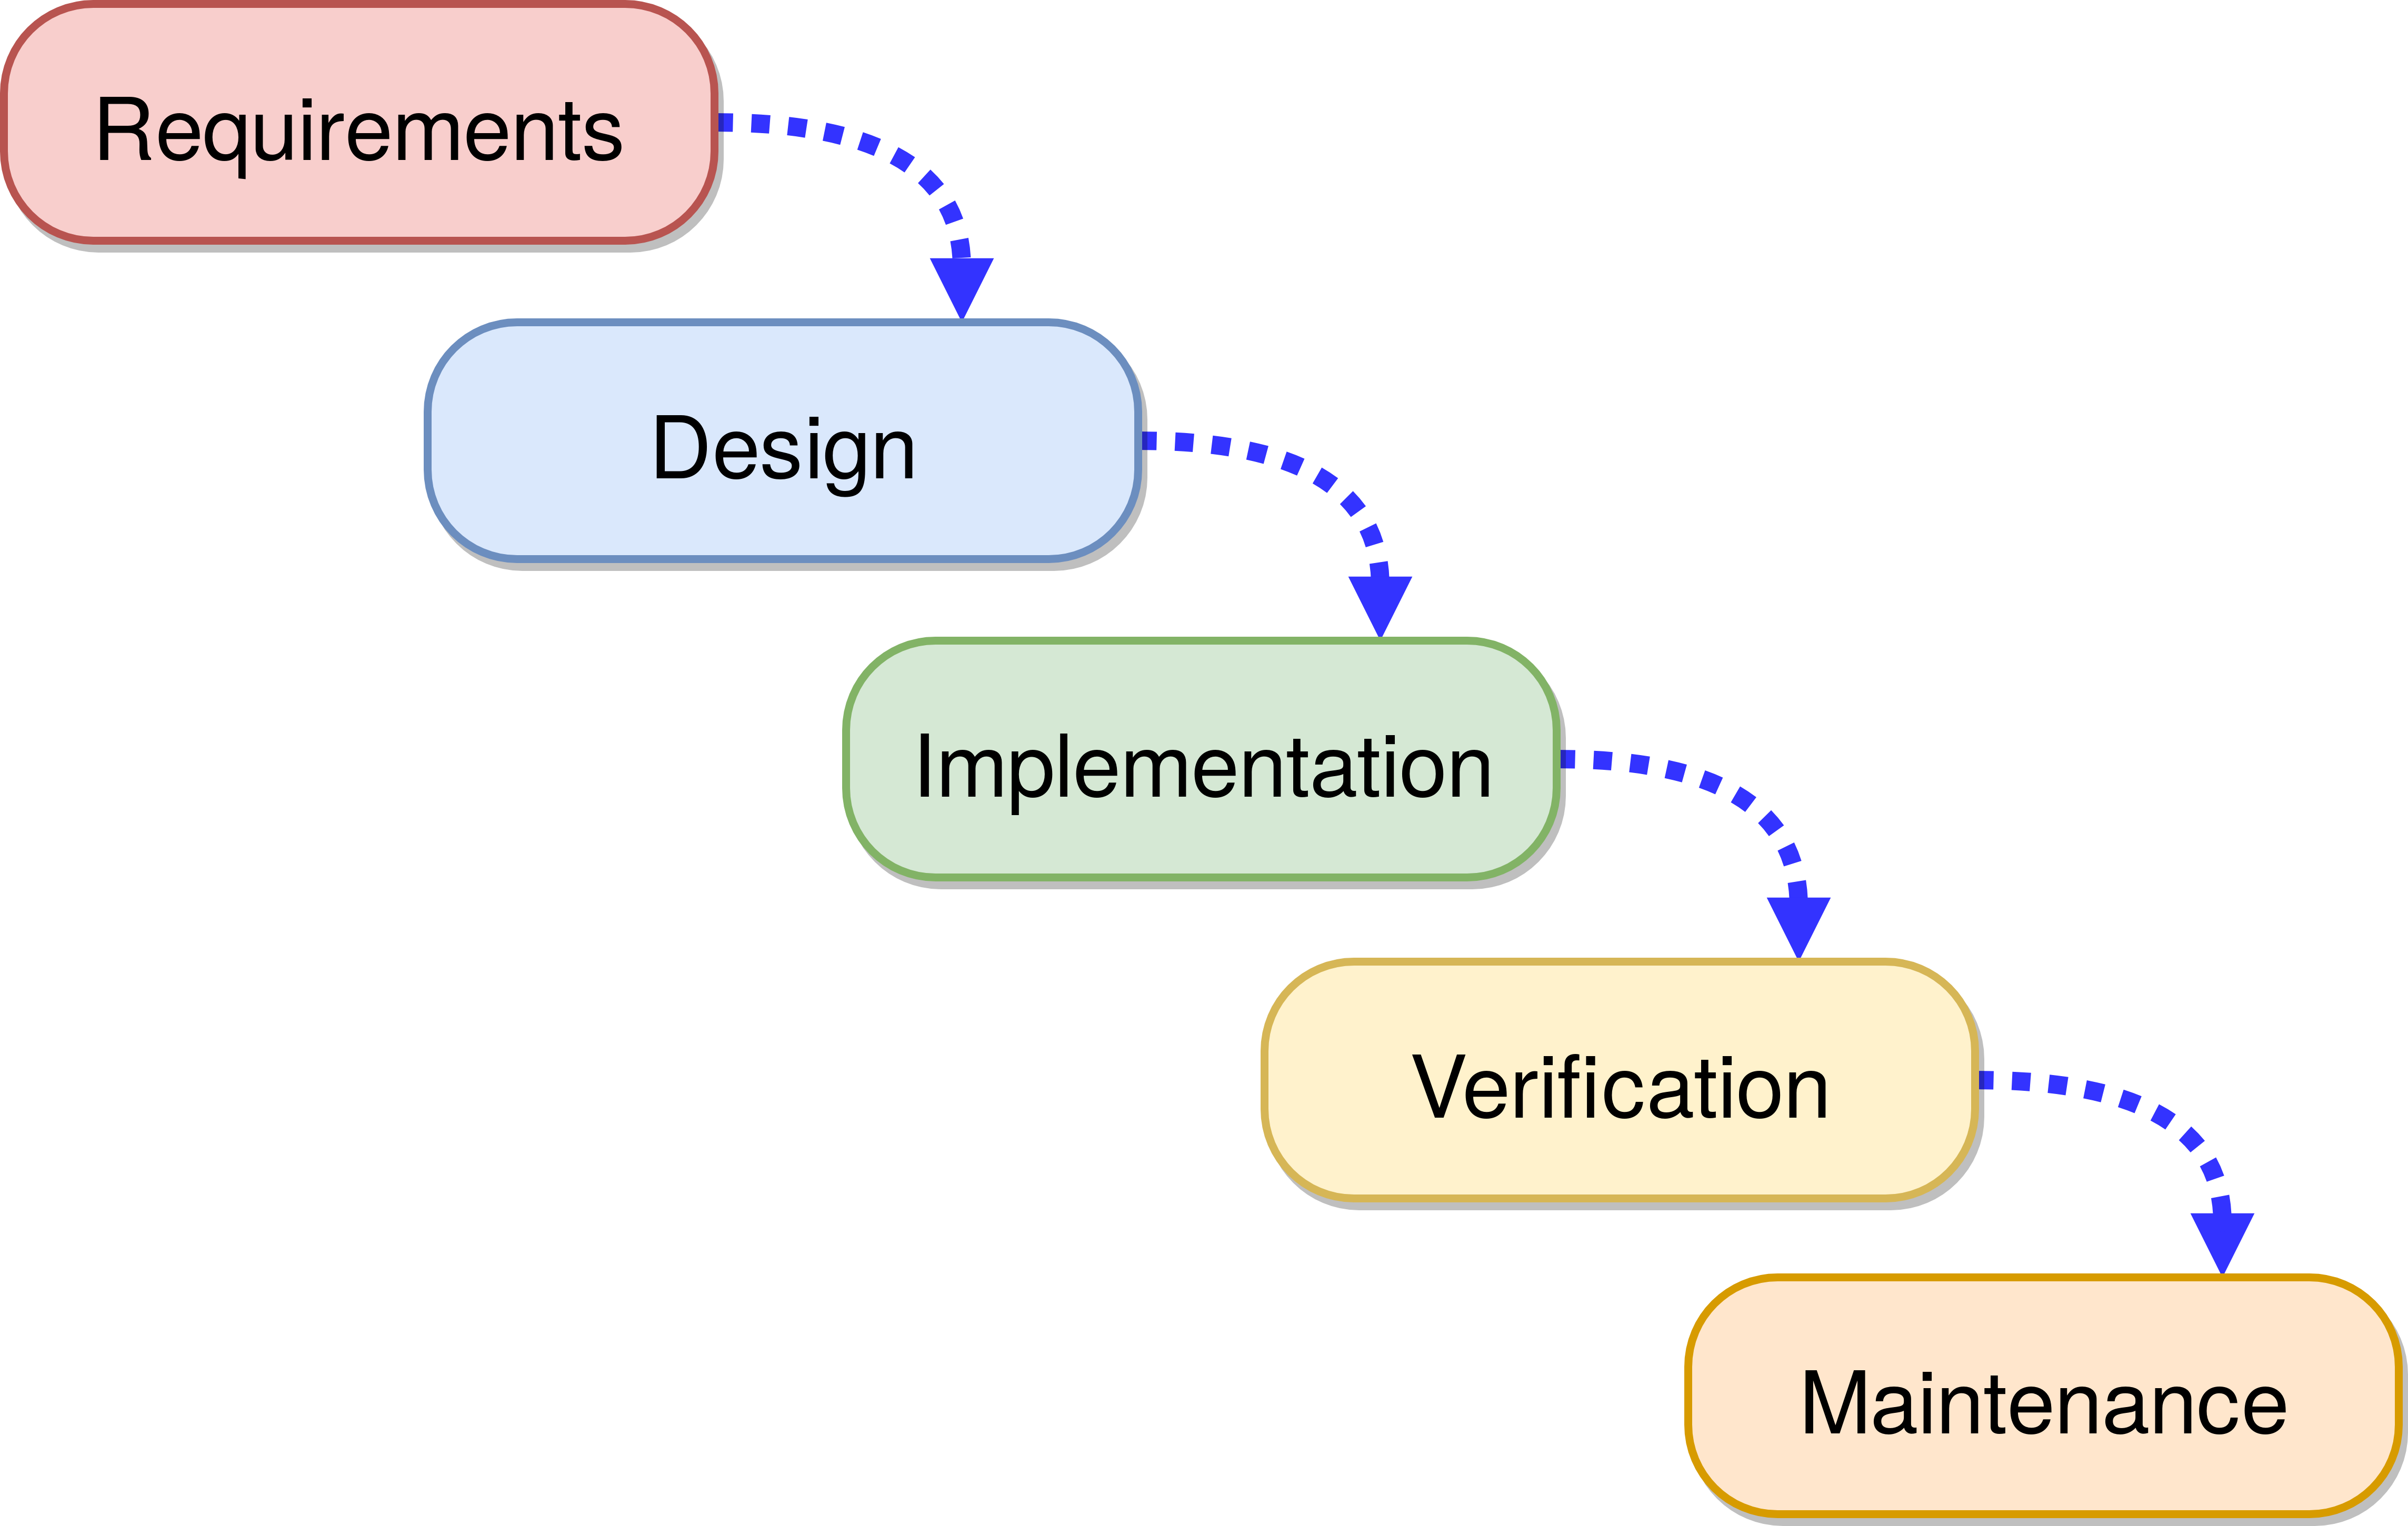
\includegraphics[width=0.70\textwidth]{../figures/waterfall_diagram.png}
%\caption{Le modèle original de cascade de Royce décrit le processus de développement du logiciel. Nous l'utilisons pour guider notre discussion et encadrer nos contributions à l'intérieur de ce modèle.
%\label{fig:waterfall_model}}
%\end{figure}

\section{Conception: Outils de programmation pour la robotique}

Les systèmes logiciels d'aujourd'hui sont des entités profondément complexes. L'époque où un programmeur solitaire, même très compétent, pouvait assurer seul la maintenance d'un grand système logiciel est révolue. Pour mettre efficacement à l'échelle les systèmes logiciels modernes, les programmeurs doivent mettre en commun leur capacité mentale pour former un graphe de connaissances. Les projets logiciels qui reposent sur un petit nombre de responsables ont tendance à disparaître en raison de ce que l'on appelle le "facteur \textit{bus}~\citep{cosentino2015assessing} -- de grandes parties du graphe de connaissances sont enfermées dans la tête de quelqu'un. Les projets logiciels réussis apprennent à distribuer ce graphe et à établir des connexions avec le monde extérieur. Le graphe de connaissances qui s'accumule autour d'un projet logiciel contient des faits, mais aussi des flux de travail pour la programmation, le débogage et la livraison -- des chemins communs à travers le labyrinthe du développement logiciel~\citep{naur1985programming}. Les composants de ce graphique peuvent être engagés à l'écriture, mais la documentation prend du temps et devient périmée avec le temps. Ce qu'il faut, c'est un système qui offre les avantages de la documentation sans les inconvénients de la maintenance.

Le développement de systèmes logiciels comporte un deuxième élément, le graphe social. Le graphe social d'un projet logiciel réussi contient les concepteurs de produits, les gestionnaires et les ingénieurs logiciels qui travaillent de concert pour construire un logiciel bien conçu, cohésif et très performant. Cela implique parfois de réviser la spécification pour tenir compte des défis techniques, ou de réécrire le code source pour supprimer la dette technique. La conception de logiciels est un processus d'optimisation à objectifs multiples et nécessite des collaborateurs ayant un large éventail de compétences et un ensemble d'objectifs communs. Pour produire un logiciel qui se rapproche des critères de ses intervenants, les développeurs sont invités à fournir des prototypes rapides et à intégrer en permanence les commentaires des utilisateurs. Pourtant, les systèmes logiciels d'aujourd'hui sont plus grands et plus compliqués que jamais. Il est donc essentiel de trouver des moyens de collaborer plus efficacement pour construire des systèmes plus intelligents.

Examinons tout d'abord le processus mécanique d'écriture de logiciels à l'aide d'un clavier.

Les environnements de développement intégrés (EDI) peuvent aider les développeurs à créer des applications logicielles complexes en automatisant certaines tâches de programmation répétitives. Par exemple, les EDI effectuent des analyses et des inspections statiques pour détecter rapidement les bogues. Ils permettent de compléter, de remanier et de naviguer dans le code source, et ils automatisent le processus de construction, d'exécution et de débogage des programmes. Bien que ces tâches puissent sembler insignifiantes, leur automatisation promet d'accroître la productivité des développeurs en leur permettant de fournir un retour d'information plus tôt, de détecter les erreurs d'écriture et de libérer des ressources mentales qui pourront être utilisées ailleurs. Plutôt que d'être obligés de se concentrer sur la structure et l'organisation du texte, si les développeurs sont capables de manipuler le code à un niveau sémantique, ils seront beaucoup plus heureux et plus productifs. De plus, en automatisant les tâches mécaniques dans le développement de logiciels, ces outils libèrent l'attention vers l'activité fondamentale de l'écriture et de la compréhension des programmes.

Mais que font réellement les EDI? Ils guident les développeurs à travers le graphe de connaissances d'un projet logiciel. Pensez à ce qu'un nouveau développeur doit apprendre pour se mettre à niveau: en plus d'apprendre le langage, les développeurs doivent apprendre à utiliser des bibliothèques et des cadres (sans doute des langages à part entière). Ils doivent se familiariser avec les outils en ligne de commande pour le développement de logiciels, des outils de construction au contrôle de version et à l'intégration continue. Ils doivent se familiariser avec l'écosystème du logiciel, les styles de programmation, les conventions et les flux de développement. Et ils doivent apprendre à collaborer au sein d'une équipe distribuée de développeurs. En automatisant les tâches courantes dans un environnement de programmation interactif et en rendant explicite la connectivité des graphes grâce au balisage des documents~\citep{goldfarb1981generalized} et à l'édition de projets~\citep{voelter2014towards}, un EDI bien conçu est un outil de traversée de graphes. Il n'est pas surprenant que les EDI soient en fait des bases de données de graphes.

Sous certains aspects, le développement de systèmes intelligents n'est pas différent du génie logiciel classique. Les mêmes principes et meilleures pratiques qui guident le génie logiciel sont également applicables aux systèmes intelligents. Et les mêmes activités, de la conception à la maintenance, continueront à jouer un rôle important dans la construction de systèmes intelligents. Mais à d'autres égards, les outils de programmation génériques utilisés pour développer des logiciels traditionnels nécessiteront des adaptations spécifiques à chaque domaine pour que les systèmes d'apprentissage deviennent des citoyens de premier ordre dans la prochaine génération de logiciels intelligents, notamment dans le cas du développement de la robotique.

Dans ce but, nous avons développé un EDI pour le \href{https://www.ros.org/}{Système d'exploitation des robots} (ROS) appelé \href{https://github.com/duckietown/hatchery}{Hatchery}. Il prend en charge un certain nombre de flux de travail communs pour le développement des ROS, tels que la création de nœuds ROS, l'intégration du simulateur Gazebo, la prise en charge du débogage à distance, l'analyse statique, l'autocomplétion et le refactoring. Dans \autoref{ch:hatchery} nous discutons de la mise en œuvre de ces fonctionnalités et de certains des défis liés à la prise en charge du langage, aux outils de programmation et à l'intégration avec le middleware ROS. Nous soutenons que ces outils réduisent la complexité cognitive de la construction d'applications ROS en adoptant des conventions de codage explicites, en annotant le texte non structuré et en automatisant les tâches de développement répétitives.

\section{Implémentation: Programmation différenciée par type}

Aux premiers temps de l'apprentissage machine, on croyait généralement que l'intelligence à l'échelle humaine émergerait d'une logique de premier ordre suffisamment descriptive. En accumulant une base de données de faits et de leurs relations, les chercheurs pensaient pouvoir utiliser un raisonnement symbolique pour contourner l'apprentissage. Cette approche fondée sur des règles a dominé une grande partie des premières recherches sur l'intelligence artificielle et des efforts considérables ont été consacrés à la création d'ontologies propres à chaque domaine pour saisir les connaissances humaines. Malgré les meilleurs efforts des roboticiens, des ingénieurs en traitement du signal et des chercheurs en langage naturel, les \textit{systèmes experts} n'ont pas pu s'adapter aux applications du monde réel, ce qui a provoqué une grande désillusion dans la recherche sur l'intelligence artificielle pendant plusieurs décennies. Alors que les informaticiens ont sous-estimé la difficulté de l'\textit{apprentissage}, les systèmes experts ont excellé dans des domaines où les systèmes actuels d'apprentissage machine ont du mal à s'adapter, comme le raisonnement classique et l'interprétabilité, et il y a de plus en plus de preuves qui suggèrent que beaucoup de ces idées étaient simplement en avance sur leur temps. Dans notre travail, nous nous inspirons de certains travaux antérieurs sur le raisonnement symbolique~\citep{dwyer1948symbolic, glushkov1971analitik}, les systèmes de types~\citep{lof1973intuitionistic,jay1996shape} et la programmation fonctionnelle~\citep{mccarthy1960recursive, abelson1996structure}.

Ce qui a finalement été montré à l'échelle, c'est l'idée de l'apprentissage connexionniste. En imbriquant des approximateurs de fonctions aléatoires, appelés perceptrons, et en mettant à jour les paramètres libres à l'aide de la rétropropagation~\citep{werbos1990backpropagation, rumelhart1988learning}, le système résultant est capable d'apprendre une quantité surprenante de comportements intelligents. L'approche, appelée réseaux neuronaux artificiels (ANN), remonte au milieu du 20ème siècle~\citep{ivakhnenko1965cybernetic, rosenblatt1958perceptron}, mais n'a été pleinement réalisée in silico qu'après la généralisation de l'informatique bon marché et des grands ensembles de données~\citep{lecun2015deep}. En théorie, une seule couche d'imbrication est capable d'approcher toute fonction différentiable continue~\citep{hornik1989multilayer}, mais en pratique, l'apprentissage nécessite de composer de nombreux approximateurs de ce type de manière profondément imbriquée, d'où le terme, \textit{deep neural networks} (DNNs). L'importance de la profondeur a été soupçonnée pendant de nombreuses années, mais l'algorithme de rétropropagation original avait des difficultés à former les DNN en raison du problème du gradient de disparition~\citep{bengio1994learning}. La résolution de ce problème a nécessité un certain nombre d'adaptations et de nombreuses années pour être entièrement débogué. Ce n'est que vers 2013 que l'apprentissage approfondi est devenu compétitif par rapport aux experts humains dans des domaines spécifiques.

Bien qu'il ait fallu une recherche fondamentale en matière d'apprentissage approfondi pour réaliser le plan connexionniste, le succès de l'apprentissage approfondi moderne peut être en partie attribué aux outils logiciels de calcul des dérivés mathématiques, une étape clé de l'algorithme de rétropropagation. Bien qu'il n'ait pas encore été établi si et comment les dérivés peuvent être calculés dans les circuits biologiques, les dérivés sont essentiels pour la formation des ANN. Pendant de nombreuses années, la forme symbolique de ces dérivés a été dérivée analytiquement lors du prototypage d'une nouvelle architecture de réseau neuronal, un processus fastidieux et sujet aux erreurs. Il existe un algorithme bien connu dans la communauté du calcul scientifique qui remonte aux années 1970, appelé \textit{différenciation automatique} (AD)~\citep{linnainmaa1970representation, griewank1989automatic}, qui est capable de calculer des dérivés pour des fonctions différentiables arbitraires. Mais étonnamment, ce n'est que beaucoup plus tard, après le développement de Theano~\citep{bergstra2010theano}, que l'AD a été largement adopté par la communauté de l'apprentissage machine. Cette bibliothèque a considérablement accéléré le rythme de la recherche sur l'apprentissage profond et a stimulé le développement d'autres cadres AD comme TensorFlow~\citep{abadi2016tensorflow} et PyTorch~\citep{paszke2019pytorch}.

Les systèmes intelligents conçus doivent réfléchir attentivement aux langages et aux abstractions. Si les développeurs doivent mettre en œuvre la rétropropagation à la main, ils auront peu de temps pour réfléchir aux caractéristiques de haut niveau de ces systèmes. De même, si les abstractions de programmation sont trop spécifiques, de petites variations nécessiteront une réimplémentation coûteuse. Cela n'est pas différent du génie logiciel traditionnel - en tant qu'ingénieurs, nous devons choisir les bonnes abstractions pour la tâche à accomplir. Trop bas niveau et la conception se perd dans les détails -- trop abstrait et les détails se perdent complètement. Avec un apprentissage approfondi, la nécessité de choisir de bonnes abstractions est encore plus importante, car la relation entre le code source et le comportement est déjà difficile à déboguer, en raison de la complexité des réseaux de neurones et de la programmation des tableaux. Une composante de cette complexité se trouve dans le système de types.

La plupart des cadres AD existants pour l'apprentissage machine sont écrits dans des langages à typage dynamique comme Python, Lua et JavaScript, avec quelques premières implémentations, notamment des projets comme \href{http://deeplearning.net/software/theano/}{Theano}~\citep{bergstra2010theano}, \href{http://torch.ch/}{Torch}~\citep{collobert2002torch} et \href{https://caffe.berkeleyvision.org/}{Caffe}~\citep{jia2014caffe}. Des idées similaires sont apparues dans des langages fonctionnels à caractères statiques, tels que Java (\href{https://github.com/uniker9/JAutoDiff}{JAutoDiff}~\citep{nureki2012jautodiff}, \href{https://deeplearning4j.org/}{DL4J}~\citep{team2016dl4j}, \href{https://github.com/Hipparchus-Math/hipparchus}{Hipparchus}~\citep{andrea2016automatic}), Scala (\href{https://tongfei. me/nexus/}{Nexus}~\citep{chen2017typesafe}), F\# (\href{http://diffsharp.github.io/DiffSharp/}{DiffSharp}~\citep{baydin2015diffsharp}), \href{https://www. tensorflow.org/swift}{Swift}~\citep{lattner2018tensorflow}, Haskell (\href{https://github.com/leopiney/tensor-safe}{TensorSafe}~\citep{pineyro2019structure}) et al, mais peu d'entre eux sont capables de vérifier la forme des tableaux multidimensionnels dans leur système de types, et ceux qui le font sont implémentés dans des langages expérimentaux avec des types dépendants. Dans notre travail, nous démontrons la viabilité de la vérification de type dans un langage largement utilisé. Cela garantit que les programmes sur les matrices, s'ils se compilent, ont la forme correcte et peuvent être évalués numériquement au moment de l'exécution.

\href{https://github.com/breandan/kotlingrad/}{Kotlin$\nabla$} est un langage dédié interne (eDSL) pour la programmation différenciable dans un langage appelé \href{https://kotlinlang.org}{Kotlin}, un langage de programmation à caractères statiques prenant en charge la programmation asynchrone et la compilation multi-plateforme. Dans Kotlin$\nabla$ (\autoref{ch:kotlingrad}), nous décrivons une implémentation algébrique de la différenciation automatique avec des opérations de tenseur de type sécurisé. Notre approche diffère de la plupart des cadres AD existants dans la mesure où Kotlin$\mathbf{\nabla}$ est la première bibliothèque de type sécurisé AD à entièrement compatible avec le système de type Java, ne nécessitant aucune métaprogrammation, réflexion ou intervention du compilateur pour être utilisée.

\section{Vérification: Tester les systèmes intelligents}

La plupart des phénomènes naturels, en particulier ceux liés à la vision, à la planification et à la locomotion, sont des créatures de grande dimension. Richard Bellman a célèbremment appelé ce problème la "fléau de la dimensionnalité". Notre univers physique est peuplé de problèmes simples à poser, mais apparemment impossibles à résoudre en son sein. Claude Shannon, un contemporain de Bellman, a calculé que le nombre de parties d'échecs uniques dépassait $10^{120}$, soit plus que le nombre d'atomes dans l'univers d'environ quarante ordres de grandeur~\citep{shannon1950chess}. À l'époque, on pensait que de tels problèmes seraient insurmontables sans percées fondamentales dans les algorithmes et les machines informatiques. En effet, si Bellman ou Shannon n'ont pas vécu pour voir le jour, il n'a fallu qu'un demi-siècle de progrès en informatique~\citep{campbell2002deep} avant que des solutions à des problèmes du même ordre de complexité, découverts pour la première fois lors de l'explosion cambrienne il y a 541 millions d'années, soient mises en œuvre avec une marge concurrentielle sur les ordinateurs modernes~\citep{pratt2015cambrian}.

Alors que l'informatique a fait d'énormes progrès dans la résolution des cas les plus courants, le fléau de la dimensionnalité de Bellman hante toujours la longue queue de l'apprentissage machine, en particulier des distributions très dispersées. Comme la dimensionnalité de nombreuses fonctions du monde réel que nous voudrions approcher est d'une ampleur insurmontable, il est difficile de vérifier le comportement d'une solution candidate dans tous les régimes, en particulier dans des contextes où les échecs sont rares mais catastrophiques. Selon certaines études, les conducteurs humains comptent en moyenne 1,09 décès par cent millions de miles~\citep{kalra2016driving}. Un nouveau logiciel pour un véhicule autonome devrait accumuler 8,8 milliards de miles de conduite afin d'approcher le taux de mortalité d'un conducteur humain à 20\% près avec un intervalle de confiance de 95\%. Le déploiement d'un tel système dans le monde réel serait problématique sur le plan logistique, sans parler de l'éthique.

D'un point de vue réaliste, les systèmes intelligents ont besoin de meilleurs moyens de mettre en pratique leurs compétences et de sonder l'efficacité d'une solution candidate dans le cadre d'un budget de calcul limité, sans nuire aux humains dans le processus. L'objectif de ces tests est de mettre en évidence les erreurs, mais aussi, en fin de compte, de fournir un retour d'information au système. Dans le domaine du génie logiciel, le véritable système testé est l'écosystème des humains et des machines qui se fournissent mutuellement des moyens de subsistance. Le succès de cet arrangement dépend d'un mécanisme de test externe pour appliquer une barre de rigueur minimale, généralement une forme de test matériel ou humain en boucle. Si le mécanisme de test n'est pas opposé d'une manière ou d'une autre au système testé, un système intelligent peut se tromper, ce qui n'est ni dans l'intérêt du système ni dans celui de ses utilisateurs.

Plus largement, nous pouvons considérer la vérification de type (\autoref{ch:kotlingrad}) et les tests automatisés (\autoref{ch:difftest}) comme faisant partie d'un ensemble d'outils plus large pour la vérification et la validation des logiciels. Plus les anomalies sont détectées rapidement, plus elles sont faciles à corriger et plus les systèmes autonomes peuvent devenir sûrs. Les précédentes approches de tests automatisés ont nécessité une expertise de domaine considérable pour être déployées avec succès, mais les progrès récents en matière de tests métamorphiques~\citep{chen1998metamorphic} et d'apprentissage autosurveillé~\citep{lieb2005adaptive} ont montré des applications dans des domaines de plus en plus généraux~\citep{zhang2020testing}. Dans ce but, nous proposons dans \autoref{ch:difftest} un nouvel algorithme inspiré des tests basés sur les propriétés et de l'apprentissage contradictoire qui améliore empiriquement l'efficacité des données et nécessite beaucoup moins d'expertise de domaine pour être mis en œuvre que les méthodes basées sur les propriétés natives.

\section{Maintenance: Outils pour une robotique reproductible}

L'un des défis de la construction de systèmes intelligents et de la programmation en général, est le problème de la reproductibilité. La reproductibilité des logiciels comporte plusieurs aspects difficiles, notamment la compatibilité matérielle, les systèmes d'exploitation, les systèmes de fichiers, les systèmes de construction et le déterminisme d'exécution. Alors que l'écriture de programmes et leur introduction directe dans un ordinateur a pu être une pratique courante par le passé, le code source actuel est bien trop éloigné de sa réalisation mécanique pour être exécuté de manière significative de manière isolée. Les programmes manuscrits d'aujourd'hui sont comme les schémas d'un feu de circulation - construits à l'intérieur d'une usine, et qui nécessitent une infrastructure, des voitures et des règles de circulation digne d'une ville pour remplir leur fonction. Comme les feux de signalisation, le code source n'existe pas dans le vide -- construit par des compilateurs, interprété par des machines virtuelles, exécuté à l'intérieur d'un système d'exploitation, et qui suit un protocole de communication spécifique -- les programmes sont essentiellement des abstractions dénuées de sens en dehors de ce contexte.

Comme le veut tout bon schéma, une grande partie des informations nécessaires à la construction d'un programme est divisée en couches d'abstraction. La plupart des instructions de bas niveau exécutées par un ordinateur pendant l'exécution d'un programme n'ont pas été écrites ni destinées à être lues par le programmeur et ont depuis été automatisées et oubliées. Dans un langage de programmation moderne comme Java, C\# ou Python, l'ensemble des informations nécessaires à l'exécution d'un programme simple se chiffre souvent en billions de bits. Une partie de ces données concerne le logiciel de construction et d'exécution des programmes, y compris le système de construction, les dépendances logicielles et les outils de développement. Une partie des données concerne le système d'exploitation, les microprogrammes, les pilotes et les logiciels intégrés. Pour la plupart des programmes, tels que ceux que l'on trouve dans un dépôt GitHub typique, une petite partie des informations correspond au code source lui-même.

L'apprentissage machine appliqué partage bon nombre des mêmes défis pratiques que le développement traditionnel de logiciels, avec le code source, la gestion des versions et des dépendances. Le processus actuel de formation d'un modèle d'apprentissage approfondi peut être considéré comme une étape de compilation particulièrement longue, mais il en diffère sensiblement dans la mesure où le code source est un langage de haut niveau qui ne décrit pas directement le calcul effectué, mais est une sorte de méta-programme. Le premier méta-programme décrit la connectivité d'un grand graphe dirigé (c'est-à-dire un graphe de calcul ou un modèle graphique probabiliste), paramétré par des poids et des biais. Le réglage de ces paramètres est un autre méta-programme, qui décrit la séquence d'opérations nécessaires pour se rapprocher d'un programme auquel nous n'avons pas accès, à l'exception de quelques exemples d'entrées-sorties. Les techniques émergentes en matière de méta-apprentissage et d'optimisation des hyper-paramètres (par exemple recherche d'architecture différentiable~\citep{liu2018darts}) ajoutent encore d'autres couches de méta-programmation à cette pile, en effectuant des recherches dans l'espace des graphes dirigés eux-mêmes.

Les fabricants de matériel informatique ont mis au point divers accélérateurs spécialisés pour former et exécuter rapidement ces programmes. Mais contrairement à la plupart des programmes, l'apprentissage profond est un modèle de calcul beaucoup plus simple -- tant qu'un ordinateur peut additionner et multiplier, il a la capacité de faire fonctionner un réseau neuronal profond. Cependant, en raison de la variété des plates-formes matérielles qui existent et des changements de logiciels qui y sont associés, la reproduction des modèles d'apprentissage profond peut être laborieusement difficile sur du nouveau matériel, même avec le même code source et les mêmes dépendances. De nombreux formats de graphes, ou \textit{représentations intermédiaires} (IR) dans le langage des compilateurs, promettent la portabilité du matériel mais si les développeurs ne sont pas prudents, leurs modèles peuvent ne pas converger pendant la formation ou peuvent produire des résultats différents sur des matériels différents. Pour compliquer le problème, les IR sont produits par des vendeurs concurrents, qui vendent des puces concurrentes avec des normes incompatibles (par exemple MLIR~\citep{mlir}, ONNX~\citep{bai2019}, nGraph~\citep{cyphers2018intel}, Glow~\citep{rotem2018glow}, TVM~\citep{tvm2018} et al.) Si certains ont essayé d'exploiter les compilateurs existants tels que GHC~\citep{elliott2018simple} ou DLVM/LLVM~\citep{wei2017dlvm}, il y a peu de signes d'une interopérabilité plus large au moment de la rédaction de cette thèse.

En fin de compte, les chercheurs doivent reproduire les travaux d'autres chercheurs, mais l'effort mental de réimplanter des abstractions de base peut entraver le progrès scientifique. Les outils qui facilitent la reproductibilité et le développement progressif des logiciels sont essentiels. Heureusement, c'est le même problème qui préoccupe l'industrie du logiciel depuis de nombreuses années et qui a produit de nombreux logiciels gestion de versions (VCS). Mais le VCS seul est insuffisant, car ces outils sont principalement destinés à stocker du texte. Les représentations basées sur le texte sont temporairement stables, mais lorsque les dépendances sont mises à jour et reconstruites, des détails importants sur l'environnement de développement original peuvent être égarés. Pour reproduire un programme dans son intégralité, il faut un instantané de toutes les informations numériques disponibles pendant l'exécution, et idéalement, l'ordinateur physique lui-même. En l'absence d'un instantané complet, il est hautement souhaitable de disposer d'un ensemble minimal de dépendances et d'une réplique quasi physique. Toute variabilité dans le graphique des dépendances physiques ou numériques peut être une source de divergences qui nécessite du temps et de l'énergie pour les isoler ultérieurement.

Afin d'atténuer les effets de la variabilité des logiciels et d'aider au développement de systèmes intelligents sur des plateformes hétérogènes, nous utilisons un outil de développement appelé \href{https://www.docker.com}{Docker}, qui fait partie d'un ensemble d'outils d'automatisation de la construction et des opérations de développement que nous appellerons \textit{container infrastructure}. Docker permet aux développeurs de figer une application logicielle et son environnement hôte, ce qui permet aux développeurs (par exemple en utilisant un environnement différent) de reproduire rapidement ces applications. Docker est en soi une solution technique, mais il comprend également un ensemble de meilleures pratiques et de lignes directrices de nature plus méthodologique. Bien que Docker ne traite pas de l'incompatibilité des normes des fournisseurs et des pilotes de matériel, il rend ces variables explicites et réduit la difficulté de reproduire les artefacts logiciels.

La reproductibilité des logiciels des systèmes intelligents comporte un deuxième élément qui intègre la notion de temps: les simulateurs. Les simulateurs sont utilisés dans presque toutes les disciplines d'ingénierie pour imiter un processus physique dont la réalisation peut être coûteuse, dangereuse ou peu pratique. Par exemple, les simulateurs sont souvent utilisés pour modéliser la dynamique d'une autre architecture de jeu d'instructions~\citep{bellard2005qemu}, la dynamique des transitoires électromagnétiques~\citep{tavante2018opensi}, la dynamique du mouvement orbital~\citep{bellman1965wengert}, la dynamique des systèmes de transport humain~\citep{ruch2018amodeus}, ou la dynamique de la conduite~\citep{gym_duckietown}. Les ordinateurs d'aujourd'hui sont capables d'effectuer des simulations de plus en plus précises, mais la plupart des praticiens s'accordent à dire que la simulation seule ne suffira jamais à saisir la totalité de la distribution des données du monde réel. Dans cette optique, la simulation peut être un outil utile pour détecter les erreurs, mais elle ne peut pas reproduire pleinement toutes les subtilités du monde réel et ne doit pas se substituer aux tests sur des données réelles. D'autres ont suggéré une voie intermédiaire~\citep{bousmalis2018using}, où l'utilisation judicieuse de la formation sur simulateur, parallèlement à l'adaptation au domaine, constitue un environnement suffisamment rigoureux pour évaluer les systèmes intelligents. Quelle que soit l'opinion qui prévaut, notre objectif est de fournir un retour d'information rapide aux développeurs et de rendre l'ensemble du processus, des essais au déploiement, aussi reproductible que possible.

%\sous-section{Étude de cas: Une application pour la robotique autonome}\label{subsec:cas d'étude}
%
%Tous les grands logiciels ont une recette secrète: les logiciels s'améliorent lorsque leurs auteurs utilisent le produit. Dans le meilleur des cas, les auteurs sont les principaux utilisateurs, idéalement par choix, sinon par nécessité. Lorsque les ingénieurs en logiciel utilisent régulièrement leur propre logiciel - en se heurtant à des angles vifs et en rencontrant directement des cas extrêmes - le produit s'améliore. Lorsqu'il manque manifestement une fonctionnalité, celle-ci est implémentée. Lorsqu'il y a un bogue, il est corrigé. Il n'est peut-être pas facile de trouver des utilisateurs qui soient aussi enclins ou de construire des logiciels aussi utiles, mais il doit y avoir un certain chevauchement pour qu'un bon logiciel devienne grand. Appelée "dogfooding" (nourriture pour chiens), cette pratique est un mécanisme efficace pour construire des systèmes cybernétiques qui s'améliorent d'eux-mêmes et un principe important pour les logiciels libres et les systèmes critiques pour la sécurité. En mettant ce principe en pratique, nous, les auteurs et principaux utilisateurs de ces outils, validons leur efficacité en développant une application robotique au sein d'un EDI (\autoref{ch:hatchery}), contenant du code Kotlin$\nabla$ (\autoref{ch:kotlingrad}), testée à l'aide de tests de fuzz adversaires (\autoref{ch:difftest}), et qui est construite et maintenue à l'aide de la pile Docker (\autoref{ch:ducker}).

\section{Contributions}

%Les archéologues ont pu retracer l'utilisation des outils depuis des millions d'années, jusqu'à la naissance même de la civilisation humaine. Outre le langage, l'utilisation des outils est considérée comme le moment prométhéen de notre propre histoire évolutionnaire et comme un phare pour l'éveil d'autres espèces intelligentes sous la mer~\citep{finn2009defensive, mann2013tool}, on the savannas~\citep{chevalier1993tool}, among the treetops~\citep{bertagnolio1994tool}, and perhaps higher still~\citep{kaplan1981astroengineering, carrigan2012interstellar}. Les psychologues commencent seulement à comprendre le rôle de l'utilisation d'outils par les nourrissons dans le développement moteur~\citep{adolph2007motor} des humains et d'autres primates~\citep{hayashi2003cognitive, keller2016orangutans}. Inspirés par la psychologie du développement~\citep{min2016affordance}, certains roboticiens étudient maintenant l'utilisation des outils dans le contexte de l'apprentissage de l'affordance~\citep{stoytchev2005comportement,sinapov2007apprentissage} et de la motivation intrinsèque~\citep{forestier2016curiosité} chez les agents autonomes.
%
%\begin{figure}
% \centré
% 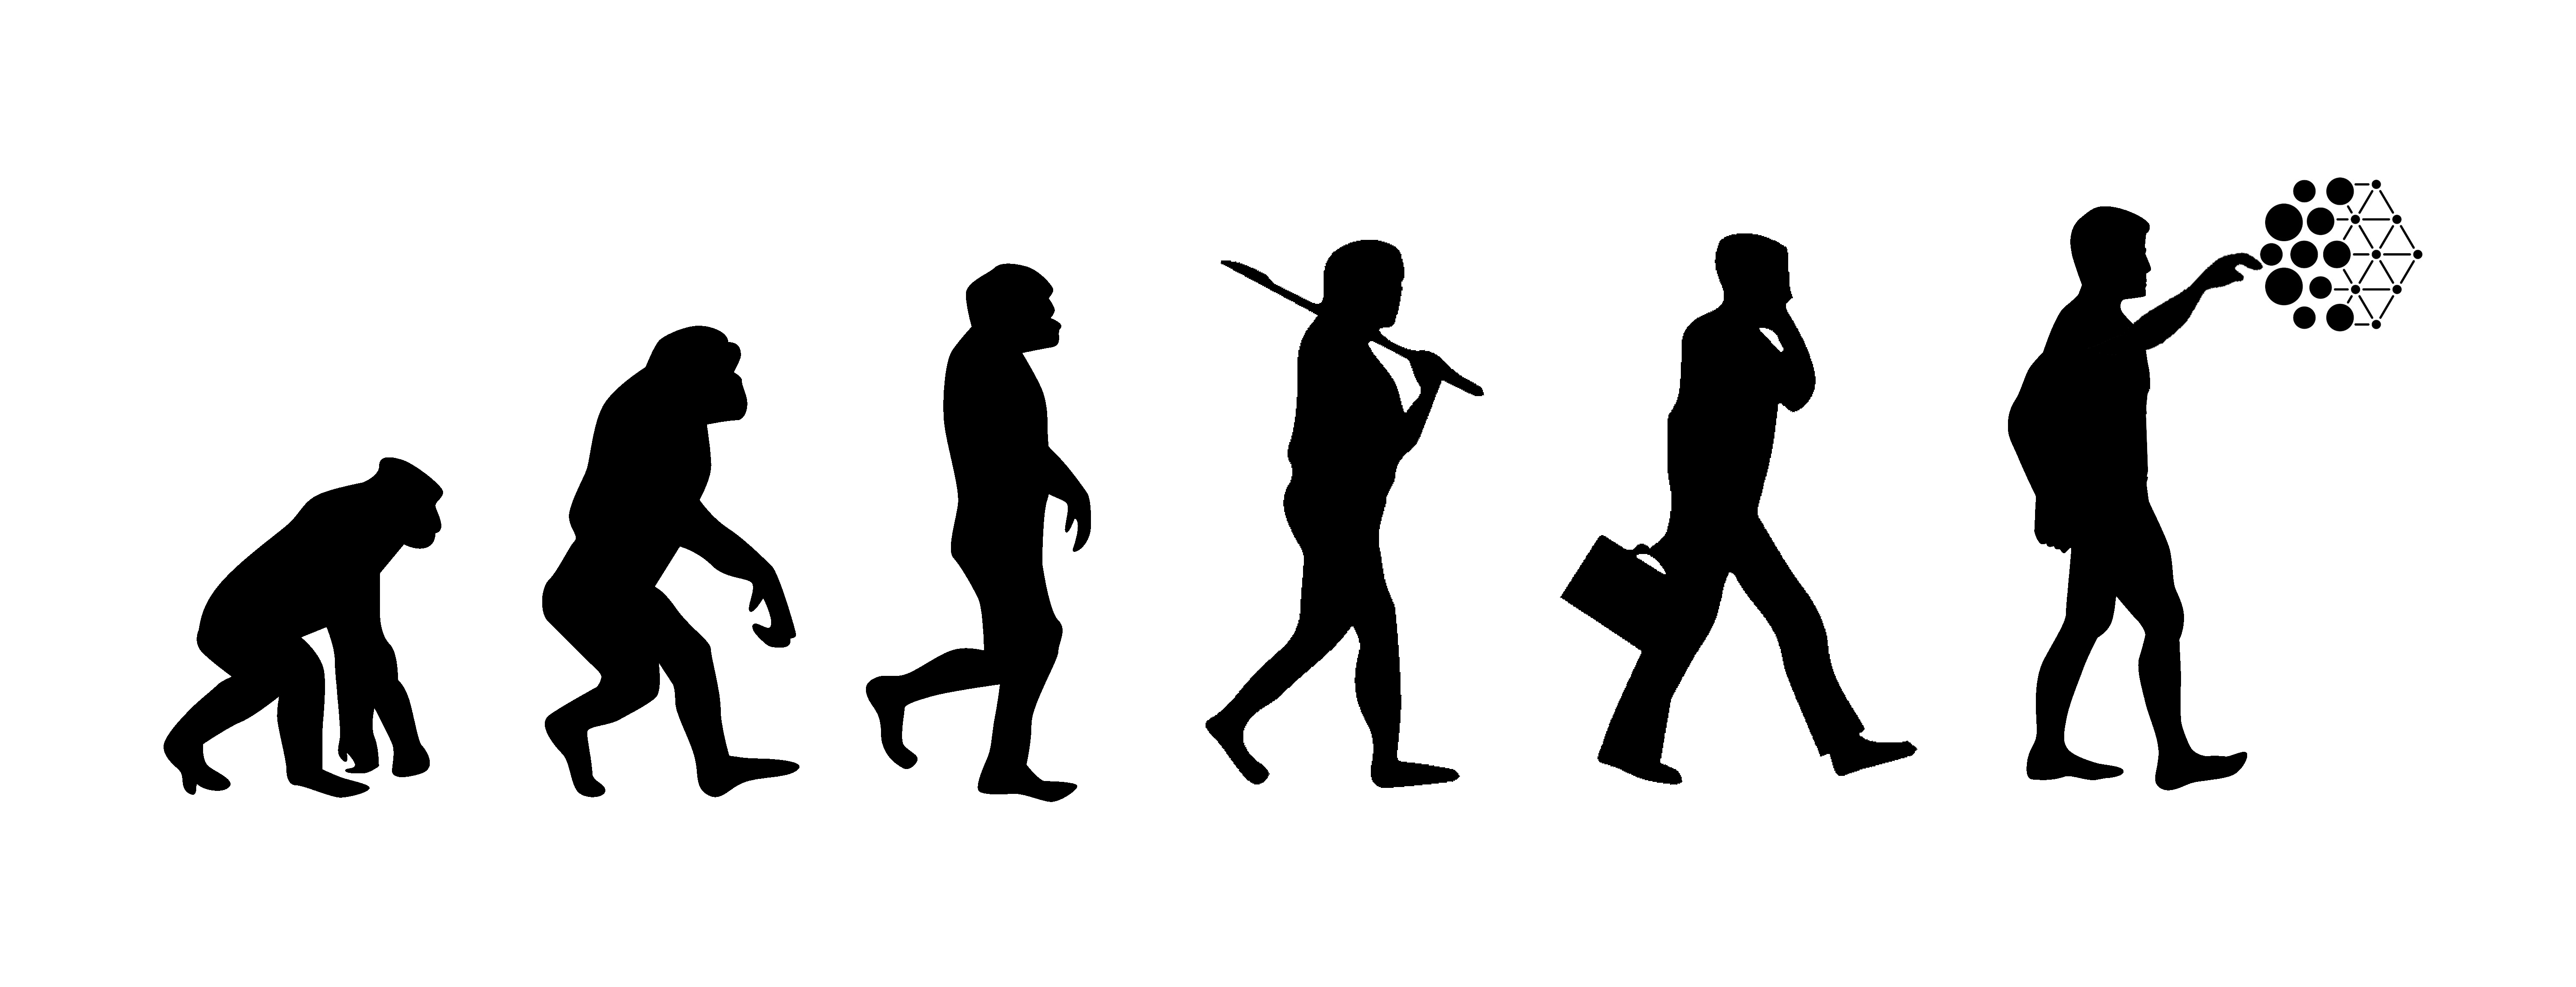
\includegraphics[width=0.90\textwidth]{../figures/evolution.png}
% 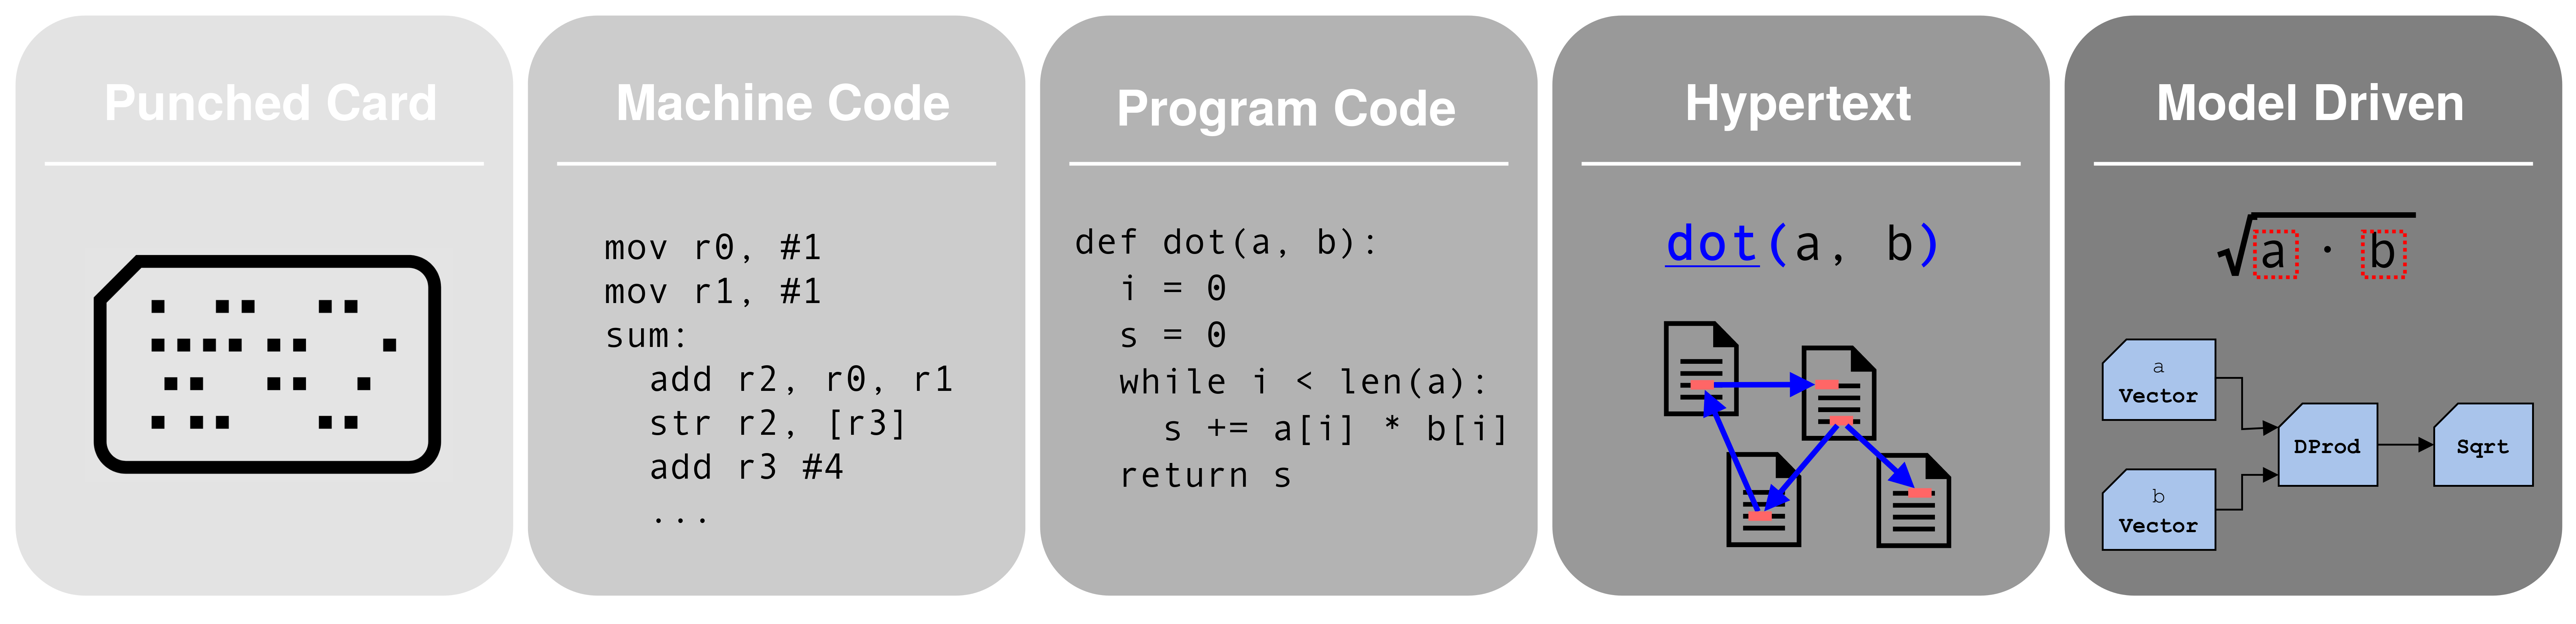
\includegraphics[width=0.90\textwidth]{../figures/progress_in_program.png}
% \caption{The evolution of code. A gauche, les langues qui obligent l'utilisateur à s'adapter à la machine. À droite, on trouve des représentations de plus en plus souples du code source.}
% \label{fig:evolution_of_programming}
%\end{figure}
%
%A l'aube de l'ère de l'information, notre espèce est à l'aube d'une nouvelle ère de l'adolescence. Les mêmes organes autrefois développés pour la planification des mouvements dans l'espace de configuration euclidienne sont utilisés d'une manière jamais imaginée par nos géniteurs. À cette époque, une seule vie et les esprits les plus brillants de notre génération suffisent à peine pour franchir les frontières de la connaissance humaine. Les ingénieurs doivent consacrer la première moitié de leur carrière intellectuelle à l'acquisition de connaissances. Les scientifiques peinent pendant des années à construire les infrastructures nécessaires à la réalisation d'expériences simples. Si nous devons faire pousser des branches plus hautes de notre arbre de la connaissance, envoyer des racines pivotantes dans des puits de compréhension plus profonds, les dotations de la nature ne peuvent pas nous mener bien loin. Si l'humanité veut atteindre son plein potentiel dans le temps qui lui est imparti, sa population croissante de travailleurs de la connaissance aura besoin d'un nouvel ensemble d'outils pour transcender la complexité croissante de l'innovation.
%
%Chaque étape du processus de création de connaissances est lourde d'une complexité fortuite découlant de l'acquisition et de la maîtrise d'une expertise spécifique à un domaine, de la découverte et du transfert de connaissances existantes, du processus de conception et de prototypage, de la validation et de la vérification de ces conceptions, et enfin de l'entretien et des aspects opérationnels de la mise en production des systèmes de connaissances. L'ensemble de cette entreprise requiert une quantité énorme de ressources humaines pour pouvoir chorégraphier efficacement. Dans l'industrie de l'information, ces personnes sont souvent appelées \textit{architectes}, \textit{ingénieurs}, \textit{développeurs}, \textit{programmeurs}, ou simplement \textit{codeurs}.\footnote{Confirmez n'importe lequel de ces camps et ils protesteront sûrement, mais les différences sont le plus souvent exagérées.} Selon certaines enquêtes~\citep{data2018global}, leur population devrait dépasser les 61 millions d'ici 2020, sans parler de la gestion et de l'administration de leurs activités sur le lieu de travail.
%
\citet{kernighan1976software} introduit d'abord le terme \textit{outils logiciels} dans le contexte des utilitaires en ligne de commande Unix, à peu près dans le même esprit que les outils proposés dans cette thèse. \citet{thrun2000towards, erez2015simulation} développer des outils basés sur le langage et la simulation pour le développement de la robotique dans le même esprit. D'une manière générale, nous considérons tout logiciel qui aide les utilisateurs engagés dans l'activité d'écriture de programmes informatiques, comme un \textit{outil de programmation}.

Dans cette thèse, nous faisons de petits pas vers la réduction de la complexité de la programmation des systèmes intelligents, grâce à des outils de programmation. Tout d'abord, nous présentons un plugin pour la construction d'applications robotiques (\autoref{ch:hatchery}). Ensuite, nous décrivons un langage spécifique à un domaine pour écrire des programmes différenciables (\autoref{ch:kotlingrad}). En utilisant notre DSL (\autoref{ch:difftest}) comme véhicule, nous développons un cadre contradictoire pour tester les programmes différentiables et démontrons empiriquement son efficacité par rapport à une méthode d'échantillonnage probabiliste. Nous discutons ensuite d'une solution basée sur un conteneur pour la reproduction de programmes robotiques, et plus largement de tout système logiciel embarqué ayant des capacités visuomotrices (\autoref{ch:ducker}). Enfin, dans \autoref{ch:conclusion} nous proposons quelques réflexions et prévisions pour l'avenir de la programmation des systèmes intelligents. Il reste encore beaucoup de travail à faire. Nous pensons que l'avenir est brillant et nous espérons que ceux qui se consacrent à sa construction s'inspireront des orientations proposées ici.

\clearpage

\section{Iconographie}

Tout au long de cette thèse, l'iconographie suivante est utilisée pour indiquer:
%
\begin{enumerate}
    \item[] \inlineimg{../figures/laptop_icon.png} & Commandes shell destinées à un ordinateur, ou sortie dérivée de celui-ci. \\
    \vspace{-0.2cm}\item[] \inlineimg{../figures/bnf_file.png} & Références GrammarKit \inline{.bnf}~\footnote{GrammarKit usage notes: \url{https://github.com/JetBrains/Grammar-Kit/blob/master/HOWTO.md}} \\
    \vspace{-0.2cm}\item[] \inlineimg{../figures/docker_icon.jpg} & Soit \inline{Dockerfile}~\footnote{Références Dockerfile: \url{https://docs.docker.com/engine/reference/builder/}} ou Docker Compose~\footnote{Compose la référence du fichier: \url{https://docs.docker.com/compose/compose-file/}} syntaxe. \\
    \vspace{-0.2cm}\item[] \inlineimg{../figures/raspi_icon.png} & Commandes shell qui doivent être exécutées sur un Raspberry Pi. \hspace{-.08em}\footnote{Raspberry Pi: \url{https://www.raspberrypi.org/}} \\
    \vspace{-0.2cm}\item[] \inlineimg{../figures/duckietown.png} & Commandes shell Duckietown (\inline{dts}).\hspace{-.08em}\footnote{Duckietown Shell: \url{https://github.com/duckietown/duckietown-shell-commands}} \\
    \vspace{-0.2cm}\item[] \inlineimg{../figures/launch_icon.png} & Fichiers roslaunch \inline{.launch}.\hspace{-.08em}\footnote{ROSLaunch XML: \url{https://wiki.ros.org/roslaunch/XML}} \\
    \vspace{-0.2cm}\item[] \inlineimg{../figures/python_icon.png} & Code source de Python.\hspace{-.08em}\footnote{Documentation Python: \url{https://www.python.org/doc/}} \\
    \vspace{-0.2cm}\item[] \inlineimg{../figures/kotlin_file.png} & Code source de Kotlin.\hspace{-.08em}\footnote{Documentation Kotlin: \url{https://kotlinlang.org/docs/reference/}}
\end{enumerate}

\chapter{Programming tools for robotics}\label{ch:hatchery}
\setlength{\epigraphwidth}{0.78\textwidth}
\epigraph{``The hope is that, in not too many years, human brains and computing machines will be coupled together very tightly, and that the resulting partnership will think as no human brain has ever thought and process data in a way not approached by the information-handling machines we know today.''}{\begin{flushright}--Joseph \citet{licklider1960man}, \href{https://groups.csail.mit.edu/medg/people/psz/Licklider.html}{\textit{Man-Computer Symbiosis}}\end{flushright}}

In this chapter we will discuss the design and implementation of an integrated development environment (IDE) for building intelligent robotic software. Modern robots are increasingly driven by systems which learn and improve over time. Most researchers would agree that modern robotic systems have not yet achieved biologically competitive sensorimotor capabilities and most intelligent systems are not physically embodied. However, it is our view that any closed-loop control system that is not explicitly programmed to perform a specific task, but which learns it from experience is an \textit{intelligent system}. Furthermore, any closed-loop system with physical motors is a \textit{robotic system}. While research has demonstrated successful applications in both areas separately, it is widely believed the integration of intelligent systems and robotics will be tremendously fruitful when fully realized.

Hatchery is a tool designed to assist programmers writing robotics applications using the ROS middleware. At the time of its release, \href{https://github.com/duckietown/hatchery}{Hatchery} was the first ROS plugin for the \href{https://www.jetbrains.org/intellij/sdk/docs}{IntelliJ Platform} \footnote{An IDE platform for C/C++, Python and Android development, among other languages.}, and today, is the most widely used with over 10,000 unique downloads. While the idea is simple, its prior absence and subsequent adoption suggest there is unmet demand for such tools in the development of intelligent software systems, particularly in domain-specific applications like robotics.
%

\begin{figure}
    \centering
    \begin{tikzpicture}
        \begin{axis}[
            ybar, ymin=0,
            ylabel=Downloads,
            date coordinates in=x,
            xmin=2017-12-01,
            xmax=2019-06-01,
            xtick=data,
            xticklabel style={
                rotate=70,
                anchor=near xticklabel,
            },
            xticklabel=\year-\month,
            nodes near coords,
            nodes near coords align={vertical},
            height=0.25\textwidth,
            width=0.95\textwidth,
            enlarge x limits=0.03,
            axis x line*=bottom,
            axis y line*=left,
            tick pos=left,
            compat=newest,
        ]
            \addplot table[col sep=comma, x=Category,y=Downloads]{../data/hatchery_downloads.csv};
        \end{axis}
        \node[above,font=\large\bfseries] at (current bounding box.north) {Unique downloads of Hatchery};
    \end{tikzpicture}
    \caption{Unique downloads of Hatchery between the time of its release and June 2019. \url{https://plugins.jetbrains.com/plugin/10290-hatchery}.}
    \label{fig:hatchery_downloads}
\end{figure}
%
\section{Introduction to the Robot Operating System}

The \href{https://www.ros.org/}{Robot Operating System} (ROS)~\citep{quigley2009ros} is a popular middleware for robotics applications. At its core, ROS provides software infrastructure for distributed messaging, but also includes a set of community-developed libraries and graphical tools for building robotics applications. ROS is not an operating system (OS) in the traditional sense, but it does support similar functionality such as shared memory and inter-process communication. Unlike pure message-oriented systems such as DDS~\citep{pardo2003omg} and \href{https://zeromq.org/}{ZMQ}~\citep{hintjens2013zeromq}, in addition to the communication infrastructure, ROS provides specific APIs for building decentralized robotic systems, particularly those which are capable of mobility. This includes standard libraries for serializing and deserializing geometric data, coordinate frames, maps, sensor messages, and imagery.

The ROS middleware provides several language front-ends for polyglot programming. According to one community census taken in 2018, 55\% of all ROS applications on GitHub are written in C/C++, followed by Python with a 25\%~\citep{Areserio54:online} developer share. Source code for a typical ROS application contains a mixture of C/C++ and Python code, corresponding to the respective language preferences in the robotics and machine learning communities. Hatchery is compatible with most common ROS client libraries, including \href{https://wiki.ros.org/rosjava}{rosjava} for Java, \href{https://wiki.ros.org/rospy}{rospy} for Python, \href{https://wiki.ros.org/rospy}{roscpp} for C/C++, and other language front ends.

\begin{figure}
    \centering
    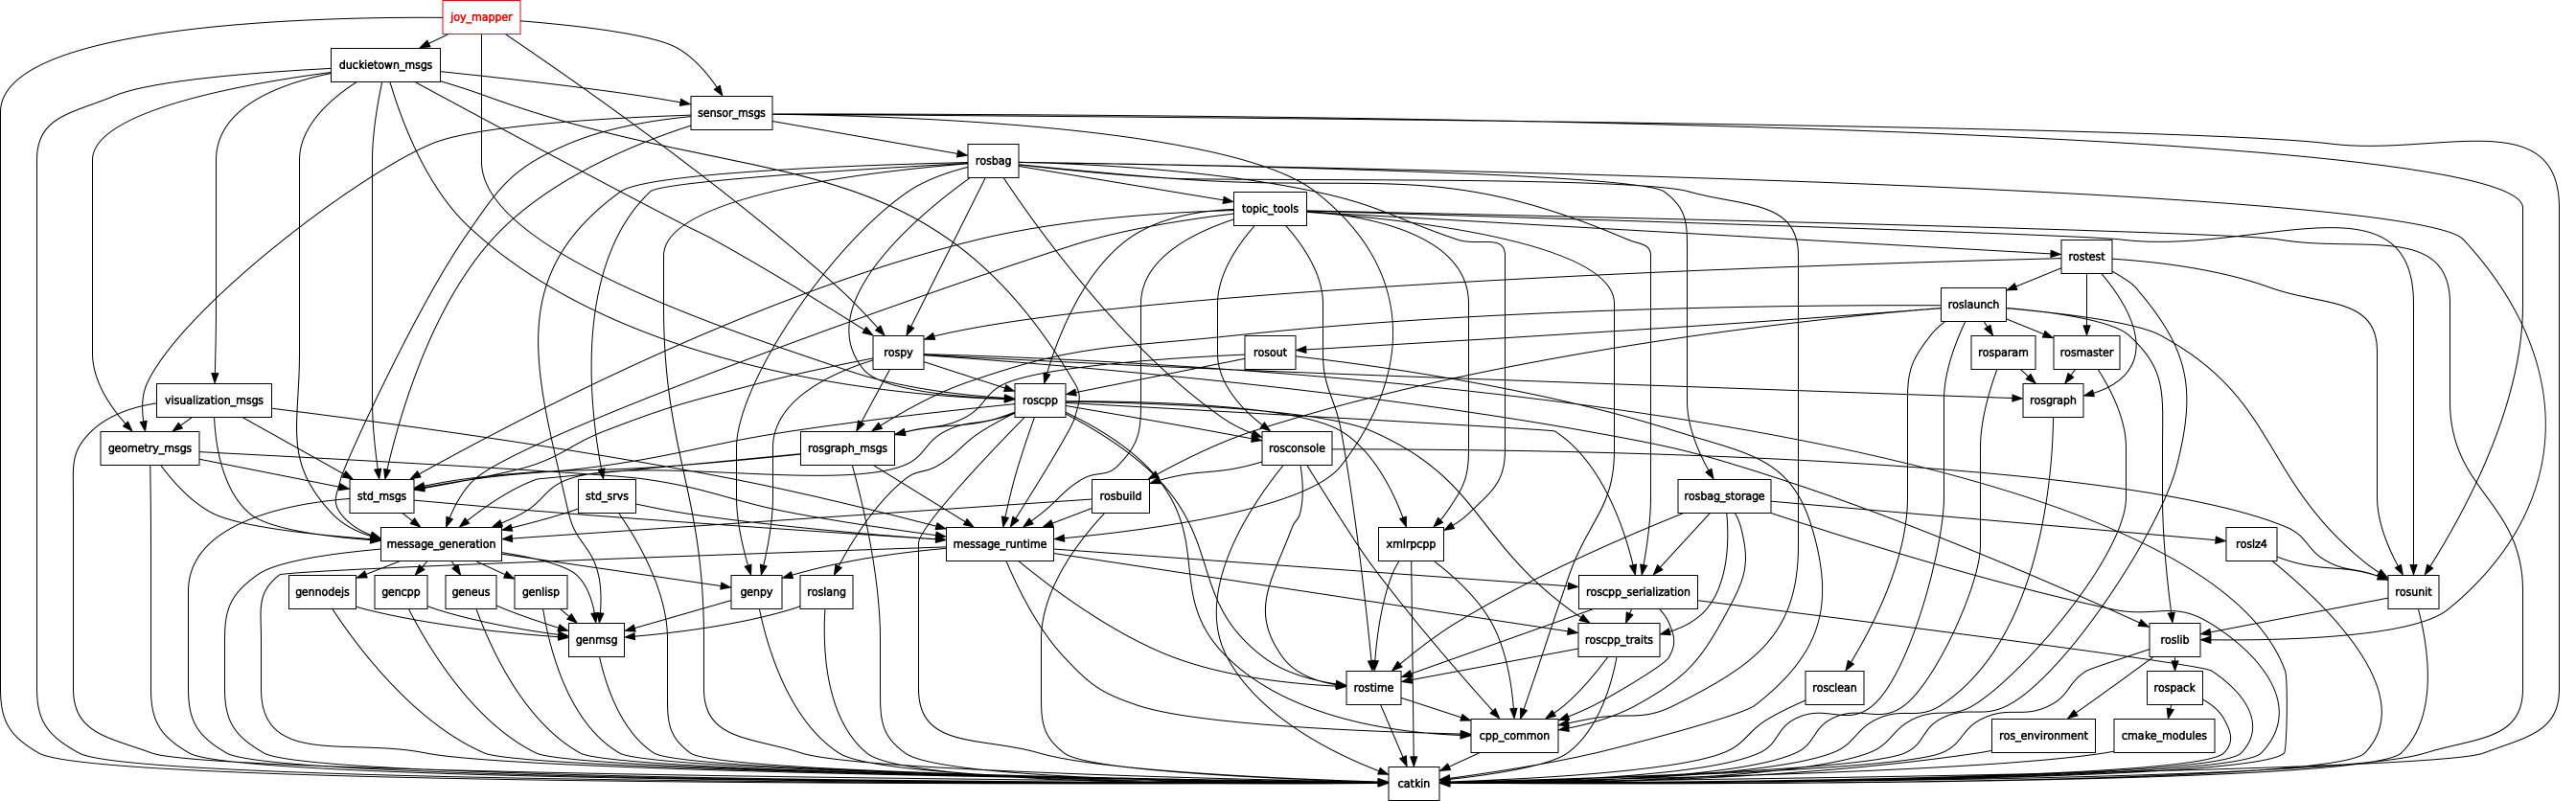
\includegraphics[width=\textwidth]{../figures/rqt_dep_graph.png}
    \caption{A typical ROS application contains a large graph of dependencies.}
\end{figure}

A typical ROS project has several components, including the source code, configuration files, build infrastructure, compiled artifacts and the deployment environment. To build a simple ROS application, several steps are necessary. First, one must install the ROS system, which is only officially supported on Debian-based Linux distributions.\hspace{-.08em}\footnote{Detailed installation instructions may be found here: \url{https://wiki.ros.org/ROS/Installation}}
%
Assuming ROS has been installed to the default location, it can be sourced like so:
%
\begin{pclisting}
    ~$ source /opt/ros/<ROS DISTRO>/setup.[ba]sh
\end{pclisting}
%
A minimal ROS application contains at least one \textit{publisher} and \textit{subscriber}, which pass messages over a shared communication channel. The publisher might be defined as follows:
%
\begin{pythonlisting}[title=./catkin\_ws/src/pubsub/publisher.py]
import rospy
from std_msgs.msg import String

pub = rospy.Publisher("(*\hl{channel}*)", String, queue_size=10)
rospy.init_node("publisher", anonymous=True)
rate = rospy.Rate(10)
while not rospy.is_shutdown():
pub.publish("Some message")
rate.sleep()
\end{pythonlisting}
%
As the publisher writes messages to \hl{\ttfamily\small channel}, another node which is subscribed to the same channel will receive a callback when new messages arrive and can read them off the channel:
%
\begin{pythonlisting}[title=./catkin\_ws/src/pubsub/subscriber.py]
def callback(data):
rospy.loginfo(rospy.get_caller_id() + "received data %s", data.data)

rospy.init_node("subscriber", anonymous=True)
rospy.Subscriber("(*\hl{channel}*)", String, callback)
rospy.spin()
\end{pythonlisting}
%
All ROS packages have launch file, which contain a manifest of available nodes:
%
\begin{launchlisting}[title=./catkin\_ws/src/pubsub/pubsub.launch]
<launch>
<node name="publisher" pkg="pubsub" type="publisher.py" output="screen"/>
<node name="subscriber" pkg="pubsub" type="subscriber.py" output="screen"/>
</launch>
\end{launchlisting}
%
To build and run the application, the following series of commands are required:
%
\begin{pclisting}
    ~$ cd catkin_ws && catkin_make
\end{pclisting}
%
\begin{pclisting}
~$ roslaunch pubsub pubsub.launch
\end{pclisting}
%
Rather than interacting with the command line, it would be convenient to have a graphical tool to perform all of these tasks automatically. Additionally, it would be helpful to detect if there were a typographical error or navigable reference in the launch file:
%
\begin{launchlisting}[title=./catkin\_ws/src/pubsub/pubsub.launch]
<launch>
<node name="publisher" pkg="pubsub" type="(*\color{red}\textbf{pubsher.py}*)" output="screen"/>
<node name="subscriber" pkg="pubsub" type="(*\color{blue}\underline{subscriber.py}*)" output="screen"/>
</launch>
\end{launchlisting}
%
Notice how the typographical error is printed in red and the valid file reference is underlined in blue, indicating it can be selected to open the file shown above. Broadly, these are the kinds of features IDEs provide and are examples of specific functionality in Hatchery.

\section{Installation}\label{subsec:installation}

\noindent To simply run the tool, users should have the following software dependencies:
%
\begin{enumerate}
\item MacOS or Debian-based Linux distribution
\item Robot Operating System (Electric Emys or later)
\item Java SE (JRE 8+) or CLion/PyCharm 2019.1+
\end{enumerate}
%
\noindent ROS users can use the following command to open an existing ROS project:
%
\begin{pclisting}
~$ git clone https://github.com/duckietown/hatchery && cd hatchery && \
   ./gradlew runIde [-Project="<ABSOLUTE_PATH_TO_ROS_PROJECT>"]
\end{pclisting}
%
\noindent Duckietown users can simply use \inline{dts}, the Duckietown Shell:
%
\begin{dtslisting}
dt> hatchery
\end{dtslisting}
%
\noindent Hatchery can also be installed directly from inside the CLion or PyCharm IDEs, via the following menu options: \menu{File > Settings > Plugins > Marketplace > {\faSearch ``Hatchery''}}

\section{Plugin development}

To build an IDE, some tools are helpful. First, is an IDE, and its source code. Assume that IDE\textsubscript{0} exists. In order to build a new IDE, IDE\textsubscript{1}, we can load the source code from IDE\textsubscript{0} into IDE\textsubscript{0} and use IDE\textsubscript{0}, to modify, compile and re-run the code, which becomes IDE\textsubscript{1}, in which the process is repeated. However, this approach has some disadvantages. First, most IDEs are already quite cumbersome to compile and run. As most auxiliary features are small by comparison, modern IDEs have adopted a modular design, which allows them to load specific packages (i.e.\ \textit{plugins}) as needed. So most developers can skip the first step, and load their plugin inside IDE\textsubscript{0} directly. It is still convenient to have the platform source code for reference purposes, but in most cases this code is read-only.

Hatchery uses the \href{https://www.jetbrains.org/intellij/sdk/docs/}{IntelliJ Platform}, an IDE platform which supports most common programming languages. By targeting a platform with support for polyglot programming, we are able to focus on language-agnostic features in the ROS ecosystem, such as parsing and editing ROS-specific configuration files, build and run configuration and other common development tasks.

\subsection{Refactoring}\label{subsec:refactoring}

Refactoring is an essential feature in any IDE, and the essence of refactoring is renaming. Consider what must occur when a user wishes to rename a token in her program, such as the parameter named \inline{data} on line \#1 below:
%
\begin{pythonlisting}
def callback(data):
rospy.loginfo(rospy.get_caller_id() + "received data: %s", data.data)
\end{pythonlisting}
%
If she were using the \inline{vim} text editor, one solution would be to replace all textual occurrences of the string \inline{data} within the file using \inline{:\%s/data/msg/g}, producing the following result:
%
\begin{pythonlisting}
def callback((*\hl{msg}*)):
rospy.loginfo(rospy.get_caller_id() + "received (*\hl{msg}*): %s", (*\hl{msg}*).(*\hl{msg}*))
\end{pythonlisting}
%
There were four occurrences of the string \inline{data}, only two of which were correctly renamed. Instead, only those strings which refer to the function parameter should be renamed:
%
\newcommand{\cfbox}[2]{\colorlet{currentcolor}{.}{\color{#1}\fbox{\color{currentcolor}#2}}}

\begin{pythonlisting}
def callback((*\cfbox{red}{data}*)):
rospy.loginfo(rospy.get_caller_id() + "received data: %s", (*\cfbox{red}{data}*).data)
\end{pythonlisting}
%
Generally, we would like the ability to rename identifiers across files and languages. To do so, we need a richer understanding of code that transcends text -- we need a parser.

\subsection{Parsing}\label{subsec:the-parser}

One of the most important and unappreciated components of an IDE is the parser. Unlike compilers, most IDEs do not use recursive descent or shift-reduce parsing as treated in most compiler textbooks~\citep{appel2003modern}, as these algorithms are not well-suited for real-time editing of source code. Edits are typically short, localized changes inside a large file, and are frequently invalid or incomplete between keystrokes. As most IDEs are expected to recover from local errors and provide responsive feedback while editing source code, re-parsing the entire program between minor edits would be expensive and unnecessary. In order to analyze source code undergoing simultaneous modification and provide interactive feedback, special consideration must be taken to ensure robust and responsive parsing.

Various techniques have been developed to improve the responsiveness of modern parsers. Incremental parsing techniques like those first proposed in \citet{ghezzi1979incremental} and further developed by \citet{wagner1997practical,wagner1997incremental} seek to incorporate caching and differential parsing to accelerate the analysis of programs under simultaneous modification. Fuzzy parsing techniques like those described in ~\citet{koppler1997systematic} aim to increase the flexibility and robustness of parsing in the presence of local errors. Both of these techniques have played a role in the development of language-aware programming tools, which must be able to provide rapid and specific feedback whilst the user is typing.

The procedural instructions for modern parsers are seldom written by hand unless the language being parsed is very simple or raw performance is desired. Even parsers designed for IDEs, where incremental parsing and error-tolerance is so important, metacompilation toolkits such as ANTLR~\citep{parr1995antlr}, or Xtext~\citep{eysholdt2010xtext} cover a surprising number of common use-cases. Hatchery uses \href{https://github.com/JetBrains/grammar-kit}{Grammar-Kit}, a toolkit designed to assist users developing custom language plugins for the \href{https://www.jetbrains.org/intellij/sdk/docs}{IntelliJ Platform}. It uses a DFA-based lexer generator, JFlex~\citep{klein2001jflex}, and a custom parser-generator loosely based on the parsing expression grammar (PEG)~\citep{ford2004parsing}, a descendant of the Backus-Naur Form (BNF) grammar specification. This specification is consumed by the GrammarKit parser generator and translated to Java source code, producing a parser which reads source code written in the specified language and constructs a program structure interface (PSI), the IntelliJ Platform's internal data structure for representing abstract syntax trees (ASTs). Here is an excerpt of a PEG BNF grammar for parsing ROS \href{https://wiki.ros.org/msg}{\inline{.msg}} files:
%
\begin{bnflisting}
rosInterfaceFile ::= ( property | COMMENT )*
property ::= ( TYPE FIELD SEPARATOR CONSTANT ) | ( TYPE FIELD ) {
pin=3 // Identifies an unambiguous delimiter or fallback point
recoverWhile="recover_property" // Error recovery predicate
mixin="edu.umontreal.hatchery.psi.impl.RosMsgNamedElementImpl"
implements="edu.umontreal.hatchery.psi.RosMsgNamedElement"
methods=[getType getKey getValue getName setName getNameIdentifier]
}
private recover_property ::= ! ( TYPE | FIELD | SEPARATOR | COMMENT )
\end{bnflisting}
%
\begin{figure}
\centering
% To regenerate: https://homepage.ruhr-uni-bochum.de/jan.holthuis/posts/using-the-latex-rail-package#manual-compilation-and-latexmk-support
\begin{rail}
( [2] TYPE FIELD ( () | SEPARATOR CONSTANT) ) | ( [1] COMMENT )
\end{rail}
\caption{Railroad diagram for the grammar shown above (reads from left to right).}
\label{fig:railroad}
\end{figure}
%
The lexical rules for the tokens, \inline{TYPE}, \inline{FIELD}, \inline{CONSTANT} et al. are defined in a separate \inline{.flex} file, the \href{https://www.jflex.de/manual.html#Grammar}{JFlex grammar}. Below is an excerpt from the accompanying \inline{.flex} lexer:
%
\begin{flexlisting}
TYPE_CHARACTER=[^:=#\ \r\n\t\f\\]
FIELD_CHARACTER=[^:=#\ \r\n\t\f\\]
SEPARATOR_CHARACTER=[:=]
CONSTANT_CHARACTER=[^\r\n\f#]
COMMENT_CHARACTER=#[^\r\n\f]*
\end{flexlisting}

Grammar-Kit consumes these files and generates Java source code for parsing ROS \href{https://wiki.ros.org/msg}{\inline{.msg}} files. Generated sources can be manually refined to provide support for more advanced functionality such as more flexible error-recovery. For regular languages like the interface description languages (IDL) found in ROS \href{https://wiki.ros.org/msg}{\inline{.msg}} and \href{https://wiki.ros.org/srv}{\inline{.srv}} files, the default generated parser and lexer are usually sufficient. Hatchery is also capable of parsing \href{https://wiki.ros.org/urdf}{URDF}, \href{https://wiki.ros.org/Manifest}{package manifest} and \href{https://wiki.ros.org/roslaunch/XML}{roslaunch} XML.

\subsection{Running and debugging}

The process of compiling and running ROS applications often requires several steps, ex.:
%
\begin{pclisting}
~$ . /opt/ros/<DISTRO>/setup.[ba]sh &&
cd <PROJECT>/catkin_ws &&
catkin_make &&
. devel/setup.sh &&
[export ROS_MASTER_URI=<URI> &&]
roslaunch [OPTIONS] src/.../<LAUNCH FILE> [ARGUMENTS]"
\end{pclisting}
%
Hatchery provides assistance for configuring, building and running ROS applications inside a custom graphical user interface (GUI). This GUI effectively serves as a wrapper for the ROS command line interface (CLI). Visual elements like configuration options and command line flags are written to an internal model called the ``Run Configuration'' (\autoref{fig:ros_run_config}). When a run configuration is manually triggered, Hatchery's internal model is serialized to a \inline{String}, representing the command to be executed. This \inline{String} is then sent to a terminal emulator, which invokes the command and displays the corresponding output.

\begin{figure}
\centering
\frame{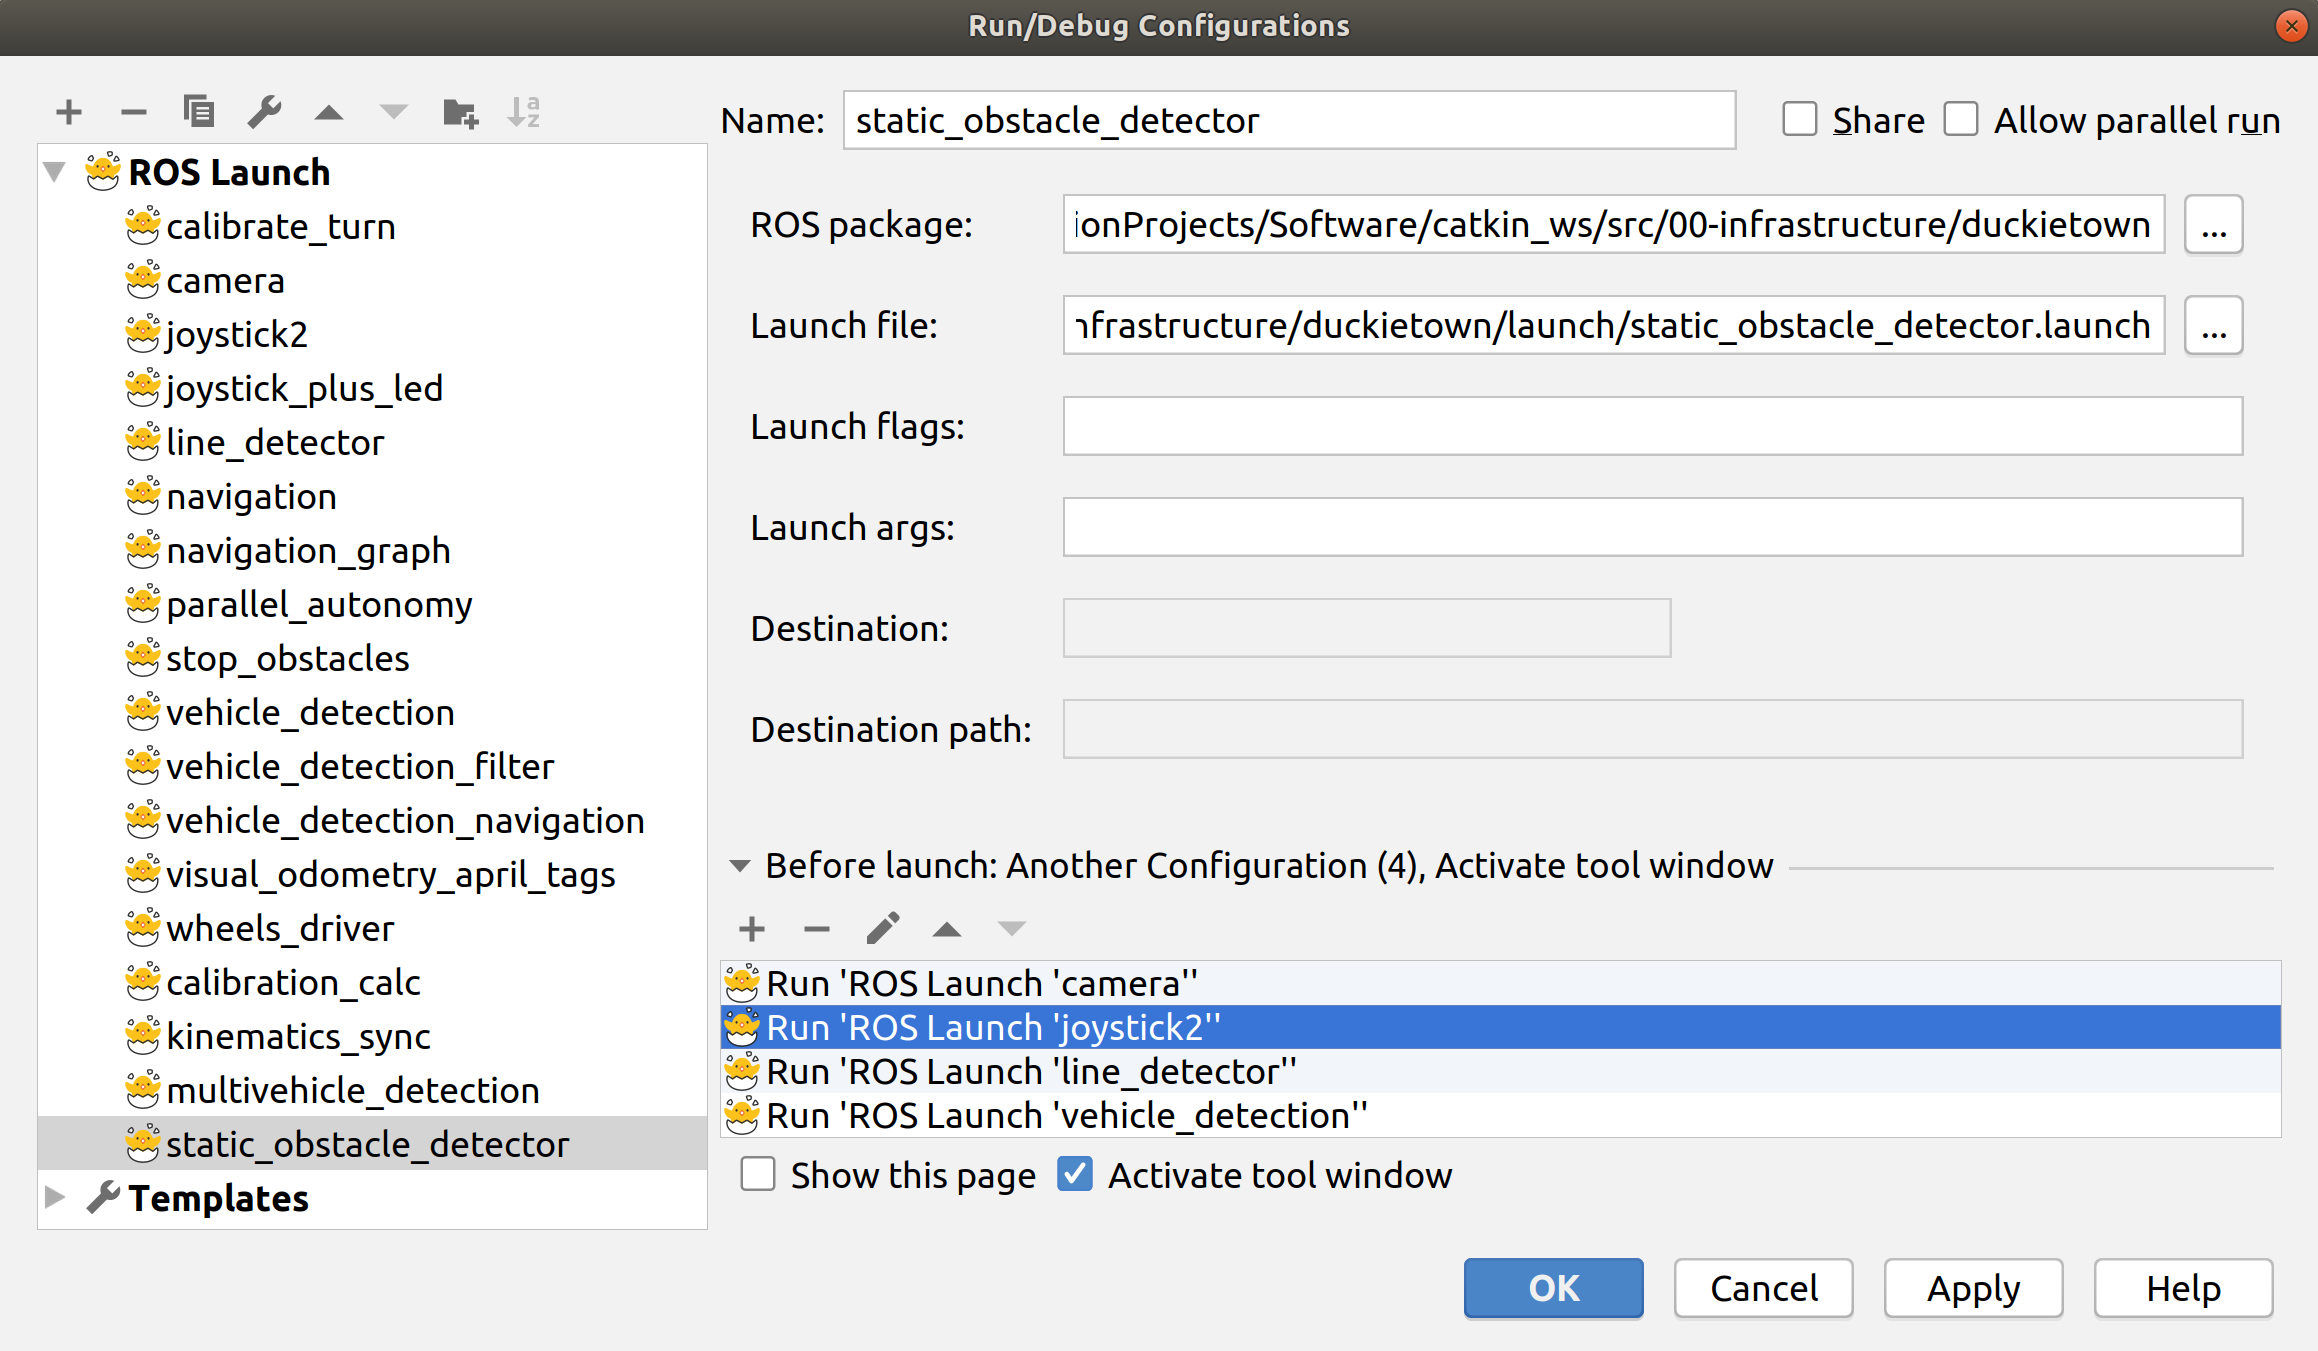
\includegraphics[width=0.90\textwidth]{../figures/ros_run_config.png}}
\caption{ROS Run Configuration. Accessible via: \menu{Run > Edit Configurations > + > ROS Launch}}
\label{fig:ros_run_config}
\end{figure}

\subsection{User interface}

An often overlooked, but important aspect of development tools is the graphical user interface, as the primary interface for editing source code. In the early days of modern computing, the only way of getting information in or out of a computer involved punching holes in paper. Later, computers were equipped with technology to emit the same binary pattern as pixels, which could be used to display a small alphabet called ASCII. With higher density and frequency displays, computers could render more sophisticated shapes and animations. These improvements are the direct result of graphical innovation, but can also be seen as progress in program representation, where the symbolic medium was itself just a notational convention which developers and machines used to communicate.

\begin{figure}
\centering
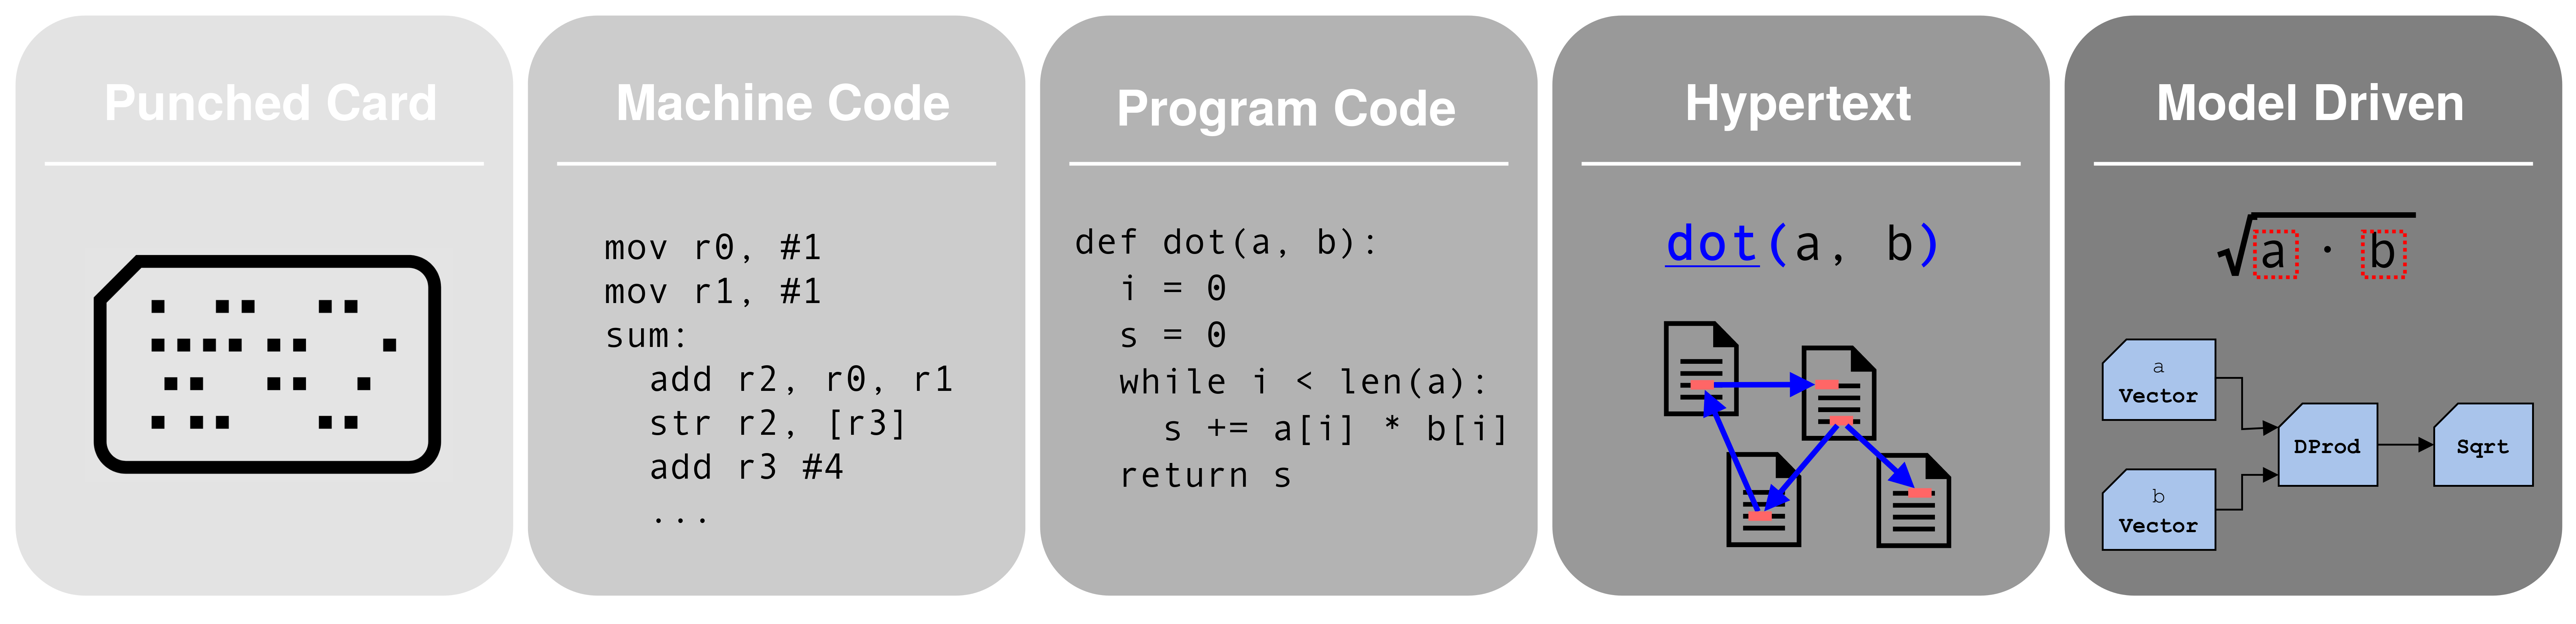
\includegraphics[width=0.90\textwidth]{../figures/progress_in_program.png}
\caption{The evolution of code. On the left are languages that force the user to adapt to the machine. To the right are increasingly flexible representations of source code.}
\label{fig:evolution_of_programming}
\end{figure}

ASCII is still the dominant medium for modern programming, although machines still use various forms of low-level assembly code for execution. A great deal of software infrastructure is dedicated to translating between such representations via programming languages and compilers. While many software frameworks provide a minimal command line interface (CLI) and some even provide sophisticated programming environments, these tools are fairly restrictive. In the same way that early computer scientists probably did not invent new algorithms by imagining patterns of holes in paper, ASCII is also an indirect medium for expressing ideas, albeit one slightly less contrived. As hardware and software technology progressed, programming languages moved ``up the stack'', allowing their users to express ideas in a notation which was more familiar and easy to reason about its execution.

\begin{figure}
\centering
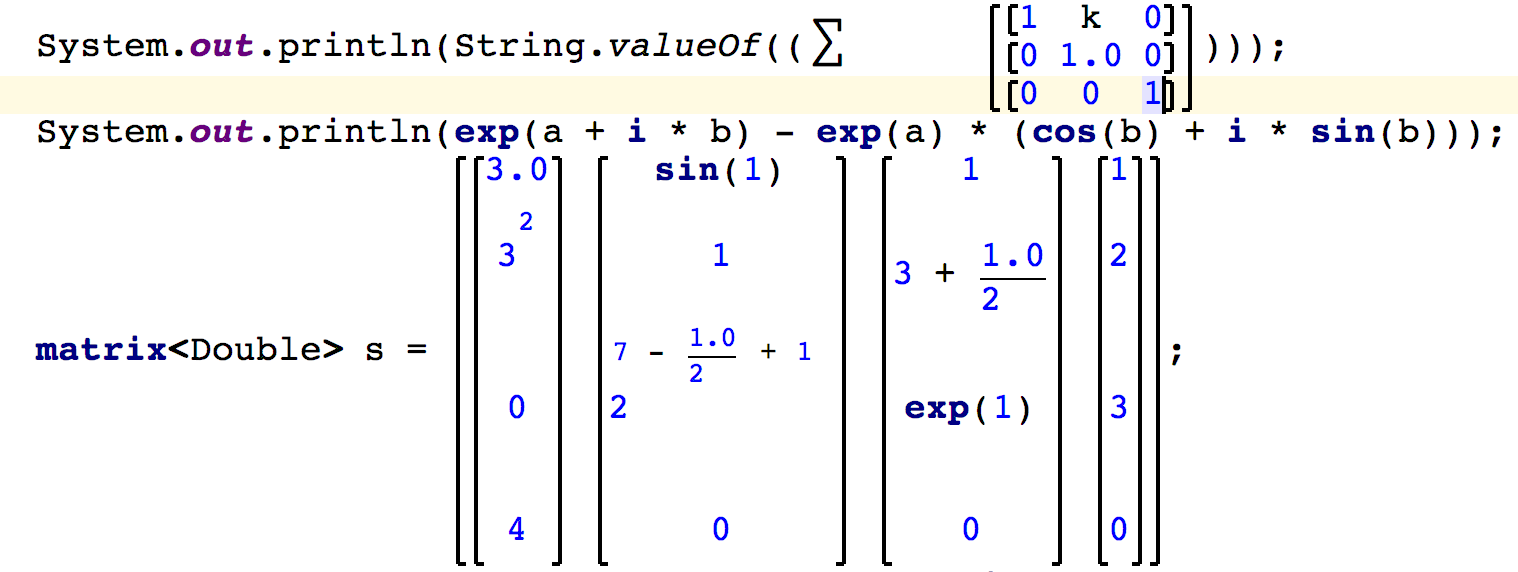
\includegraphics[width=0.90\textwidth]{../figures/mps_screenshot.png}
\caption{Projectional editors such as \href{https://www.jetbrains.com/mps/}{MPS}~\citep{voelter2010language, pech2013jetbrains} (shown above) are able to render source code in visually creative ways. This might resemble freehand notation or some other visually appealing format.}
\label{fig:mps_screenshot}
\end{figure}

With the development of modern languages came programming tools capable of representing code as a mixture of hypertext and graphical user interfaces. Such tools provide a richer representation for code than plaintext and help to capture programs' graph-based structure, but still use ASCII with sparse visual cues to render code. Some tools support larger character sets and font-based typographic ligatures, although the visual representation of source code remains mostly linear and textual.

More experimental UIs, as proposed in the language oriented programming~\citep{dmitriev2004language} and model-driven engineering~\citep{famelis2015mummint} literature, suggest the possibility of more visually flexible layouts. This uncoupling between the composition and representation of text raises many intriguing questions. With the proliferation of new abstractions and programming shorthands, what is the appropriate level of notation required for a given programming task? And who is the intended audience? These are important questions to consider when designing a new programming tool.

The Hatchery plugin provides a lightweight GUI overlaying the program's source code. This interface (\autoref{fig:hatchery_gui}) primarily consists of simple visual cues such as text highlighting, navigation assistance and other menus and configuration panels for performing various programming tasks. The host IDE offers a visual language consisting of iconography and repetitive visual motifs, which serve as cognitive landmarks to guide the developer's procedural memory. The IntelliJ Platform offers a palette of common design elements, which users who are familiar with the IDE can recognize at a glance. Plugins can use these same patterns to access procedural memories implanted in the userbase, facilitating transfer learning. To do this properly requires familiarity with the design language and careful integration with the target framework (i.e. ROS).

Hatchery provides a settings menu for configuring and managing ROS installations which can automatically detect local ROS distributions and also allows users to manually configure the \href{https://wiki.ros.org/ROS/Tutorials/InstallingandConfiguringROSEnvironment}{ROS environment}, as shown in ~\autoref{fig:ros_settings}.
%
\begin{figure}[b]
\centering
\frame{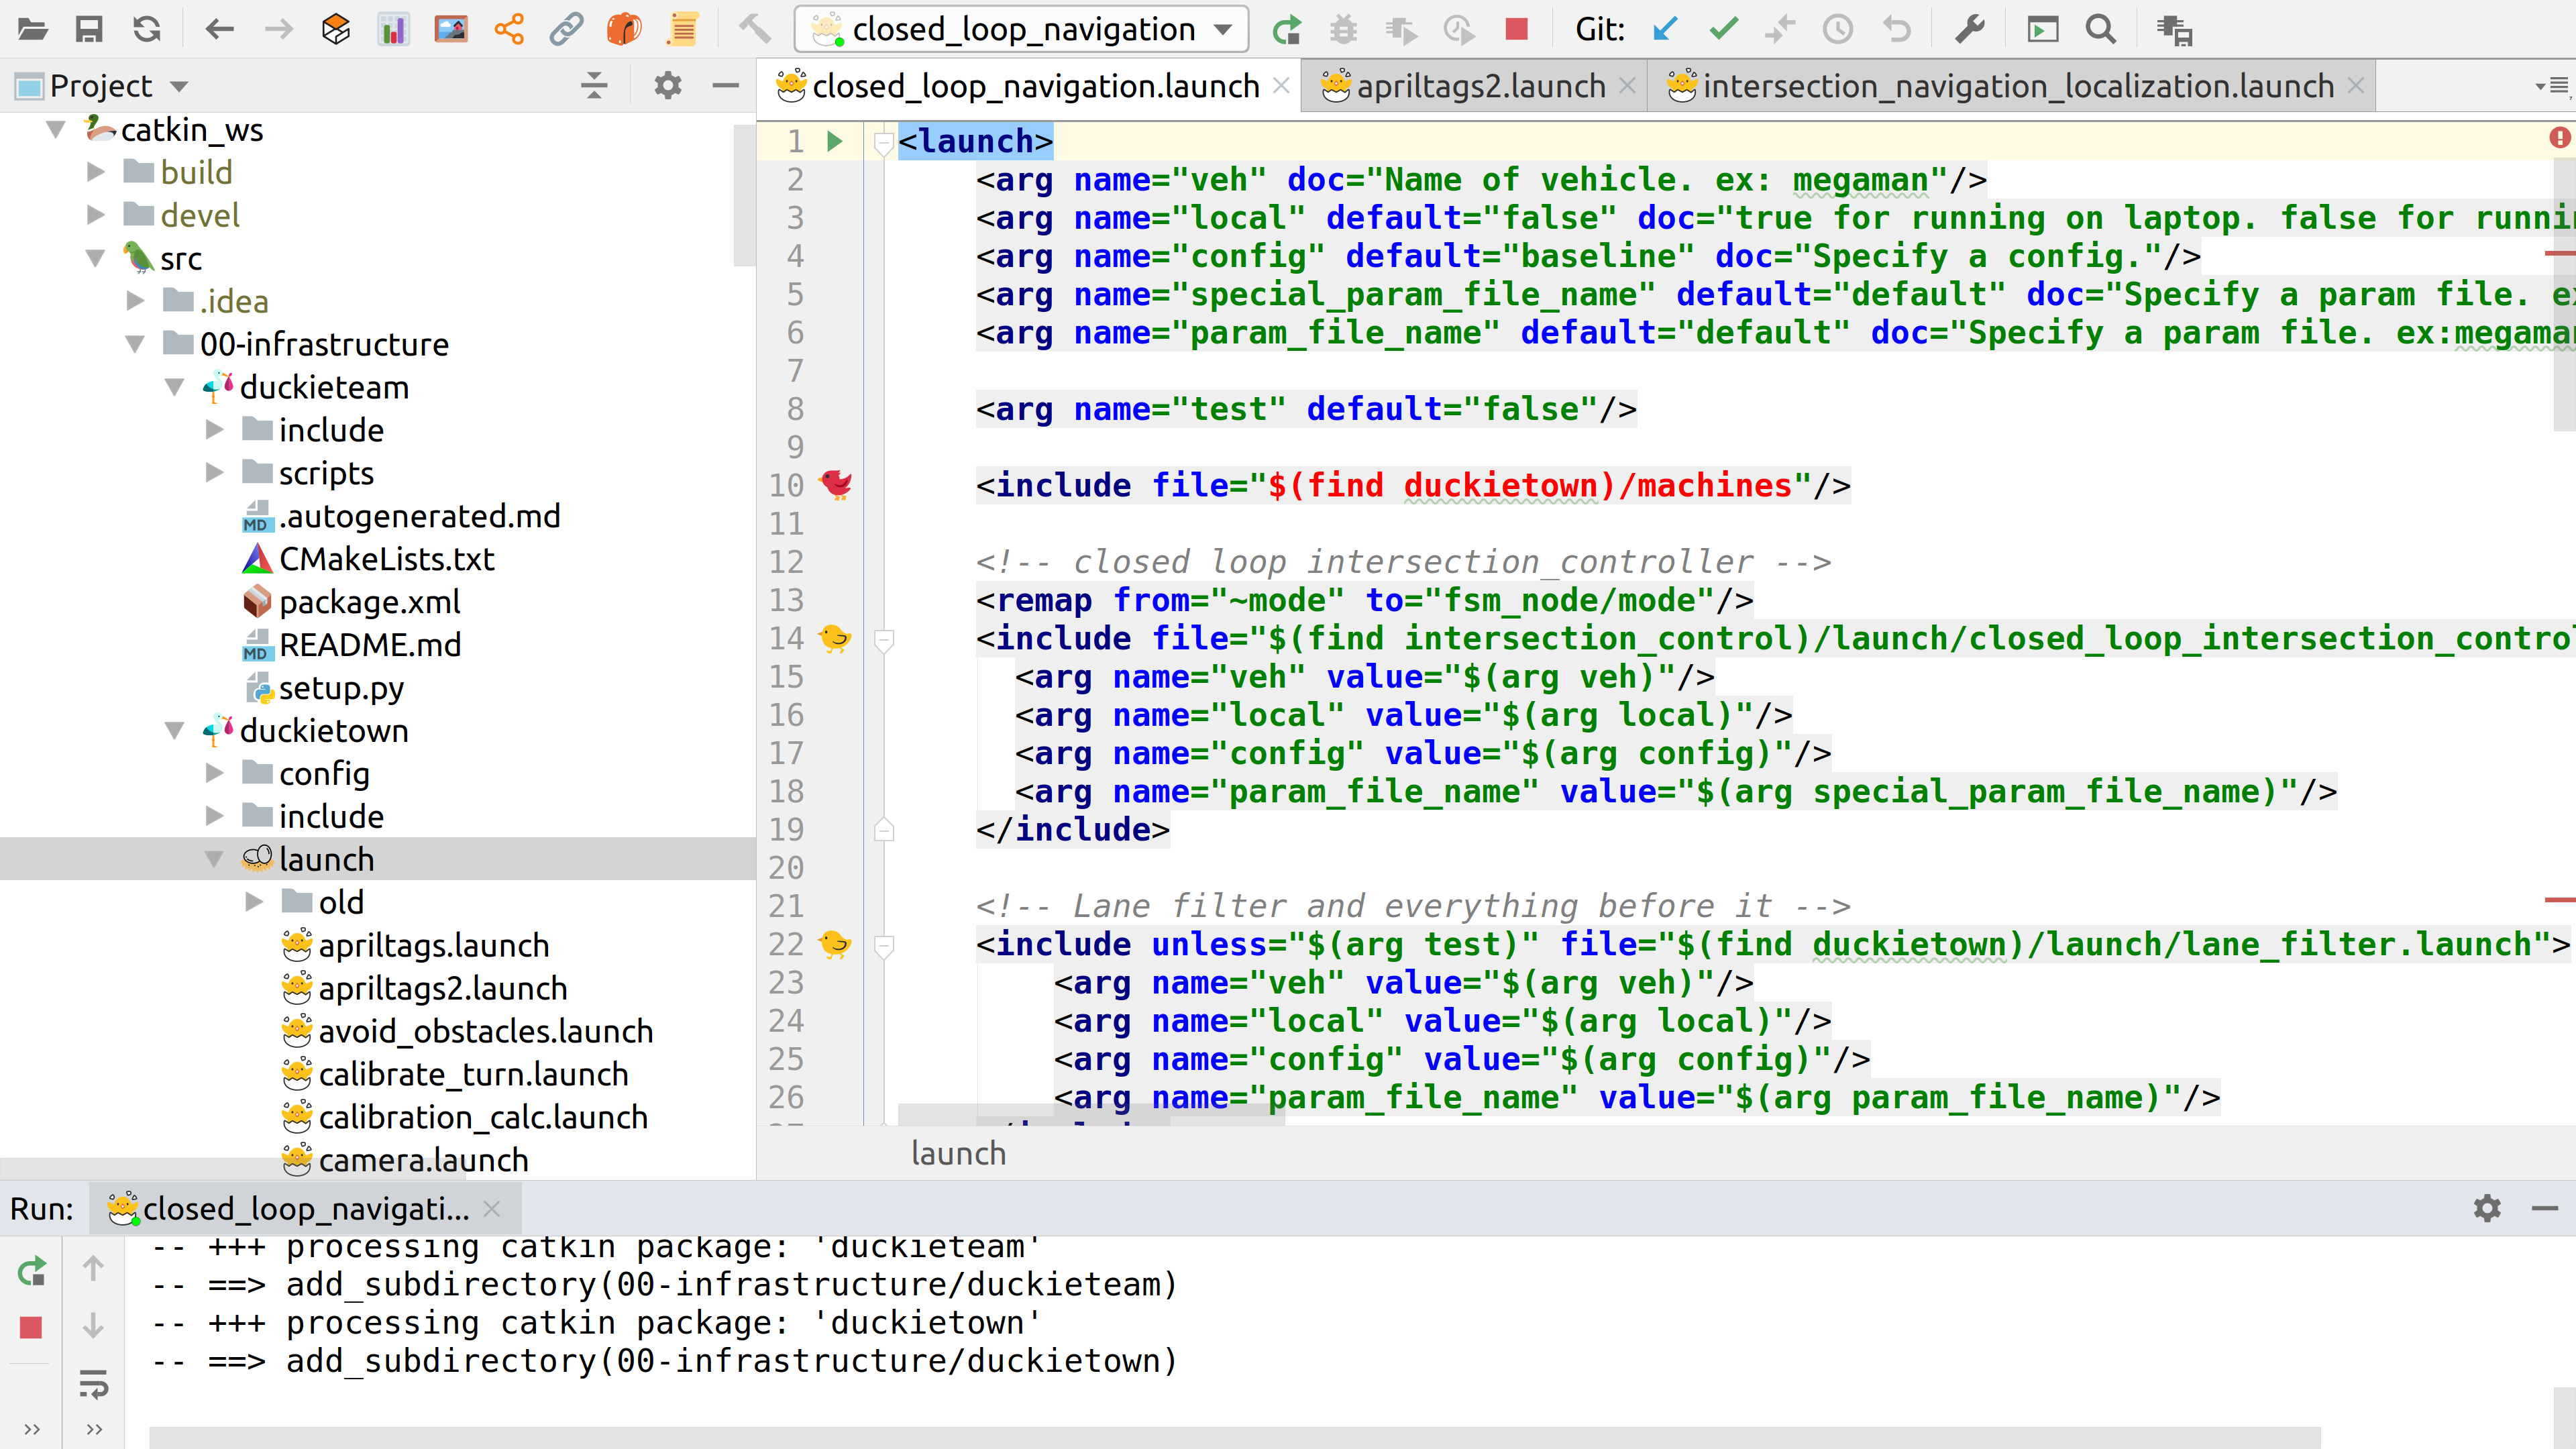
\includegraphics[width=0.90\textwidth]{../figures/hatchery_screenshot.png}}
\caption{Hatchery UI supports syntax highlighting, validation and project navigation.}
\label{fig:hatchery_gui}
\end{figure}
%
\begin{figure}
\centering
\frame{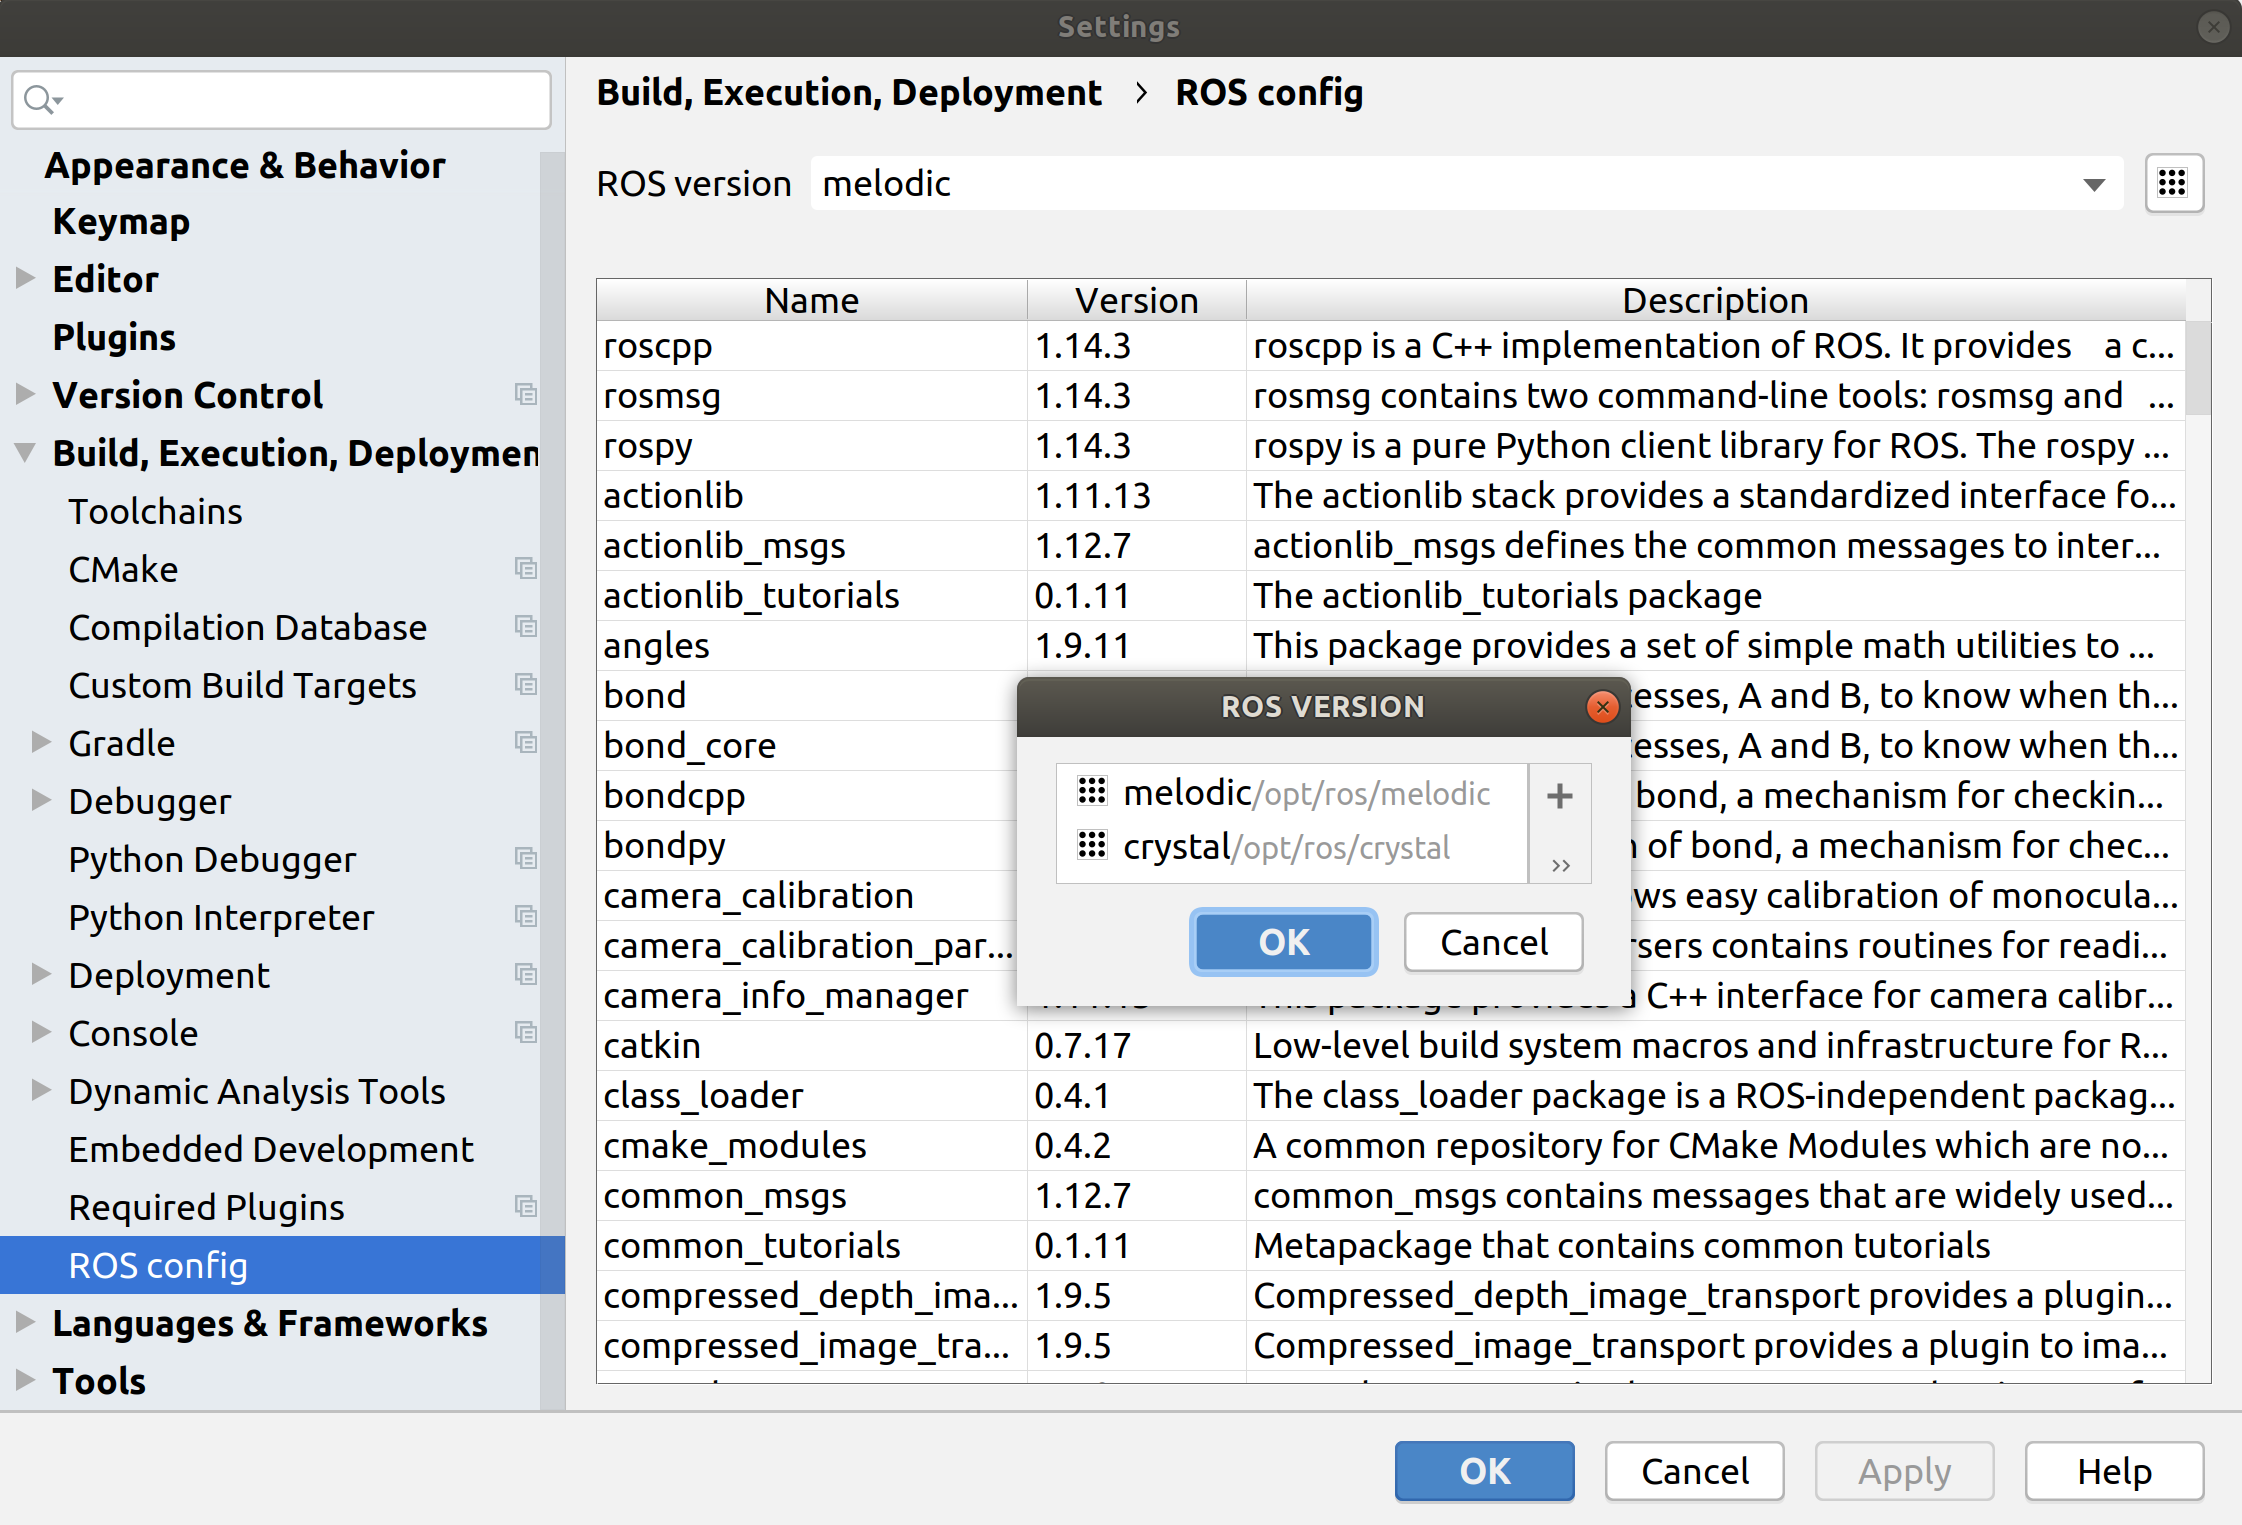
\includegraphics[width=0.90\textwidth]{../figures/ros_settings.png}}
\caption{Detection of local ROS packages. Accessible via: \menu{File > Settings > ROS config}}
\label{fig:ros_settings}
\end{figure}

\section{Ongoing work}

\noindent While it supports many common use cases such as rudimentary code navigation, static analysis and run assistance, Hatchery is currently a work in progress. We are working to expand Hatchery's support for ROS programming in some of the following areas:\vspace{10pt}
%
\begin{itemize}
\item \textbf{Syntax support} -- Highlighting, navigation, autocompletion
\item \textbf{Program analysis} -- Code inspections, intentions, and linting
\item \textbf{Testing support} -- Unit and integration testing, code coverage
\item \textbf{Project creation} -- Project setup and boilerplate code generation
\item \textbf{Dependency management} -- Track installed and missing packages
\item \textbf{Monitoring utils} -- Logging, diagnostics, profiling and visualization
\item \textbf{Crash analytics} -- Enhanced stack traces with source navigation
\item \textbf{Build automation} -- Delta rebuilds, cmake magic, code hotswap
\item \textbf{ROS integration} -- Nodes, topics, services, parameters, graphs
\item \textbf{Duckumentation} -- Usage instructions and supported features
\end{itemize}\vspace{10pt}
%
A more comprehensive list of currently supported and upcoming features are detailed below:\vspace{10pt}
%
\begin{multicols}{2}
\begin{todolist}
\item[\done] ROS Launch (\href{https://wiki.ros.org/roslaunch/XML}{\inline{*.launch}}, \href{https://wiki.ros.org/rostest/Writing}{\inline{*.test}})
\begin{todolist}
\item[\done] Syntax highlighting
\item[\done] Resource references (\inline{\$(find <directory>)...})
\end{todolist}
\item[\done] \href{https://wiki.ros.org/Manifest}{Package manifest (\inline{package.xml})}
\begin{todolist}
\item[\done] Syntax highlighting
\item[\done] \href{https://wiki.ros.org/catkin/package.xml#Dependencies}{Package dependencies} (\inline{<build\_depend>}, \inline{<test\_depend>}, \inline{<run\_depend>})
\end{todolist}
\item[\done] ROS URDF (\inline{*.urdf.xacro})
\begin{todolist}
\item[\done] Syntax highlighting
\item[\done] Resource references (\inline{\$(find <directory>)...})
\end{todolist}
\item[\done] \href{https://wiki.ros.org/Bags/Format}{ROS Bag (\inline{*.bag})}
\begin{todolist}
\item[\done] Syntax highlighting
\end{todolist}
\item[\done] \href{https://wiki.ros.org/msg}{ROS Message (\inline{*.msg})}
\item[\done] \href{https://wiki.ros.org/srv}{ROS Service (\inline{*.srv})}
\item[\done] Implement preliminary project structure and XML support
\item[\done] Write an MVP/POC app that supports file renaming and refactoring
\item[\done] Add support for project templates and skeleton project creation
\item[\done] Add support for deploying a project from the local machine to the remote
\item Add support for monitoring and tracking running code, viewing logs
\begin{todolist}
\item Live logfile tracking
\item Save to local disk
\item Searching the log
\end{todolist}
\item Collect crash dumps and link to the corresponding code points
\begin{todolist}
\item Link stack traces to source code
\item Copy environment info and crash dump to clipboard
\end{todolist}
\item Integration with the \href{https://www.ros.org}{Robot Operating System} (ROS)
\begin{todolist}
\item[\done] ROS 1 support (\href{https://wiki.ros.org/kinetic}{Kinetic Kame} recommended)
\item \href{https://github.com/ros2/ros2/wiki}{ROS 2} support
\item[\done] Managing ROS installations.
\end{todolist}
\item[\done] \href{http://gazebosim.org/}{Gazebo} simulator integration
\item CMake build integration
\item Remote debugging support
\item Docker integration
\begin{todolist}
\item[\done] Basic Docker support
\item Remote host and script support
\item \href{https://hub.docker.com}{Docker Hub} namespace awareness
\item Support for \href{https://platformio.org}{platformio} tooling
\item X11 forwarding and \href{https://wiki.ros.org/rqt}{rqt} support
\end{todolist}
\item Static analysis for \href{https://wiki.ros.org/rospy}{Python API} misuse
\begin{todolist}
\item[\done] Invalid dependency detection
\item Validate \inline{.msg}/\inline{.srv} compatibility
\item ROS nodes and graph analysis via \href{https://wiki.ros.org/rosdep}{\inline{rosdep}}/\href{https://wiki.ros.org/rqt_dep}{\inline{rqt\_dep}}
\end{todolist}
\item \href{https://wiki.ros.org/rqt}{rqt} plugin support
\begin{todolist}
\item[\done] \href{https://wiki.ros.org/rqt_image_view}{\inline{rqt\_img\_view}} - View images
\item[\done] \href{https://wiki.ros.org/rqt_plot}{\inline{rqt\_plot}} - Plot data visually
\item[\done] \href{https://wiki.ros.org/rqt_graph}{\inline{rqt\_graph}} - Graph messages
\item[\done] \href{https://wiki.ros.org/rqt_dep}{\inline{rqt\_dep}} - Visualize dependencies
\item[\done] \href{https://wiki.ros.org/rqt_bag}{\inline{rqt\_bag}} - Replay and edit bag files
\item \href{https://wiki.ros.org/rqt_common_plugins}{rqt\_common} - Other common plugins
\end{todolist}
\end{todolist}
\end{multicols}

\section{Conclusion}

In this chapter we demonstrate the value of IDEs for general purpose software development and present a domain-specific IDE plugin for robotics development, originally developed as a final project in the Duckietown class~\citep{paull2017duckietown}. By using Hatchery, developers can receive assistance when writing, compiling and running ROS applications. The author wishes to express his gratitude to \href{https://github.com/paoloach}{Paolo Achdjian} for contributing several features.


\chapter{Programmation différentiables}\label{ch:kotlingrad}

\setlength{\epigraphwidth}{0.86\textwidth}
\epigraph{Bien que la notation mathématique possède sans aucun doute des règles d'analyse, celles-ci sont assez lâches, parfois contradictoires et rarement clairement énoncées. En raison de leur application à un large éventail de sujets, de leur grammaire stricte et de leur interprétation stricte, les langages de programmation peuvent apporter de nouvelles idées sur la notation mathématique. ''}{\begin{flushright}--Kenneth \citet{iverson1999math}, \href{https://www.cs.trinity.edu/About/The_Courses/cs301/math-for-the-layman/}{\textit{Math pour la Layman}}\end{flushright}}

Dans ce chapitre, nous aborderons la théorie et la mise en œuvre d'un langage spécifique à un domaine et sans danger pour les types, destiné à la différentiation automatique (AD), un algorithme ayant diverses applications dans l'optimisation numérique et l'apprentissage automatique. L'idée clé de l'AD est assez simple. Un petit ensemble d'opérations mathématiques primitives constitue la base de tous les ordinateurs modernes, et en composant ces opérations sur les nombres réels de manière ordonnée, on peut calculer n'importe quelle fonction calculable. Dans l'apprentissage automatique, on nous donne souvent une fonction calculable sous la forme d'un programme qui ne fonctionne pas correctement. Nous voudrions un algorithme pour déterminer comment modifier légèrement l'entrée, afin de produire une sortie plus appropriée.

Un tel algorithme a d'abord été conçu par ~\citet{wengert1964simple}, dont la méthode est connue aujourd'hui sous le nom de AD en mode avancé. Peu de temps après, un certain Richard Bellman a reproduit l'algorithme de Wengert pour estimer numériquement la dynamique orbitale d'un système à deux corps, reconnaissant son potentiel pour, "le traitement de grands systèmes d'équations différentielles qui ne pourraient pas être entrepris autrement" "~\citep{bellman1965wengert}. C'est à peu près à la même époque qu'apparurent les principaux détails de l'algorithme de rétropropagation~\citep{dreyfus1990artificial}. C'est dans la~\citet{linnainmaa1970representation} que l'idée de calculer des dérivées sur des graphiques de calcul a été enregistrée pour la première fois. L'algorithme de Linnaimaa était particulièrement important pour les réseaux de neurones, et est aujourd'hui connu sous le nom de AD en mode inverse. Mais ce n'est qu'en 2010 que les outils logiciels standard~\citep{bergstra2010theano} pour l'AD sont devenus largement disponibles dans l'apprentissage automatique. C'est ici que commence notre voyage.

\section{Différentiation automatique}\label{sec:automatic-differentiation}

Lorsqu'une fonction est dotée d'une certaine entrée, AD nous indique comment modifier l'entrée d'un montant minimal, afin de modifier les sorties au maximum. Supposons qu'on nous donne une fonction $P_k : \mathbb{R}\rightarrow\mathbb{R}$, composée d'une série de fonctions imbriquées, chacune de même type:
%
\begin{equation}
    P_k(x) = \begin{cases} p_1 \circ x = x &\text{if } k=1\\ p_k\circ P_{k-1} \circ x&\text{si } k > 1 \end{cases}
\end{equation}
%
De la règle de la chaîne, on rappelle que le dérivé d'une composition est un produit des dérivés:
%
\begin{equation} \label{eq:sfun_chain_rule}
\frac{dP}{dp_1} = \frac{dp_k}{dp_{k-1}}\frac{dp_{k-1}}{dp_{k-2}}\dots\frac{dp_2}{dp_1}= {\displaystyle \prod_{i=1}^{k-1} \frac{dp_{i+1}}{dp_{i}}}
\end{equation}
%
Étant donné $Q(q_1, \dots, q_m) : \mathbb{R}^m\rightarrow\mathbb{R}$, le \textit{gradient} est une fonction $\nabla Q : \mathbb{R}^m\rightarrow\mathbb{R}\rightarrow\mathbb{R}^m$ définie comme:
%
\begin{equation}
    \nabla Q = \left[ \frac{\partial Q}{\partial q_1}, \dots, \frac{\partial Q}{\partial q_m}\right]
\end{equation}
%
Le \textit{Hessien} est une fonction $\mathbf{H}:\mathbb{R}^m\rightarrow\mathbb{R}\rightarrow\mathbb{R}^{m\times m}$ renvoyant une matrice de partiels de second ordre:
%
\begin{equation}
    \mathbf{H}(Q) = \begin{bmatrix}{\dfrac {\partial ^{2}Q}{\partial x_{1}^{2}}}&{\dfrac {\partial ^{2}Q}{\partial x_{1}\,\partial x_{2}}}&\cdots &{\dfrac {\partial ^{2}Q}{\partial x_{1}\,\partial x_{m}}}\\[2.2ex]{\dfrac {\partial ^{2}Q}{\partial x_{2}\,\partial x_{1}}}&{\dfrac {\partial ^{2}Q}{\partial x_{2}^{2}}}&\cdots &{\dfrac {\partial ^{2}Q}{\partial x_{2}\,\partial x_{m}}}\\[2.2ex]\vdots &\vdots &\ddots &\vdots \\[2.2ex]{\dfrac {\partial ^{2}Q}{\partial x_{m}\,\partial x_{1}}}&{\dfrac {\partial ^{2}Q}{\partial x_{m}\,\partial x_{2}}}&\cdots &{\dfrac {\partial ^{2}Q}{\partial x_{m}^{2}}}\end{bmatrix}
\end{equation}
%
Pour les fonctions vectorielles $\mathbf{f} : \mathbb{R}^m\rightarrow\mathbb{R}^n$, le \textit{Jacobien}, $\mathcal{J}_{\mathbf{f}} : \mathbb{R}^m\rightarrow\mathbb{R}^n\fourchette droite\mathbb{R}^{n \times m}$ est défini comme:
%
\begin{equation}
    \mathcal{J}_{\mathbf{f}} =
    \begin{bmatrix}
        \dfrac{\partial \mathbf{f}}{\partial x_1} & \cdots & \dfrac{\partial \mathbf{f}}{\partial x_m}
    \end{bmatrix} =
    \begin{bmatrix}
        \dfrac{\partial f_1}{\partial x_1} & \cdots & \dfrac{\partial f_1}{\partial x_m}\\
        \vdots & \ddots & \vdots\\
        \dfrac{\partial f_n}{\partial x_1} & \cdots & \dfrac{\partial f_n}{\partial x_m}
    \end{bmatrix} =
    \begin{bmatrix}
        \nabla f_1 \\
        \vdots \\
        \nabla f_m
    \end{bmatrix}
\end{equation}
%
Pour les fonctions scalaires, la transposition du Hessien est équivalente au Jacobien du gradient:
%
\begin{equation}
    \mathbf{H}(Q)^\intercal = \mathcal{J}_\mathbf{q}(\nabla Q)
\end{equation}
%
Pour une fonction vectorielle $\mathbf{P}_k(\mathbf{x}) : \mathbb{R}^m\rightarrow\mathbb{R}^n$, la règle de la chaîne de \autoref{eq:sfun_chain_rule} s'applique toujours:
%
\begin{equation} \label{eq:vfun_chain_rule}
\mathcal{J}_\mathbf{P_k} = \displaystyle \prod_{i=1}^{k} \mathcal{J}_{p_i} = \underbrace{\bigg(\Big((\mathcal{J}_{p_k} \mathcal{J}_{p_{k-1}}) \dots \mathcal{J}_{p_2}\Big) \mathcal{J}_{p_1}\bigg)}_{\textit{``Reverse accumulation''}} = \underbrace{\bigg(\mathcal{J}_{p_k} \Big(\mathcal{J}_{p_{k-1}} \dots (\mathcal{J}_{p_2} \mathcal{J}_{p_1})\Big)\bigg)}_{\textit{``Forward accumulation''}}
\end{equation}
%
Pour l'exhaustivité, mais rarement utilisé dans la pratique, est le deuxième ordre partiel pour les fonctions vectorielles:
%
\begin{equation}
    \mathbf{H} (\mathbf {f} )=[\mathbf {H} (f_{1}), \mathbf {H} (f_{2}), \dots, \mathbf {H} (f_{n})]
\end{equation}
%
Nous pouvons utiliser ces outils pour calculer la direction afin d'ajuster les entrées d'une fonction calculable, afin de modifier au maximum la sortie de cette fonction, c'est-à-dire la direction de la descente la plus raide.

\noindent Parfois, une fonction a la propriété qu'étant donné une entrée $a$, peu importe comment $a$ est modifié, la sortie reste la même. Nous disons que de telles fonctions ont une pente nulle pour cette entrée.
%
\begin{equation}
    (\nabla F)(a) \approx \mathbf{0}
\end{equation}
%
Le coût du calcul du Hessois, $\mathbf{H}$ est approximativement quadratique~\citep{griewank1993some} par rapport au nombre de variables indépendantes sous différentiation. Si $\mathbf{H}(a)$ est tractable à calculer et inversible, nous pourrions utiliser le test de la dérivée seconde partie pour déterminer que:\\
%
\begin{enumerate}
\item Si toutes les valeurs propres de $\mathbf{H}(a)$ sont positives, $a$ est un minimum local
\item Si toutes les valeurs propres de $\mathbf{H}(a)$ sont négatives, $a$ est un maximum local
\item Si $\mathbf{H}$ contient un mélange de valeurs propres positives et négatives, $a$ est un \textit{saddle point}\\
\end{enumerate}
%
Pour certaines classes de fonctions calculables, de petites modifications de l'entrée produiront une variation soudaine et importante de la sortie. Nous disons que ces fonctions sont non différentiables.
%
\begin{equation}
    ||(\nabla F)(a)|| \approx \pm \infty
\end{equation}
%
La question de savoir si des fonctions non différentiables existent dans le monde réel est ouverte~\citep{buniy2005hilbert}. À l'échelle physique (10nm) et temporelle (10ns) actuelle de l'informatique moderne, il n'existe pas de telles fonctions, mais la plupart des ordinateurs modernes sont incapables de rendre compte de la valeur réelle de leurs fonctions à valeur binaire. À toutes fins utiles, les programmes mis en œuvre par la plupart des ordinateurs physiques sont des relations discrètes. Néanmoins, les programmes discrets sont capables d'approcher des fonctions bornées sur $\mathbb{R}^m$ avec une précision arbitraire si l'on tient compte du temps et de l'espace. Pour la plupart des applications, une approximation de faible précision (32-64 bits) est suffisante.

Il existe au cœur de l'apprentissage automatique un théorème qui énonce une famille simple de fonctions, qui calculent une somme pondérée d'une fonction non linéaire $\varphi : \mathbb{R} \rightarrow \mathbb{R}$ composée d'une fonction linéaire $\theta^\intercal \mathbf{x} + b$, peut approximer toute fonction bornée $\mathbb{R}^m\rightarrow\mathbb{R}$ à une précision arbitraire. Plus précisément, le théorème d'approximation universel~\citep{hornik1989multilayer} indique que pour toutes les fonctions continues à valeur réelle $f : C(\mathbb{I}_m)$, où $\mathbb{I}_m = [0, 1]^m \rightarrow [0, 1]$, il existe un $\hat f : \mathbb{R}^m \times \mathbb{R}^{n \times m} \rightarrow \mathbb{R}$, paramétrée par $\Theta \in \mathbb{R}^{n \times m}$, en prenant une entrée $\mathbf x \in [0, 1]^m$ et des constantes $n \in \mathbb{N}, \mathbf{\beta} \in \mathbb{R}^n, \mathbf{b} \in \mathbb{R}^n, \epsilon \in \mathbb{R}^+$ tel que la déclaration suivante tient:
%
\begin{equation}
    \begin{split}
        \hat{f}(\mathbf{x}; \Theta) = \mathbf{\beta}^\intercal \varphi_{\odot} \left(\Theta^\intercal \mathbf{x} + \mathbf{b}\right) \\
        \forall \mathbf{x} \in \mathbb{I}_m, \ | \hat f( \mathbf{x} ) - f ( \mathbf{x} ) | < \epsilon
    \end{split}
\end{equation}
%
$\varphi_{\odot}$ indique une fonction non linéaire $\varphi$ appliquée par élément au vecteur. Ce théorème nous dit seulement que $\Theta$ existe, mais ne nous dit pas comment le trouver et ne fixe pas de limite supérieure à la constante $n$, ce qui limite quelque peu son applicabilité pratique. Mais pour des raisons encore mal comprises, les résultats empiriques suggèrent qu'il est possible d'approximer de nombreuses fonctions naturelles en un nombre relativement court d'étapes en composant plusieurs \textit{couches} de $\Theta^\intercal \mathbf{x} + \mathbf{b}$ et $\varphi$ en alternance, et en mettant à jour chaque $\Theta$ en utilisant une procédure basée sur la descente de la pente. Le modèle qui en résulte peut être exprimé comme suit\footnote{La notation ci-dessous suppose une certaine familiarité avec le curry et l'application de fonctions partielles, dans lesquelles $\mathbf{\hat P}: \mathbb{R}^m \rightarrow \mathbb{R}^n \equiv \underbrace{\mathbb R \rightarrow \ldots \rightarrow \mathbb R}_{m}\rightarrow \mathbb{R}^n$. Pour plus de détails, voir \citet{schonfinkel1924bausteine, curry1958combinatory} et al.},
%
\begin{equation} \label{eq:recursive_parametric_eq}
\mathbf{\hat P}_k(\mathbf{x}; \bm\Theta) = \begin{cases} \mathbf{\hat p}_1(\Theta_1)\circ\mathbf{x} &\text{si } k=1\\ \mathbf{\hat p}_k(\Theta_k)\circ \mathbf{\hat P}_{k-1}(\bm\Theta_{[1, k-1]})\circ\mathbf{x}&\text{si } k > 1 \end{cases} \\
\end{equation}
%
$\bm\Theta = \{\Theta_1, \dots, \Theta_k\}$ sont des paramètres libres et $\mathbf{x} \in \mathbb{R}^m$ est une entrée unique. Pour obtenir approximativement $\mathbf{P}(\mathbf x)$, il faut obtenir $\mathbf{X} = \{\mathbf{x}^{(0)}, \dots, \mathbf{x}^{(z)}\}, \mathbf{Y} = \{\mathbf{y}^{(0)} = \mathbf{P}(\mathbf{x}^{(0)}), \dots, \mathbf{y}^{(z)} = \mathbf{P}(\mathbf{x}^{(z)})\}$ en quantité aussi grande et variée que possible et répéter la procédure suivante jusqu'à ce que $\bm\Theta$ converge:
%
\begin{equation} \label{eq:stochastic_grad_descent}
\bm\Theta \leftarrow \bm\Theta - \alpha\frac{1}{z}\nabla_{\bm\Theta} \sum_{i=1}^z\mathcal{L}\big(\mathbf{\hat P}_k(\mathbf{x}^{(i)}; \bm\Theta), \mathbf{y}^{(i)}\big)
\end{equation}
%
Dans le cas général, nous pouvons résoudre le gradient en utilisant \autoref{eq:vfun_chain_rule}. Pour les $\mathcal{L}$ les plus courants, la complexité de cette procédure est linéaire avec $z$. Comme $z$ peut être assez important en pratique, et comme l'obtention du gradient exact n'est pas importante, nous utilisons une variante stochastique en rééchantillonnant un \textit{minibatch} $\mathbf{X}', \mathbf{Y}'$ composé de paires $\mathbf{x}^{(i)}, \mathbf{y}^{(i)}$ pour $i \sim \{0, \dots, z\}$ sans remplacement à chaque étape de mise à jour. C'est légèrement plus bruyant, mais fonctionne beaucoup plus rapidement.

\section{Programmation différentiable}\label{sec:differentiable-programming}

\begin{figure}
    \centering
    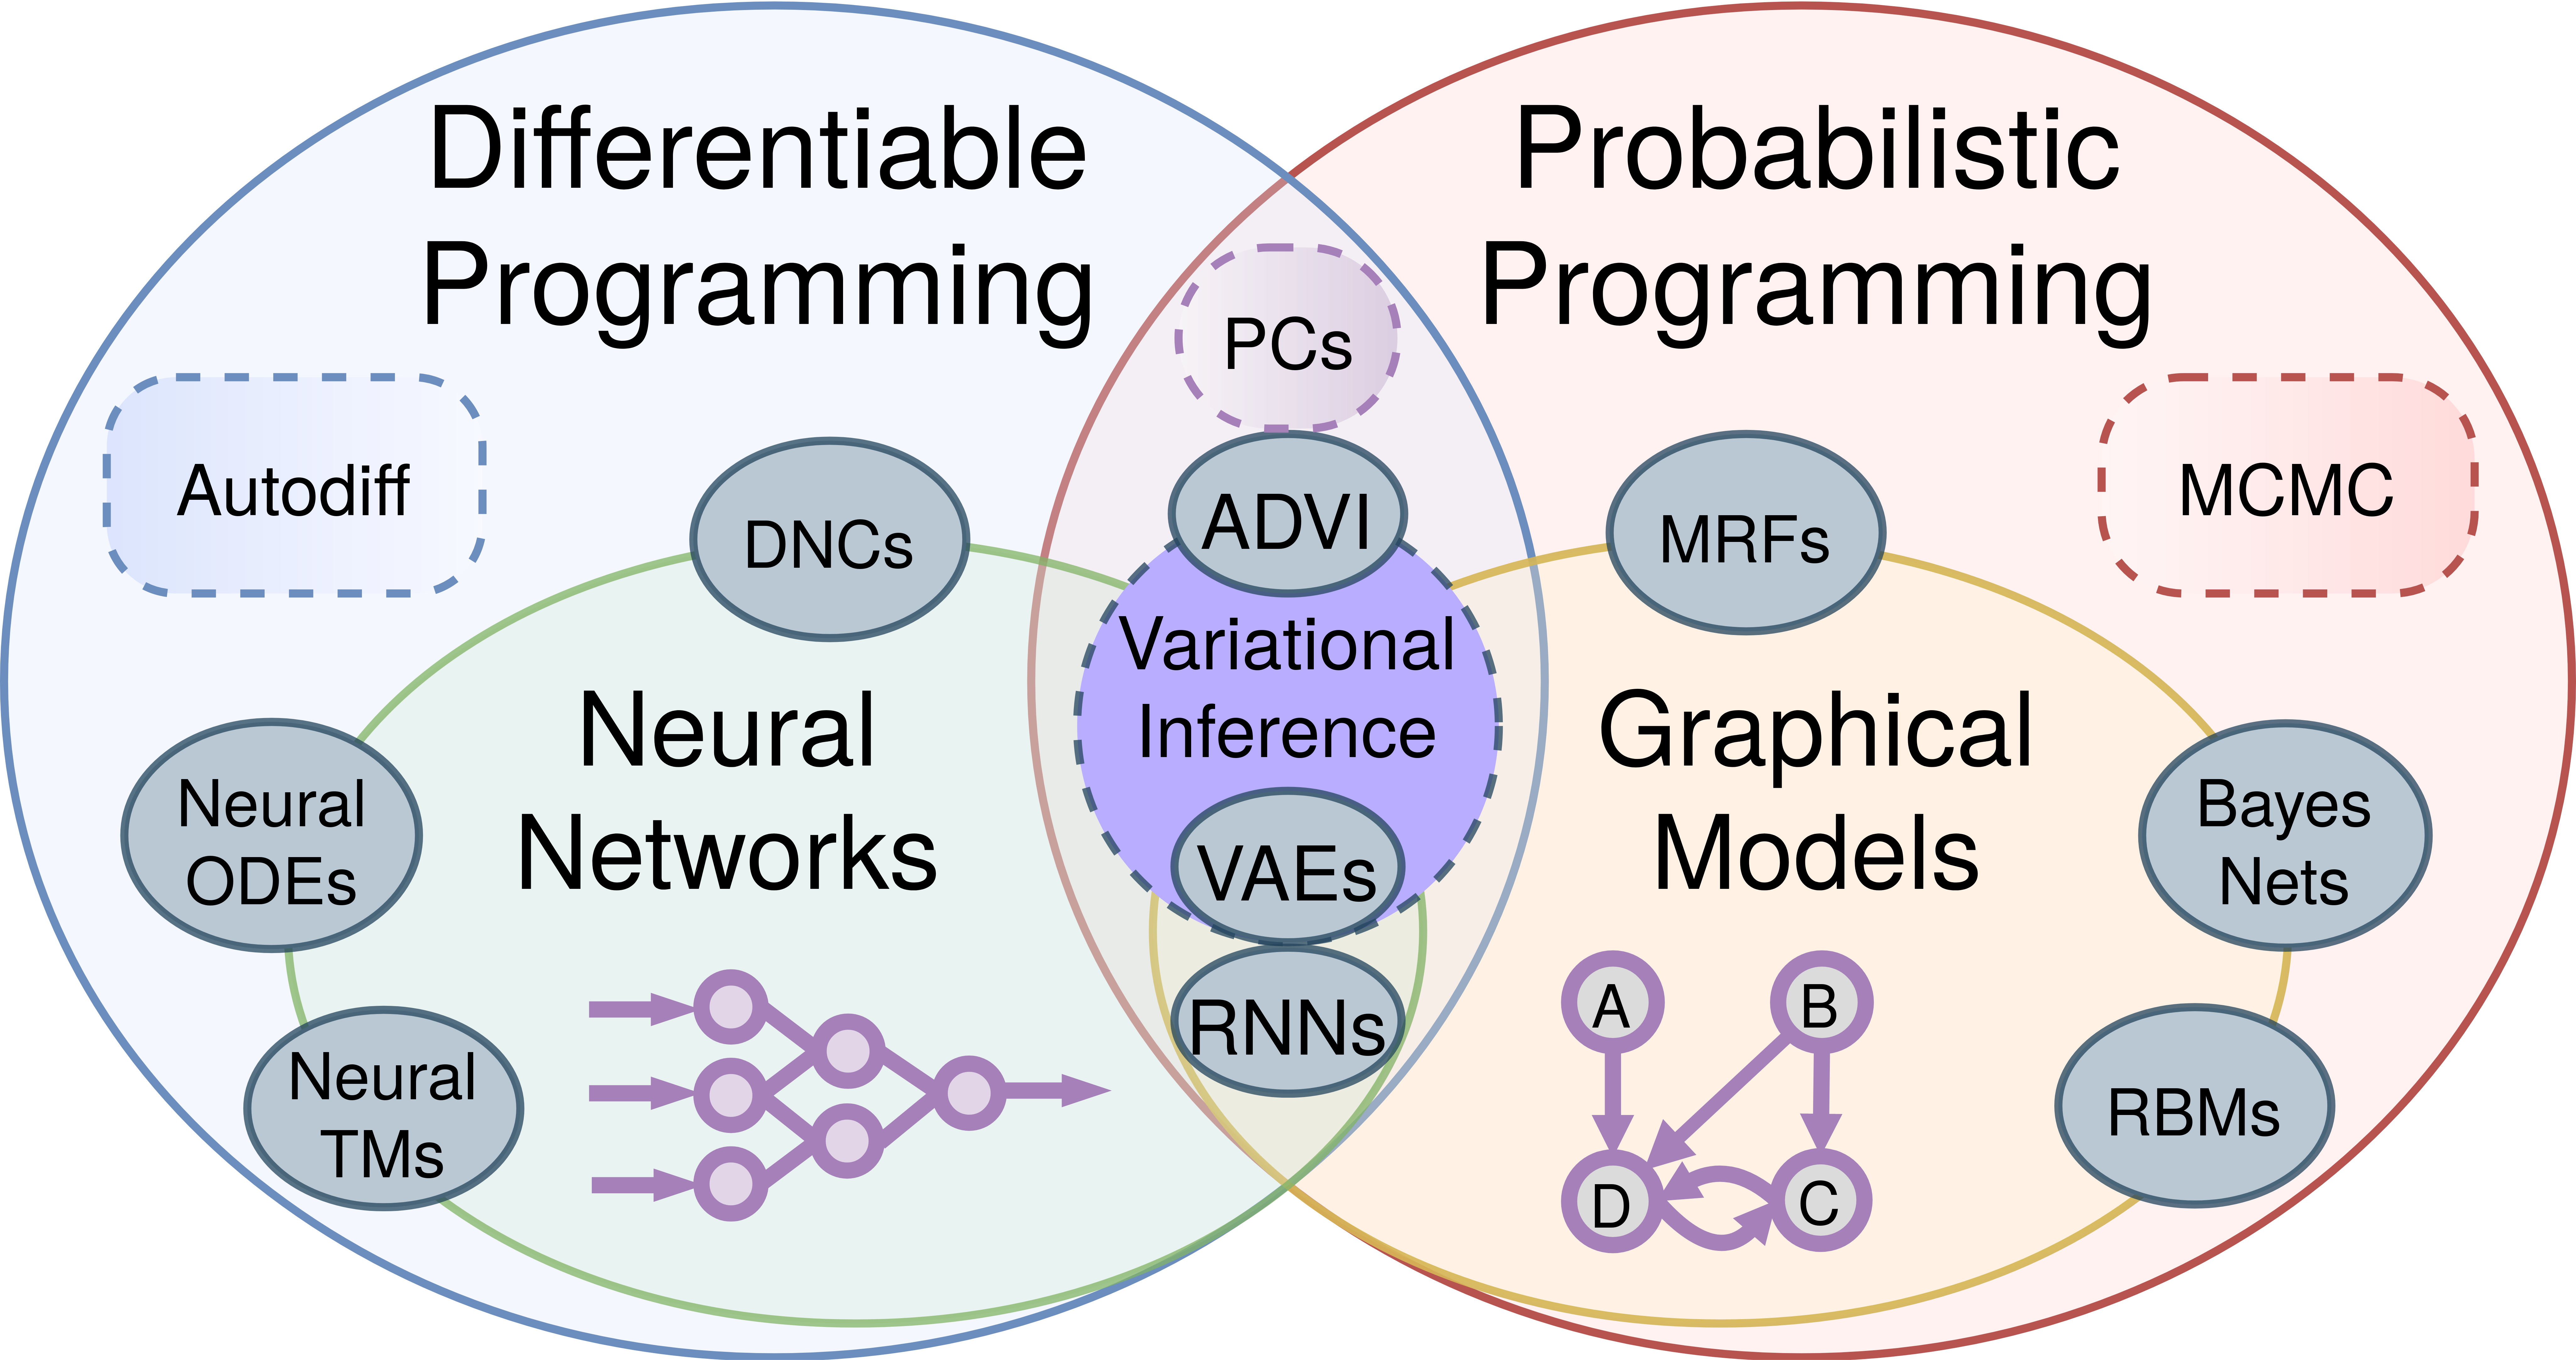
\includegraphics[width=0.90\textwidth]{../figures/diff_prob_prog.png}
    \caption{\textit{Programmation différentiable} comprend les réseaux de neurones, mais plus largement, les programmes arbitraires qui utilisent l'optimisation par gradient pour se rapprocher d'une fonction de perte. \textit{Programmation probabiliste}~\citep{tristan2014augur, carpenter2017stan, gorinova2018slicstan} est une généralisation des modèles graphiques probabilistes qui utilise les méthodes de Monte Carlo (MC) pour approcher une fonction de densité.}
    \label{fig:diff_prob_prog}
\end{figure}

La renaissance de l'apprentissage profond moderne est largement attribuée aux progrès réalisés dans trois domaines de recherche : les algorithmes, les données et le matériel. Parmi les algorithmes, la plupart des recherches ont porté sur les architectures d'apprentissage profond et l'apprentissage par représentation. Le rôle que la différentiation automatique (DA) a joué pour faciliter la mise en œuvre de ces idées est sans doute tout aussi important. Avant l'avènement des bibliothèques AD à usage général telles que \href{http://deeplearning.net/software/theano/}{Theano}, \href{https://pytorch.org/}{PyTorch} et \href{https://tensorflow.org/}{TensorFlow}, les gradients devaient être dérivés manuellement. L'adoption généralisée des logiciels de DA a simplifié et accéléré le rythme de l'apprentissage automatique basé sur les gradients, permettant aux chercheurs de construire des architectures de réseau plus profondes et de nouvelles représentations d'apprentissage. Certaines de ces idées ont à leur tour servi de base à de nouvelles méthodes de DA, qui continue d'être un \href{http://www.autodiff.org}{domaine actif} de la recherche dans les communautés du langage de programmation et du calcul scientifique.

Un aspect clé du paradigme connexionniste est la descente en gradient d'une fonction de perte statistique définie sur un réseau neuronal par rapport à ses paramètres libres. Pour que la descente de gradient fonctionne, la représentation doit pouvoir être différenciée presque partout. Cependant, de nombreuses représentations ne sont pas différentiables dans leur domaine naturel. Par exemple, la structure du langage écrit n'est pas facilement différentiable, car de petites modifications de la forme symbolique d'un mot peuvent entraîner des changements soudains de sa sémantique~\citep{vanmerrienboer2018phd}. L'un des principaux enseignements de l'apprentissage de la représentation est que de nombreux types de données discrètes peuvent être mis en correspondance dans un espace latent plus lisse. Par exemple, si nous représentons les mots comme un vecteur de nombres réels, $\mathbb R^N$, alors il est possible d'apprendre une correspondance des mots à $\mathbb R^N$ de sorte que les relations sémantiques entre les mots (telles que définies par leur co-occurrence statistique dans les grands corpus) sont géométriquement préservées dans l'espace vectoriel~\citep{pennington2014glove} -- les mots ayant une signification similaire sont associés à des vecteurs similaires. De nombreuses classes de problèmes discrets peuvent être relâchées pour devenir des substituts continus en apprenant de telles représentations, ou \textit{embeddings} de manière non supervisée, ou semi-supervisée.

À peu près à la même époque, la communauté d'apprentissage profond a réalisé que la différentiation stricte n'était peut-être pas si importante tout au long du processus. Il a été démontré en pratique que les ordinateurs utilisant l'arithmétique à virgule flottante 8 bits~\citep{wang2018training} et l'arithmétique des nombres entiers~\citep{wu2018training, jacob2018quantization} sont capables de former des réseaux de neurones sans sacrifier les performances. Des hypothèses fortes comme la continuité de Lipschitz et la douceur $\beta$ autrefois considérées comme indispensables pour l'apprentissage par gradient peuvent être assouplies, tant que le bruit introduit par la quantification est négligeable par rapport aux méthodes de gradient stochastique. Avec le recul, cela aurait dû être moins surprenant, puisque tous les ordinateurs numériques utilisent de toute façon des représentations discrètes et ont été capables de former des réseaux neuronaux pendant près d'un demi-siècle. Cela suggère qu'une différentiation stricte n'était pas aussi importante que d'avoir une bonne métrique. Tant que la surface de perte permet l'apprentissage de la métrique, la descente de gradient est étonnamment résistante à la quantification.

Au fur et à mesure que l'apprentissage profond développait de nouvelles applications, les chercheurs ont observé que les réseaux neuronaux faisaient partie d'une classe plus large d'architectures différentiables qui pouvaient être structurées d'une manière similaire aux programmes informatiques. D'où le terme \textit{programmation différentiable}~\citep{olah2015neural, baydin2016differentiable, plotkin2018some} (DP) est né. Aujourd'hui, la DP a de nombreuses applications, des techniques classiques de CS comme le classement et le tri~\citep{cuturi2019differentiable, blondel2020fast}, au pliage des protéines~\citep{alquraishi2018end}, aux moteurs physiques~\citep{hu2019difftaichi, de2018end, degrave2016differentiable} et au rendu graphique~\citep{loper2014opendr} au meta-learning~\citep{liu2018darts, chandra2019gradient}. Ces applications ont toutes des paramètres qui peuvent être appris via la descente de gradient. Pour apprendre des relations discrètes sans intégration ad hoc, des techniques supplémentaires (\autoref{sec:future-work}), telles que la programmation probabiliste, sont probablement nécessaires. Divers langages de programmation probabiliste, dont Stan~\citep{carpenter2017stan}, Pyro~\citep{bingham2019pyro}, PyMC4~\citep{kochurov2019pymc4} et autres, ont également vu le jour. Comme le montre \autoref{fig:diff_prob_prog}, ces deux domaines ont bénéficié de nombreuses collaborations fructueuses ces dernières années.

\section{Langages statiques et dynamiques}

La plupart des programmes d'apprentissage automatique et de calcul scientifique sont écrits dans des langages dynamiques, tels que Python. En revanche, la plupart des industries utilisent des langages à caractères statiques~\citep{github}. Selon certaines études, les erreurs liées aux types représentent plus de 15\% des bogues logiciels~\citep{gao2017type}. Bien que la causalité entre la défectuosité et le typage statique n'ait pas été établie de manière concluante, les langages à caractères dynamiques sont rarement utilisés pour la construction de systèmes critiques pour la sécurité, et la majorité des applications robotiques~\citep{guenther2018serious} sont écrites dans des langages à caractères statiques.

Le typage statique élimine une large classe d'erreurs d'exécution, permettant aux développeurs et aux outils de raisonner plus soigneusement sur le comportement des programmes sans avoir besoin de les exécuter. En plus d'une validation syntaxique renforcée pour la programmation générale, une bibliothèque bien conçue dans un langage fortement typé peut éliminer les erreurs spécifiques à un domaine liées à une mauvaise utilisation de l'API qui, autrement, nécessiteraient une documentation et des échantillons de code pour les éviter, ce qui améliore la convivialité et réduit la maintenance. En outre, les systèmes de types forts permettent aux EDI de fournir des outils d'analyse statique plus précis, tels que l'autocomplétion pertinente, la navigation dans le code source et la détection plus précoce des erreurs d'exécution.

Une objection courante à l'utilisation de langages à caractères forts est la charge supplémentaire que représente l'annotation manuelle des types~\citep{ore2018assessing}. Alors que les premiers langages à sécurité typographique comme C++ et Java exigeaient des programmeurs qu'ils annotent de manière exhaustive les déclarations de fonctions et de variables, avec une utilisation judicieuse de l'inférence de type dans les langages modernes comme Kotlin, Scala, Rust et autres, la plupart des signatures de type peuvent être omises sans risque et facilement récupérées dans le contexte environnant. L'inférence de type permet aux langues modernes d'offrir la brièveté des langues à typographie dynamique avec la sécurité d'une vérification statique des types.

\section{Langages impératifs et fonctionnels}

La plupart des programmes sont aujourd'hui écrits dans le style impératif, en raison de la prédominance de la machine de Turing et de l'architecture von Neumann~\citep{backus2007can}. $\lambda$-calculus fournit une note de bas de page équivalente {en ce sens que la machine de Turing et $\lambda$-calculus sont tous deux des langages de Turing complets.} pour le calcul, ce qui, selon nous, est une notation plus appropriée pour exprimer des fonctions mathématiques et calculer leurs dérivés. Dans la programmation impérative, le seul but de l'utilisation d'une fonction est de lui transmettre des valeurs, et il n'y a pas moyen de se référer à une fonction sans le faire. Ce qui est plus troublant dans le cas de la DA, c'est que les programmes impératifs ont un état mutable, ce qui nécessite de prendre des précautions supplémentaires lors du calcul de leurs dérivées.

La notion mathématique de composition des fonctions est un citoyen de premier ordre en matière de programmation fonctionnelle. Tout comme en calcul, pour prendre la dérivée d'un programme composé avec un autre programme, on applique simplement la règle de la chaîne (\autoref{sec:automatic-differentiation}). Comme il n'y a pas d'état mutable dans la PF, aucune structure de données exotiques ou d'astuces de compilation n'est nécessaire.

Par exemple, considérons la fonction vectorielle $f(l_1, l_2) = l_1 \cdot l_2$, vue dans \autoref{fig:fp_vs_ip}. Les programmes impératifs, en permettant la mutation, détruisent effectivement les informations intermédiaires. Afin de récupérer le graphique de calcul pour la MA en mode inversé, nous devons soit passer outre l'opérateur d'affectation, soit utiliser une bande pour stocker les valeurs intermédiaires. Dans la programmation fonctionnelle pure, les variables mutables n'existent pas, ce qui nous facilite grandement la vie.

\begin{figure}[t]
    \centering
    \begin{tabular}{|l|l|}
        \hline
        Impératif & Fonctionnel \\
        \hline
{\begin{lstlisting}[style=barelisting, linewidth=5.7cm, numbers=left]
fun dot(l1, l2) {
    if (len(l1) != len(l2))
        return error
    var sum = 0
    for(i in 0 to len(l1))
        sum += l1[i] * l2[i]
    return sum
}
\end{lstlisting}}
        &
{\begin{lstlisting}[style=barelisting, linewidth=6.5cm, numbers=none]
fun dot(l1, l2) {
    return if (len(l1) != len(l2))
        error
    else if (len(l1) == 0) 0
    else
        head(l1) * head(l2) +
        dot(tail(l1), tail(l2))
}
\end{lstlisting}}
        \\
        \hline
    \end{tabular}
    \caption{Deux programmes équivalents pour l'équation $f(l_1, l_2) = l_1 \cdot l_2$.}
    \label{fig:fp_vs_ip}
\end{figure}

La programmation fonctionnelle permet à Kotlin$\nabla$ d'utiliser la même abstraction pour représenter les fonctions mathématiques et les fonctions de programmation. Toutes les fonctions de Kotlin$\nabla$ sont des fonctions pures, composées d'expressions formant un graphe de flux de données (DFG). Une expression est simplement une \inline{Function}, qui n'est évaluée que lorsqu'elle est invoquée avec des valeurs numériques, par exemple \inline{z(0, 0)}. De cette manière, Kotlin$\nabla$ est similaire à d'autres cadres basés sur des graphes comme \href{http://deeplearning.net/software/theano/extending/graphstructures.html}{Theano} et \href{https://www.tensorflow.org/guide/graphs}{TensorFlow}.

\section{Kotlin}\label{sec:kotlin}

Lors de la programmation dans un langage à caractères statiques, une question courante que l'on peut poser au compilateur est la suivante : "En donnant une valeur, \inline{x}, peut-on assigner \inline{x} à une variable de type \inline{Y}? (par exemple, vérification du type \inline{x instanceof Y}) En Java, cette question s'avère être \href{http://io.livecode.ch/learn/namin/unsound}{ill-posed}~\citep{amin2016java} et indécidable~\citep{grigore2017java} dans le cas général. Il est possible de construire un programme Java dans lequel la réponse est "oui" indépendamment de \inline{Y}, ou pour lequel une réponse ne peut pas toujours être déterminée en temps fini. L'indécidabilité n'est pas nécessairement un obstacle, mais le manque de solidité de Java est plus critique et la manière de le corriger n'est pas claire, même si cela se produit rarement dans la pratique.

Kotlin est un langage de type statique qui convient bien à la construction d'applications multiplateformes, avec un support de compilation pour JVM, JavaScript et des cibles natives. Contrairement à la plupart des langages de programmation, Kotlin a été conçu dès le départ avec le support de l'IDE, et a gagné une certaine notoriété dans l'écosystème JVM grâce à son ergonomie. Le système de types de Kotlin~\citep{tate2013mixed} est strictement \href{https://kotlinlang.org/docs/reference/generics.html#variance}{moins expressif}, mais totalement interopérable avec celui de Java. On ignore si les mêmes problèmes qui affectent le système de types de Java sont présents dans Kotlin, mais l'interopérabilité avec Java a élargi son adoption et reste un élément clé de la convivialité du langage.

Dans ce travail, nous utilisons plusieurs caractéristiques du langage propres à Kotlin, telles que les fonctions de première classe (\autoref{sec:first-class-functions}), les fonctions d'extension (\autoref{sec:extension-functions}), la surcharge des opérateurs (\autoref{sec:operator-overloading}) et les types de données algébriques (\autoref{sec:adts}). En outre, nous utilisons largement le \href{https://kotlinlang.org/docs/reference/type-safe-builders.html}{support SDL} de Kotlin pour mettre en œuvre la programmation de tableaux à sécurité de forme. Ensemble, ces caractéristiques de langage fournissent une plate-forme concise, flexible et sans risque de type pour la programmation mathématique.

\section{Kotlin\textorpdfstring{$\nabla$}}\label{sec:kotlingrad}

Des travaux antérieurs ont démontré la possibilité d'encoder un langage déterministe sans contexte (DCF) dans le système de type Java comme \textit{interface fluide}~\citep{gil2016formal, nakamaru2017silverchain}. Ce résultat a été renforcé pour prouver que le système de types de Java est complet de Turing (TC)~\citep{grigore2017java}, ce qui nous permet d'effectuer des contrôles de forme et des inférences sur des programmes de tableaux écrits en Java. Kotlin est un descendant de Java qui est au moins DCF au niveau du type. Kotlin$\nabla$, un DSL intégré dans le langage Kotlin est TC au niveau de la valeur et DCF au niveau du type. Une approche similaire est possible dans la plupart des langues avec des types génériques.

La programmation différenciée a une histoire riche parmi les langages dynamiques comme Python, Lua et JavaScript, avec des implémentations précoces comprenant des projets comme \href{http://deeplearning.net/software/theano/}{Theano}~\citep{bergstra2010theano}, \href{http://torch.ch/}{Torch}~\citep{collobert2002torch}, et \href{https://tensorflow.org/}{TensorFlow}~\citep{abadi2016tensorflow}. Des idées similaires ont été mises en œuvre dans des langages fonctionnels tels que Scheme (\href{https://github.com/Functional-AutoDiff/STALINGRAD}{Stalin$\nabla$}~\citep{pearlmutter2008using}), et des langages à caractères statiques comme F\# (\href{https://diffsharp.github.io/DiffSharp/}{DiffSharp}~\citep{baydin2015diffsharp}) et \href{https://www.tensorflow.org/swift}{Swift}~\citep{lattner2018tensorflow}. Cependant, la majorité des bibliothèques de différentiation automatique (AD) existantes utilisent une DSL à type lâche, et peu d'entre elles proposent des opérations de tenseur à forme sûre dans un langage de programmation largement utilisé.

Les implémentations AD existantes pour la JVM comprennent \href{https://feiwang3311.github.io/Lantern/}{Lantern}~\citep{wang2018demystifying}, \href{https://tongfei.me/nexus/}{Nexus}~\citep{chen2017typesafe} et \href{https://github.com/ThoughtWorksInc/DeepLearning.scala}{DeepLearning.scala}~\citep{yang2018dl4s}, mais elles sont basées sur Scala et n'interopèrent pas avec d'autres langages JVM. Kotlin$\nabla$ est entièrement interopérable avec Java vanille, ce qui permet une adoption plus large dans les langages voisins. À notre connaissance, Kotlin n'a pas d'implémentation AD préalable. Cependant, le langage possède plusieurs caractéristiques utiles pour la mise en œuvre d'un cadre AD natif. Kotlin$\nabla$ repose principalement sur les caractéristiques suivantes du langage:

\begin{itemize}
    \item \textbf{Surcharge de l'opérateur et fonctions d'infixation} permettent une notation concise pour définir des opérations arithmétiques sur des structures tensorielles-algébriques, c'est-à-dire des groupes, des anneaux et des champs.
    \item \textbf{$\mathbf{\lambda}$-fonctions} supportent la programmation fonctionnelle, suivant~\citet{pearlmutter2008reverse, pearlmutter2008using, siskind2008nesting, elliott2009beautiful, elliott2018simple}, et al.
    \item \textbf{Fonctions d'extension} prennent en charge l'extension des classes avec de nouveaux champs et méthodes qui peuvent être exposés à des appelants externes sans nécessiter de sous-classement ou d'héritage.
\end{itemize}

\begin{figure}
\centering
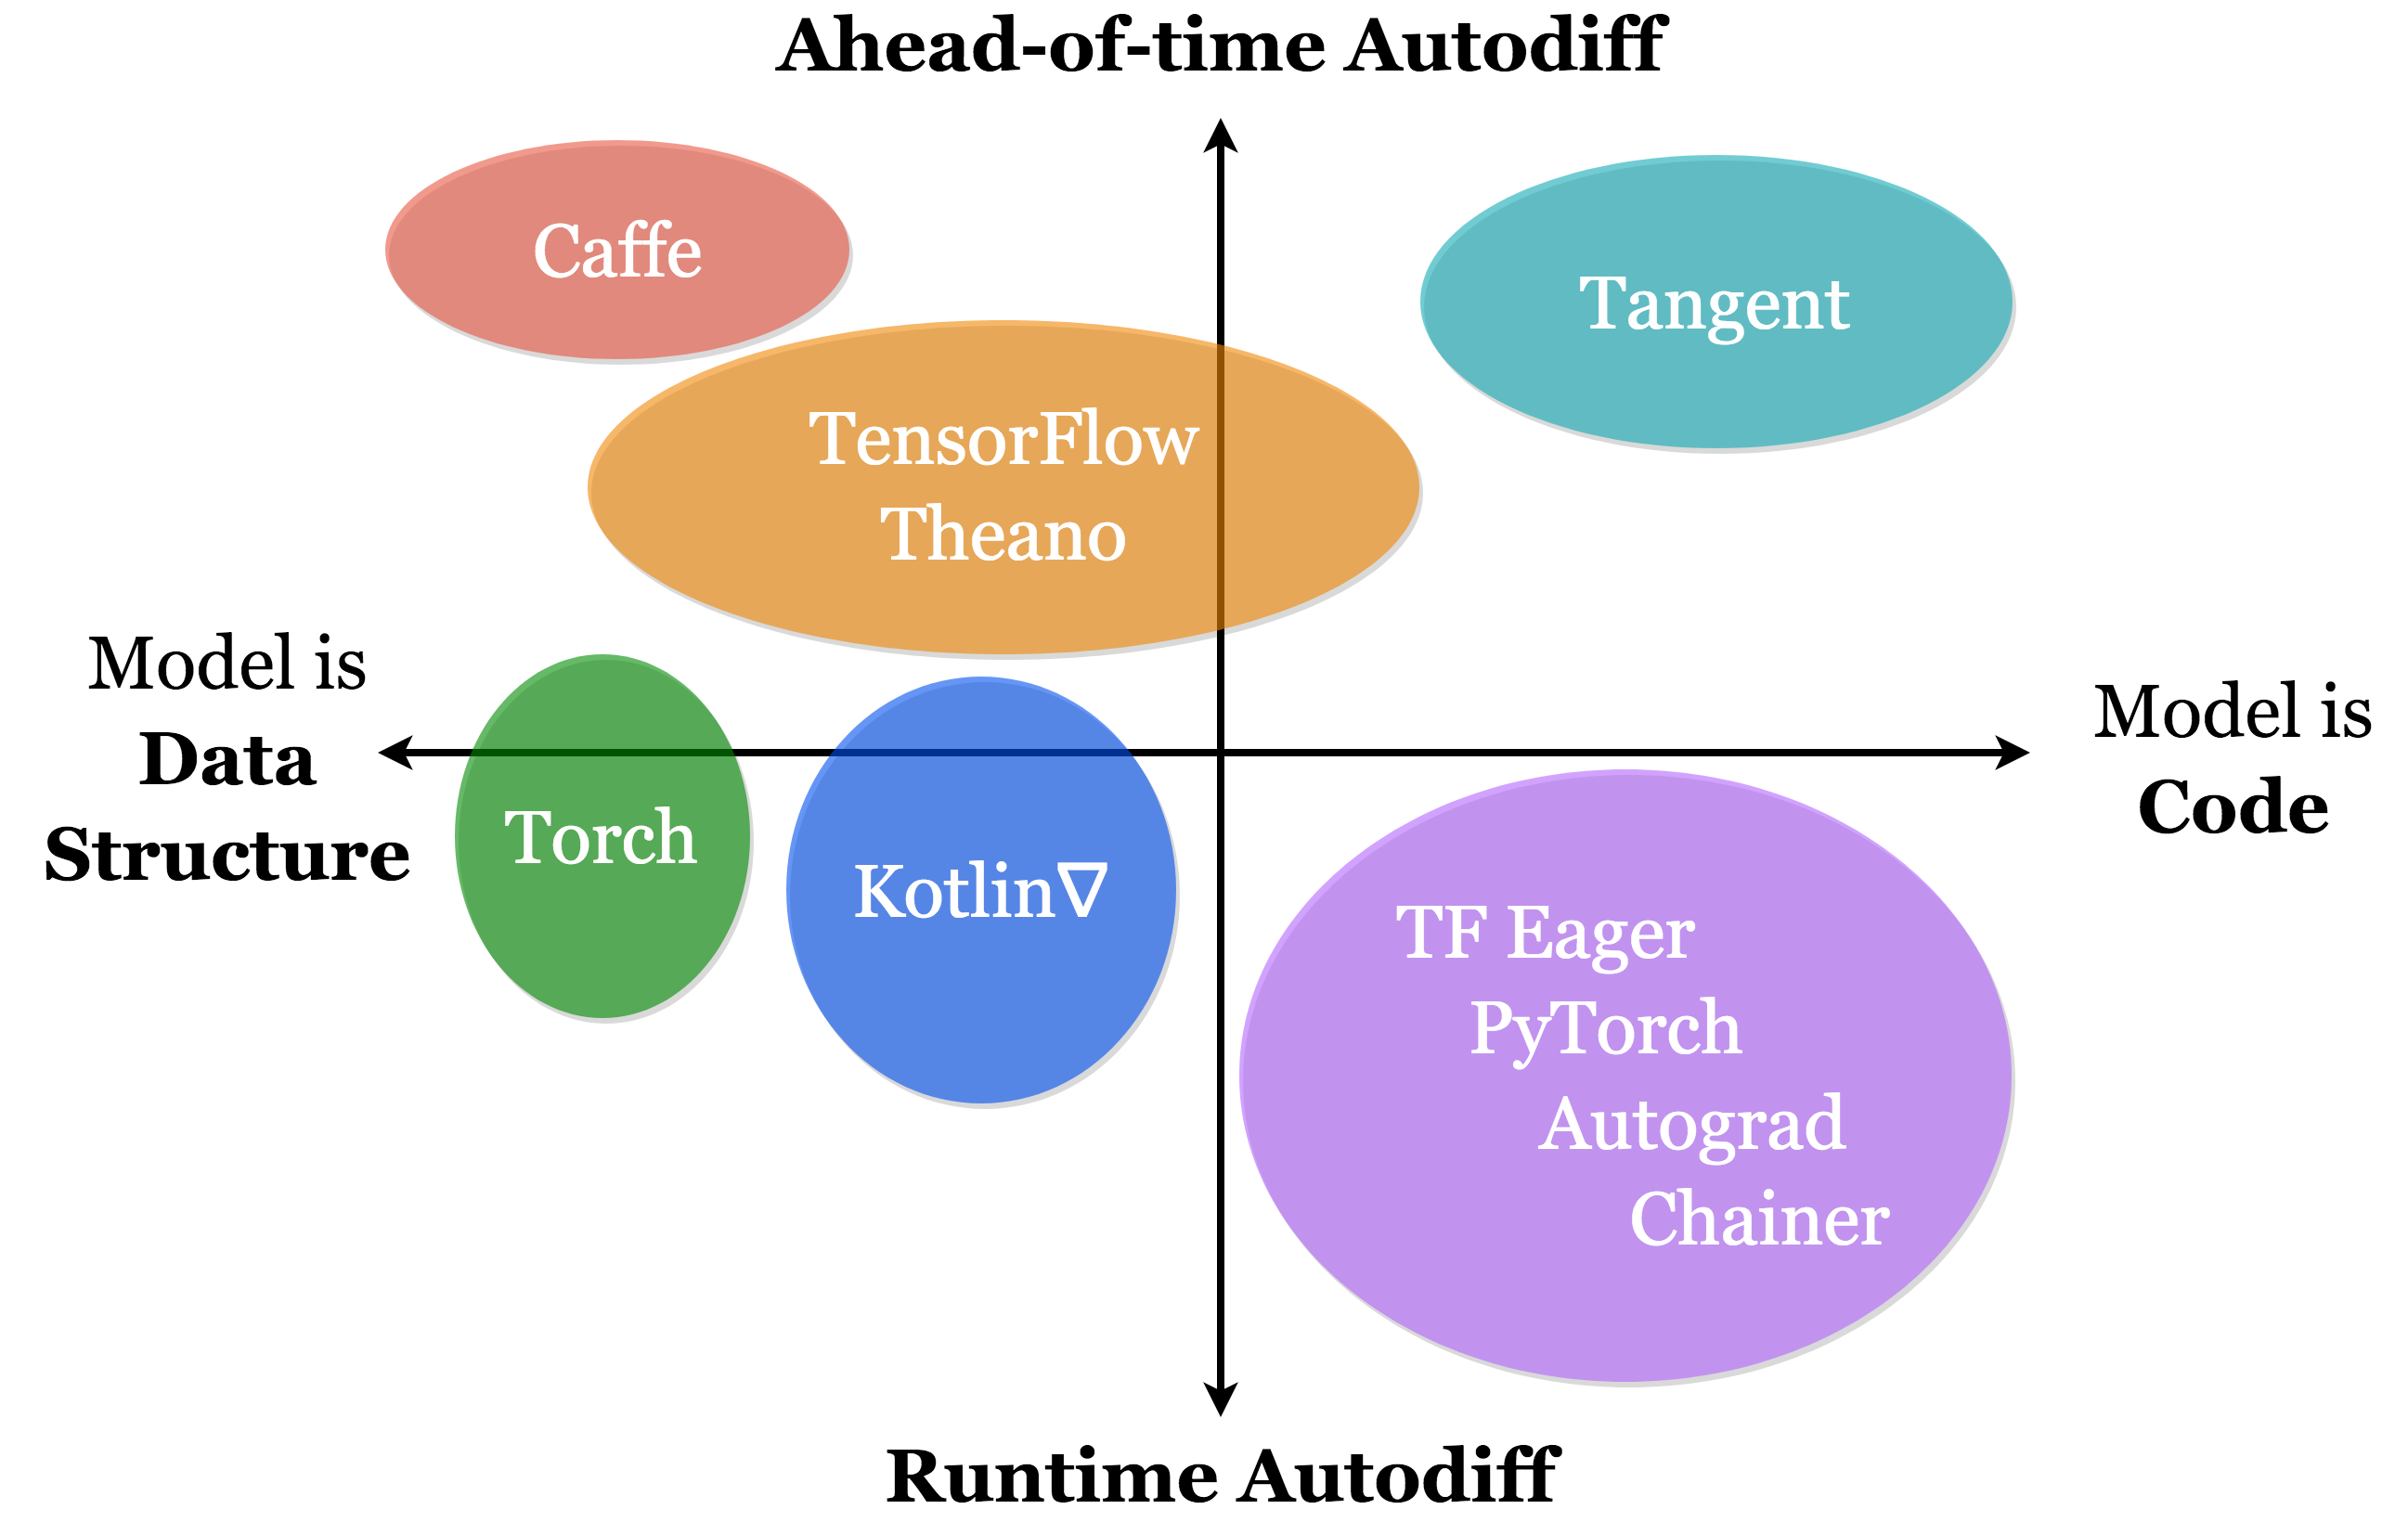
\includegraphics[width=0.70\textwidth]{../figures/kotlingrad_diagram.png}
\caption{Avec l'adaptation de~\citet{van2018tangent}. Les modèles Kotlin$\nabla$ sont des structures de données, construites par une DSL intégrée, ardemment optimisées et évaluées paresseusement.}
\label{fig:kotlingrad_digram}
\end{figure}

Les modèles Kotlin$\nabla$ sont des langages intégrés spécifiques à un domaine (eDSL). Ces langages peuvent apparaître et se comporter différemment du langage hôte, mais ne sont en réalité que des fonctions soigneusement déguisées pour construire un arbre syntaxique abstrait (AST). Souvent, ces AST représentent de simples machines à états, mais sont également utilisés pour intégrer un langage de programmation. Les exemples les plus courants sont \href{https://docs.microsoft.com/en-us/dotnet/framework/data/adonet/sql/linq/}{SQL/LINQ}~\citep{meijer2006linq}, \href{http://stanford-ppl.github.io/Delite/optiml/}{OptiML}~\citep{sujeeth2011optiml} et autres interfaces fluides~\citep{fowler05fluent}. Dans un langage hôte suffisamment expressif, on peut implémenter n'importe quel langage comme une bibliothèque, sans avoir besoin d'écrire un lexique, un analyseur, un compilateur ou un interpréteur. Et avec un typage approprié, les utilisateurs recevront des compléments de code et des analyses statiques de leurs outils de développement préférés. Les langages fonctionnels sont souvent des langages hôtes appropriés~\citep{elliott2003compiling,rompf2010lightweight}, peut-être en raison de la notion de code en tant que données.

\section{Usage}

Kotlin$\nabla$ permet aux utilisateurs de mettre en œuvre des programmes différentiables en composant des expressions. Considérons le programme Kotlin$\nabla$ suivant avec deux entrées et une sortie:
%
\begin{figure}[H] \label{fig:basic_kotlingrad}
\begin{unbreakablekotlin}
with(DoublePrecision) { // Utilise des chiffres en double précision
  val x par Var() // Déclarer des variables immuables (ces variables
  val y par Var() // sont seulement utilisées pour la différentiation)
  val z = sin(10 * (x * x + pow(y, 2))) / 10 // évaluation paresseuse
  val dz_dx = d(z) / d(x) // Notation Leibniz(*@~\citep{christianson2012leibniz}@*)
  val d2z_dxdy = d(dz_dx) / d(y) // Mélange de partiels d'ordre supérieur
  val d3z_d2xdy = grad(d2z_dxdy)[x] // Équivalent à d(f)/d(x)
  plot3D(d3z_d2xdy, -1.0, 1.0) // Tracé en espace 3 (-1 < x, y, z < 1)
}
\end{unbreakablekotlin}
%    \centering $z = \sin{\big(10(x*x + y^2)\big)} / 10$, \texttt{plot}$\Big\left(\frac{\partial^{3z}}{\partial{x^2}\partial{y}}\Big\right)$ \\
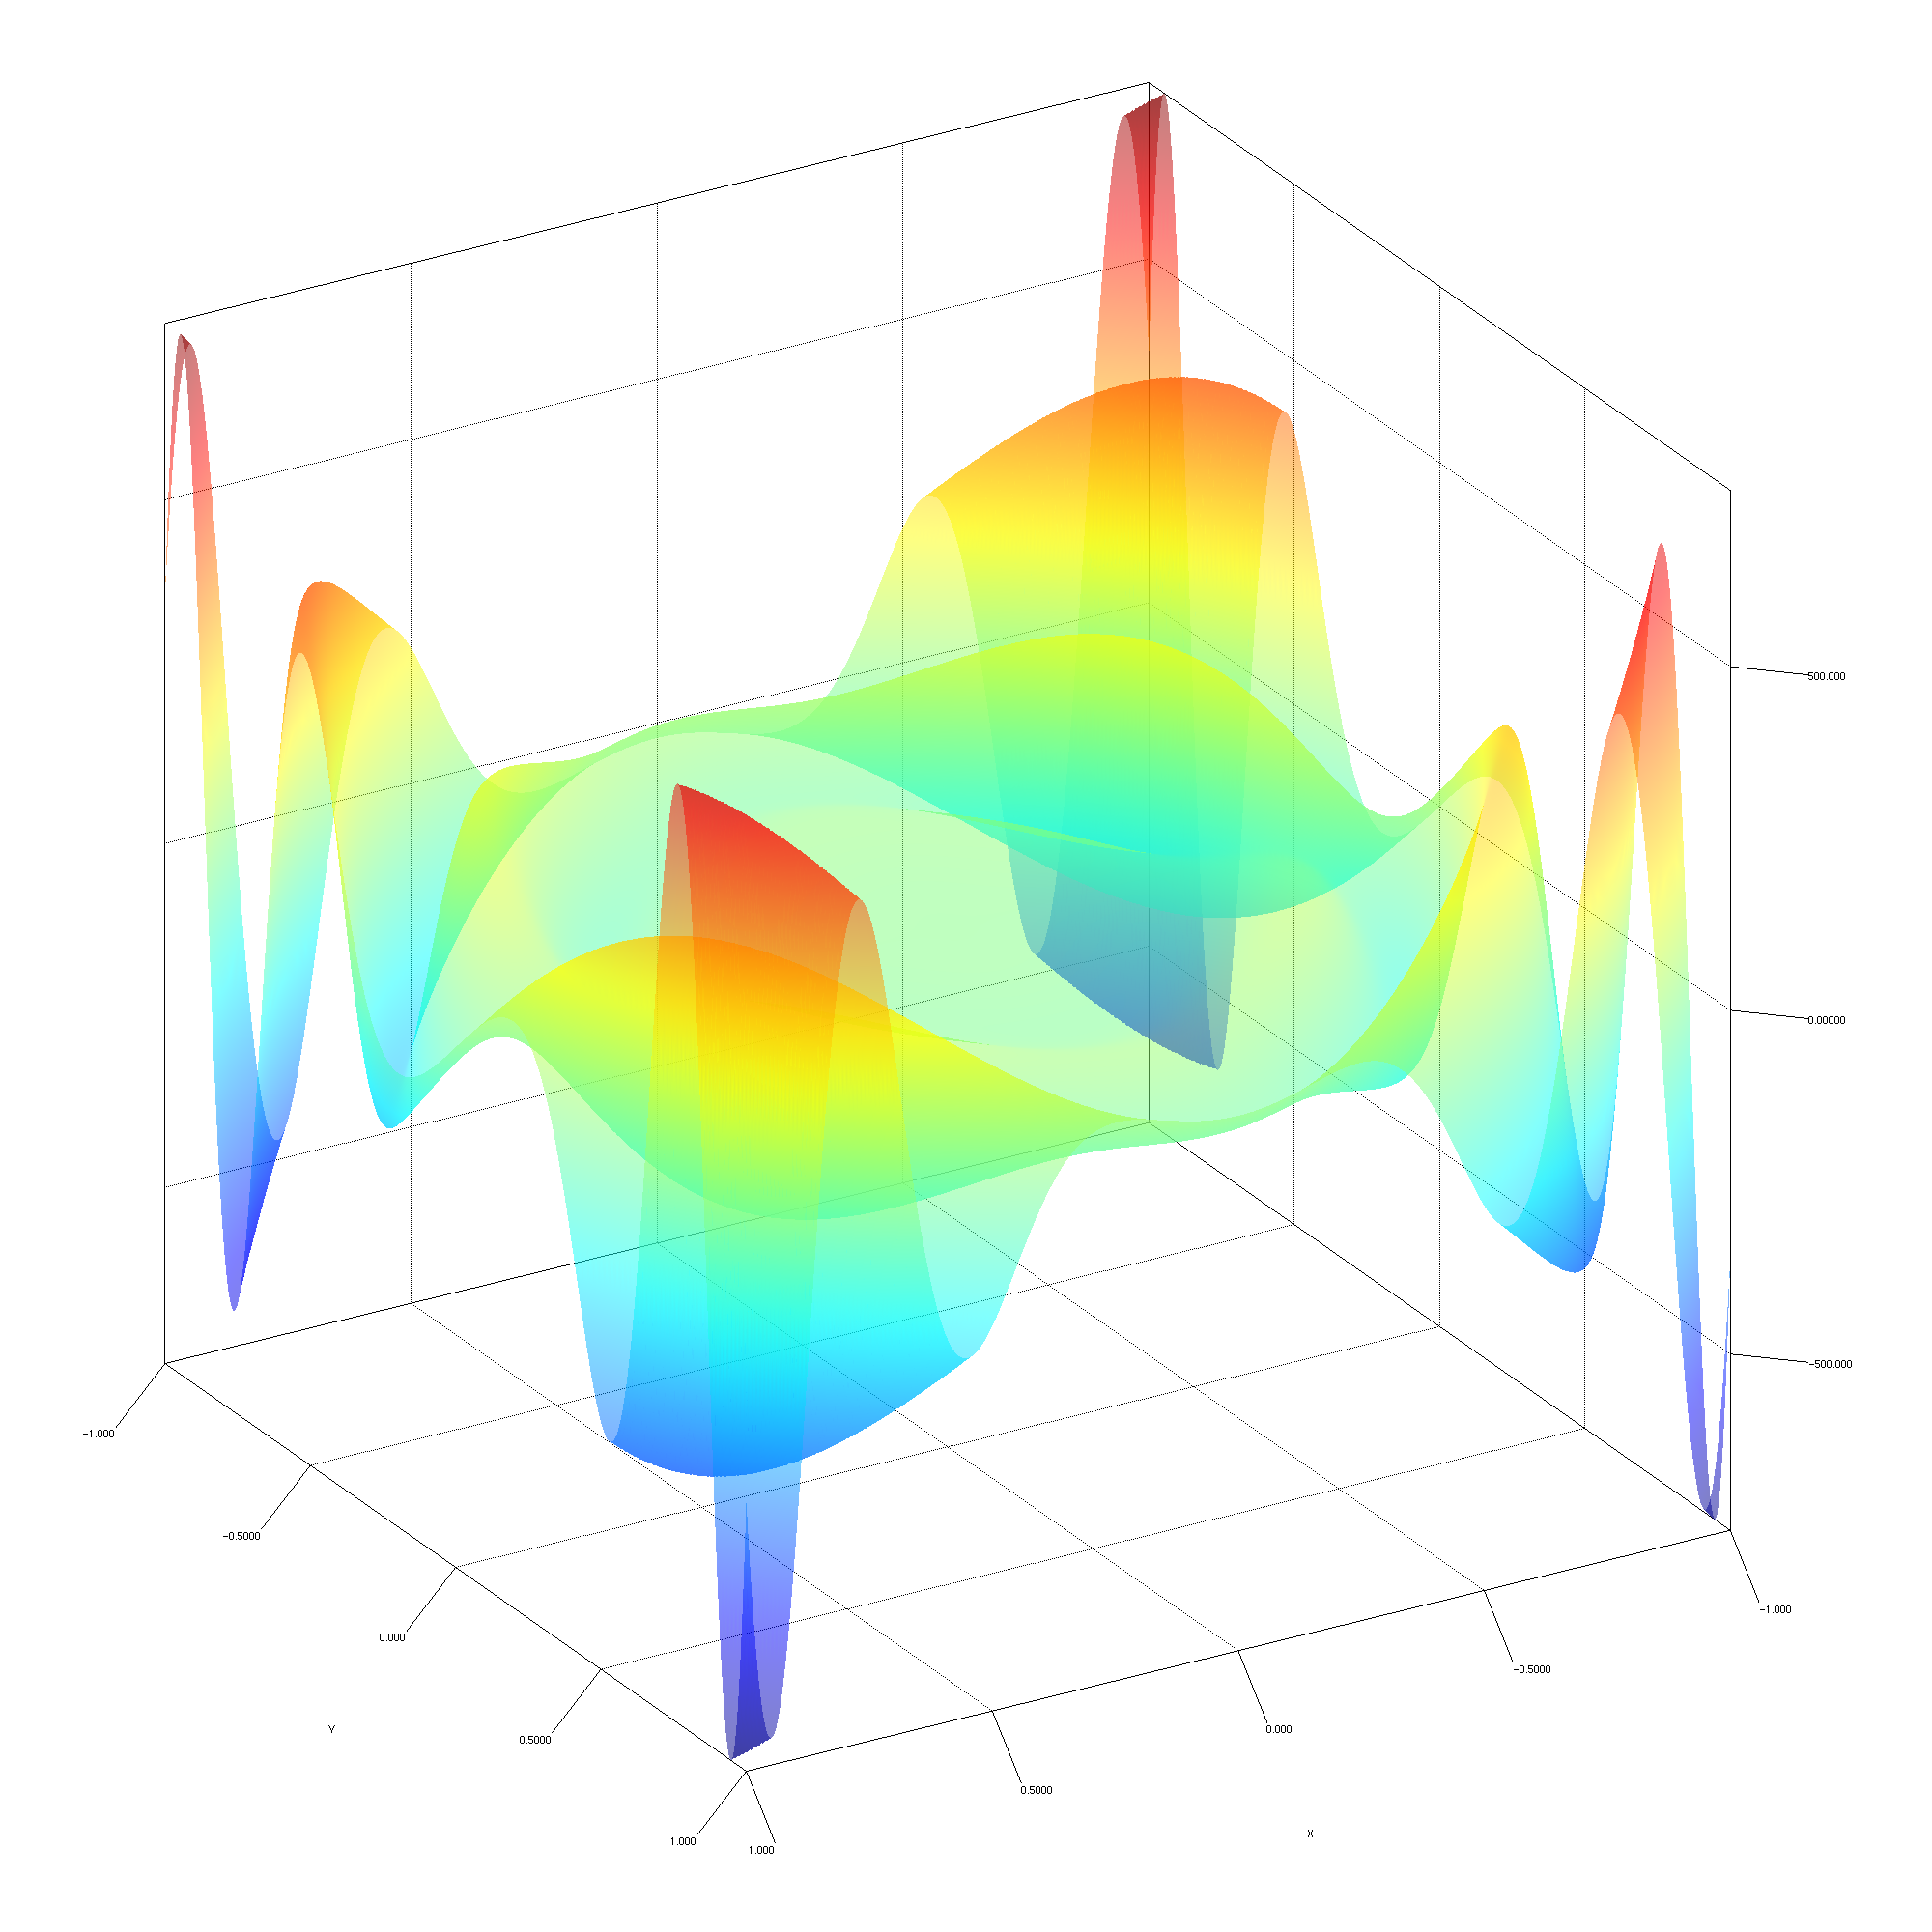
\includegraphics[scale=0.43]{../figures/plot_result.png}
\end{figure}
%
Ci-dessus, nous définissons une fonction à deux variables et prenons une série de dérivées partielles par rapport à chaque variable. Les expressions sont évaluées paresseusement dans un contexte numérique, qui peut être importé par fichier ou lexicalement pour un contrôle plus fin du comportement d'exécution. La fonction est évaluée numériquement sur l'intervalle $(-1, 1)$ dans chaque dimension et rendue dans l'espace 3. Pour une grammaire complète, veuillez vous référer à~\autoref{sec:kg_grammar}.
Nous pouvons également tracer des collecteurs à dimensions plus élevées (par exemple, la surface de perte d'un réseau neuronal), projetés en quatre dimensions et rendus en trois, où un axe est représenté par le temps.
%
\begin{figure}
%\begin{unbreakablekotlin}
%val z = sin(10 * (x * x + pow(y, 2))) / 10 // Does not perform calculation
%\end{unbreakablekotlin}
    \begin{unbreakablekotlin}
        val t = (1 + x * 2 + z / y).d(y).d(x) + z / y * 3 - 4 * (y pow y).d(y)
    \end{unbreakablekotlin}
\end{figure}
\vspace{-40pt}
\begin{figure}
    \centering
%\begin{tikzpicture}[grow=left]
%    \tikzset{level distance=60pt}
%    \Tree [.$\div$ [.\inline{sin} [.$\times$ \inline{10} [.$+$ [.$\times$ \inline{\textbf{x}} \inline{\textbf{x}} ] [.\inline{pow} \inline{\textbf{y}} \inline{2} ] ] ] ] \inline{10} ]
%\end{tikzpictre}
%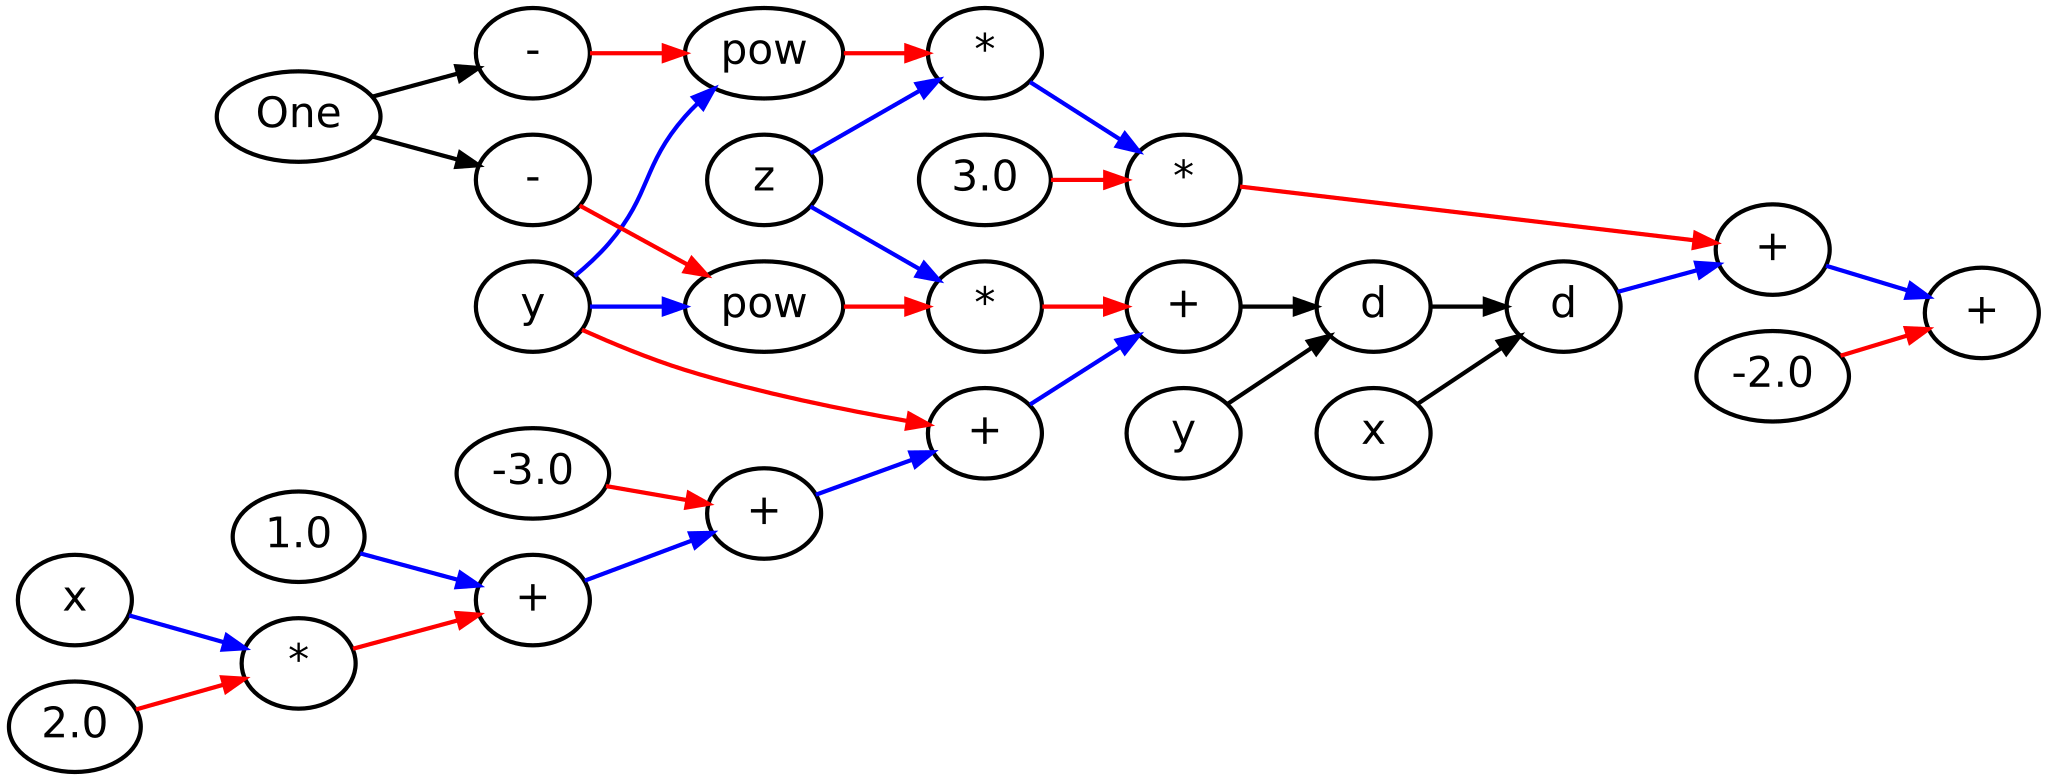
\includegraphics[scale=0.60]{../figures/dataflow.png}
    \digraph[scale=0.5]{dfg} { graph ["rankdir"="LR","bgcolor"="transparent"]; "209813603" ["color"="black","fontcolor"="black","fontname"="Helvetica","fontsize"="20","style"="setlinewidth(2)","label"="+"]; "659748578" ["color"="black","fontcolor"="black","fontname"="Helvetica","fontsize"="20","style"="setlinewidth(2)","label"="+"]; "483422889" ["color"="black","fontcolor"="black","fontname"="Helvetica","fontsize"="20","style"="setlinewidth(2)","label"="d"]; "1277181601" ["color"="black","fontcolor"="black","fontname"="Helvetica","fontsize"="20","style"="setlinewidth(2)","label"="d"]; "488970385" ["color"="black","fontcolor"="black","fontname"="Helvetica","fontsize"="20","style"="setlinewidth(2)","label"="+"]; "93122545" ["color"="black","fontcolor"="black","fontname"="Helvetica","fontsize"="20","style"="setlinewidth(2)","label"="+"]; "1239731077" ["color"="black","fontcolor"="black","fontname"="Helvetica","fontsize"="20","style"="setlinewidth(2)","label"="1.0"]; "249515771" ["color"="black","fontcolor"="black","fontname"="Helvetica","fontsize"="20","style"="setlinewidth(2)","label"="*"]; "x" ["color"="black","fontcolor"="black","fontname"="Helvetica","fontsize"="20","style"="setlinewidth(2)"]; "1627960023" ["color"="black","fontcolor"="black","fontname"="Helvetica","fontsize"="20","style"="setlinewidth(2)","label"="2.0"]; "1811044090" ["color"="black","fontcolor"="black","fontname"="Helvetica","fontsize"="20","style"="setlinewidth(2)","label"="*"]; "z" ["color"="black","fontcolor"="black","fontname"="Helvetica","fontsize"="20","style"="setlinewidth(2)"]; "940060004" ["color"="black","fontcolor"="black","fontname"="Helvetica","fontsize"="20","style"="setlinewidth(2)","label"="*"]; "1945604815" ["color"="black","fontcolor"="black","fontname"="Helvetica","fontsize"="20","style"="setlinewidth(2)","label"="*"]; "328638398" ["color"="black","fontcolor"="black","fontname"="Helvetica","fontsize"="20","style"="setlinewidth(2)","label"="pow"]; "y" ["color"="black","fontcolor"="black","fontname"="Helvetica","fontsize"="20","style"="setlinewidth(2)"]; "1121172875" ["color"="black","fontcolor"="black","fontname"="Helvetica","fontsize"="20","style"="setlinewidth(2)","label"="pow"]; "1644443712" ["color"="black","fontcolor"="black","fontname"="Helvetica","fontsize"="20","style"="setlinewidth(2)","label"="pow"]; "745160567" ["color"="black","fontcolor"="black","fontname"="Helvetica","fontsize"="20","style"="setlinewidth(2)","label"="d"]; "391447681" ["color"="black","fontcolor"="black","fontname"="Helvetica","fontsize"="20","style"="setlinewidth(2)","label"="*"]; "1308927845" ["color"="black","fontcolor"="black","fontname"="Helvetica","fontsize"="20","style"="setlinewidth(2)","label"="-"]; "440434003" ["color"="black","fontcolor"="black","fontname"="Helvetica","fontsize"="20","style"="setlinewidth(2)","label"="-"]; "1" ["color"="black","fontcolor"="black","fontname"="Helvetica","fontsize"="20","style"="setlinewidth(2)","label"="One"]; "1595953398" ["color"="black","fontcolor"="black","fontname"="Helvetica","fontsize"="20","style"="setlinewidth(2)","label"="-"]; "1277181601{color=black, fontcolor=black, fontname=Helvetica, fontsize=20, style=setlinewidth(2)}->" ["color"="black","fontcolor"="black","fontname"="Helvetica","fontsize"="20","style"="setlinewidth(2)","label"="y"]; "483422889{color=black, fontcolor=black, fontname=Helvetica, fontsize=20, style=setlinewidth(2)}->" ["color"="black","fontcolor"="black","fontname"="Helvetica","fontsize"="20","style"="setlinewidth(2)","label"="x"]; "1684106402" ["color"="black","fontcolor"="black","fontname"="Helvetica","fontsize"="20","style"="setlinewidth(2)","label"="3.0"]; "403424356" ["color"="black","fontcolor"="black","fontname"="Helvetica","fontsize"="20","style"="setlinewidth(2)","label"="4.0"]; "745160567{color=black, fontcolor=black, fontname=Helvetica, fontsize=20, style=setlinewidth(2)}->" ["color"="black","fontcolor"="black","fontname"="Helvetica","fontsize"="20","style"="setlinewidth(2)","label"="y"]; "659748578" -> "209813603" ["color"="blue","arrowhead"="normal","style"="setlinewidth(2)"]; "483422889" -> "659748578" ["color"="blue","arrowhead"="normal","style"="setlinewidth(2)"]; "1277181601" -> "483422889" ["color"="black","arrowhead"="normal","style"="setlinewidth(2)"]; "488970385" -> "1277181601" ["color"="black","arrowhead"="normal","style"="setlinewidth(2)"]; "93122545" -> "488970385" ["color"="blue","arrowhead"="normal","style"="setlinewidth(2)"]; "1239731077" -> "93122545" ["color"="blue","arrowhead"="normal","style"="setlinewidth(2)"]; "249515771" -> "93122545" ["color"="red","arrowhead"="normal","style"="setlinewidth(2)"]; "x" -> "249515771" ["color"="blue","arrowhead"="normal","style"="setlinewidth(2)"]; "1627960023" -> "249515771" ["color"="red","arrowhead"="normal","style"="setlinewidth(2)"]; "1811044090" -> "488970385" ["color"="red","arrowhead"="normal","style"="setlinewidth(2)"]; "z" -> "1811044090" ["color"="blue","arrowhead"="normal","style"="setlinewidth(2)"]; "z" -> "940060004" ["color"="blue","arrowhead"="normal","style"="setlinewidth(2)"]; "940060004" -> "1945604815" ["color"="blue","arrowhead"="normal","style"="setlinewidth(2)"]; "1945604815" -> "659748578" ["color"="red","arrowhead"="normal","style"="setlinewidth(2)"]; "328638398" -> "1811044090" ["color"="red","arrowhead"="normal","style"="setlinewidth(2)"]; "y" -> "328638398" ["color"="blue","arrowhead"="normal","style"="setlinewidth(2)"]; "y" -> "1121172875" ["color"="blue","arrowhead"="normal","style"="setlinewidth(2)"]; "y" -> "1644443712" ["color"="blue","arrowhead"="normal","style"="setlinewidth(2)"]; "y" -> "1644443712" ["color"="red","arrowhead"="normal","style"="setlinewidth(2)"]; "1121172875" -> "940060004" ["color"="red","arrowhead"="normal","style"="setlinewidth(2)"]; "1644443712" -> "745160567" ["color"="black","arrowhead"="normal","style"="setlinewidth(2)"]; "745160567" -> "391447681" ["color"="red","arrowhead"="normal","style"="setlinewidth(2)"]; "391447681" -> "1308927845" ["color"="black","arrowhead"="normal","style"="setlinewidth(2)"]; "1308927845" -> "209813603" ["color"="red","arrowhead"="normal","style"="setlinewidth(2)"]; "440434003" -> "328638398" ["color"="red","arrowhead"="normal","style"="setlinewidth(2)"]; "1" -> "440434003" ["color"="black","arrowhead"="normal","style"="setlinewidth(2)"]; "1" -> "1595953398" ["color"="black","arrowhead"="normal","style"="setlinewidth(2)"]; "1595953398" -> "1121172875" ["color"="red","arrowhead"="normal","style"="setlinewidth(2)"]; "1277181601{color=black, fontcolor=black, fontname=Helvetica, fontsize=20, style=setlinewidth(2)}->" -> "1277181601" ["color"="black","arrowhead"="normal","style"="setlinewidth(2)"]; "483422889{color=black, fontcolor=black, fontname=Helvetica, fontsize=20, style=setlinewidth(2)}->" -> "483422889" ["color"="black","arrowhead"="normal","style"="setlinewidth(2)"]; "1684106402" -> "1945604815" ["color"="red","arrowhead"="normal","style"="setlinewidth(2)"]; "403424356" -> "391447681" ["color"="blue","arrowhead"="normal","style"="setlinewidth(2)"]; "745160567{color=black, fontcolor=black, fontname=Helvetica, fontsize=20, style=setlinewidth(2)}->" -> "745160567" ["color"="black","arrowhead"="normal","style"="setlinewidth(2)"]; }

    \caption{DFG implicite construit par l'expression originale, montrée ci-dessus.}
    \label{lst:edsl}
\end{figure}\\\\

\section{Systèmes de typage}\label{sec:type-systems}

Les premiers travaux sur l'analyse dimensionnelle sans risque de type se trouvent dans \citet{kennedy1994dimension, kennedy1996programming} qui utilise les types pour coder la dimensionnalité et empêcher l'apparition de bogues courants liés à la non-concordance des dimensions, et a été réalisé plus tard dans le langage F\#~\citep{kennedy2010types}. \citet{jay1996shape}, \citet{rittri1995dimension}, et \citet{zenger1997indexed} explorent l'application des types de dimension pour l'algèbre linéaire. Plus récemment, \citet{kiselyov2005number, kiselyov2010fun} et \citet{griffioen2015type}, montrent comment manipuler des tableaux de manière plus complexe. Avec le regain d'intérêt pour l'algèbre des tenseurs et la programmation des tableaux, \citet{chen2017typesafe} et \citet{rink2018modeling} montrent comment coder la sécurité des formes pour l'algèbre des tenseurs dans divers systèmes de types.

Le problème que nous essayons de résoudre peut être résumé comme suit. Étant donné deux valeurs \inline{x} et \inline{y}, et l'opérateur \inline{\$}, comment déterminer si l'expression \inline{z = x \$ y} est valide, et si oui, quel est le type de résultat de \inline{z}? Pour la multiplication matricielle, lorsque \inline{x} $\in \mathbb{R}^{m \times n}$ et \inline{y} $\in \mathbb{R}^{n \times p}$, l'expression est bien tapée et nous pouvons déduire \inline{z} $\in \mathbb{R}^{m \times p}$. Plus généralement, nous voudrions déduire le type de \inline{z} pour un opérateur quelconque \inline{@} $ : (\mathbb{R}^\mathbf{a}, \mathbb{R}^\mathbf{b}) \rightarrow \mathbb{R}^\mathbf{c}$ où $\mathbf{a} \in \mathbb{N}^q, \mathbf{b} \in \mathbb{N}^r, \mathbf{c} \in \mathbb{N}^s$ et $q, r, s \in \mathbb{N}$. Pour de nombreuses opérations d'algèbre linéaire telles que la multiplication de matrices, $\mathcal{S}(\mathbf a, \mathbf b) \stackrel{?}{=} \mathbf c$ est calculable en $\mathcal{O}(1)$ -- on peut simplement vérifier l'équivalence des dimensions intérieures ($\mathbf{a}_2 \stackrel{?}{=} \mathbf{b}_1$).

La vérification de forme des opérateurs de tableaux multidimensionnels n'est pas toujours décidable. Pour les fonctions de forme arbitraires $\mathcal{S}(\mathbf{a}, \mathbf{b})$, la vérification $\mathcal{S}(\mathbf{a}, \mathbf{b}) \stackrel{?}{=} \mathbf{c}$ nécessite une machine de Turing. Si $\mathcal{S}$ utilise l'opérateur de multiplication, comme dans le cas de l'arithmétique convolutionnelle~\citep{dumoulin2016guide}, l'inférence de forme devient équivalente à l'arithmétique Peano, qui est indécidable~\citep{godel1931formal}. L'addition, la soustraction, l'indexation et la comparaison d'entiers sont toutes décidables en arithmétique de Presburger~\citep{suzuki1980verification, bradley2006decidable, charlier2011enumeration}. La vérification de l'égalité est trivialement décidable, et peut être mise en œuvre dans la plupart des systèmes de type statique.

L'évaluation d'un $\mathcal{S}$ arbitraire qui utilise la multiplication ou la division (par exemple, arithmétique convolutionnelle) nécessite un langage typé de manière dépendante ~\citep{xi1998eliminating, pineyro2019structure}, mais la vérification de l'égalité de forme (par exemple la vérification de forme des opérations arithmétiques ordinaires) est possible Java et ses cousins.\hspace{-.08em}\footnote{Le système de types de Java est connu pour être complet à Turing~\citep{grigore2017java}. Ainsi, l'émulation de types dépendants en Java est théoriquement possible, mais probablement insoluble en raison des limitations pratiques notées par Grigore.} De plus, nous pensons que la vérification de forme de l'arithmétique matricielle ordinaire est décidable dans tout système de type librement basé sur le système F${}_{<:}$~\citep{cardelli1991extension}. Nous proposons un système de types pour renforcer la sécurité des formes qui peut être mis en œuvre dans n'importe quel langage avec sous-typage et génériques, comme \href{https://docs.oracle.com/javase/tutorial/java/generics/index.html}{Java}~\citep{naftalin2007java}, \href{https://kotlinlang.org/docs/reference/generics.html}{Kotlin}~\citep{tate2013mixed}, \href{https://www.typescriptlang.org/docs/handbook/advanced-types.html}{TypeScript}~\citep{bierman2014understanding} ou \href{https://doc.rust-lang.org/1.7.0/book/generics.html}{Rust}~\citep{crozet2019nalgebra}.

{\tiny
    \begin{table}
        \begin{tabular}{|c||c|c|c|l|}\hline
            Math                                     &  Infix                                                                           & Prefix                                                                                    & Postfix                                                                                      & Operator Type Signature                                                                                                                                                                                      \\ \hline
            $A(B)$                                                         & \tinline{a(b)}                                                                   &                                                                                           &                                                                                              & $ (\texttt{a}:  \mathbb{R}^{\tau}\rightarrow\mathbb{R}^{\pi}, \texttt{b}: \mathbb{R}^{\lambda} \rightarrow \mathbb{R}^{\tau}) \rightarrow (\mathbb{R}^{\lambda}\rightarrow \mathbb{R}^{\pi})               $ \\ \hline
            $A\pm B$                                                       & \begin{tabular}{@{}c@{}}\tinline{a + b}\\\tinline{a - b}\end{tabular}            & \begin{tabular}{@{}c@{}}\tinline{plus(a, b)}\\\tinline{minus(a, b)}\end{tabular}          &                                                                                              & $ (\texttt{a}:  \mathbb{R}^{\tau}\rightarrow\mathbb{R}^{\pi}, \texttt{b}: \mathbb{R}^{\lambda} \rightarrow \mathbb{R}^{\pi}) \rightarrow (\mathbb{R}^{?}\rightarrow \mathbb{R}^{\pi})                      $ \\ \hline
            $A   B$                                                        & \begin{tabular}{@{}c@{}}\tinline{a * b}\\\tinline{a.times(b)}\end{tabular}       & \tinline{times(a, b)}                                                                     &                                                                                              & $ (\texttt{a}: \mathbb{R}^{\tau}\rightarrow\mathbb{R}^{m \times n}, \texttt{b}: \mathbb{R}^{\lambda}\rightarrow\mathbb{R}^{n \times p})    \rightarrow (\mathbb{R}^{?}\rightarrow\mathbb{R}^{m \times p})  $ \\ \hline
            \begin{tabular}{@{}c@{}}$\frac{A}{B}$\\$AB^{-1}$\end{tabular}  & \begin{tabular}{@{}c@{}}\tinline{a / b}\\\tinline{a.div(b)}\end{tabular}         & \tinline{div(a, b)}                                                                       &                                                                                              & $ (\texttt{a}: \mathbb{R}^{\tau}\rightarrow\mathbb{R}^{m \times n}, \texttt{b}: \mathbb{R}^{\lambda}\rightarrow\mathbb{R}^{p \times n}) \rightarrow (\mathbb{R}^{?}\rightarrow\mathbb{R}^{m \times p})     $ \\ \hline
            $\pm A$                                                        &                                                                                  & \begin{tabular}{@{}c@{}}\tinline{-a}\\\tinline{+a}\end{tabular}                           & \begin{tabular}{@{}c@{}}\tinline{a.unaryMinus()}\\\tinline{a.unaryPlus()}\end{tabular}       & $                   (\texttt{a}: \mathbb{R}^{\tau}\rightarrow\mathbb{R}^{\pi}) \rightarrow (\mathbb{R}^{\tau}\rightarrow\mathbb{R}^{\pi})                                                                  $ \\ \hline
%\begin{tabular}{@{}c@{}}sin(a)\\cos(a)\\tan(a)\end{tabular}               &                                                                                  & \begin{tabular}{@{}c@{}}\tinline{sin(a)}\\\tinline{cos(a)}\\\tinline{tan(a)}\end{tabular} & \begin{tabular}{@{}c@{}}\tinline{a.sin()}\\\tinline{a.cos()}\\\tinline{a.tan()}\end{tabular} & $                                            (\texttt{a}: \mathbb{R}\rightarrow\mathbb{R}) \rightarrow (\mathbb{R}\rightarrow\mathbb{R})                                                                   $ \\ \hline
            $\ln(A)$                                                       &                                                                                  & \begin{tabular}{@{}c@{}}\tinline{ln(a)}\\\tinline{log(a)}\end{tabular}                    & \begin{tabular}{@{}c@{}}\tinline{a.ln()}\\\tinline{a.log()}\end{tabular}                     & $                  (\texttt{a}: \mathbb{R}^{\tau}\rightarrow\mathbb{R}^{m \times m}) \rightarrow (\mathbb{R}^{\tau}\rightarrow\mathbb{R}^{m \times m})                                                     $ \\ \hline
            $\log_b A$                                                     & \tinline{a.log(b)}                                                               & \tinline{log(a, b)}                                                                       &                                                                                              & $       (\texttt{a}: \mathbb{R}^{\tau}\rightarrow\mathbb{R}^{m \times m}, \texttt{b}: \mathbb{R}^{\lambda}\rightarrow\mathbb{R}^{m \times m}) \rightarrow (\mathbb{R}^{?}\rightarrow\mathbb{R})            $ \\ \hline
            $A^{b}$                                                        & \tinline{a.pow(b)}                                                               & \tinline{pow(a, b)}                                                                       &                                                                                              & $       (\texttt{a}: \mathbb{R}^{\tau}\rightarrow\mathbb{R}^{m \times m}, \texttt{b}: \mathbb{R}^{\lambda}\rightarrow\mathbb{R}) \rightarrow (\mathbb{R}^{?}\rightarrow\mathbb{R}^{m \times m})            $ \\ \hline
            \begin{tabular}{@{}c@{}}$\sqrt{a}$\\$\sqrt[3]{a}$\end{tabular} & \begin{tabular}{@{}c@{}}\tinline{a.pow(1.0/2)}\\\tinline{a.root(3)}\end{tabular} & \begin{tabular}{@{}c@{}}\tinline{a.pow(1.0/2)}\\\tinline{a.root(3)}\end{tabular}          & \begin{tabular}{@{}c@{}}\tinline{a.sqrt()}\\\tinline{a.cbrt()}\end{tabular}                  & $                        (\texttt{a}: \mathbb{R}^{\tau}\rightarrow\mathbb{R}^{m \times m}) \rightarrow (\mathbb{R}\rightarrow\mathbb{R}^{m \times m})                                                      $ \\ \hline
            \begin{tabular}{@{}c@{}}$\frac{da}{db}$\\$a'(b)$\end{tabular}  & \tinline{a.d(b)}                                                                 & \tinline{grad(a)[b]}                                                                      & \tinline{d(a) / d(b)}                                                                        & $         (\texttt{a}: \mathbb{R}^{\tau}\rightarrow\mathbb{R}^{\pi}, \texttt{b}: \mathbb{R}^{\lambda}\rightarrow\mathbb{R}^{\omega}) \rightarrow (\mathbb{R}^{?}\rightarrow\mathbb{R}^{\pi \times \omega}) $ \\ \hline
        \end{tabular}
        \caption{\label{tab:shape_system}Kotlin$\nabla$ spécifie la forme de sortie pour les expressions tensorielles.}
    \end{table}
}
%$\dagger$ \inline{a} et \inline{b} sont des fonctions d'ordre supérieur. Il peut s'agir de constantes (par exemple 0, 1.0), de variables (par exemple \inline{Var("x")}) ou d'expressions (par exemple \inline{x + 1}, \inline{2 * x + y}).

{\small
\begin{table}[]
    \begin{tabular}{|c|c|c|c|}\hline
        Forme & $\mathbb{R}^{?}\rightarrow\mathbb{R}$ & $\mathbb{R}^{?}\rightarrow\mathbb{R}^{m}$ & $\mathbb{R}^{?}\rightarrow\mathbb{R}^{j \times k}$ \\\hline
    $\mathbb{R}^{?}\rightarrow\mathbb{R}$ & $\mathbb{R}^{?}\rightarrow\mathbb{R}$ & $\mathbb{R}^{?}\rightarrow\mathbb{R}^{m}$ & $\mathbb{R}^{?}\rightarrow\mathbb{R}^{j \times k}$ \\\hline
    $\mathbb{R}^{?}\rightarrow\mathbb{R}^{n}$ & $\mathbb{R}^{?}\rightarrow\mathbb{R}^{n}$  & $\mathbb{R}^{?}\rightarrow\mathbb{R}^{m \times n}$  &  \\\hline
    $\mathbb{R}^{?}\rightarrow\mathbb{R}^{h \times i}$ & $\mathbb{R}^{?}\rightarrow\mathbb{R}^{h \times i}$  &  &\\\hline
    \end{tabular}
    \caption{\label{tab:ho_deriv}La forme d'une dérivée du tenseur dépend de la forme de la fonction en cours de différentiation et de la forme de la variable par rapport à laquelle nous nous différencions.}
\end{table}
}

\section{Sécurité de la forme}\label{sec:shape-safety}

\noindent Il existe trois grandes stratégies pour traiter les erreurs de forme dans la programmation des tableaux:
%
\begin{enumerate}
    \item Cacher l'erreur en remodelant implicitement ou \href{https://docs.scipy.org/doc/numpy-1.15.0/user/basics.broadcasting.html}{broadcasting arrays}.
    \item Annoncer l'erreur au moment de l'exécution, par exemple: ~\href{https://www.tensorflow.org/api_docs/python/tf/errors/InvalidArgumentError}{\inline{InvalidArgumentError}}.
    \item Ne pas autoriser la compilation de programmes pouvant entraîner une erreur de forme. \\
\end{enumerate}
%
La plupart des bibliothèques de programmation de tableaux telles que NumPy~\citep{van2011numpy} ou TensorFlow~\citep{abadi2016tensorflow} utilisent la première ou la deuxième stratégie. Dans Kotlin$\nabla$, nous adoptons la troisième, qui permet à un vérificateur de type incrémental, comme ceux que l'on trouve généralement dans les EDI modernes, de détecter instantanément quand une opération de matrice est invalide. Prenons l'exemple suivant:
%
\begin{kotlinlisting}
val vecA = Vec(1.0, 2.0)      // Type inféré : Vec<Int, D2>
val vecB = Vec(1.0, 2.0, 3.0) // Type inféré : Vec<Int, D3>
val vecC = vecB + vecB
val vecD = (*@\uwave{vecA + vecB}@*) // Erreur de compilation: Expected Vec<2>, found Vec<3>
\end{kotlinlisting}
%
Tenter de faire la somme de deux vecteurs dont les formes ne correspondent pas, c'est échouer à la compilation.
%
\begin{kotlinlisting}
val matA = Mat1x4(1.0, 2.0, 3.0, 4.0) // Type inféré: Mat<Double, D1, D4>
val matB = Mat4x1(1.0, 2.0, 3.0, 4.0) // Type inféré: Mat<Double, D4, D1>
val matC = matA * matB
val matD = (*@\uwave{matA *\ matC}@*) // Erreur de compilation: Expected <4, *>, found Mat<1, 1>
\end{kotlinlisting}
%
De même, la multiplication de deux matrices dont les dimensions intérieures ne correspondent pas ne permet pas de compiler.
%
\begin{kotlinlisting}
val matA = Mat2x4(1.0, 2.0, 3.0, 4.0,
                  5.0, 6.0, 7.0, 8.0)
val matB = Mat4x2(1.0, 2.0,
                  3.0, 4.0,
                  5.0, 6.0,
                  7.0, 8.0)
val matC: Mat<Double, D2, D2> = a * b // Les types sont facultatifs, mais encouragés
val matD = Mat2x1(1.0, 2.0)
val matE = matC * matD
val matF = Mat3x1(1.0, 2.0, 3.0)
val matG = (*@\uwave{matE *\ matF}@*) // Erreur de compilation: Expected Mat<1, *>, found Mat<3, 1>
\end{kotlinlisting}
%
Il est nécessaire de spécifier les types de paramètres dans une signature de méthode. Les types de retour explicites sont facultatifs mais sont encouragés pour des raisons de lisibilité. S'ils sont omis, le système de types peut souvent les déduire:
%
\begin{kotlinlisting}
fun someMatFun(m: Mat<Double, D3, D1>): Mat<Double, D3, D3> = ...
fun someMatFun(m: Mat<Double, D2, D2>) = ...
\end{kotlinlisting}
%
La sécurité des formes est actuellement prise en charge jusqu'aux tenseurs de rang 2, c'est-à-dire les matrices. Pour effectuer la vérification des dimensions dans notre système de types, nous énumérons d'abord une liste de types littéraux entiers comme une chaîne de sous-types, $C < : C - 1 < : C - 2 < : \dots < : 1 < : 0$, où $C$ est la plus grande dimension de longueur fixe que nous souhaitons représenter, qui peut être spécifiée par l'utilisateur avant la compilation. Cela garantit une complexité linéaire dans l'espace et le temps pour le contrôle des sous-types, avec une limite supérieure constante.
%
\begin{kotlinlisting}[caption={Type sécurisé pour les tenseurs de rang 1, $\forall C\leq2.$}]
interface Nat<T: D0> { val i: Int }
// Les valeurs Int ont été réifiées pour permettre de les comparer à l'exécution
sealed class D0(open val i: Int = 0) { companion object: D0(), Nat<D0> }
sealed class D1(override val i: Int = 1): D0(i) { companion object: D1(), Nat<D1> }
sealed class D2(override val i: Int = 2): D1(i) { companion object: D2(), Nat<D2> }
sealed class D3(override val i: Int = 3): D2(i) { companion object: D3(), Nat<D3> } //...
sealed class D99(override val i: Int = 99): D98(i) { companion object: D99(), Nat<D99> }
\end{kotlinlisting}
%
Ensuite, nous surchargeons l'opérateur d'appel pour émuler l'instanciation d'une collection littérale, en utilisant l'arité pour en déduire la dimensionnalité. Considérons le cas du rang 1 pour l'inférence de longueur sur des littéraux vectoriels:
%
\begin{kotlinlisting}
open class Vec<E, Len: D1> constructor(val contents: List<E>) {
    companion object {
        operator fun <T> invoke(t: T): Vec<T, D1> = Vec(listOf(t))
        operator fun <T> invoke(t0: T, t1: T): Vec<T, D2> = Vec(listOf(t0, t1))
        operator fun <T> invoke(t0: T, t1: T, t2: T): Vec<T, D3> = Vec(listOf(t0, t1, t2))
    }
}
\end{kotlinlisting}
%
Enfin, nous surchargeons les opérateurs arithmétiques en utilisant des contraintes de forme génériques. Comme nos entiers de niveau type sont une chaîne de sous-types, nous n'avons besoin de définir qu'un seul opérateur et pouvons compter sur la substitution de Liskov~\citep{liskov1987} pour préserver la sécurité des formes pour tous les sous-types.
%
\begin{kotlinlisting}
// <C: D1> acceptera 1 <= C <= 99 via la substitution Liskov
operator fun <E, C: D1, V: Vec<X, C>> V.plus(v: V): V = TODO()
\end{kotlinlisting}
%
L'opérateur \inline{+} peut maintenant être utilisé comme tel. Les opérandes incompatibles entraîneront une erreur de frappe:
%
\begin{kotlinlisting}
// Ajout de vecteur à type contrôlé avec inférence de forme
val Y = Vec(0, 0) + Vec(0, 0) // Y: Vec<Float, D2>
val X = (*@\uwave{Vec(0, 0) + Vec(0, 0, 0)}@*) // Erreur de compilation: Vec<Int, D2>, Vec<Int, D3>
\end{kotlinlisting}
%
La construction dynamique de la longueur est également autorisée, bien qu'elle puisse échouer lors de l'exécution. Par exemple, la construction dynamique de la longueur est autorisée, bien qu'elle puisse échouer en cours d'exécution:
%
\begin{kotlinlisting}
val one = Vec(0, 0, 0) + Vec(0, 0, 0) // Fonctionne toujours en toute sécurité
val add = Vec(0, 0, 0) + Vec<Int, D3>(listOf(...)) // Se compile, mais peut échouer à l'exécution
val vec = Vec(0, 0, 0) // Type inféré : Vec<3>
val sum = (*@\uwave{Vec(0, 0) + add}@*) // Erreur de compilation: Vec<Int attendu, D2>, Vec<Int trouvé, D3>
\end{kotlinlisting}
%
Les matrices et les tenseurs ont une syntaxe similaire. Par exemple, Kotlin$\nabla$ peut déduire la forme de la multiplication de la matrice, et ne compilera pas si les dimensions internes des arguments sont en désaccord:
%
\begin{kotlinlisting}
open class Mat<X, R: D1, C: D1>(vararg val rows: Vec<X, C>)
fun <X> Mat1x2(d0: X, d1: X): Mat<X, D1, D2> = Mat(Vec(d0, d1))
fun <X> Mat2x1(d0: X, d1: X): Mat<X, D2, D1> = Mat(Vec(d0), Vec(d1))

operator fun <X, Q: D1, R: D1, S: D1> Mat<X, Q, R>.times(m: Mat<X, R, S>): Mat<X, Q, S> =
    Mt( *(rows.indices).map { i -> /* ... */ }.toTypedArray() )

val matM = Mat1x2(0, 0)
val matO = (*@\uwave{matM *\ matM}@*) // Erreur de compilation: Expected Mat<2, *>, found Mat<1, 2>
\end{kotlinlisting}
%
Une technique similaire peut être trouvée dans nalgebra~\citep{crozet2019nalgebra}, une bibliothèque d'algèbre linéaire à forme vérifiée pour le langage Rust qui utilise également des entiers synthétiques de niveau type. Cette technique trouve son origine dans Haskell, un langage qui prend en charge des formes plus puissantes de calcul au niveau des types, telles que \textit{arithmétique des types}~\citep{kiselyov2005number}. L'arithmétique des types simplifie la concaténation des tableaux, l'arithmétique convolutionnelle~\citep{dumoulin2016guide} et d'autres opérations qui sont actuellement difficiles à exprimer dans Kotlin$\nabla$, où des fonctions arbitraires de niveau type $\mathcal{S}(\mathbf a, \mathbf b)$ (ref.~\autoref{sec:type-systems}) peuvent nécessiter l'énumération de fonctions Kotlin allant jusqu'à $C^{q + r}$ pour effectuer le calcul.

\section{Test logiciel}\label{sec:testing}

Kotlin$\nabla$ prétend éliminer certaines erreurs d'exécution, mais comment savoir si la mise en œuvre n'est pas incorrecte? Une méthode est connue sous le nom de test basé sur les propriétés (PBT)~\citep{fink1997property} (\autoref{subsec:property-based-testing}), étroitement lié à la notion de test de métamorphose~\citep{chen1998metamorphic} (\autoref{subsec:metamorphic-testing}). Parmi les mises en œuvre notables, citons \href{http://www.cse.chalmers.se/~rjmh/QuickCheck/manual.html}{QuickCheck}~\citep{claessen2011quickcheck}, \href{https://hypothesis.readthedocs.io/en/latest/}{Hypothesis}~\citep{Hypothesis} et \href{https://github.com/kotlintest/kotlintest}{KotlinTest}~\citep{kotlintest}, sur lesquels notre suite de tests est basée. PBT utilise des propriétés algébriques pour vérifier le résultat d'un calcul en construisant des expressions sémantiquement équivalentes mais syntaxiquement distinctes. Lorsqu'elles sont évaluées sur les mêmes entrées, elles doivent produire la même réponse, avec une précision numérique. Deux de ces équivalences sont utilisées pour tester Kotlin$\nabla$: \\
%
\begin{enumerate}
\item \textbf{Différenciation analytique} : différencier manuellement des fonctions sélectionnées et comparer le résultat numérique de l'évaluation d'entrées choisies au hasard dans leur domaine avec le résultat numérique obtenu en évaluant la DA sur les mêmes entrées.
\item \textbf{Approximation par différence finie} : échantillonner l'espace des fonctions symboliques différentiables, en comparant les résultats numériques suggérés par la \hyperref[sec:fdm]{méthode par différence finie} et le résultat équivalent de la DA, jusqu'à une approximation de précision fixe. \\
\end{enumerate}
%
Par exemple, le test suivant vérifie si la dérivée analytique et la dérivée automatique, lorsqu'elles sont évaluées à des points aléatoires, sont égales avec une précision numérique:
%
\begin{kotlinlisting}
val z = y * (sin(x * y) - x)            // Fonction à l'essai
val dz_dx = d(z) / d(x)                 // Dérivé automatique
val manualDx = y * (cos(x * y) * y - 1) // Dérivé manuel

"dz/dx devrait être y * (cos(x * y) * y - 1)" {
    NumericalGenerator.assertAll { x0, y0 ->
        // Evaluer les résultats à une graine donnée
        val autoEval = dz_dx(x to x0, y to y0)
        val manualEval = manualDx(x to x0, y to y0)
        autoEval shouldBeApproximately manualEval // Fails iff eps < |adEval - manualEval|
    }
}
\end{kotlinlisting}
%
PBT va rechercher dans l'espace de saisie deux valeurs numériques \inline{x0} et \inline{y0}, qui violent la spécification, puis les "rétrécir" pour découvrir des valeurs limites de type "pass-fail". Nous pouvons construire un test similaire en utilisant la \hyperref[sec:fdm]{méthode des différences finies}, par exemple $f'(x)=\lim _{h\to 0}{\frac {f(x+h)-f(x)}{h}}$:
%
\begin{kotlinlisting}
val dx = 1E-8
val f = sin(x)
val df_dx = d(f) / d(x)
val fd_dx = (sin(x + dx) - sin(x)) / dx

"d(sin x)/dx devrait être (sin(x + dx) - sin(x)) / dx" {
    NumericalGenerator.assertAll { x0 ->
        val autoEval = df_dx(x0)
        val fdEval = fd_dx(x0)
        autoEval shouldBeApproximately fdEval // échoue ssi eps < |adEval - fdEval|
    }
}
\end{kotlinlisting}
%
Pour plus de détails sur le PBT, voir \autoref{subsec:property-based-testing}. Il existe de nombreuses autres façons de vérifier indépendamment le gradient numérique, comme les nombres doubles ou la dérivée d'étape complexe~\citep{martins2003complex}. Une autre stratégie consiste à comparer avec un cadre AD bien connu, tel que TensorFlow~\citep{abadi2016tensorflow} ou PyTorch~\citep{paszke2019pytorch}. Dans les travaux futurs, nous avons l'intention de procéder à une comparaison plus approfondie de la précision et des performances numériques.

\section{Surcharge de l'opérateur}\label{sec:operator-overloading}

La surcharge de l'opérateur \noindent~\citep{corliss1993operator} est l'un des moyens les plus simples de mettre en œuvre la différentiation automatique. Nous utilisons la fonctionnalité \href{https://kotlinlang.org/docs/reference/operator-overloading.html}{surcharge de l'opérateur} de Kotlin sur une tour numérique (ref. ~\autoref{sec:numeric-tower}) pour fournir une notation concise pour les opérations algébriques abstraites. Par exemple, supposons que nous ayons une interface \inline{Group}, qui surcharge les opérateurs \inline{+} et \inline{*}:
%
\begin{kotlinlisting}
interface Group<T: Group<T>> {
    operator fun plus(addend: T): T
    operator fun times(multiplicand: T): T
}
\end{kotlinlisting}
%
Ici, nous spécifions un type récursif lié en utilisant une méthode connue sous le nom de polymorphisme lié à F~\citep{canning1989f} pour s'assurer que les opérations renvoient la valeur concrète de la variable de type \inline{T}, plutôt que quelque chose de plus abstrait comme \inline{Group} (en fait, \inline{T} est un type \inline{self}). Imaginez une classe \inline{Fun} qui a implémenté \inline{Group}. Elle peut être utilisée comme suit:
%
\begin{kotlinlisting}
fun <T: Group<T>> cubed(t: T): T = t * t * t
fun <X: Fun<X>> twiceExprCubed(e: X): X = cubed(e) + cubed(e)
\end{kotlinlisting}
%
Comme \href{https://docs.python.org/3/reference/datamodel.html#special-method-names}{Python}, Kotlin supporte la surcharge d'un ensemble limité d'opérateurs, qui sont évalués en utilisant un \href{https://kotlinlang.org/docs/reference/grammar.html#precedence}{précédent fixe}. Dans la version actuelle de Kotlin$\nabla$, les opérateurs n'effectuent aucun calcul, ils construisent simplement un graphe acyclique dirigé (\autoref{lst:edsl}) représentant l'expression symbolique. Les expressions ne sont évaluées que lorsqu'elles sont invoquées sous forme de fonction.

\section{Fonctions de première classe}\label{sec:first-class-functions}

En soutenant les fonctions d'ordre supérieur et les lambdas, Kotlin traite les fonctions comme des citoyens de première classe. Cela nous permet de représenter des fonctions mathématiques et des fonctions de programmation avec les mêmes abstractions sous-jacentes (c'est-à-dire des FP typés). Suite à un certain nombre d'articles récents sur les fonctions AD~\citep{pearlmutter2008reverse,wang2018backpropagation}, toutes les expressions de Kotlin$\nabla$ sont traitées comme des fonctions. Par exemple:

\begin{kotlinlisting}
fun <T: Group<T>> makePoly(x: Var<T>, y: Var<T>) = x * y + y * y + x * x
val f = makePoly(x, y)
val z = f(1.0, 2.0) // Returns a value
\end{kotlinlisting}
%
Actuellement, il est possible de représenter des fonctions où toutes les entrées et sorties partagent un seul type de données. Il peut être possible d'étendre le soutien à la création de fonctions avec différents types d'entrées/sorties et d'appliquer des contraintes sur les deux, en utilisant des limites de type covariantes et contravariantes.

\section{Tour numérique}\label{sec:numeric-tower}

Kotlin$\nabla$ utilise une tour numérique~\citep{st2012typing}. Un premier exemple de ce schéma se trouve dans \href{https://www.gnu.org/software/guile/manual/html_node/Numerical-Tower.html}{Scheme}~\citep{sperber2009revised}. Cette stratégie est également adaptée aux langages orientés objet~\citep{niculescu2003design, niculescu2011using, kennedy2005generalized} et appliquée dans des bibliothèques telles que \href{https://github.com/mipt-npm/kmath}{KMath}~\citep{nozik2019kmath} et \href{https://commons.apache.org/proper/commons-math/}{Apache Commons Math}~\citep{developers2012apache}.

\begin{kotlinlisting}
interface Group<X: Group<X>> {
    operator fun unaryMinus(): X
    operator fun plus(addend: X): X
    operator fun minus(subtrahend: X): X = this + -subtrahend
    operator fun times(multiplicand: X): X
}

interface Field<X: Field<X>> : Group<X> {
    val e: X
    val one: X
    val zero: X
    operator fun div(divisor: X): X = this * divisor.pow(-one)
    infix fun pow(exp: X): X
    fun ln(): X
}
\end{kotlinlisting}
%
La tour numérique nous permet de définir des comportements communs tels que la soustraction et la division sur des structures algébriques abstraites, par exemple \inline{Group}, \inline{Ring}, et \inline{Field}. Ces abstractions sont extensibles à des systèmes de nombres concrets, tels que les nombres complexes et les quaternions. Par exemple, pour définir plus tard un champ sur des nombres complexes ou des quaternions,\hspace{-.08em}\footnote{ex. Afin de calculer les dérivées dans un réseau de neurones à quaternions. \citep{isokawa2003quaternion}}, il faut simplement étendre la tour numérique et passer outre l'implémentation par défaut. La plupart des opérations mathématiques peuvent être définies en utilisant un petit ensemble d'opérateurs primitifs, qui peuvent être différenciés de manière générique, plutôt que sur une base ad hoc.

\section{Types de données algébriques}\label{sec:adts}

\noindent Types de données algébriques (ADT) sous forme de \href{https://kotlinlang.org/docs/reference/sealed-classes.html}{classe scellée} (alias types de somme) facilitent une forme limitée de filtrage sur un ensemble fermé de sous-classes. Lors de la comparaison avec les sous-classes d'une classe scellée, le compilateur oblige l'auteur à fournir un flux de contrôle exhaustif sur tous les sous-types concrets d'une classe abstraite. Considérons les classes suivantes:
%
\begin{kotlinlisting}
class Const<T: Fun<T>>(val number: Number) : Fun<T>()
class Sum<T: Fun<T>>(val left: Fun<T>, val right: Fun<T>) : Fun<T>()
class Prod<T: Fun<T>>(val left: Fun<T>, val right: Fun<T>) : Fun<T>()
class Var<T: Fun<T>> : Fun<T>() { override val variables: Set<Var<X>> = setOf(this) }
class Zero<T: Fun<T>> : Const<T>(0.0)
class One<T: Fun<T>> : Const<T>(1.0)
\end{kotlinlisting}
%
Lorsqu'on passe au type de classe scellée, les consommateurs doivent explicitement traiter chaque cas, car un flux de contrôle incomplet ne se compilera pas au lieu d'échouer silencieusement au moment de l'exécution. Considérons maintenant une définition simplifiée de \inline{Fun}, une classe scellée qui définit le comportement de l'invocation et de la différentiation des fonctions, en utilisant une forme restreinte de correspondance de motifs. Elle peut être construite avec un ensemble de \inline{Var}s, et peut être invoquée avec une valeur numérique:
%
\begin{kotlinlisting}
sealed class Fun<X: Fun<X>>(open val variables: Set<Var<X>> = emptySet()) : Group<Fun<X>> {
    constructor(vararg fns: Fun<X>): this(fns.flatMap { it.variables }.toSet())
    // Les sous-classes de Fun sont un ensemble fermé, aucun `else -> ...` n'est requis.
    operator fun invoke(map: Map<Var<X>, X>): Fun<X> = when (this) {
        is Const -> this
        is Var -> map.getOrElse(this) { this } // Une application partielle est autorisée
        is Prod -> left(map) * right(map) // Le casting intelligent lance implicitement après vérification
        is Sum -> left(map) + right(map)
    }

    fun d(variable: Var<X>): Fun<X> = when(this) {
        is Const -> Zero
        is Var -> if (variable == this) One else Zero
        // Règle du produit: d(u*v)/dx = du/dx * v + u * dv/dx
        is Prod -> left.d(variable) * right + left * right.d(variable)
        is Sum -> left.d(variable) + right.d(variable)
    }

    operator fun plus(addend: Fun<T>) = Sum(this, addend)
    operator fun times(multiplicand: Fun<T>) = Prod(this, multiplicand)
}
\end{kotlinlisting}
%
Le \href{https://kotlinlang.org/docs/reference/typecasts.html#smart-casts}{coulée intelligente} de Kotlin est un exemple d'analyse de type sensible au flux~\citep{pearce2011implementing} où le type abstrait \inline{Fun} peut être traité comme \inline{Sum} après avoir effectué une vérification \inline{is Sum}. Sans le smart casting, il faudrait écrire \inline{(this as Sum).left} pour accéder au membre, \inline{left}, créant une \inline{ClassCastException} potentielle si le casting se trompait.

\section{Répartition multiple}\label{sec:multiple-dispatch}

En conjonction avec les ADT, Kotlin$\nabla$ utilise l'envoi multiple pour instancier le type de résultat le plus spécifique d'une opération arithmétique en fonction du type de ses opérandes. Bien que Kotlin ne prenne pas directement en charge la répartition multiple, il peut être émulé en utilisant la répartition unique comme décrit par \citet{leavens1998multiple}. En se basant sur \autoref{sec:adts}, supposons que nous souhaitions réécrire une expression algébrique, par exemple pour réduire le gonflement de l'expression ou améliorer la stabilité numérique. Nous pouvons utiliser \inline{when} pour bifurquer sur le type d'une sous-expression au moment de l'exécution:

\begin{kotlinlisting}
override fun times(multiplicand: Fun<X>): Fun<X> =
    when {
        this == zero -> this
        this == one -> multiplicand
        multiplicand == one -> this
        multiplicand == zero -> multiplicand
        this == multiplicand -> pow(two)
        // Sans smart cast: Const((this as Const).number * (multiplicand as Const).number)
        this is Const && multiplicand is Const -> Const(number * multiplicand.number)
        // Simplification supplémentaire est possible grâce aux règles de remplacement
        else -> Prod(this, multiplicand)
    }

val result = Const(2.0) * Sum(Var(2.0), Const(3.0))
//         = Sum(Prod(Const(2.0), Var(2.0)), Const(6.0))
\end{kotlinlisting}
%
La répartition multiple nous permet de mettre tous les flux de contrôle connexes sur une seule classe abstraite qui est héritée par des sous-classes, ce qui simplifie la lisibilité, le débogage et le remaniement.

\section{Fonctions d'extension}\label{sec:extension-functions}

\href{https://kotlinlang.org/docs/reference/extensions.html}{Fonctions d'extension} permet d'augmenter les classes externes avec de nouveaux champs et méthodes. En utilisant la programmation orientée vers le contexte~\citep{hirschfeld2008context}, nous pouvons exposer des extensions personnalisées (par exemple, par le biais de \inline{DoubleContext}) aux consommateurs sans avoir besoin de sous-classement ou d'héritage.
%
\begin{kotlinlisting}[caption={We can provide numerical extensions, wrapped in a context.}]
object DoubleContext {
    operator fun Number.times(expr: Fun<Double>) = Const(toDouble()) * expr
}
\end{kotlinlisting}
%
Maintenant, nous pouvons utiliser le contexte pour définir une autre extension, \inline{Fun.multiplyByTwo()}, qui calcule le produit à l'intérieur d'un \inline{DoubleContext}, en utilisant la surcharge d'opérateur définie ci-dessus:
%
\begin{kotlinlisting}
fun Fun<Double>.multiplyByTwo() = with(DoubleContext) { 2 * this }
\end{kotlinlisting}
%
Des extensions peuvent également être définies dans un autre fichier ou contexte et importées à la demande, une approche empruntée à \href{https://github.com/mipt-npm/kmath}{KMath}~\citep{nozik2019kmath}, une autre bibliothèque mathématique pour Kotlin. Cette approche convient également à la définition de méthodes de commodité pour l'affectation de variables et d'adaptateurs de type pour les primitives numériques, en tenant compte du contexte. Par exemple:
%
\begin{kotlinlisting}
object DoubleContext: Proto<DConst, Double>() {
    override val Const<DConst, Number>.value: Double
    get() = c.toDouble()
    override fun wrap(default: Number): DConst = DConst(default.toDouble())
    override val X: X<DConst> = object: X<DConst>(DConst(0.0)) {
        override fun invoke(X: XBnd<DConst>): DConst = X.const
        override fun toString() = "X"
    }
    override val Y: Y<DConst> = object: Y<DConst>(DConst(0.0)) {
        override fun invoke(Y: YBnd<DConst>): DConst = Y.const
        override fun toString() = "Y"
    }
    override infix fun X<DConst>.to(c: Double) = XBnd(DConst(c))
    override infix fun Y<DConst>.to(c: Double) = YBnd(DConst(c))
}
\end{kotlinlisting}
%
Cette DSL, qui est utilisée pour prendre en charge la capture et le curry de variables, peut être utilisée comme suit:
%
\begin{kotlinlisting}
with(DoubleContext) {
    val t = X + Y + 0.0
    val l = t(X to 1.0, Y to 2.0) * t(X to 1.0)(Y to 3.0) // Currying
    val p = t(X to 1.0) // Partial application
    val k = (*@\uwave{t(Z to 4.0)}@*) // Does not compile
}
\end{kotlinlisting}

\section{Différentiation automatique et symbolique}\label{sec:ad_vs_sd}

S'inspirant de \citet{mccarthy1960recursive}, Kotlin$\nabla$ met en œuvre une différentiation symbolique, similaire à l'approche trouvée dans \citet[\S 2.56--2.58]{abelson1996structure}. Les expressions symboliques permettent une meilleure lisibilité, une plus grande précision numérique et une plus grande efficacité de calcul. Motivé par cette observation, nous mettons en œuvre des extensions vectorielles et matricielles à la différentiation scalaire telle que décrite par \citet{dwyer1948symbolic} et plus récemment \citet{laue2018computing}.

La littérature sur la DA affirme depuis longtemps que la différentiation automatique n'est pas une différentiation symbolique~\citep{baydin2015survey}. Beaucoup, y compris l'auteur de cette thèse, ont soupçonné cette affirmation d'être trompeuse. Récemment, cette affirmation a été mise en doute~\citep{wang2018demystifying} et réfutée~\citep{laue2019equivalence}. S'il est vrai que certaines implémentations de la différentiation automatique entrelacent l'évaluation numérique et la différentiation symbolique au moment de l'exécution, cet entrelacement n'est certainement pas une condition préalable pour qu'une bibliothèque de différentiation soit considérée comme \textit{automatique}. De même, comme le suggère la littérature antérieure~\citep{baydin2014ad}, le problème du gonflement de l'expression n'est pas unique à la différentiation symbolique~\citep{laue2019equivalence}.

La distinction entre AD et SD devient de plus en plus floue lorsque l'on considère les modèles d'exécution plus flexibles~\citep{wang2018demystifying} et les AD hybrides~\citep{abadi2016tensorflow} qui sont capables d'une évaluation à la fois enthousiaste~\citep{paszke2019pytorch, agrawal2019tensorflow} et paresseuse~\citep{neubig2017dynet, van2018tangent}. Nous estimons au contraire que la différentiation symbolique est un type de différentiation automatique que la littérature sur la DA a trop vite écarté. SD, en particulier, offre au compilateur beaucoup plus de souplesse pour effectuer des optimisations globales telles que la simplification algébrique~\citep{bergstra2010theano}, la vectorisation en boucle~\citep{agarwal2019static} et la compréhension du tenseur~\citep{vasilache2018tensor, laue2020simple}. Ces optimisations seraient autrement impossibles si leur différentiation symbolique et leur évaluation numérique étaient effectuées en synchronisme, alors que le graphique de flux de données n'est que partiellement disponible.

\section{Coroutines}\label{sec:coroutines}

Les coroutines sont une généralisation des sous-routines pour le multitâche non préventif, généralement mises en œuvre à l'aide de continuations~\citep{haynes1984continuations}. Les continuations sont un mécanisme qui permet aux fonctions d'accéder et de modifier les calculs ultérieurs. Dans le style des continuations~\citep{sussman1975scheme} (CPS), chaque fonction, en plus de ses arguments habituels, prend une autre fonction représentant la routine suivante. Plutôt que de retourner à son interlocuteur après l'achèvement, la fonction invoque sa continuation, et le processus est relancé.

Une forme de continuation, connue sous le nom de "continuations délimitées", suffit pour mettre en œuvre la DA en mode inverse avec surcharge de l'opérateur uniquement (sans structures de données supplémentaires) comme décrit par \citet{wang2018demystifying} et plus tard dans \citet{wang2018backpropagation}. Alors que les rappels dans Kotlin sont par défaut à un seul coup, les continuations délimitées réentrantes ou "à plusieurs coups" peuvent également être \href{https://gist.github.com/elizarov/ddee47f927dda500dc493e945128d661}{implémentées} à l'aide de \href{https://kotlinlang.org/docs/reference/coroutines-overview.html}{Kotlin Coroutines}. Les continuations délimitées "multi-shot" simplifieraient grandement notre mise en œuvre de la DA, permettraient un ensemble plus souple de primitives pour la programmation asynchrone et méritent d'être étudiées plus avant.

\section{Comparaison}\label{sec:comparison}

Inspiré par \href{https://github.com/Functional-AutoDiff/STALINGRAD}{Stalin$\nabla$}~\citep{pearlmutter2008using}, \href{https://github.com/HIPS/autograd/}{Autograd}~\citep{maclaurin2015autograd, maclaurin2016phd}, \href{http://deeplearning. net/software/theano/}{Theano}~\citep{bergstra2010theano}, \href{https://github.com/mila-iqia/myia}{Myia}~\citep{breuleux2017automatic, vanmerrienboer2018ad}, \href{https://github. com/uniker9/JAutoDiff/}{JAutoDiff}~\citep{nureki2012jautodiff}, \href{https://tongfei.me/nexus/}{Nexus}~\citep{chen2017typesafe}, \href{https://feiwang3311.github.io/Lantern/}{Lanterne}~\citep{wang2018demystifying}, \href{https://github. com/google/tangent}{Tangent}~\citep{van2018tangent}, \citet{elliott2018simple}, \href{https://people.csail.mit.edu/tzumao/gradient_halide/}{Halide}~\citep{li2018halide} et al, Kotlin$\nabla$ tente de transposer les récents développements en matière de différentiation automatique (AD) à la langue Kotlin. Ce faisant, il introduit un certain nombre d'idées expérimentales, notamment \hyperref[sec:shape-safety]{compile-time shape-safety}, \hyperref[sec:multiple-dispatch]{algebraic simplification} et la vérification de la stabilité numérique par \hyperref[sec:testing]{property-based testing}. Travaux antérieurs, notamment \href{https://pytorch.org/}{PyTorch}~\citep{paszke2019pytorch}, \href{https://www.tensorflow.org/}{TensorFlow}~\citep{abadi2016tensorflow}, \href{https://chainer. org/}{Chainer}~\citep{chainer}, \href{https://deeplearning4j.org/}{DL4J}~\cite{team2016dl4j} et d'autres ont développé des bibliothèques AD d'usage général dans des langues moins sûres.

Contrairement à la plupart des implémentations existantes, Kotlin$\nabla$ est un AD purement symbolique, basé sur des graphes, qui ne nécessite pas de métaprogrammation de modèles, d'augmentation de la puissance du compilateur ou de réflexion sur l'exécution. Comme nous l'avons vu, cette approche est principalement réalisée par \hyperref[sec:operator-overloading]{surcharge d'opérateur}, polymorphisme paramétrique et \hyperref[sec:adts]{correspondance de modèles}. L'avantage pratique de cette technique est qu'elle peut être mise en œuvre sous la forme d'une simple bibliothèque ou d'un langage intégré spécifique au domaine (eDSL), ce qui permet d'exploiter le système de types du langage hôte pour recevoir gratuitement la complétion de code et l'inférence de type. Notre approche utilise plusieurs idiomes fonctionnels, notamment les expressions lambda, les fonctions d'ordre supérieur, l'application partielle, le curry et les types de données algébriques. Pour une comparaison détaillée de Kotlin$\nabla$ avec les bibliothèques AD existantes, voir \autoref{tab:ad_comparison}.\\

\begin{table}
    \begin{tabular}{llllllllll}
        Cadriciel & Langage &
        \rot{Différenciation symbolique} &
        \rot{Différenciation automatique} &
        \rot{Programmation différentiable} &
        \rot{Programmation fonctionnelle} &
        \rot{Type sécurisé} &
        \rot{Forme sécurisée} &
        \rot{Type dépendant} &
        \rot{Multi plateforme}
        \\ \hline
        \href{https://github.com/breandan/kotlingrad}{Kotlin$\nabla$}                    & Kotlin  & \cmark & \cmark & \cmark & \cmark & \cmark & \cmark & \xmark & \wmark \\
        \href{https://diffsharp.github.io/DiffSharp/}{DiffSharp}                          & F\#     & \xmark & \cmark & \cmark & \cmark & \cmark & \xmark & \xmark & \xmark \\
        \href{https://github.com/fsprojects/fsharp-ai-tools}{TensorFlow.FSharp}          & F\#     & \xmark & \cmark & \cmark & \cmark & \cmark & \cmark & \xmark & \xmark \\
%\href{https://github.com/ThoughtWorksInc/DeepLearning.scala}{DeepLearning.scala} & Scala   & \xmark & \cmark & \cmark & \cmark & \cmark & \xmark & \xmark & \xmark \\
        \href{https://tongfei.me/nexus/}{Nexus}                                          & Scala   & \xmark & \cmark & \cmark & \cmark & \cmark & \cmark & \xmark & \xmark \\
        \href{https://feiwang3311.github.io/Lantern/}{Lantern}                           & Scala   & \xmark & \cmark & \cmark & \cmark & \cmark & \xmark & \xmark & \xmark \\
%\href{https://github.com/HuwCampbell/grenade}{Grenade}                           & Haskell & \xmark & \cmark & \xmark & \cmark & \cmark & \cmark & \xmark & \xmark \\
        \href{https://github.com/leopiney/tensor-safe}{Tensor Safe}                      & Haskell & \xmark & \cmark & \xmark & \cmark & \cmark & \cmark & \cmark & \xmark \\
        \href{https://github.com/hasktorch/hasktorch}{Hasktorch}                         & Haskell & \xmark & \cmark & \cmark & \cmark & \cmark & \cmark & \xmark & \xmark \\
        \href{https://deeplearning4j.org}{Eclipse DL4J}                                  & Java    & \xmark & \cmark & \xmark & \xmark & \cmark & \xmark & \xmark & \xmark \\
        \href{https://uniker9.github.io/JAutoDiff/}{JAutoDiff}                            & Java    & \cmark & \cmark & \cmark & \xmark & \cmark & \xmark & \xmark & \xmark \\
%\href{https://halide-lang.org}{Halide}                                           & C++     & \xmark & \cmark & \cmark & \xmark & \cmark & \xmark & \xmark & \xmark \\
        \href{https://github.com/Functional-AutoDiff/STALINGRAD}{Stalin$\nabla$}         & Scheme  & \xmark & \cmark & \cmark & \xmark & \xmark & \xmark & \xmark & \xmark \\
        \href{https://github.com/mila-iqia/myia}{Myia}                                   & Python  & \cmark & \cmark & \cmark & \cmark & \xmark & \xmark & \xmark & \wmark \\
% \href{https://github.com/HIPS/autograd/}{Autograd}                               & Python  & \xmark & \cmark & \xmark & \xmark & \xmark & \xmark & \xmark & \xmark \\
        \href{https://github.com/google/jax}{JAX}                                        & Python  & \xmark & \cmark & \cmark & \cmark & \xmark & \xmark & \xmark & \wmark \\
%        \href{https://github.com/google/tangent}{Tangent}                                & Python  & \xmark & \cmark & \xmark & \xmark & \xmark & \xmark & \xmark & \xmark \\

    \end{tabular}
    \caption{\label{tab:ad_comparison} Comparaison des bibliothèques AD. Bien que nous ne fassions pas de distinction entre AD et SD comme décrit dans \autoref{sec:ad_vs_sd}, nous adoptons ici la nomenclature préférée des auteurs. Nous faisons une distinction entre les bibliothèques de programmation différentiable (\autoref{sec:differentiable-programming}) et celles qui construisent simplement des réseaux de neurones. Le symbole \wmark indique un travail en cours.}
\end{table}

Kotlin$\nabla$ préconise l'utilisation de la programmation de tableaux fonctionnels et sans danger pour les types, mais n'impose pas ses préférences aux consommateurs. Si l'utilisateur omet la forme, il revient à la vérification de la forme en cours d'exécution. Conformément à la philosophie du langage hôte, les utilisateurs peuvent utiliser leur style de programmation préféré, en introduisant progressivement des contraintes pour profiter des avantages d'une vérification de type plus forte et se prévaloir de ses caractéristiques de programmation fonctionnelle plus riches.

\section{Travaux futurs}\label{sec:future-work}

%\vspace{40pt}\setlength{\epigraphwidth}{0.80\textwidth}
%{\pigraph{``Il est bien connu que le problème central de l'ensemble des mathématiques modernes est l'étude des fonctions transcendantes définies par des équations différentielles.''}{\begin{flushright}--Felix \citet{klein1893lectures}, \textit{Lectures sur les mathématiques}\end{flushright}}

\vspace{2pt}\setlength{\epigraphwidth}{0.60\textwidth}
\epigraph{La dérivée, telle que cette notion apparaît dans le calcul différentiel élémentaire, est un exemple mathématique familier d'une fonction pour laquelle le domaine et l'intervalle sont tous deux constitués de fonctions.''}{\begin{flushright}--Alonzo \citet{church1941calculi}, \href{https://archive.org/details/AnnalsOfMathematicalStudies6ChurchAlonzoTheCalculiOfLambdaConversionPrincetonUniversityPress1941}{\textit{Les Calculs de Conversion Lambda}}\end{flushright}}

Le dérivé, tel qu'il est couramment utilisé, est généralement associé au calcul des infinitésimaux. Mais les mêmes règles de différentiation symbolique introduites par Leibniz et Newton il y a plus de trois siècles ont réapparu dans des endroits étranges et merveilleux. Dans \citet{brzozowski1964derivatives}, nous rencontrons un exemple de différentiation symbolique dans un cadre discret, c'est-à-dire des expressions régulières. Les travaux de Brzozowski ont des applications importantes et de grande portée dans la théorie des automates~\citep{berry1986regex, antimirov1996partial, champarnaud1999regular} et l'analyse incrémentale~\citep{might2011parsing, moss2014derivatives}. Plus tard, dans \citet{thayse1981boolean}, le calcul différentiel booléen a été introduit pour la première fois,\hspace{-. 08em}\footnote{\aussi les premiers travaux sur le sujet remontent à \citet{talantsev1959analysis} et \citet{sellers1968analyzing}} une branche de l'algèbre booléenne qui a des applications importantes dans la théorie de la commutation~\citep{thayse1973boolean} et la synthèse des circuits numériques~\citep{steinbach2017boolean}. La différentiation symbolique a des applications utiles dans d'autres contextes mathématiques, notamment $\lambda$-calculus~\citep{ehrhard2003differential, cai2014theory, kelly2016evolving, brunel2020backpropagation}, incremental computation~\citep{alvarez2019fixing, alvarez2019change}, théorie des types~\citep{mcbride2001derivative, mcbride2008clowns, chen2012type}, théorie des catégories~\citep{blute2006differential, blute2009cartesian}, théorie des domaines~\citep{edalat2002domain}, théorie des probabilités~\citep{kac1951probability} et logique linéaire~\citep{ehrhard2018introduction, clift2018derivatives}.

De nombreux autres exemples de différentiation symbolique peuvent être trouvés dans des corps de littérature sans rapport. Ces indices semblent suggérer une connexion non réalisée entre la géométrie différentielle et algébrique, ce qui pourrait apporter des idées importantes pour la programmation différentiable et l'étude de la propagation des changements sur les graphiques de calcul.

Les travaux décrits dans ce chapitre établissent un cadre pour l'exploration de la différentiation symbolique à l'aide de structures algébriques comme \inline{Group}, \inline{Ring}, et \inline{Field} (\autoref{sec:numeric-tower}). Dans nos travaux futurs, nous espérons explorer la relation entre la programmation différentiable et la différentiation symbolique dans d'autres topologies. Il existe peut-être un mécanisme analogue à la descente de gradient qui peut être exploité pour accélérer l'optimisation dans de tels espaces, par exemple pour l'apprentissage des variables booléennes et d'autres structures de données comme les graphiques et les arbres.

Comme le montrent les ouvrages précédents~\citep{bergstra2010theano, baydin2015survey, laue2019equivalence}, la houle d'expression intermédiaire est un problème pernicieux en algèbre informatique et en différentiation automatique. La procédure de simplification algébrique ad hoc décrite dans \autoref{sec:multiple-dispatch} est presque certainement inadéquate pour les cas d'utilisation générale. Une direction intéressante serait de former un modèle pour minimiser la dérive numérique, en appliquant des règles de réécriture à usage général. Il existe une longue liste de travaux antérieurs sur les algorithmes de réécriture pour la stabilité numérique, qui remonte à \citet{kahan1965summation, dekker1971floating, ogita2005accurate} et qui a été explorée plus récemment par \citet{zaremba2014learning, zaremba2016learning} et ~\citet{wang2019global} dans une perspective d'apprentissage automatique.

Fournir un type de structure matricielle (par exemple, \ \inline{Singular}, \inline{Symmetric}, \inline{Orthogonal}) permettrait des spécialisations de la dérivée de matrice (\S 2.8 of~\citet{petersen2012matrix} pour un examen détaillé des techniques spécifiques de différentiation des matrices structurées). En termes d'amélioration du système de types, \citet{makwana2018numlin} a mis au point un codage de l'algèbre linéaire par types linéaires qui serait également intéressant à explorer.

Du point de vue des performances, la migration vers un backend d'algèbre linéaire dédié tel que \href{https://deeplearning4j.org/docs/latest/nd4j-overview}{ND4J}~\citep{team2016nd4j}, \href{https://commons.apache. org/proper/commons-math/}{Apache Commons Math}~\citep{developers2012apache}, \href{http://ejml.org}{EJML}~\citep{abeles2010efficient} ou \href{http://jblas.org/}{JBlas}~\citep{braun2011jblas} permettrait probablement d'accélérer les choses. À terme, nous prévoyons de compiler vers une représentation intermédiaire dédiée telle que \href{https://docs.tvm.ai/dev/relay_intro.html}{RelayIR}~\citep{roesch2018relay} ou \href{https://www.tensorflow.org/mlir}{MLIR}~\citep{mlir} afin de recevoir une accélération matérielle sur d'autres plateformes.

\section{Épilogue}

Dans ce chapitre, nous avons fait la démonstration de Kotlin$\nabla$, un langage intégré spécifique à un domaine pour la programmation différenciée et de sa mise en œuvre dans le langage de programmation Kotlin. En utilisant notre DSL comme véhicule, nous avons exploré quelques sujets intéressants en matière de différentiation automatique et de programmation de tableaux de formes sécurisées. L'auteur souhaite remercier Hanneli Tavante, Alexander Nozik, Erik Meijer, Maxime Chevalier-Boisvert, Kiran Gopinathan, Jacob Miller et Adam Pocock pour leurs précieux commentaires durant le développement de ce projet. Pour plus d'informations sur Kotlin$\nabla$, veuillez consulter le site \url{https://github.com/breandan/kotlingrad}.



\chapter{Testing intelligent systems}\label{ch:difftest}

\setlength{\epigraphwidth}{0.80\textwidth}
\epigraph{``If we use, to achieve our purposes, a mechanical agency with whose operation we cannot efficiently interfere\ldots then we had better be quite sure the purpose put into the machine is the purpose which we really desire.''}{\begin{flushright}--Norbert \citet{wiener1960some}, \href{https://www.ias.ac.in/article/fulltext/reso/004/01/0080-0088}{\textit{Some moral and technical consequences of automation}}~\end{flushright}}

Today's deep neural networks are capable of learning a broad range of functions, but have specific weaknesses. Training neural networks which can robustly transfer to new domains where the training and test distributions are highly dissimilar poses a significant challenge. These models are often susceptible to failure when presented with carefully crafted inputs. However, the same gradient-based optimization techniques used for training neural networks can also be exploited to probe their failure modes.

In software engineering, techniques for software testing are becoming increasingly automated and general-purpose. Tests help prevent regressive behavior and are a form of specification in which the developer communicates the intended result of running a program. While essential for validating a program's correctness, tests are often cumbersome to implement. Techniques in coverage-guided fuzzing have enabled developers to write fewer tests with higher coverage. This is made possible by automated testing.

In this chapter, we will explore the relationship between testing in machine learning and software engineering. We will see how the notion of adversarial testing shares a curious resemblance to fuzz testing in software engineering. In particular, we show how probabilistic sampling and constrained optimization can be seen as an extension of property-based testing (PBT) for adversarial training of differentiable programs, and propose a PBT algorithm which incorporates features of probabilistic programming and gradient-based optimization.

\section{Unit Testing}

\noindent In traditional unit testing, most tests are written in the following manner:
%
\begin{kotlinlisting}
fun unitTest(subroutine: (Input) -> Output) {
    val input = Input() // Construct an input
    val expectedOutput = Output() // Construct an output
    val actualOutput = subroutine(input)
    assert(expectedOutput == actualOutput) { "Expected $expectedOutput, got $actualOutput"}
}
\end{kotlinlisting}
%
When carefully applied, unit testing can be an effective method for detecting bugs and validating the author's belief about preconditions and postconditions. The trouble is, someone needs to write a bunch of test cases for it to work. In addition, it only tests subprograms, and must be updated whenever the program changes. This has the unintended side effect of decreasing agility, discouraging refactoring, or discarding prior work when tests become obsolete.

\section{Integration Testing}

\noindent In integration testing, we are more concerned about the overall behavior of a program, rather than the specific behavior of its subroutines. Consider the following example:

\begin{kotlinlisting}
fun <I, O> integrationTest(program: (I) -> O, inputs: Set<I>, checkOutput: (O) -> Boolean) =
    inputs.forEach { input: I ->
        try {
            val output: O = program(input)
            assert(checkOutput(output)) { "Postcondition failed on $input, $output" }
        } catch (exception: Exception) {
            assert(false) { exception }
        }
    }
\end{kotlinlisting}
%
With this strategy, there are fewer tests to write down, since we only care about end-to-end behavior. Integration testing simply checks a program for terminating exceptions and simple post conditions. For this reason, it is often too coarse-grained.

For simplicity, in the following sections, we will only consider examples of programs which are pure functions, i.e. which have no external state and produce no side effects.

\section{Fuzz Testing}

Fuzz testing is an automated testing methodology which generates random inputs to test a given program. For example, consider the following test:
%
\begin{kotlinlisting}
fun <I, O> fuzzTest(program: (I) -> O, oracle: (I) -> O, rand: () -> I) =
    repeat(1000) {
        val input: I = rand()
        assert(program(input) == oracle(input)) { "Oracle and program disagree on $input" }
    }
\end{kotlinlisting}
%
The trouble is, we need an oracle, an often unreasonable assumption. This is known as the \textit{test oracle problem}. But even if we had an oracle, since the space of inputs is often large, it can take a long time to find an output where they disagree. Since a single call to \inline{program(i)} can be quite expensive in practice, this method can also be quite inefficient.

\section{Property-based Testing}\label{subsec:property-based-testing}

Property-based testing~\citep{fink1997property} (PBT) attempts to mitigate the test oracle problem by using \textit{properties}. It consists of two phases, searching and shrinking. Users specify a property over all outputs and the test fails if a counterexample can be found:
%
\begin{kotlinlisting}
fun <I, O> gen(program: (I) -> O, property: (O) -> Boolean, rand: () -> I) =
    repeat(1000) {
        val randomInput: I = rand()

        assert(property(program(randomInput))) {
            val shrunken = shrink(randomInput, program, property)
            "Minimal input counterexample of property: $shrunken"
        }
    }
\end{kotlinlisting}
%
Roughly speaking, \inline{shrink} attempts to minimize the counterexample.
%
\begin{kotlinlisting}
tailrec fun <I, O> shrink(failure: I, program: (I) -> O, property: (O) -> Boolean): I =
    if (property(program(decrease(failure)))) failure // Property holds once again
    else shrink(decrease(failure), program, property) // Decrease until property holds
\end{kotlinlisting}
%
For example, given a \inline{program: (Float) -> Any}, we might implement \inline{decrease} like so:
%
\begin{kotlinlisting}
fun decrease(failure: Float): Float = failure - failure / 2
\end{kotlinlisting}
%
\begin{figure}
\begin{tikzpicture}
\begin{axis}[title={Log errors between AD and SD on $f(x) = \frac{\sin(\sin(\sin(x))))}{x} + x\sin(x) + \cos(x) + x$}, width=0.95\textwidth, height=10cm, xlabel=$x$, ylabel=$\log_{10}(\Delta)$, legend pos=south east, align=center]
\addplot table [mark=none, x index=0, y index=1, col sep=comma] {../data/adsd_comparison.csv};
\addlegendentry{$\Delta$(SD, AP) $\approx\Delta$(AD, IP)}
\addplot table [mark=none, x index=0, y index=2, col sep=comma] {../data/adsd_comparison.csv};
\addlegendentry{$\Delta$(AD, SD)}
\addplot table [mark=none, x index=0, y index=3, col sep=comma] {../data/adsd_comparison.csv};
\addlegendentry{$\Delta$(FD, AP)}
\end{axis}
\end{tikzpicture}
\caption{We compare numerical drift between AD and SD over a swollen expression using fixed precision and arbitrary precision (AP). AD and SD both exhibit relative errors (i.e. with respect to each other) several orders of magnitude lower than their absolute error. These results are consistent with the findings of ~\citet{laue2019equivalence}.\vspace{-10pt}}
\label{fig:pbt_comparison}
\end{figure}
%
Consider \autoref{fig:pbt_comparison}, which portrays the log difference between various forms of computational differentiation (evaluated using standard 32-bit precision) and AP (computed to 30 significant figures).\hspace{-.08em}\footnote{To calculate AP, we symbolically derive the function and numerically evaluate it using \hyperref[sec:fdm]{finite difference approximation} and MacLaurin series expansion of sine and cosine.} Given two algorithms for calculating the derivative, a property-based test might check whether the absolute difference is bounded over all inputs.

The trouble is, finding the right properties to test can be highly sensitive, and requires a lot of effort and domain-specific expertise. In addition, the user must specify a custom shrinker, which is unclear how to implement efficiently. What if there were a better way?

\section{Metamorphic testing}\label{subsec:metamorphic-testing}

It is often the case we would like to test the behavior of a program without providing an exhaustive specification. Many naturally-occurring generative processes exhibit a kind of local invariance -- small changes to the input do not drastically change the output. We can exploit this property to design general-purpose fuzzing methods given a small set of inputs and outputs. Metamorphic testing (MT) is a property testing methodology which addresses the test oracle problem and the challenge of cheaply discovering bugs in the low-data regime. It has been successfully applied in testing driverless cars~\citep{zhou2019metamorphic, pei2017deepxplore, tian2018deeptest} and other stateful deep learning systems~\citep{du2018deepcruiser}.

First, let us consider the following concrete example, from \citet{tian2018deeptest}: suppose we have implemented a program which takes an image from a vehicle while driving, and predicts the simultaneous steering angle of the vehicle. Given a single image and the corresponding ground-truth steering angle from an oracle (e.g. a human driver or simulator), our program should preserve invariance under various image transformations, such as limited illumination changes, linear transformations or additive noise below a certain threshold. Intuitively, the steering angle should remain approximately constant, regardless of any single transformation or sequence of transformations applied to the original image which satisfy our chosen criteria. If not, this is a strong indication our program is not sufficiently robust and may not respond well to the sort of variability it may encounter in an operational setting.

Metamorphic testing can be expressed as follows: Given an oracle $\mathbf P: \mathcal I \rightarrow \mathcal O$, and a set of inputs $\mathbf X = \{\mathbf{x}^{(1)}, \dots, \mathbf{x}^{(z)}\}$ and outputs $\mathbf Y = \{\mathbf{y}^{(1)} = \mathbf{P}(\mathbf{x}^{(1)}), \dots, \mathbf{y}^{(z)} = \mathbf{P}(\mathbf{x}^{(z)})\}$, a metamorphic relation (MR) is a relation $\mathcal R \subset \mathcal I^z \times \mathcal O^z$ where $z \geq 2$. In the simplest case, an MR is an equivalence relation $\mathcal R$, i.e.: $\langle \mathbf x, \mathbf y, \mathbf x', \mathbf y' \rangle \in \mathcal R \Leftrightarrow \mathbf x \sim_{\mathcal R} \mathbf x' \Leftrightarrow \mathbf P(\mathbf x) \approx \mathbf P(\mathbf x')$.

Suppose our MR is $\forall \varphi \in \mathcal I: ||\mathbf\varphi|| \leq \varepsilon, \mathbf P(\mathbf x) \approx \mathbf P(\mathbf x' = \mathbf x + \varphi) \approx \mathbf y$. Given a program $\mathbf{\hat P}$ and a comparatively small set of inputs $\mathbf X$ and outputs $\mathbf Y$ from our oracle $\mathbf P$, the MR produces a set $\mathbf X', |\mathbf X| \ll |\mathbf X'|$ on which to test $\mathbf{\hat P}$, without requiring corresponding outputs from $\mathbf P$. If we can show $\exists \mathbf x' \in \mathbf X' \mid \mathbf{\hat P}(\mathbf x') \not\approx \mathbf P(\mathbf x)$, this implies at least one of the following:

\begin{enumerate}
\item $\langle \mathbf x, \mathbf P(\mathbf x), \mathbf x', \mathbf P(\mathbf x')\rangle \notin \mathcal R$, i.e. our assumptions were invalid
\item $\mathbf{\hat P}(\mathbf x') \not\approx \mathbf{P}(\mathbf x')$, i.e. the program under test is unsound
\end{enumerate}
%
In either case, we have obtained useful information. If our assumptions were invalid, we can strengthen the invariant, $\mathcal R$, by removing the counterexample. Otherwise, we have detected an error and can adjust the program to ensure compliance -- both are useful outcomes.

Consider the following example of an MT which uses an equivalence-based MR:

\begin{kotlinlisting}
fun <I, O> mrTest(program: (I) -> O, mr: (I, O, I, O) -> Boolean, rand: () -> Pair<I, O>) =
    repeat(1000) {
        val (input: I, output: O) = rand()
        val tx: (I) -> I = genTX(program, mr, input, output)
        val txInput: I = tx(input)
        val txOutput: O = program(txInput)
        assert(mr(input, output, txInput, txOutput)) {
            "<$input, $output> not related to <$txInput, $txOutput> by $mr ($tx)"
        }
    }
\end{kotlinlisting}
%
The trouble is, generating valid transformations is a non-trivial exercise. We could try to generate random transformations until we find one which meets our criteria:
%
\begin{kotlinlisting}
fun <I, O> genTX(program: (I) -> O, mr: (I, O, I, O) -> Boolean, i: I, o: O): (I) -> I {
    while (true) {
        val tx: (I) -> I = sampleRandomTX()
        val txInput: I = tx(i)
        val txOutput: O = program(txInput)
        if (mr(i, o, txInput, txOutput)) return tx
    }
}
\end{kotlinlisting}

But this would be very inefficient and depending on the type of input and output, is not guaranteed to terminate. We could handcraft a transformation, but this requires extensive domain knowledge. Instead, we should seek a more principled, computationally efficient and general purpose method of mutating an input in our dataset to discover invalid outputs.

\section{Adversarial Testing}

This leads us to adversarial testing. In the general case, we are given an input-output pair from an oracle and a program approximating the oracle, but not necessarily the oracle itself. Our goal is to find a small change to the input of a function, which produces the largest change to its output, relative to the original output.

Imagine a function $\mathbf{\hat P}: \mathbb R^m \rightarrow \mathbb R$, each component $g_1, ..., g_{m}$ of which we seek to change by a fixed amount so as to produce the largest output value $\mathbf{\hat P}(g'_1, ..., g'_{m})$ directly. Suppose for each input parameter $g_1, \ldots, g_{m}$, we have one of three choices to make: either we can increase the value by $c$, decrease the value by $c$, or leave it unchanged. We are given no further information about $\mathbf{\hat P}$. Consider the na\"ive solution, which tries every combination of variable perturbations and selects the input corresponding to the greatest output value:

\begin{algorithm}[H]
\caption{Brute Force Adversary}
\label{alg:bf_adversary}
\begin{algorithmic}[1]
\Procedure{BfAdversary}{$\mathbf{\hat P}: \mathbb{R}^m \rightarrow \mathbb{R}$, $c: \mathbb R$, $g_1: \mathbb R$, $g_2: \mathbb R$, $\ldots$, $g_{m}: \mathbb R$}: $\mathbb{R}^m$
\If {$m = 1$} \Comment{Evaluate $\mathbf{\hat P}$ and return the best variable perturbation}
\State \Return $\operatorname{argmax}\{\mathbf{\hat P}(g_1 + c), \mathbf{\hat P}(g_1 - c), \mathbf{\hat P}(g_1)\}$
\Else \Comment{Partially apply candidate perturbation and recurse}
\State \Return $\operatorname{argmax}\{\mathbf{\hat P}(g_1 + c) \circ$\Call{BfAdversary}{$\mathbf{\hat P}(g_1 + c), c, g_2, \ldots, g_{m}$},\newline
\hspace*{10em} $\mathbf{\hat P}(g_1 - c)\circ$\Call{BfAdversary}{$\mathbf{\hat P}(g_1 - c), c, g_2, \ldots, g_{m}$},\newline
\hspace*{10em} $\mathbf{\hat P}(g_1)\circ$\Call{BfAdversary}{$\mathbf{\hat P}(g_1), c, g_2, \ldots, g_{m}$}$\}$
\EndIf
\EndProcedure
\end{algorithmic}
\end{algorithm}

As we can see, algorithm \autoref{alg:bf_adversary} is $\mathcal{O}(3^m)$ with respect to $\mathbf{\hat P}$ -- not a very efficient search routine, especially if we want to consider a larger set of perturbances. Clearly, if we want to find the best direction to update $\mathbf g$, we need to be more careful about how we perform the search.

Even if we cannot compute a closed-form derivative for $\mathbf{\hat P}$, if $\mathbf{\hat P}$ is differentiable almost everywhere, we can still use numerical differentiation to approximate pointwise values of its derivative. Consider algorithm \autoref{alg:fd_fuzz}, a refinement of algorithm \autoref{alg:bf_adversary} which uses the \hyperref[sec:fdm]{finite difference method} to approximate the derivative with respect to each component of the input. This tells us how to minimally change the input to produce the largest output in reach, without needing to exhaustively check every perturbation.

\begin{algorithm}[H]
\caption{Finite Difference Adversary}
\label{alg:fd_fuzz}
\begin{algorithmic}[1]
\Procedure{FdAdversary}{$\mathbf{\hat P}: \mathbb{R}^m \rightarrow \mathbb{R}$, $c: \mathbb R$, $g_1: \mathbb R$, $g_2: \mathbb R$, $\ldots$, $g_{m}: \mathbb R$}: $\mathbb{R}^m$
\If {$m = 1$} \Comment{Compute finite (centered) difference and perform gradient ascent}
\State \Return $g_1 + \frac{\mathbf{\hat P}(g_1 - c) - \mathbf{\hat P}(g_1 + c)}{2c}$
\Else \Comment{Apply single-step gradient ascent using componentwise finite difference}
\State \Return $g_1 + \frac{\mathbf{\hat P}(g_1 - c, 0, \ldots) - \mathbf{\hat P}(g_1 + c, 0, \ldots)}{2c}$, \Call{FdAdversary}{$\mathbf{\hat P}, c, g_1, \ldots, g_{m}$}
\EndIf
\EndProcedure
\end{algorithmic}
\end{algorithm}

We now have a procedure that is $\mathcal{O}(m)$ with respect to $\mathbf{\hat P}$, but must be recomputed for each input -- we can still do better by assuming further structure on $\mathbf{\hat P}$. Furthermore, we have not yet incorporated any form of constraint on the input values. Perhaps we can combine the notion of metamorphic testing seen in \autoref{subsec:metamorphic-testing} with constrained optimization to accelerate the search for adversarial examples.

During backpropagation we perform gradient descent on a differentiable function with respect to its parameters for a specific set of inputs. In gradient-based adversarial testing, we perform gradient ascent on a loss function with respect to the inputs using a fixed parameter setting. Suppose we have a differentiable vector function $\mathbf{\hat P}: \mathbb{R}^m\rightarrow\mathbb{R}^n$, defined as follows:
%
\begin{equation} \tag{\autoref{eq:recursive_parametric_eq} revisited}
\mathbf{\hat P}_k(\mathbf{x}; \bm\Theta) = \begin{cases} \mathbf{\hat p}_1(\Theta_1)\circ\mathbf{x} &\text{if } k=1\\ \mathbf{\hat p}_k(\Theta_k)\circ \mathbf{\hat P}_{k}(\bm\Theta_{[1, k]})\circ\mathbf{x}&\text{if } k > 1 \end{cases} \\
\end{equation}
%
In deep learning, given pairs $\mathbf{X} = \{\mathbf{x}^{(1)}, \dots, \mathbf{x}^{(z)}\}, \mathbf{Y} = \{\mathbf{y}^{(1)} = \mathbf{P}(\mathbf{x}^{(1)}), \dots, \mathbf{y}^{(z)} = \mathbf{P}(\mathbf{x}^{(z)})\}$ we want to find $\bm\Theta^* = \argmin{\boldsymbol{\Theta}}\mathcal{L}\big(\mathbf{\hat P}_k(\mathbf{x}^{(i)}; \bm\Theta), \mathbf{y}^{(i)}\big)$ which is typically achieved by performing stochastic gradient descent on the loss with respect to the model parameters:
%
\begin{equation} \tag{\autoref{eq:stochastic_grad_descent} revisited}
\bm\Theta \leftarrow \bm\Theta - \alpha\frac{1}{z}\nabla_{\bm\Theta} \sum_{i=1}^z\mathcal{L}\big(\mathbf{\hat P}_k(\mathbf{x}^{(i)}; \bm\Theta), \mathbf{y}^{(i)}\big)
\end{equation}
%
We can solve for the gradient with respect to $\bm\Theta$ by multiplying the Jacobians (\autoref{eq:vfun_chain_rule}), $\mathcal{J}_{\mathbf{p}_1} \cdots \mathcal{J}_{\mathbf{p}_k}$. In white box adversarial learning, we are given a fixed $\bm\Theta$~\footnote{In contrast with backpropagation, where the parameters $\bm\Theta$ are updated.} and control the value of $\mathbf x$, so we can rewrite $\mathbf{\hat P}_k(\mathbf{x}^{(i)};\bm\Theta)$ instead as $\mathbf{\hat P}(\mathbf x)$, and take the gradient directly with respect to $\mathbf x$. Our objective is to find the ``worst'' $\mathbf x$ within a small distance of any $\mathbf x^{(i)}$, i.e. where $\mathbf{P}(\mathbf x)$ least resembles $\mathbf{\hat P}(\mathbf x)$. More concretely, this can be expressed as,
%
\begin{equation}
\mathbf{x}^* = \argmax{\mathbf{x}}\mathcal{L}\big(\mathbf{\hat P}(\mathbf{x}), \mathbf{y}^{(i)}\big) \text{ subject to } CS = \{\mathbf{x} \in \mathbb{R}^m \text{ s.t. } ||\mathbf{x}^{(i)} - \mathbf{x}||_p    < \epsilon\}
\end{equation}
%
To do so, we can initialize $\mathbf{x} \sim U[CS]$ and perform projected gradient ascent on the loss:
%
\begin{equation}\label{eq:projected_gd}
\mathbf x \leftarrow \bm\Phi_{CS}\Big(\mathbf x + \alpha\mathbf\nabla_{\mathbf x} \mathcal{L}\big(\mathbf{\hat P}(\mathbf{x}), \mathbf{y}^{(i)}\big)\Big) \text{, where }
\bm\Phi_{CS}(\mathbf \phi') = \argmin{\mathbf \phi \in CS}\frac{1}{2}||\mathbf \phi - \mathbf \phi'||^2_2
\end{equation}
%
Henceforth we shall refer to $\mathcal{L}\big(\mathbf{\hat P}(\mathbf{x}), \mathbf{y}^{(i)}\big)$ as $\mathcal{L}(\mathbf x)$. Imagine a single test $\mathbf{T}: \mathbb{R}^m \times \mathbb{R} \rightarrow \mathbb{B}$:
%
\begin{equation} \label{eq:output_constraint_example}
\mathbf T(\mathbf{x}, C) = \mathcal{L}(\mathbf{x}) < C
\end{equation}
%
Where $C \in \mathbb{R}$. How should we find a set of inputs that break our test given a fixed computational budget (i.e.\ constant number of program evaluations)? More concretely:
%
\begin{equation}
\{ D_\mathbf T: \mathbf x \in CS \mid \mathbf{\hat P}(\mathbf x) \implies \neg \mathbf T \}, maximize |D_\mathbf T|
\end{equation}
%
Assuming zero knowledge about the program's implementation or the data distribution, $D_{\mathbf{\hat P}}$, we can do no better than random search~\citep{wolpert1997no}. Given access to $\mathbf{\hat P}$'s implementation, we could use classical fuzzing techniques to prioritize the search for inputs more likely to violate $\mathbf T$. Assuming the program is differentiable, given input-output access but not the source code, we can still use zeroth order optimization techniques to approximate the gradient. Given access to its implementation, we can accelerate the search by using automatic differentiation. Furthermore, given information about the data distribution, we could re-parameterize the distribution to initialize the search in promising regions of the input space. By assuming the program has previously been tested on common inputs, we might sample from the inverse training distribution $x \sim \frac{1}{D_{\mathbf{\hat P}}}$ to select low probability inputs, possibly more likely to elicit an error.

% Finally, we could train a neural network to predict inputs that were likely to cause a program to fail a given specification. As input, the network would take the function and test cases, and as its output, produce values that were likely to violate $T$.

\section{Generative Adversarial Testing}

What constitutes a good adversary? For an adversary to be considered a strong adversary, a significant fraction of her candidate inputs must break the program specification. To generate plausible test cases, not only must she be able to exploit weaknesses of the program, but ideally possess a good understanding of $p_{data}$.

Suppose we have a program $D: \mathbb{R}^h\rightarrow\mathbb{B}$, i.e. a binary classifier. How should we test its implementation, without providing an exhaustive specification, or some prior distribution over the inputs? One solution, known as a generative adversarial network~\citep{goodfellow2014gan} (GAN), proposes a generative adversary $G: \mathbb{R}^v\rightarrow\mathbb{R}^h$. The vanilla GAN objective can be expressed as a min-max optimization problem:

\begin{equation}
\min_G \max_D V(D, G) = \mathbb{E}_{\mathbf x \sim p_{data}(\mathbf x)}\big[\log D(\mathbf x)\big] + \mathbb{E}_{\mathbf z \sim p_{\mathbf z}(\mathbf z)}\big[\log\big(1 - D(G(\mathbf z))\big)\big]
\end{equation}

This objective can be optimized by sampling minibatches $\mathbf x \sim p_{data}(\mathbf x)$ and $\mathbf z \sim p_{G}(\mathbf z)$, then updating the parameters of $G$ and $D$ using their respective stochastic gradients:

\begin{equation}
\theta_D \leftarrow \theta_D + \nabla_{\theta_D}\frac{1}{m}\sum_{i=1}^m\Big[\log D(\mathbf x^{(i)}) + \log\Big(1 - D\big(G(\mathbf z^{(i)})\big)\Big)\Big]
\end{equation}

\begin{equation}
\theta_G \leftarrow \theta_G - \nabla_{\theta_G}\frac{1}{m}\sum_{i=1}^m \log\Big(1 - D\big(G(\mathbf z^{(i)})\big)\Big)
\end{equation}
%
\citet{albuquerque2019hgan} propose an augmented version of this game using multiple Discriminators which each receive a fixed, random projection $P_k(\cdot)$ of the Generator's output, and solves the following multi-objective optimization problem:
%
\begin{equation}
\min \mathbf{\mathcal{L}}_G(\mathbf x) = \left[l_1(\mathbf z), l_2(\mathbf z), \ldots, l_K(\mathbf z)\right] \text{, where } l_k = -\mathbb E_{z \sim p_z} \log D_k(P_k(G(z_k)))
\end{equation}
%
This can be achieved by using a variant of hypervolume maximization:
%
\begin{equation}
\nabla_\Theta \mathcal{L}_G = \sum_{k=1}^K \frac{1}{\eta - l_k}\nabla_\Theta l_k
\end{equation}

Where $\eta$ is a common, fixed upper bound on every $l_k$. Further GAN variants such as WGAN~\citep{arjovsky2017wgan}, MHGAN~\citep{turner2019mhgan}, et al. have proposed augmentations to the vanilla GAN to improve stability and sample diversity. GANs have been successfully applied in various domains from speech~\citep{donahue2019wavegan} to graph synthesis~\citep{wang2018graphgan}. One practical extension to the latter could be applying the GAN framework to program synthesis and compiler optimization by choosing a suitable metric and following the approach proposed by e.g.~\citet{adams2019learning, mendis2019compiler}.
%
\section{Probabilistic Adversarial Testing}

% Furthermore, we hypothesize that if a sufficiently large fraction of the input space existed where $T$ were false, then as we sample from that space, the probability of detection would approach 1:
%
% \begin{equation}
%     (\forall i \in I^\dagger, p(i) \implies \neg T) \implies \lim_{|x|\to \infty}Prob(\hat{T}=False) = 1
% \end{equation}
%

Let us consider an extension of classical fuzzing methods to differentiable functions on continuous random variables. First, we select $\mathbf{x}_j: \mathbb{R}^m \sim \mathcal S_m$ (e.g.\ uniform random prior, or using a meta-learner $\mathbf M: (\mathbb{R}^m \rightarrow \mathbb{R}^n) \times (\mathbb{R}^m \times \mathbb R \rightarrow \mathbb B) \rightarrow \mathbb{R}^m$ as input). If $\mathbf{\hat P}(\mathbf{x}^i)$ violates $\mathbf T$, we can append $\mathbf x^i$ to $D_\mathbf T$ and repeat. Otherwise, we update $\mathbf x$ following $\nabla_{\mathbf x}\mathcal{L}(\mathbf{x})$ and repeat until test failure, gradient descent convergence, or a fixed number of steps $C$ are reached before resampling $\mathbf{x}$ from $\mathcal S_m$. $C$ ensures each gradient descent trajectory terminates before exhausting the allotted computational budget. This procedure is described in \autoref{alg:prob_adversary}.

We hypothesize that if $\mathbf{\hat P}$'s implementation were indeed flawed and a counterexample to \autoref{eq:output_constraint_example} existed, as sample size increased, a subset of gradient descent trajectories would fail to converge at all, a subset would converge to local minima, and the remaining trajectories would discover inputs violating the program specification.

\begin{algorithm}[ht]
\caption{Probabilistic Generator}
\label{alg:prob_adversary}
\begin{algorithmic}[1]
\Procedure{ProbAdversary}{$\mathcal L: \mathbb R^m \rightarrow \mathbb R$, $\mathcal S_m$, budget: $\mathbb Z^+$}
\State $D_\mathbf T \gets \{\}, j \gets 0$
\While{$j \le$ budget}\Comment{Iterate until count exceeds our budget}
\State $\mathbf{x}_j \sim \mathcal S_m$\Comment{Sample from $\mathcal S_m$}
\If {$\mathbf T\big(\mathbf{x}_j, \mathcal L(\mathbf{x}_j)\big)$} \Comment{Inside feasible set, perform gradient ascent}
\State $D_\mathbf T \gets D_\mathbf T$ $\cup$ \Call{DiffShrink}{$-\mathcal L, \mathbf{x}_j, \mathbf T$}
\Else \Comment{Outside feasible set, perform gradient descent}
\State $D_\mathbf T \gets D_\mathbf T$ $\cup$  \Call{DiffShrink}{$\mathcal L, \mathbf{x}_j, \mathbf T$}
\EndIf
\State $j \gets j + 1$
\EndWhile
\State \Return $D_\mathbf T$
\EndProcedure
\end{algorithmic}
\end{algorithm}

\begin{algorithm}[ht]
\caption{Differential Shrinker}
\label{alg:diff_adversary}
\begin{algorithmic}[1]
\Procedure{DiffShrink}{$\mathcal L: \mathbb R^m \rightarrow \mathbb R$, $\mathbf{x}_1: \mathbb R^m$}
\State $i \gets 1$
\State $t_1 \gets \mathbf T\big(\mathbf x_1, \mathcal L(\mathbf x_1)\big)$ \Comment{Store initial state to detect when test flips.}
\While {$i \leq I_{max}$ \textbf{and} $\mathbf ||\mathbf x_i - \mathbf x_{i-1}||_2^2 < \epsilon$} \Comment{While in budget and not converged.}
\State $\mathbf x_i \gets \bm\Phi_{CS}\big(\mathbf x_{i-1} - \alpha\mathbf\nabla_{\mathbf x_{i-1}} \mathcal{L}(\mathbf{x}_{i-1})\big)$ \Comment{PGD step (\autoref{eq:projected_gd})}
\If {$\mathbf T\big(\mathbf{x}_i, \mathcal L(\mathbf{x}_i)\big) \neq t_1$} \Comment{Boundary value was found.}
\State \Return $\{\mathbf{x}_{i-1}\}$ \Comment{Return previous iterate.}
\EndIf
\State $i \gets i + 1$
\EndWhile
\State \Return \textbf{if } $\neg t_1$ \textbf{ then } $\{\mathbf x_{i-1}\}$ \textbf{ else } $\varnothing$ \Comment{Return last iterate or $\varnothing$ if test passed.}
\EndProcedure
\end{algorithmic}
\end{algorithm}

To evaluate our algorithm, we train a polynomial regressor \autoref{sec:poly_reg} on input-output pairs from a set of random algebraic expressions. These expressions are produced by generating perfect binary trees of depth 5, whose leaf nodes contain with equal probability either (1) an alphabetic variable or (2) a random 64-bit IEEE 754 floating point number uniformly sampled in the range $[-1, 1]$. The internal nodes contain with equal probability a random operator in the set $\{+, \times\}$. Our expression generator with type $G_e: \mathbb{N}^+\times\mathbb{Z} \rightarrow \mathbb{R}^{[1, 26]} \rightarrow \mathbb{R}$ takes a depth $\delta$, a random seed $\psi$, and returns a scalar-valued function.

\begin{equation}\label{eq:btree_gen}
G_e(\delta, \psi) = \begin{cases}
\delta\sim\{a,b,..z\} & \text{if } \delta \leq 0 \text{ and } \gamma\sim_\psi\{\text{True, False}\},\\
\chi\sim U(-1, 1) & \text{if } \delta \leq 0 \text{ and } \gamma\sim_\psi\{\text{True, False}\},\\
G(\delta-1, \psi) + G(\delta-1, \psi) & \text{if } \delta > 0 \text{ and } \gamma\sim_\psi\{\text{True, False}\},\\
G(\delta-1, \psi) \times G(\delta-1, \psi) & \text{if } \delta > 0 \text{ and } \gamma\sim_\psi\{\text{True, False}\}.\\
\end{cases}
\end{equation}

Our training set consists of input-output pairs produced by binding the set of free variables to values belonging to the same datatype and numerical range as the constants, evaluating the expression on input values in the range $[-1, -0.2] \cup [0.2, 1]$ and rescaling all output values in the range $[-1, 1]$ using min-max normalization, i.e. $\tilde{G}_e(\delta, \psi)= \frac{G_e(\delta, \psi)}{\max |G_e(\delta, \psi)[-1, 1]|}$. For each expression in our dataset, we train a polynomial regressor to convergence using vanilla SGD with momentum. Then, for both adversarial testing and uniform sampling strategies, we compare the average number of violations detected per evaluation.

\begin{figure}[H]
\centering
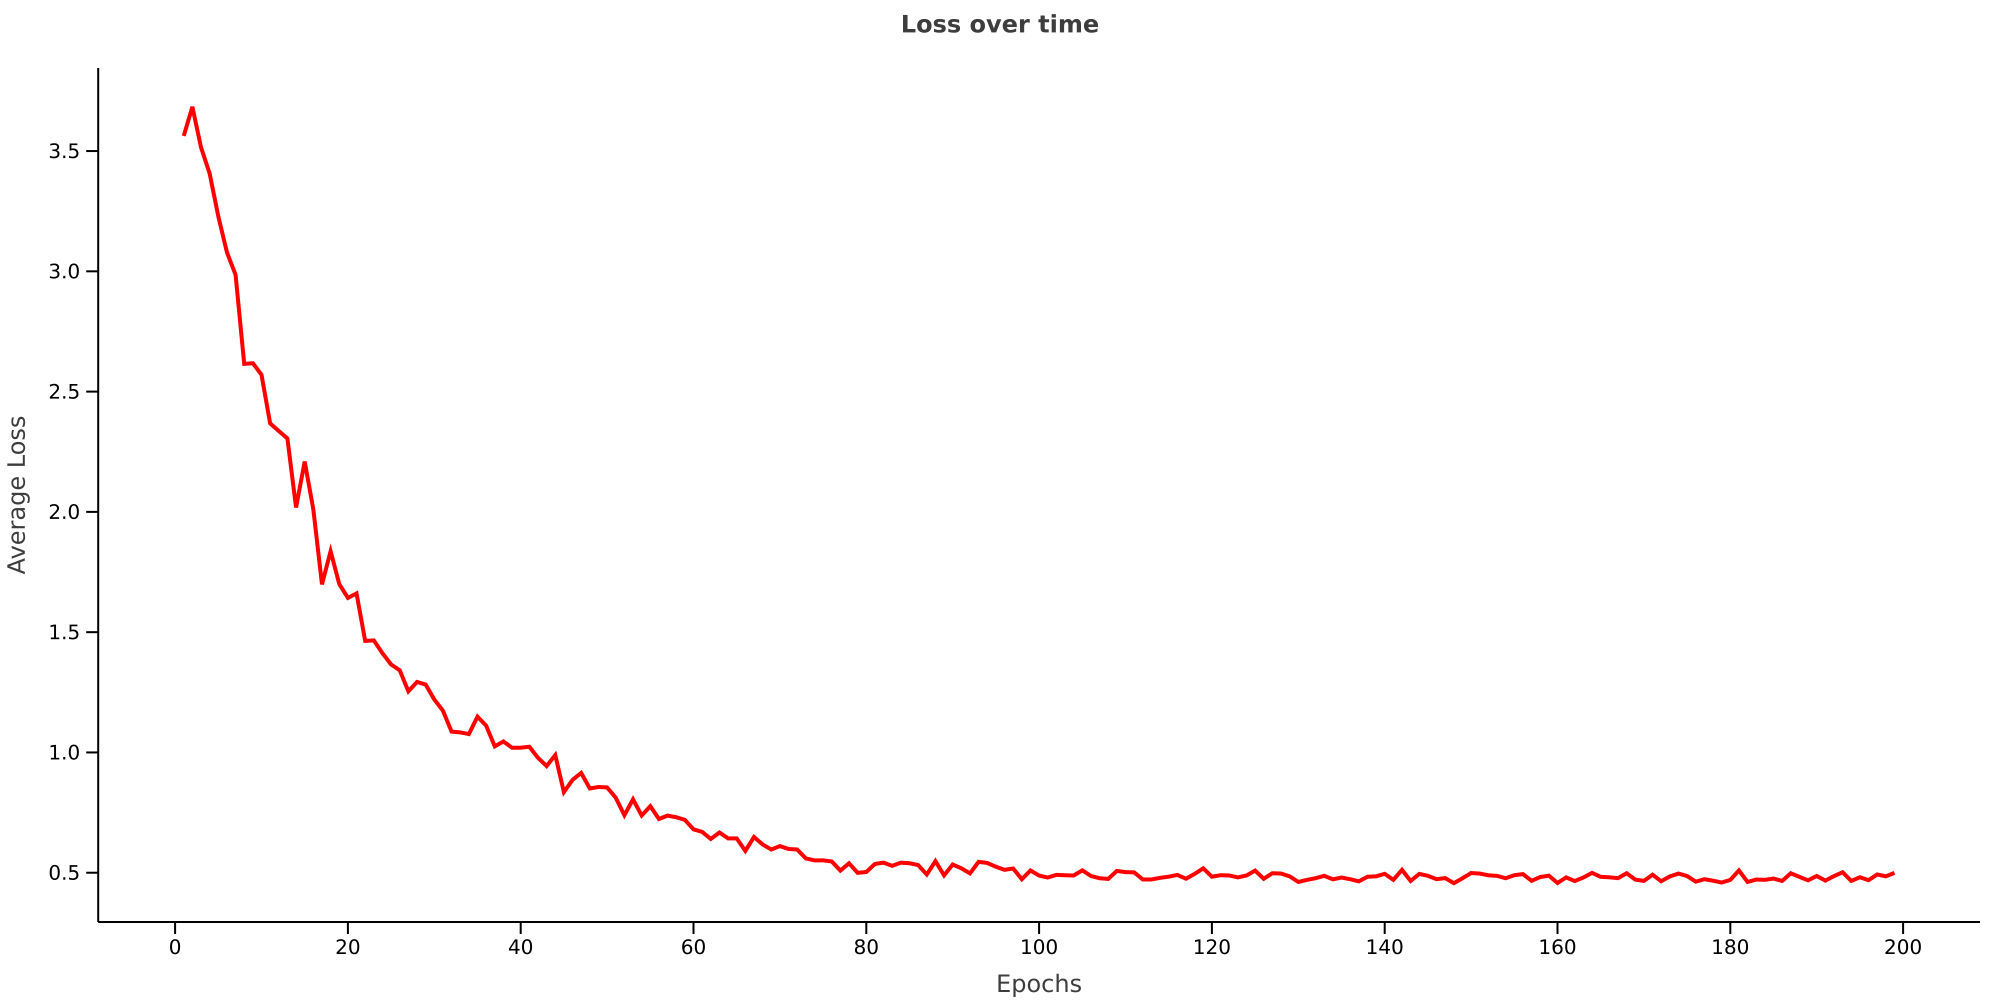
\includegraphics[width=0.70\textwidth]{../figures/training_curve.png}
\caption{Training curve of a single trajectory of gradient descent in parameter space.}
\label{fig:training_curve}
\end{figure}

\begin{table}[H]
\begin{tabular}{ll}
\digraph[scale=0.2]{btree0} {
    graph ["rankdir"="LR","bgcolor"="transparent"];
    "97652294" ["color"="black","fontcolor"="black","fontname"="Helvetica","fontsize"="20","style"="setlinewidth(2)","label"="*"];
    "1027007693" ["color"="black","fontcolor"="black","fontname"="Helvetica","fontsize"="20","style"="setlinewidth(2)","label"="*"];
    "282432134" ["color"="black","fontcolor"="black","fontname"="Helvetica","fontsize"="20","style"="setlinewidth(2)","label"="+"];
    "1282811396" ["color"="black","fontcolor"="black","fontname"="Helvetica","fontsize"="20","style"="setlinewidth(2)","label"="+"];
    "641853239" ["color"="black","fontcolor"="black","fontname"="Helvetica","fontsize"="20","style"="setlinewidth(2)","label"="+"];
    "1920467934" ["color"="black","fontcolor"="black","fontname"="Helvetica","fontsize"="20","style"="setlinewidth(2)","label"="*"];
    "1883840933" ["color"="black","fontcolor"="black","fontname"="Helvetica","fontsize"="20","style"="setlinewidth(2)","label"="*"];
    "233996206" ["color"="black","fontcolor"="black","fontname"="Helvetica","fontsize"="20","style"="setlinewidth(2)","label"="0.307"];
    "x" ["color"="black","fontcolor"="black","fontname"="Helvetica","fontsize"="20","style"="setlinewidth(2)"];
    "614685048" ["color"="black","fontcolor"="black","fontname"="Helvetica","fontsize"="20","style"="setlinewidth(2)","label"="+"];
    "385337537" ["color"="black","fontcolor"="black","fontname"="Helvetica","fontsize"="20","style"="setlinewidth(2)","label"="-"];
    "265119009" ["color"="black","fontcolor"="black","fontname"="Helvetica","fontsize"="20","style"="setlinewidth(2)","label"="*"];
    "832279283" ["color"="black","fontcolor"="black","fontname"="Helvetica","fontsize"="20","style"="setlinewidth(2)","label"="+"];
    "789219251" ["color"="black","fontcolor"="black","fontname"="Helvetica","fontsize"="20","style"="setlinewidth(2)","label"="-"];
    "1375995437" ["color"="black","fontcolor"="black","fontname"="Helvetica","fontsize"="20","style"="setlinewidth(2)","label"="+"];
    "1434041222" ["color"="black","fontcolor"="black","fontname"="Helvetica","fontsize"="20","style"="setlinewidth(2)","label"="+"];
    "838411509" ["color"="black","fontcolor"="black","fontname"="Helvetica","fontsize"="20","style"="setlinewidth(2)","label"="*"];
    "1338841523" ["color"="black","fontcolor"="black","fontname"="Helvetica","fontsize"="20","style"="setlinewidth(2)","label"="-"];
    "802581203" ["color"="black","fontcolor"="black","fontname"="Helvetica","fontsize"="20","style"="setlinewidth(2)","label"="*"];
    "929776179" ["color"="black","fontcolor"="black","fontname"="Helvetica","fontsize"="20","style"="setlinewidth(2)","label"="-"];
    "2050404090" ["color"="black","fontcolor"="black","fontname"="Helvetica","fontsize"="20","style"="setlinewidth(2)","label"="+"];
    "1561408618" ["color"="black","fontcolor"="black","fontname"="Helvetica","fontsize"="20","style"="setlinewidth(2)","label"="+"];
    "668210649" ["color"="black","fontcolor"="black","fontname"="Helvetica","fontsize"="20","style"="setlinewidth(2)","label"="0.355"];
    "1545087375" ["color"="black","fontcolor"="black","fontname"="Helvetica","fontsize"="20","style"="setlinewidth(2)","label"="0.188"];
    "388043093" ["color"="black","fontcolor"="black","fontname"="Helvetica","fontsize"="20","style"="setlinewidth(2)","label"="0.886"];
    "188576144" ["color"="black","fontcolor"="black","fontname"="Helvetica","fontsize"="20","style"="setlinewidth(2)","label"="-1.08"];
    "266437232" ["color"="black","fontcolor"="black","fontname"="Helvetica","fontsize"="20","style"="setlinewidth(2)","label"="0.188"];
    "500772834" ["color"="black","fontcolor"="black","fontname"="Helvetica","fontsize"="20","style"="setlinewidth(2)","label"="1.0"];
    "1691538257" ["color"="black","fontcolor"="black","fontname"="Helvetica","fontsize"="20","style"="setlinewidth(2)","label"="pow"];
    "1335505684" ["color"="black","fontcolor"="black","fontname"="Helvetica","fontsize"="20","style"="setlinewidth(2)","label"="1.555"];
    "1226204845" ["color"="black","fontcolor"="black","fontname"="Helvetica","fontsize"="20","style"="setlinewidth(2)","label"="-"];
    "1" ["color"="black","fontcolor"="black","fontname"="Helvetica","fontsize"="20","style"="setlinewidth(2)","label"="One"];
    "1027007693" -> "97652294" ["color"="blue","arrowhead"="normal","style"="setlinewidth(2)"];
    "282432134" -> "1027007693" ["color"="blue","arrowhead"="normal","style"="setlinewidth(2)"];
    "1282811396" -> "282432134" ["color"="blue","arrowhead"="normal","style"="setlinewidth(2)"];
    "641853239" -> "1282811396" ["color"="blue","arrowhead"="normal","style"="setlinewidth(2)"];
    "1920467934" -> "641853239" ["color"="blue","arrowhead"="normal","style"="setlinewidth(2)"];
    "1883840933" -> "1920467934" ["color"="blue","arrowhead"="normal","style"="setlinewidth(2)"];
    "233996206" -> "1883840933" ["color"="blue","arrowhead"="normal","style"="setlinewidth(2)"];
    "x" -> "1883840933" ["color"="red","arrowhead"="normal","style"="setlinewidth(2)"];
    "x" -> "614685048" ["color"="blue","arrowhead"="normal","style"="setlinewidth(2)"];
    "x" -> "385337537" ["color"="black","arrowhead"="normal","style"="setlinewidth(2)"];
    "x" -> "265119009" ["color"="red","arrowhead"="normal","style"="setlinewidth(2)"];
    "x" -> "1375995437" ["color"="blue","arrowhead"="normal","style"="setlinewidth(2)"];
    "x" -> "1338841523" ["color"="black","arrowhead"="normal","style"="setlinewidth(2)"];
    "x" -> "802581203" ["color"="blue","arrowhead"="normal","style"="setlinewidth(2)"];
    "x" -> "802581203" ["color"="red","arrowhead"="normal","style"="setlinewidth(2)"];
    "x" -> "2050404090" ["color"="blue","arrowhead"="normal","style"="setlinewidth(2)"];
    "614685048" -> "1920467934" ["color"="red","arrowhead"="normal","style"="setlinewidth(2)"];
    "385337537" -> "614685048" ["color"="red","arrowhead"="normal","style"="setlinewidth(2)"];
    "265119009" -> "832279283" ["color"="blue","arrowhead"="normal","style"="setlinewidth(2)"];
    "832279283" -> "789219251" ["color"="black","arrowhead"="normal","style"="setlinewidth(2)"];
    "789219251" -> "641853239" ["color"="red","arrowhead"="normal","style"="setlinewidth(2)"];
    "1375995437" -> "1434041222" ["color"="blue","arrowhead"="normal","style"="setlinewidth(2)"];
    "1434041222" -> "838411509" ["color"="blue","arrowhead"="normal","style"="setlinewidth(2)"];
    "838411509" -> "1282811396" ["color"="red","arrowhead"="normal","style"="setlinewidth(2)"];
    "1338841523" -> "1375995437" ["color"="red","arrowhead"="normal","style"="setlinewidth(2)"];
    "802581203" -> "929776179" ["color"="black","arrowhead"="normal","style"="setlinewidth(2)"];
    "929776179" -> "1434041222" ["color"="red","arrowhead"="normal","style"="setlinewidth(2)"];
    "2050404090" -> "1561408618" ["color"="blue","arrowhead"="normal","style"="setlinewidth(2)"];
    "1561408618" -> "838411509" ["color"="red","arrowhead"="normal","style"="setlinewidth(2)"];
    "668210649" -> "265119009" ["color"="blue","arrowhead"="normal","style"="setlinewidth(2)"];
    "1545087375" -> "832279283" ["color"="red","arrowhead"="normal","style"="setlinewidth(2)"];
    "388043093" -> "2050404090" ["color"="red","arrowhead"="normal","style"="setlinewidth(2)"];
    "188576144" -> "1561408618" ["color"="red","arrowhead"="normal","style"="setlinewidth(2)"];
    "266437232" -> "282432134" ["color"="red","arrowhead"="normal","style"="setlinewidth(2)"];
    "500772834" -> "1027007693" ["color"="red","arrowhead"="normal","style"="setlinewidth(2)"];
    "1691538257" -> "97652294" ["color"="red","arrowhead"="normal","style"="setlinewidth(2)"];
    "1335505684" -> "1691538257" ["color"="blue","arrowhead"="normal","style"="setlinewidth(2)"];
    "1226204845" -> "1691538257" ["color"="red","arrowhead"="normal","style"="setlinewidth(2)"];
    "1" -> "1226204845" ["color"="black","arrowhead"="normal","style"="setlinewidth(2)"];
} & \begin{tikzpicture} \begin{axis}[title={}, width=0.4\textwidth, height=5cm, xlabel=$x$, ylabel=$y$, align=center] \addplot table [mark=none, x index=0, y index=1, col sep=comma] {../data/btree_rand0.csv}; \end{axis} \end{tikzpicture} \\
\digraph[scale=0.2]{btree1} {
    graph ["rankdir"="LR","bgcolor"="transparent"];
    "306115458" ["color"="black","fontcolor"="black","fontname"="Helvetica","fontsize"="20","style"="setlinewidth(2)","label"="*"];
    "944427387" ["color"="black","fontcolor"="black","fontname"="Helvetica","fontsize"="20","style"="setlinewidth(2)","label"="*"];
    "521081105" ["color"="black","fontcolor"="black","fontname"="Helvetica","fontsize"="20","style"="setlinewidth(2)","label"="+"];
    "1907431275" ["color"="black","fontcolor"="black","fontname"="Helvetica","fontsize"="20","style"="setlinewidth(2)","label"="+"];
    "1637061418" ["color"="black","fontcolor"="black","fontname"="Helvetica","fontsize"="20","style"="setlinewidth(2)","label"="+"];
    "1686100174" ["color"="black","fontcolor"="black","fontname"="Helvetica","fontsize"="20","style"="setlinewidth(2)","label"="+"];
    "22671767" ["color"="black","fontcolor"="black","fontname"="Helvetica","fontsize"="20","style"="setlinewidth(2)","label"="+"];
    "2024453272" ["color"="black","fontcolor"="black","fontname"="Helvetica","fontsize"="20","style"="setlinewidth(2)","label"="0.108"];
    "x" ["color"="black","fontcolor"="black","fontname"="Helvetica","fontsize"="20","style"="setlinewidth(2)"];
    "1374026904" ["color"="black","fontcolor"="black","fontname"="Helvetica","fontsize"="20","style"="setlinewidth(2)","label"="*"];
    "536765369" ["color"="black","fontcolor"="black","fontname"="Helvetica","fontsize"="20","style"="setlinewidth(2)","label"="+"];
    "317071334" ["color"="black","fontcolor"="black","fontname"="Helvetica","fontsize"="20","style"="setlinewidth(2)","label"="+"];
    "1224347463" ["color"="black","fontcolor"="black","fontname"="Helvetica","fontsize"="20","style"="setlinewidth(2)","label"="+"];
    "1472465" ["color"="black","fontcolor"="black","fontname"="Helvetica","fontsize"="20","style"="setlinewidth(2)","label"="+"];
    "2129221032" ["color"="black","fontcolor"="black","fontname"="Helvetica","fontsize"="20","style"="setlinewidth(2)","label"="*"];
    "1831477404" ["color"="black","fontcolor"="black","fontname"="Helvetica","fontsize"="20","style"="setlinewidth(2)","label"="+"];
    "1580297332" ["color"="black","fontcolor"="black","fontname"="Helvetica","fontsize"="20","style"="setlinewidth(2)","label"="-"];
    "1966250569" ["color"="black","fontcolor"="black","fontname"="Helvetica","fontsize"="20","style"="setlinewidth(2)","label"="-"];
    "1125381564" ["color"="black","fontcolor"="black","fontname"="Helvetica","fontsize"="20","style"="setlinewidth(2)","label"="+"];
    "370440646" ["color"="black","fontcolor"="black","fontname"="Helvetica","fontsize"="20","style"="setlinewidth(2)","label"="*"];
    "2005733474" ["color"="black","fontcolor"="black","fontname"="Helvetica","fontsize"="20","style"="setlinewidth(2)","label"="-"];
    "511717113" ["color"="black","fontcolor"="black","fontname"="Helvetica","fontsize"="20","style"="setlinewidth(2)","label"="+"];
    "98394724" ["color"="black","fontcolor"="black","fontname"="Helvetica","fontsize"="20","style"="setlinewidth(2)","label"="-0.64"];
    "2085002312" ["color"="black","fontcolor"="black","fontname"="Helvetica","fontsize"="20","style"="setlinewidth(2)","label"="0.186"];
    "1791045777" ["color"="black","fontcolor"="black","fontname"="Helvetica","fontsize"="20","style"="setlinewidth(2)","label"="0.308"];
    "2130772866" ["color"="black","fontcolor"="black","fontname"="Helvetica","fontsize"="20","style"="setlinewidth(2)","label"="0.638"];
    "728739494" ["color"="black","fontcolor"="black","fontname"="Helvetica","fontsize"="20","style"="setlinewidth(2)","label"="0.119"];
    "1237550792" ["color"="black","fontcolor"="black","fontname"="Helvetica","fontsize"="20","style"="setlinewidth(2)","label"="0.518"];
    "1712943792" ["color"="black","fontcolor"="black","fontname"="Helvetica","fontsize"="20","style"="setlinewidth(2)","label"="1.0"];
    "842741472" ["color"="black","fontcolor"="black","fontname"="Helvetica","fontsize"="20","style"="setlinewidth(2)","label"="pow"];
    "1766505436" ["color"="black","fontcolor"="black","fontname"="Helvetica","fontsize"="20","style"="setlinewidth(2)","label"="2.930"];
    "1164440413" ["color"="black","fontcolor"="black","fontname"="Helvetica","fontsize"="20","style"="setlinewidth(2)","label"="-"];
    "1" ["color"="black","fontcolor"="black","fontname"="Helvetica","fontsize"="20","style"="setlinewidth(2)","label"="One"];
    "944427387" -> "306115458" ["color"="blue","arrowhead"="normal","style"="setlinewidth(2)"];
    "521081105" -> "944427387" ["color"="blue","arrowhead"="normal","style"="setlinewidth(2)"];
    "1907431275" -> "521081105" ["color"="blue","arrowhead"="normal","style"="setlinewidth(2)"];
    "1637061418" -> "1907431275" ["color"="blue","arrowhead"="normal","style"="setlinewidth(2)"];
    "1686100174" -> "1637061418" ["color"="blue","arrowhead"="normal","style"="setlinewidth(2)"];
    "22671767" -> "1686100174" ["color"="blue","arrowhead"="normal","style"="setlinewidth(2)"];
    "2024453272" -> "22671767" ["color"="blue","arrowhead"="normal","style"="setlinewidth(2)"];
    "x" -> "22671767" ["color"="red","arrowhead"="normal","style"="setlinewidth(2)"];
    "x" -> "1374026904" ["color"="red","arrowhead"="normal","style"="setlinewidth(2)"];
    "x" -> "317071334" ["color"="blue","arrowhead"="normal","style"="setlinewidth(2)"];
    "x" -> "317071334" ["color"="red","arrowhead"="normal","style"="setlinewidth(2)"];
    "x" -> "1224347463" ["color"="red","arrowhead"="normal","style"="setlinewidth(2)"];
    "x" -> "1831477404" ["color"="blue","arrowhead"="normal","style"="setlinewidth(2)"];
    "x" -> "1966250569" ["color"="black","arrowhead"="normal","style"="setlinewidth(2)"];
    "x" -> "1125381564" ["color"="blue","arrowhead"="normal","style"="setlinewidth(2)"];
    "x" -> "2005733474" ["color"="black","arrowhead"="normal","style"="setlinewidth(2)"];
    "1374026904" -> "536765369" ["color"="blue","arrowhead"="normal","style"="setlinewidth(2)"];
    "536765369" -> "1637061418" ["color"="red","arrowhead"="normal","style"="setlinewidth(2)"];
    "317071334" -> "536765369" ["color"="red","arrowhead"="normal","style"="setlinewidth(2)"];
    "1224347463" -> "1472465" ["color"="blue","arrowhead"="normal","style"="setlinewidth(2)"];
    "1472465" -> "2129221032" ["color"="blue","arrowhead"="normal","style"="setlinewidth(2)"];
    "2129221032" -> "1907431275" ["color"="red","arrowhead"="normal","style"="setlinewidth(2)"];
    "1831477404" -> "1580297332" ["color"="black","arrowhead"="normal","style"="setlinewidth(2)"];
    "1580297332" -> "1472465" ["color"="red","arrowhead"="normal","style"="setlinewidth(2)"];
    "1966250569" -> "1831477404" ["color"="red","arrowhead"="normal","style"="setlinewidth(2)"];
    "1125381564" -> "370440646" ["color"="blue","arrowhead"="normal","style"="setlinewidth(2)"];
    "370440646" -> "2129221032" ["color"="red","arrowhead"="normal","style"="setlinewidth(2)"];
    "2005733474" -> "511717113" ["color"="red","arrowhead"="normal","style"="setlinewidth(2)"];
    "511717113" -> "370440646" ["color"="red","arrowhead"="normal","style"="setlinewidth(2)"];
    "98394724" -> "1686100174" ["color"="red","arrowhead"="normal","style"="setlinewidth(2)"];
    "2085002312" -> "1374026904" ["color"="blue","arrowhead"="normal","style"="setlinewidth(2)"];
    "1791045777" -> "1224347463" ["color"="blue","arrowhead"="normal","style"="setlinewidth(2)"];
    "2130772866" -> "1125381564" ["color"="red","arrowhead"="normal","style"="setlinewidth(2)"];
    "728739494" -> "511717113" ["color"="blue","arrowhead"="normal","style"="setlinewidth(2)"];
    "1237550792" -> "521081105" ["color"="red","arrowhead"="normal","style"="setlinewidth(2)"];
    "1712943792" -> "944427387" ["color"="red","arrowhead"="normal","style"="setlinewidth(2)"];
    "842741472" -> "306115458" ["color"="red","arrowhead"="normal","style"="setlinewidth(2)"];
    "1766505436" -> "842741472" ["color"="blue","arrowhead"="normal","style"="setlinewidth(2)"];
    "1164440413" -> "842741472" ["color"="red","arrowhead"="normal","style"="setlinewidth(2)"];
    "1" -> "1164440413" ["color"="black","arrowhead"="normal","style"="setlinewidth(2)"];
} & \begin{tikzpicture} \begin{axis}[title={}, width=0.4\textwidth, height=5cm, xlabel=$x$, ylabel=$y$, align=center] \addplot table [mark=none, x index=0, y index=1, col sep=comma] {../data/btree_rand1.csv}; \end{axis} \end{tikzpicture} \\
\digraph[scale=0.2]{btree2} {
    graph ["rankdir"="LR","bgcolor"="transparent"];
    "1007412025" ["color"="black","fontcolor"="black","fontname"="Helvetica","fontsize"="20","style"="setlinewidth(2)","label"="*"];
    "2053591126" ["color"="black","fontcolor"="black","fontname"="Helvetica","fontsize"="20","style"="setlinewidth(2)","label"="*"];
    "231756373" ["color"="black","fontcolor"="black","fontname"="Helvetica","fontsize"="20","style"="setlinewidth(2)","label"="+"];
    "887750041" ["color"="black","fontcolor"="black","fontname"="Helvetica","fontsize"="20","style"="setlinewidth(2)","label"="+"];
    "1010953501" ["color"="black","fontcolor"="black","fontname"="Helvetica","fontsize"="20","style"="setlinewidth(2)","label"="+"];
    "1423561005" ["color"="black","fontcolor"="black","fontname"="Helvetica","fontsize"="20","style"="setlinewidth(2)","label"="+"];
    "943870983" ["color"="black","fontcolor"="black","fontname"="Helvetica","fontsize"="20","style"="setlinewidth(2)","label"="+"];
    "x" ["color"="black","fontcolor"="black","fontname"="Helvetica","fontsize"="20","style"="setlinewidth(2)"];
    "1084502906" ["color"="black","fontcolor"="black","fontname"="Helvetica","fontsize"="20","style"="setlinewidth(2)","label"="-"];
    "1881561036" ["color"="black","fontcolor"="black","fontname"="Helvetica","fontsize"="20","style"="setlinewidth(2)","label"="+"];
    "52908367" ["color"="black","fontcolor"="black","fontname"="Helvetica","fontsize"="20","style"="setlinewidth(2)","label"="*"];
    "1279271200" ["color"="black","fontcolor"="black","fontname"="Helvetica","fontsize"="20","style"="setlinewidth(2)","label"="-"];
    "587153993" ["color"="black","fontcolor"="black","fontname"="Helvetica","fontsize"="20","style"="setlinewidth(2)","label"="+"];
    "1613095350" ["color"="black","fontcolor"="black","fontname"="Helvetica","fontsize"="20","style"="setlinewidth(2)","label"="-"];
    "1971764991" ["color"="black","fontcolor"="black","fontname"="Helvetica","fontsize"="20","style"="setlinewidth(2)","label"="+"];
    "1276261147" ["color"="black","fontcolor"="black","fontname"="Helvetica","fontsize"="20","style"="setlinewidth(2)","label"="+"];
    "18242360" ["color"="black","fontcolor"="black","fontname"="Helvetica","fontsize"="20","style"="setlinewidth(2)","label"="*"];
    "1527953000" ["color"="black","fontcolor"="black","fontname"="Helvetica","fontsize"="20","style"="setlinewidth(2)","label"="-"];
    "135640095" ["color"="black","fontcolor"="black","fontname"="Helvetica","fontsize"="20","style"="setlinewidth(2)","label"="*"];
    "1632682988" ["color"="black","fontcolor"="black","fontname"="Helvetica","fontsize"="20","style"="setlinewidth(2)","label"="*"];
    "359922172" ["color"="black","fontcolor"="black","fontname"="Helvetica","fontsize"="20","style"="setlinewidth(2)","label"="+"];
    "1136419747" ["color"="black","fontcolor"="black","fontname"="Helvetica","fontsize"="20","style"="setlinewidth(2)","label"="0.375"];
    "1785507932" ["color"="black","fontcolor"="black","fontname"="Helvetica","fontsize"="20","style"="setlinewidth(2)","label"="0.791"];
    "757004314" ["color"="black","fontcolor"="black","fontname"="Helvetica","fontsize"="20","style"="setlinewidth(2)","label"="1.261"];
    "996796369" ["color"="black","fontcolor"="black","fontname"="Helvetica","fontsize"="20","style"="setlinewidth(2)","label"="-0.65"];
    "1430439149" ["color"="black","fontcolor"="black","fontname"="Helvetica","fontsize"="20","style"="setlinewidth(2)","label"="0.236"];
    "1153447573" ["color"="black","fontcolor"="black","fontname"="Helvetica","fontsize"="20","style"="setlinewidth(2)","label"="0.494"];
    "1786294176" ["color"="black","fontcolor"="black","fontname"="Helvetica","fontsize"="20","style"="setlinewidth(2)","label"="-0.23"];
    "2082351774" ["color"="black","fontcolor"="black","fontname"="Helvetica","fontsize"="20","style"="setlinewidth(2)","label"="1.0"];
    "1730704097" ["color"="black","fontcolor"="black","fontname"="Helvetica","fontsize"="20","style"="setlinewidth(2)","label"="pow"];
    "1062635358" ["color"="black","fontcolor"="black","fontname"="Helvetica","fontsize"="20","style"="setlinewidth(2)","label"="3.506"];
    "265321659" ["color"="black","fontcolor"="black","fontname"="Helvetica","fontsize"="20","style"="setlinewidth(2)","label"="-"];
    "1" ["color"="black","fontcolor"="black","fontname"="Helvetica","fontsize"="20","style"="setlinewidth(2)","label"="One"];
    "2053591126" -> "1007412025" ["color"="blue","arrowhead"="normal","style"="setlinewidth(2)"];
    "231756373" -> "2053591126" ["color"="blue","arrowhead"="normal","style"="setlinewidth(2)"];
    "887750041" -> "231756373" ["color"="blue","arrowhead"="normal","style"="setlinewidth(2)"];
    "1010953501" -> "887750041" ["color"="blue","arrowhead"="normal","style"="setlinewidth(2)"];
    "1423561005" -> "1010953501" ["color"="blue","arrowhead"="normal","style"="setlinewidth(2)"];
    "943870983" -> "1423561005" ["color"="blue","arrowhead"="normal","style"="setlinewidth(2)"];
    "x" -> "943870983" ["color"="blue","arrowhead"="normal","style"="setlinewidth(2)"];
    "x" -> "1084502906" ["color"="black","arrowhead"="normal","style"="setlinewidth(2)"];
    "x" -> "52908367" ["color"="blue","arrowhead"="normal","style"="setlinewidth(2)"];
    "x" -> "52908367" ["color"="red","arrowhead"="normal","style"="setlinewidth(2)"];
    "x" -> "1971764991" ["color"="blue","arrowhead"="normal","style"="setlinewidth(2)"];
    "x" -> "135640095" ["color"="blue","arrowhead"="normal","style"="setlinewidth(2)"];
    "x" -> "1632682988" ["color"="blue","arrowhead"="normal","style"="setlinewidth(2)"];
    "x" -> "1632682988" ["color"="red","arrowhead"="normal","style"="setlinewidth(2)"];
    "1084502906" -> "1881561036" ["color"="red","arrowhead"="normal","style"="setlinewidth(2)"];
    "1881561036" -> "1423561005" ["color"="red","arrowhead"="normal","style"="setlinewidth(2)"];
    "52908367" -> "1279271200" ["color"="black","arrowhead"="normal","style"="setlinewidth(2)"];
    "1279271200" -> "587153993" ["color"="red","arrowhead"="normal","style"="setlinewidth(2)"];
    "587153993" -> "1613095350" ["color"="black","arrowhead"="normal","style"="setlinewidth(2)"];
    "1613095350" -> "1010953501" ["color"="red","arrowhead"="normal","style"="setlinewidth(2)"];
    "1971764991" -> "1276261147" ["color"="blue","arrowhead"="normal","style"="setlinewidth(2)"];
    "1276261147" -> "18242360" ["color"="blue","arrowhead"="normal","style"="setlinewidth(2)"];
    "18242360" -> "1527953000" ["color"="black","arrowhead"="normal","style"="setlinewidth(2)"];
    "1527953000" -> "887750041" ["color"="red","arrowhead"="normal","style"="setlinewidth(2)"];
    "135640095" -> "1276261147" ["color"="red","arrowhead"="normal","style"="setlinewidth(2)"];
    "1632682988" -> "359922172" ["color"="blue","arrowhead"="normal","style"="setlinewidth(2)"];
    "359922172" -> "18242360" ["color"="red","arrowhead"="normal","style"="setlinewidth(2)"];
    "1136419747" -> "943870983" ["color"="red","arrowhead"="normal","style"="setlinewidth(2)"];
    "1785507932" -> "1881561036" ["color"="blue","arrowhead"="normal","style"="setlinewidth(2)"];
    "757004314" -> "587153993" ["color"="blue","arrowhead"="normal","style"="setlinewidth(2)"];
    "996796369" -> "1971764991" ["color"="red","arrowhead"="normal","style"="setlinewidth(2)"];
    "1430439149" -> "135640095" ["color"="red","arrowhead"="normal","style"="setlinewidth(2)"];
    "1153447573" -> "359922172" ["color"="red","arrowhead"="normal","style"="setlinewidth(2)"];
    "1786294176" -> "231756373" ["color"="red","arrowhead"="normal","style"="setlinewidth(2)"];
    "2082351774" -> "2053591126" ["color"="red","arrowhead"="normal","style"="setlinewidth(2)"];
    "1730704097" -> "1007412025" ["color"="red","arrowhead"="normal","style"="setlinewidth(2)"];
    "1062635358" -> "1730704097" ["color"="blue","arrowhead"="normal","style"="setlinewidth(2)"];
    "265321659" -> "1730704097" ["color"="red","arrowhead"="normal","style"="setlinewidth(2)"];
    "1" -> "265321659" ["color"="black","arrowhead"="normal","style"="setlinewidth(2)"];
} & \begin{tikzpicture} \begin{axis}[title={}, width=0.4\textwidth, height=5cm, xlabel=$x$, ylabel=$y$, align=center] \addplot table [mark=none, x index=0, y index=1, col sep=comma] {../data/btree_rand2.csv}; \end{axis} \end{tikzpicture}
\end{tabular}
\caption{\label{tab:btrees} Some DFGs generated by \autoref{eq:btree_gen} with accompanying 2D plots.}
\end{table}

\begin{figure}
\begin{tikzpicture} \begin{axis}[title={Average Errors per 1k Evaluations for Random Sampling Strategy}, width=\textwidth, height=5cm, xlabel=$\text{Error threshold}$, ylabel=$\text{Errors/eval}$, align=center] \addplot table [mark=none, x index=0, y index=1, col sep=comma] {../data/urand_eff0.csv}; \end{axis} \end{tikzpicture} \\
\end{figure}

\begin{kotlinlisting}
val model = Vec(D30) { x pow (it + 1) } dot weights
var update = Vec(D30) { 0.0 }

batches.forEach { i, batch ->
  val batchInputs = arrayOf(xBatchIn to batch.first, label to batch.second)
  val batchLoss = squaredLoss(batchInputs)
  val weightGrads = batchLoss.d(theta)(*newWeights)
  update = beta * update + (1 - beta) * weightGrads
  newWeights = newWeights - alpha * update
}

val adModel = decodePolynomial(newWeights)
val surrogateLoss = (model - adModel) pow 2
\end{kotlinlisting}

Our adversary takes as input the original the regression model $\hat{f}$, a set of new IO pairs from the same expression, and resumes the original training procedure on the $\hat{f}$ using the supplied datapoints for a fixed number of epochs, $E$, to produce a new model $\hat{f}'$. $\hat{f}'$ is used to construct a surrogate loss $\hat\mathcal{L}(x) = (\hat{f}(x) - \hat{f}'(x))^2$, which can be maximized using \autoref{alg:diff_adversary}. We report the efficiency of the adversarial testing strategy for various error thresholds in terms of standard deviations from the mean squared error on the true loss function $\mathcal{L}(x) = (f(x) - f'(x))$. On average, the adversary yields a $10-15\%$ improvement over random search.

\begin{figure}
\begin{tikzpicture}
\begin{axis}[title={Average efficiency in terms of standard deviations over MSE}, width=\textwidth, height=10cm, xlabel=$\sigma$, ylabel=Average errors detected per labeled input, legend pos=north east, align=center, xtick distance=0.5]
\addplot+[error bars/.cd, y dir = both, y explicit, every nth mark=5] table [mark=none, x index=0, y index=1, y error index=2, col sep=comma] {../data/seff.csv};
\addlegendentry{Probabilistic Generator}
\addplot+[error bars/.cd, y dir = both, y explicit, every nth mark=5] table [mark=none, x index=0, y index=3, y error index=4, col sep=comma] {../data/seff.csv};
\addlegendentry{Differential Adversary}
\end{axis}
\end{tikzpicture}
\caption{By construction, the differential shrinker detects more errors per IO example.}
\label{fig:pbt_comparison}
\end{figure}

violations for exceeding threshold
compare baseline w.r.t. finding
leave out intervals, search to find regions. compare # of samples

\section{Conclusion}

In this chapter we have visited some interesting ideas for validating intelligent systems from the perspective of software engineering and machine learning. We have seen a curious resemblance between some new and old ideas in adversarial learning and fuzz testing. We have proposed a framework for evaluating differentiable programs in a low-cost, data-driven manner and suggest some intriguing directions for future research.

\begin{figure}
\centering
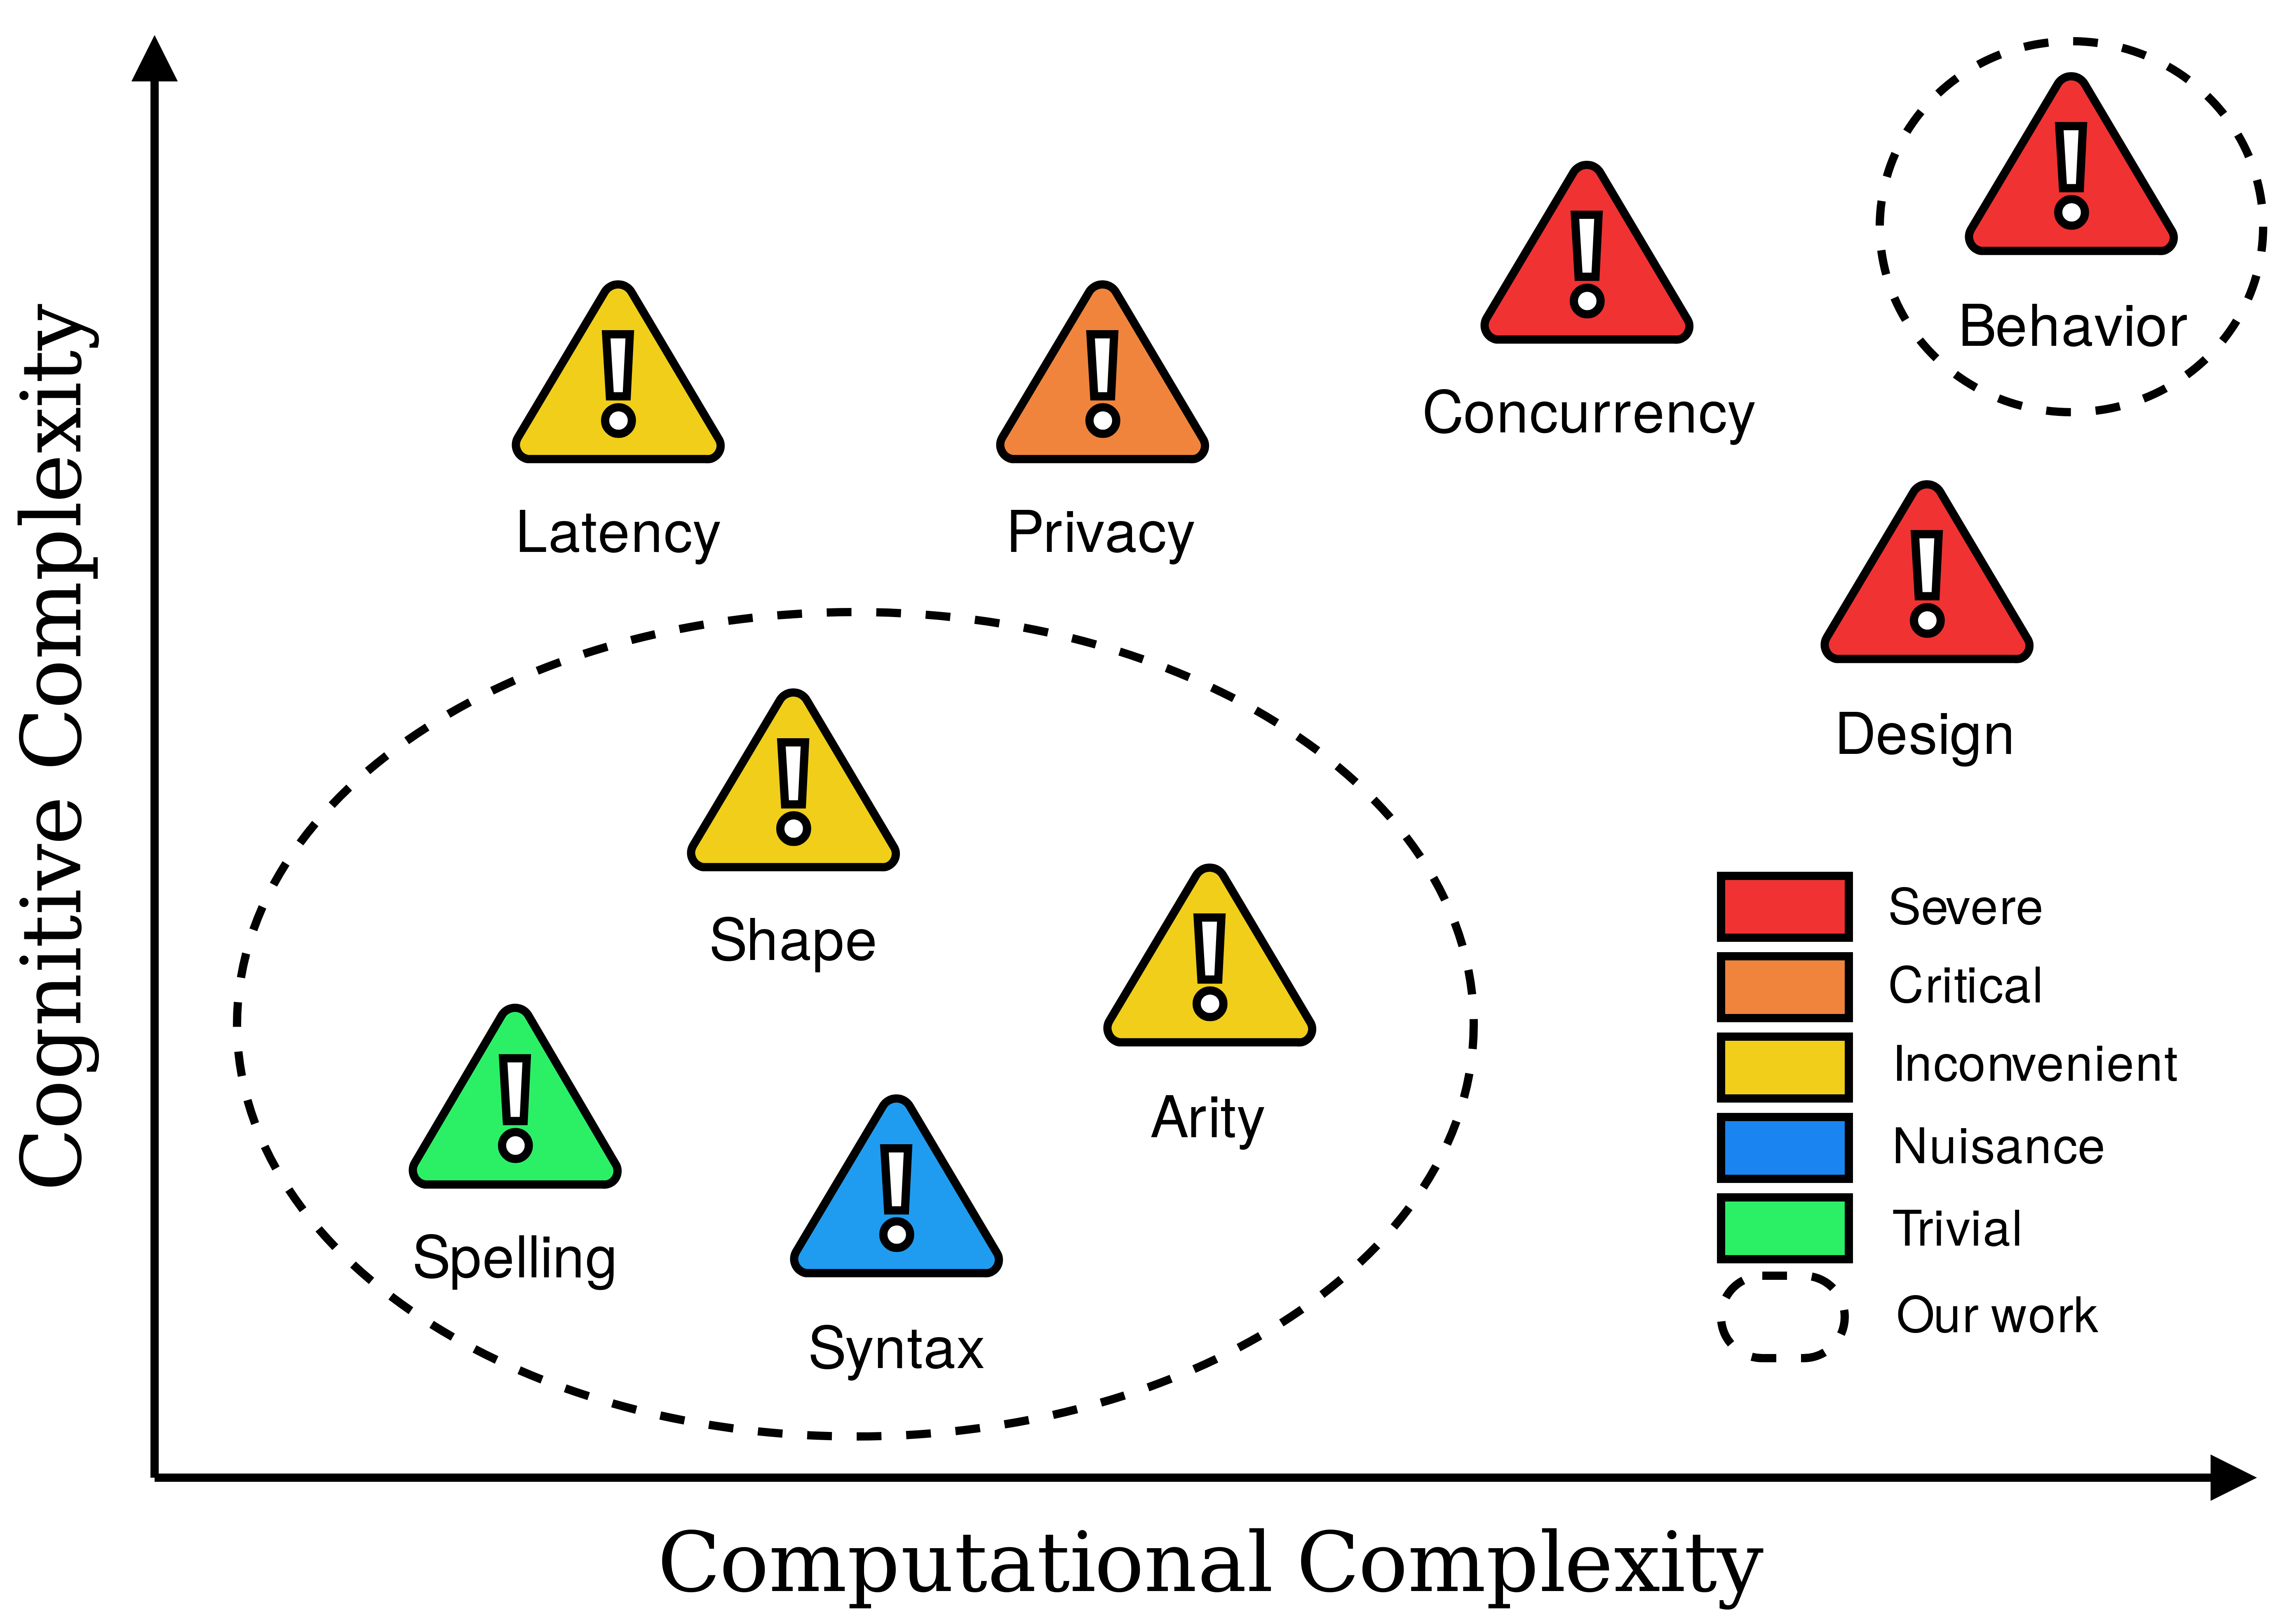
\includegraphics[width=0.60\textwidth]{../figures/verification_complexity.png}
\caption{Complexity of detecting various types of programming errors.}
\label{fig:verification_complexity}
\end{figure}

Type systems, compilers and fuzzers are all part of a broader class of validation and verification tools. The goal of these tools is to provide feedback as early as possible. Some errors (e.g. syntactical errors), are minor nuisances and can be quickly detected with a good incremental parser (\autoref{subsec:the-parser}). Others, as shown in~\autoref{fig:verification_complexity}, are more complex but can be detected by spending computation. We argue this computational cost is often justified as undetected bugs can have catastrophic consequences. Spending computation frees up valuable cognitive resources better spent on more challenging tasks downstream. Studies have shown bugs detected early in development are more likely to be fixed~\citep{distefano2019scaling} -- saving minutes in development could save lives during operation.

Learning capabilities will play a crucial role in autonomous systems. As today's engineers begin to incorporate learning in tomorrow's safety-critical robotic systems, we believe the increased assurance provided by intelligent validation and verification tools will be indispensable for the widespread deployment of these complex adaptive cyberphysical systems.


\chapter{Outils pour la robotique reproductible}\label{ch:ducker}

\setlength{\epigraphwidth}{0.93\textwidth}
\epigraph{La seule façon de réaliser des progrès substantiels dans un domaine quelconque est de s'appuyer sur le travail des autres. Pourtant, la programmation informatique reste une industrie artisanale car les programmeurs insistent pour réinventer des programmes pour chaque nouvelle application, au lieu d'utiliser ce qui existe déjà. Nous devons encourager une manière de regrouper les programmes de manière à ce qu'ils puissent être perçus comme des outils standard, chacun accomplissant sa tâche spécialisée suffisamment bien et s'interfacant avec d'autres outils de manière si pratique que les programmeurs ressentent rarement le besoin de créer leur propre version à partir de zéro.''}{\begin{flushright}--\citet{kernighan1976software}, \href{https://dl.acm.org/doi/10.1145/1010726.1010728}{\textit{Software tools}}\end{flushright}}

Dans ce chapitre, nous abordons le défi de la reproductibilité des logiciels et la manière dont les meilleures pratiques du génie logiciel, telles que les outils d'intégration continue et de conteneurisation, peuvent aider les chercheurs à atténuer la variabilité associée à la construction et à la maintenance des logiciels de robotique. D'une manière générale, nos travaux tentent d'isoler les sources de variabilité computationnelle, et n'envisagent pas les notions de variabilité statistique découlant de l'incertitude aléatoire ou épistémique~\citep{diaz2018interactive}. Cependant, la réduction de la variabilité informatique (qui entrave souvent la reproductibilité expérimentale) est une étape clé pour permettre aux chercheurs d'identifier et de diagnostiquer plus rapidement ces variables plus insaisissables en robotique et en apprentissage machine.

Afin d'aborder la question de la reproductibilité des logiciels, nous avons rassemblé un ensemble d'outils et de flux de développement représentant les meilleures pratiques en matière de génie logiciel. Ces outils sont principalement basés sur la \textit{containerisation}, une technologie de virtualisation largement adoptée dans l'industrie du logiciel. Pour abaisser la barrière d'entrée pour les nouveaux contributeurs et minimiser la variabilité entre les plates-formes matérielles, nous avons développé une infrastructure de conteneurs de pointe basée sur Docker~\citep{merkel2014docker}, un moteur de conteneurs très populaire. Docker permet aux utilisateurs de mettre en place des artefacts de déploiement versionnés qui figent efficacement un système de fichiers entier, et de gérer les contraintes de ressources via un environnement d'exécution en "sandboxed".

Le contenu de ce chapitre est organisé comme suit. Dans \autoref{sec:dependency-management} nous introduisons le problème de la résolution des dépendances et le défi de la construction d'artefacts logiciels reproductibles. Dans \autoref{sec:os-and-virtualization}, nous décrivons une solution générale à ce problème, la virtualisation des logiciels. Ensuite, dans \autoref{sec:containerization}, nous discutons d'une approche légère de la virtualisation, connue sous le nom de conteneurisation. Dans \autoref{sec:docker-intro}, nous faisons une visite guidée à travers une implémentation de conteneur, appelée Docker. Enfin, dans \autoref{sec:ros-docker}, nous présentons DuckieOS, un environnement dockerisé pour la construction d'applications robotiques reproductibles pour la recherche et l'utilisation pédagogique.

\section{Dependency management}\label{sec:dependency-management}

Une source commune de variabilité dans le développement de logiciels est la dépendance des logiciels. Pendant de nombreuses années, les développeurs ont eu du mal à gérer les dépendances avant qu'on ne découvre que le problème de résolution des dépendances était NP-complete~\citep{abate2012dependency}. Si nous supposons qu'aucune version de la même dépendance ne peut être installée simultanément, alors pour un ensemble donné de logiciels qui doivent être installés, et de dépendances nécessaires pour les installer, la détermination de la version cohérente la plus récente des dépendances est aussi difficile que les problèmes les plus difficiles de NP. Officieusement, ce problème est connu sous le nom de \textit{dependency hell} et devient de plus en plus problématique à mesure que les projets logiciels se développent et introduisent de nouvelles dépendances.

L'enfer des dépendances ne se produit pas seulement à l'intérieur des projets logiciels individuels, mais aussi à travers les projets et les environnements de développement. Des centaines de gestionnaires de paquets ont été développés pour divers systèmes d'exploitation, langages de programmation et cadres de développement. Ubuntu dispose du \href{https://help.ubuntu.com/lts/serverguide/apt.html}{Advanced Package Tool} (\inline{apt}), macOS a \href{https://brew.sh/}{Homebrew} (\inline{brew}), Windows a \href{https://chocolatey.org/}{Chocolatey} (\inline{choco}). La plupart des écosystèmes de langage de programmation ont leurs propres gestionnaires de paquets sur mesure ; \href{https://conan.io/}{Conan} pour C/C++, \href{https://maven.apache.org}{Maven} pour Java, et \href{https://www.haskell.org/cabal/}{Cabal} pour Haskell. Python a développé de nombreuses solutions qui se chevauchent pour la gestion des paquets, notamment \href{https://pypi.org/project/pip/}{pip}, \href{https://www.anaconda.com/}{Anaconda}, \href{https://github.com/pyenv/pyenv}{PyEnv}, \href{https://virtualenv.pypa.io/}{Virtualenv}, et d'autres. Certains d'entre eux installent des paquets pour l'ensemble du système, et d'autres fournissent des environnements en ligne de commande. Au cours de la vie d'un système informatique, à mesure que les paquets sont installés et partiellement supprimés, il devient difficile de suivre les changements et leurs effets secondaires.

Le problème provient essentiellement de l'exigence selon laquelle aucune version de la même dépendance ne peut être installée simultanément. En outre, les installateurs de logiciels ont tendance à pulvériser des fichiers dans le système de fichiers, qui peuvent être corrompus et sont difficiles à supprimer complètement si le besoin s'en fait sentir. Pour résoudre ces problèmes, il faut une certaine notion de "contrôle", de sorte que lorsqu'un nouveau logiciel est installé, toute modification ultérieure puisse être retracée et annulée. Des sauvegardes matérielles feraient l'affaire, mais elles sont lourdes à gérer et ne conviennent pas à des fins de développement. Il serait plutôt pratique de disposer d'un outil permettant aux applications de créer un système de fichiers privé, d'installer leurs dépendances et d'éviter de contaminer le système d'exploitation hôte.

\section{Operating systems and virtualization}\label{sec:os-and-virtualization}

Avec la croissance des opérations de développement (devops), un certain nombre de solutions ont émergé pour la construction et l'exécution d'artefacts logiciels génériques. La plupart de ces solutions sont des émulateurs, qui simulent complètement une architecture de processeur étrangère, et donc tout logiciel qui s'exécute sur celle-ci. Une autre solution est celle des machines virtuelles (VM), une sorte d'environnement d'exécution isolé qui utilise un \textit{hypervisor} pour faciliter l'accès au matériel, mais qui fonctionne généralement sur du métal nu. L'inconvénient de ces deux méthodes est leur efficacité. Les machines virtuelles contiennent des systèmes d'exploitation à part entière et sont donc lourdes à exécuter et à déboguer. Cela est particulièrement inutile pour construire et exécuter une petite application sur un système d'exploitation étranger. Les émulateurs fonctionnent beaucoup plus lentement que le code machine natif, selon les architectures hôte et cible.

En 2006, Linux a introduit plusieurs nouvelles fonctionnalités du noyau pour contrôler des groupes de processus, sous l'égide de \textbf{cgroups}~\citep{menage2007adding}. Collectivement, ces fonctionnalités prennent en charge une forme de virtualisation légère, présentant de nombreux avantages des machines virtuelles (VM) tels que le contrôle des ressources et l'isolation de l'espace de noms, sans les surcharges de calcul associées à la virtualisation complète. Ces fonctionnalités ont ouvert la voie à un ensemble d'outils qui sont aujourd'hui connus sous le nom de conteneurs. Contrairement aux machines virtuelles, les conteneurs partagent un noyau commun, mais restent isolés de leur système d'exploitation hôte et des conteneurs frères et sœurs. Alors que les machines virtuelles nécessitent souvent du matériel de type serveur pour fonctionner correctement, les conteneurs conviennent à une catégorie beaucoup plus large de plateformes mobiles et embarquées en raison de leur faible empreinte sur les ressources.

\begin{figure}
\centrer
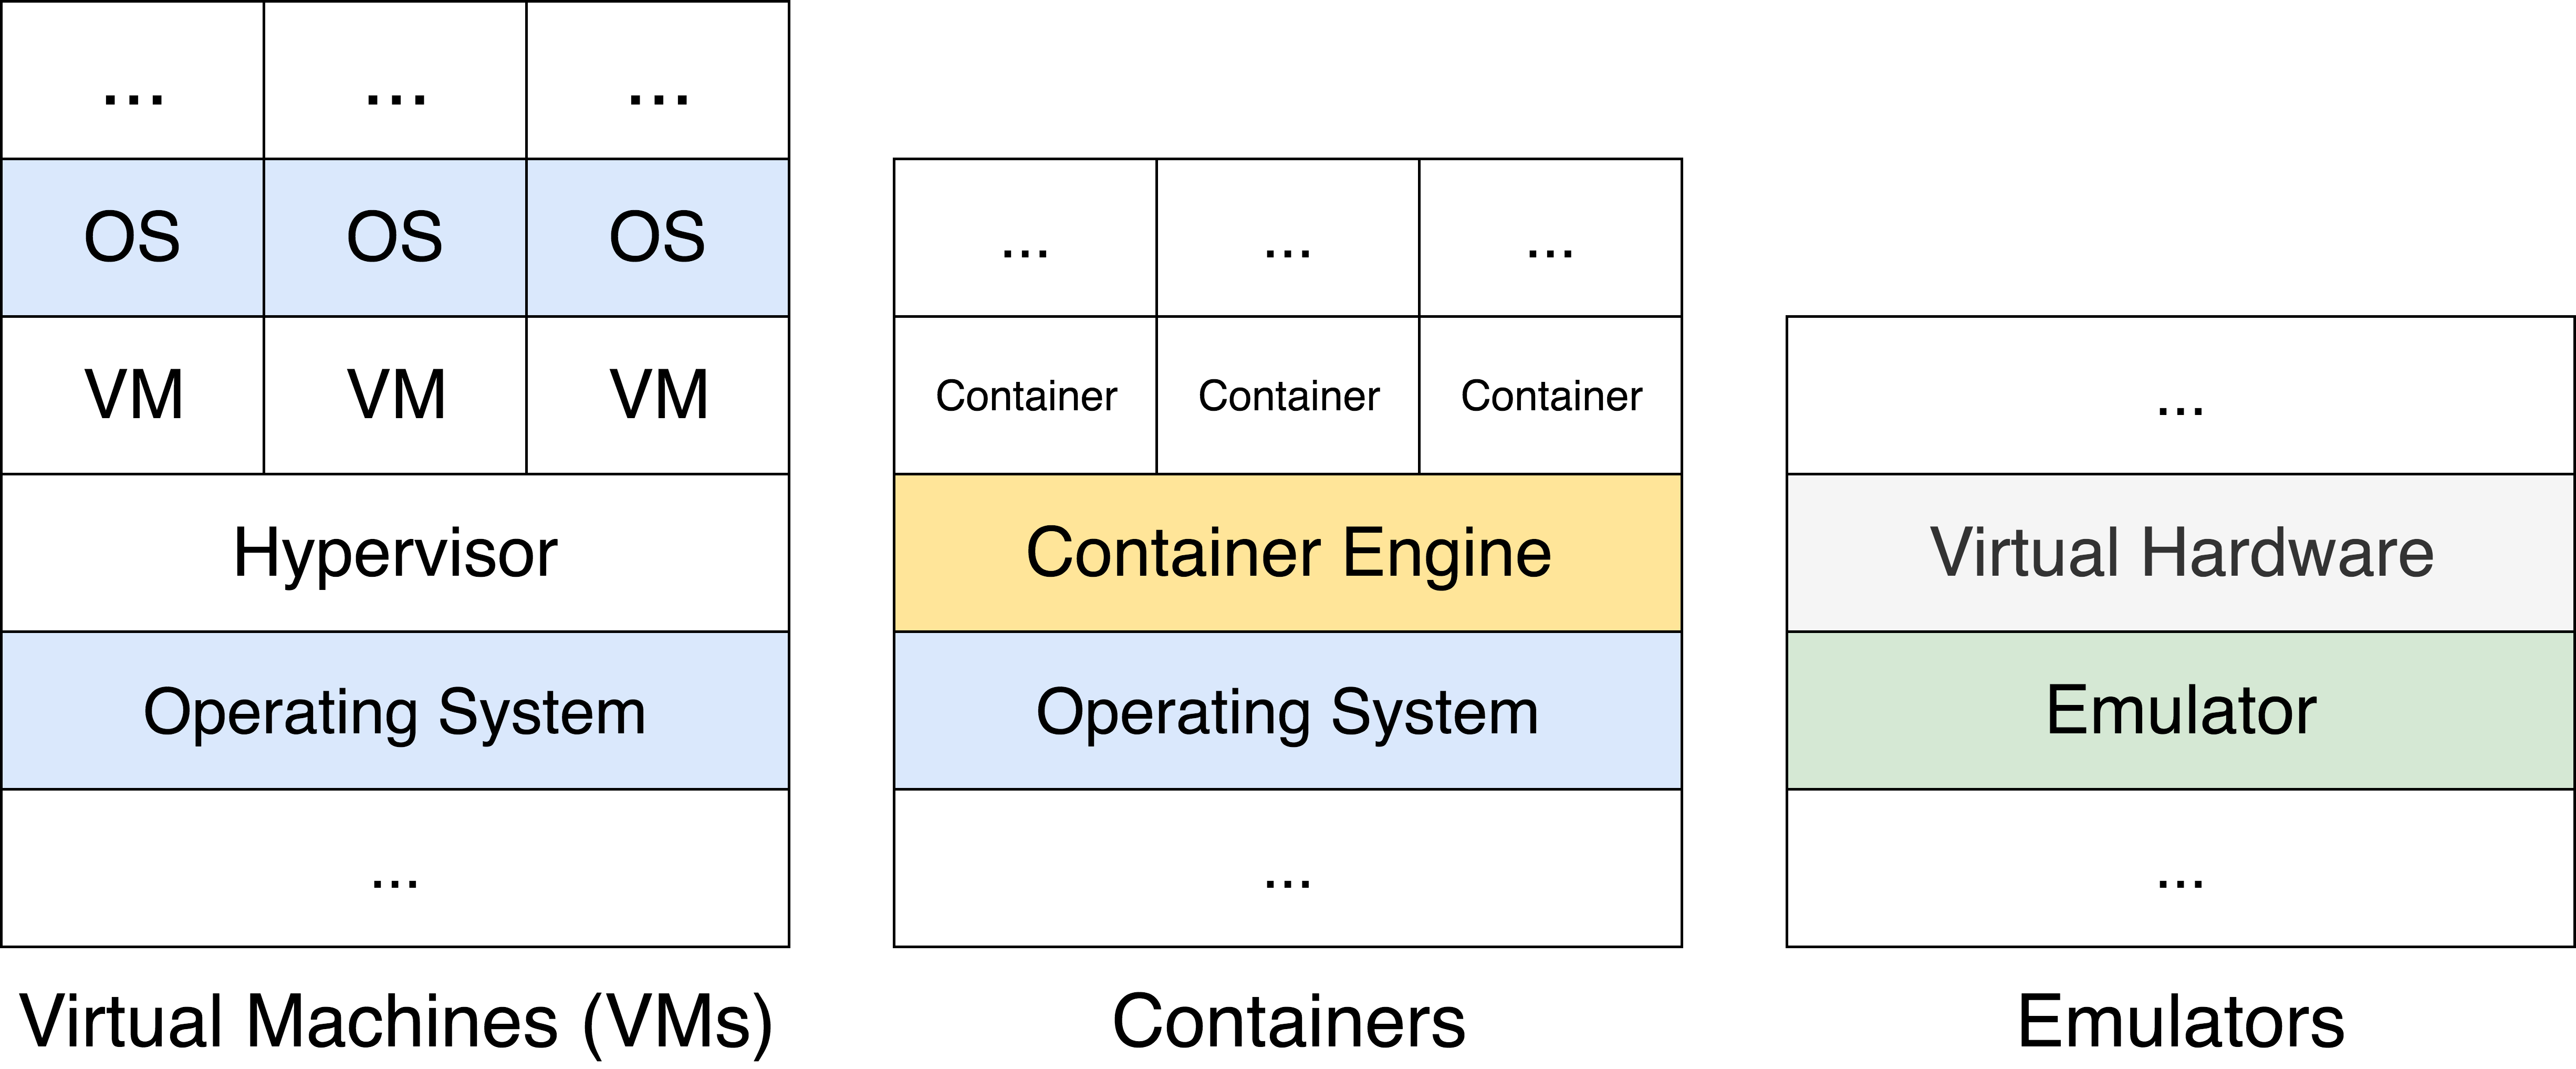
\includegraphics[width=0.70\textwidth]{../figures/vms_containers_emulators.png}
\caption{La virtualisation complète est un processus très gourmand en ressources. La conteneurisation est moins coûteuse, car elle partage un noyau avec le système d'exploitation hôte. L'émulation nous permet d'émuler le matériel comme un logiciel. Chacune de ces méthodes peut être utilisée en conjonction avec n'importe quelle autre.\vspace{-10pt}}
\label{fig:vms_containers_emulators}
\end{figure}

\section{Containerization}\label{sec:containerization}

L'un des défis du développement de logiciels distribués sur des plates-formes hétérogènes est le problème de la variabilité. L'accélération du rythme de développement des logiciels s'accompagne d'une charge supplémentaire de maintenance des logiciels. À mesure que les piles de matériel et de logiciels évoluent, le code source doit être périodiquement mis à jour pour être construit et fonctionner correctement. Maintenir une base de code stable et bien documentée peut représenter un défi considérable, en particulier dans un cadre universitaire où les contributeurs rejoignent et quittent fréquemment un projet. Ensemble, ces défis constituent des obstacles importants à la reproductibilité expérimentale et à la collaboration scientifique.

\begin{figure}[ht]
\centrer
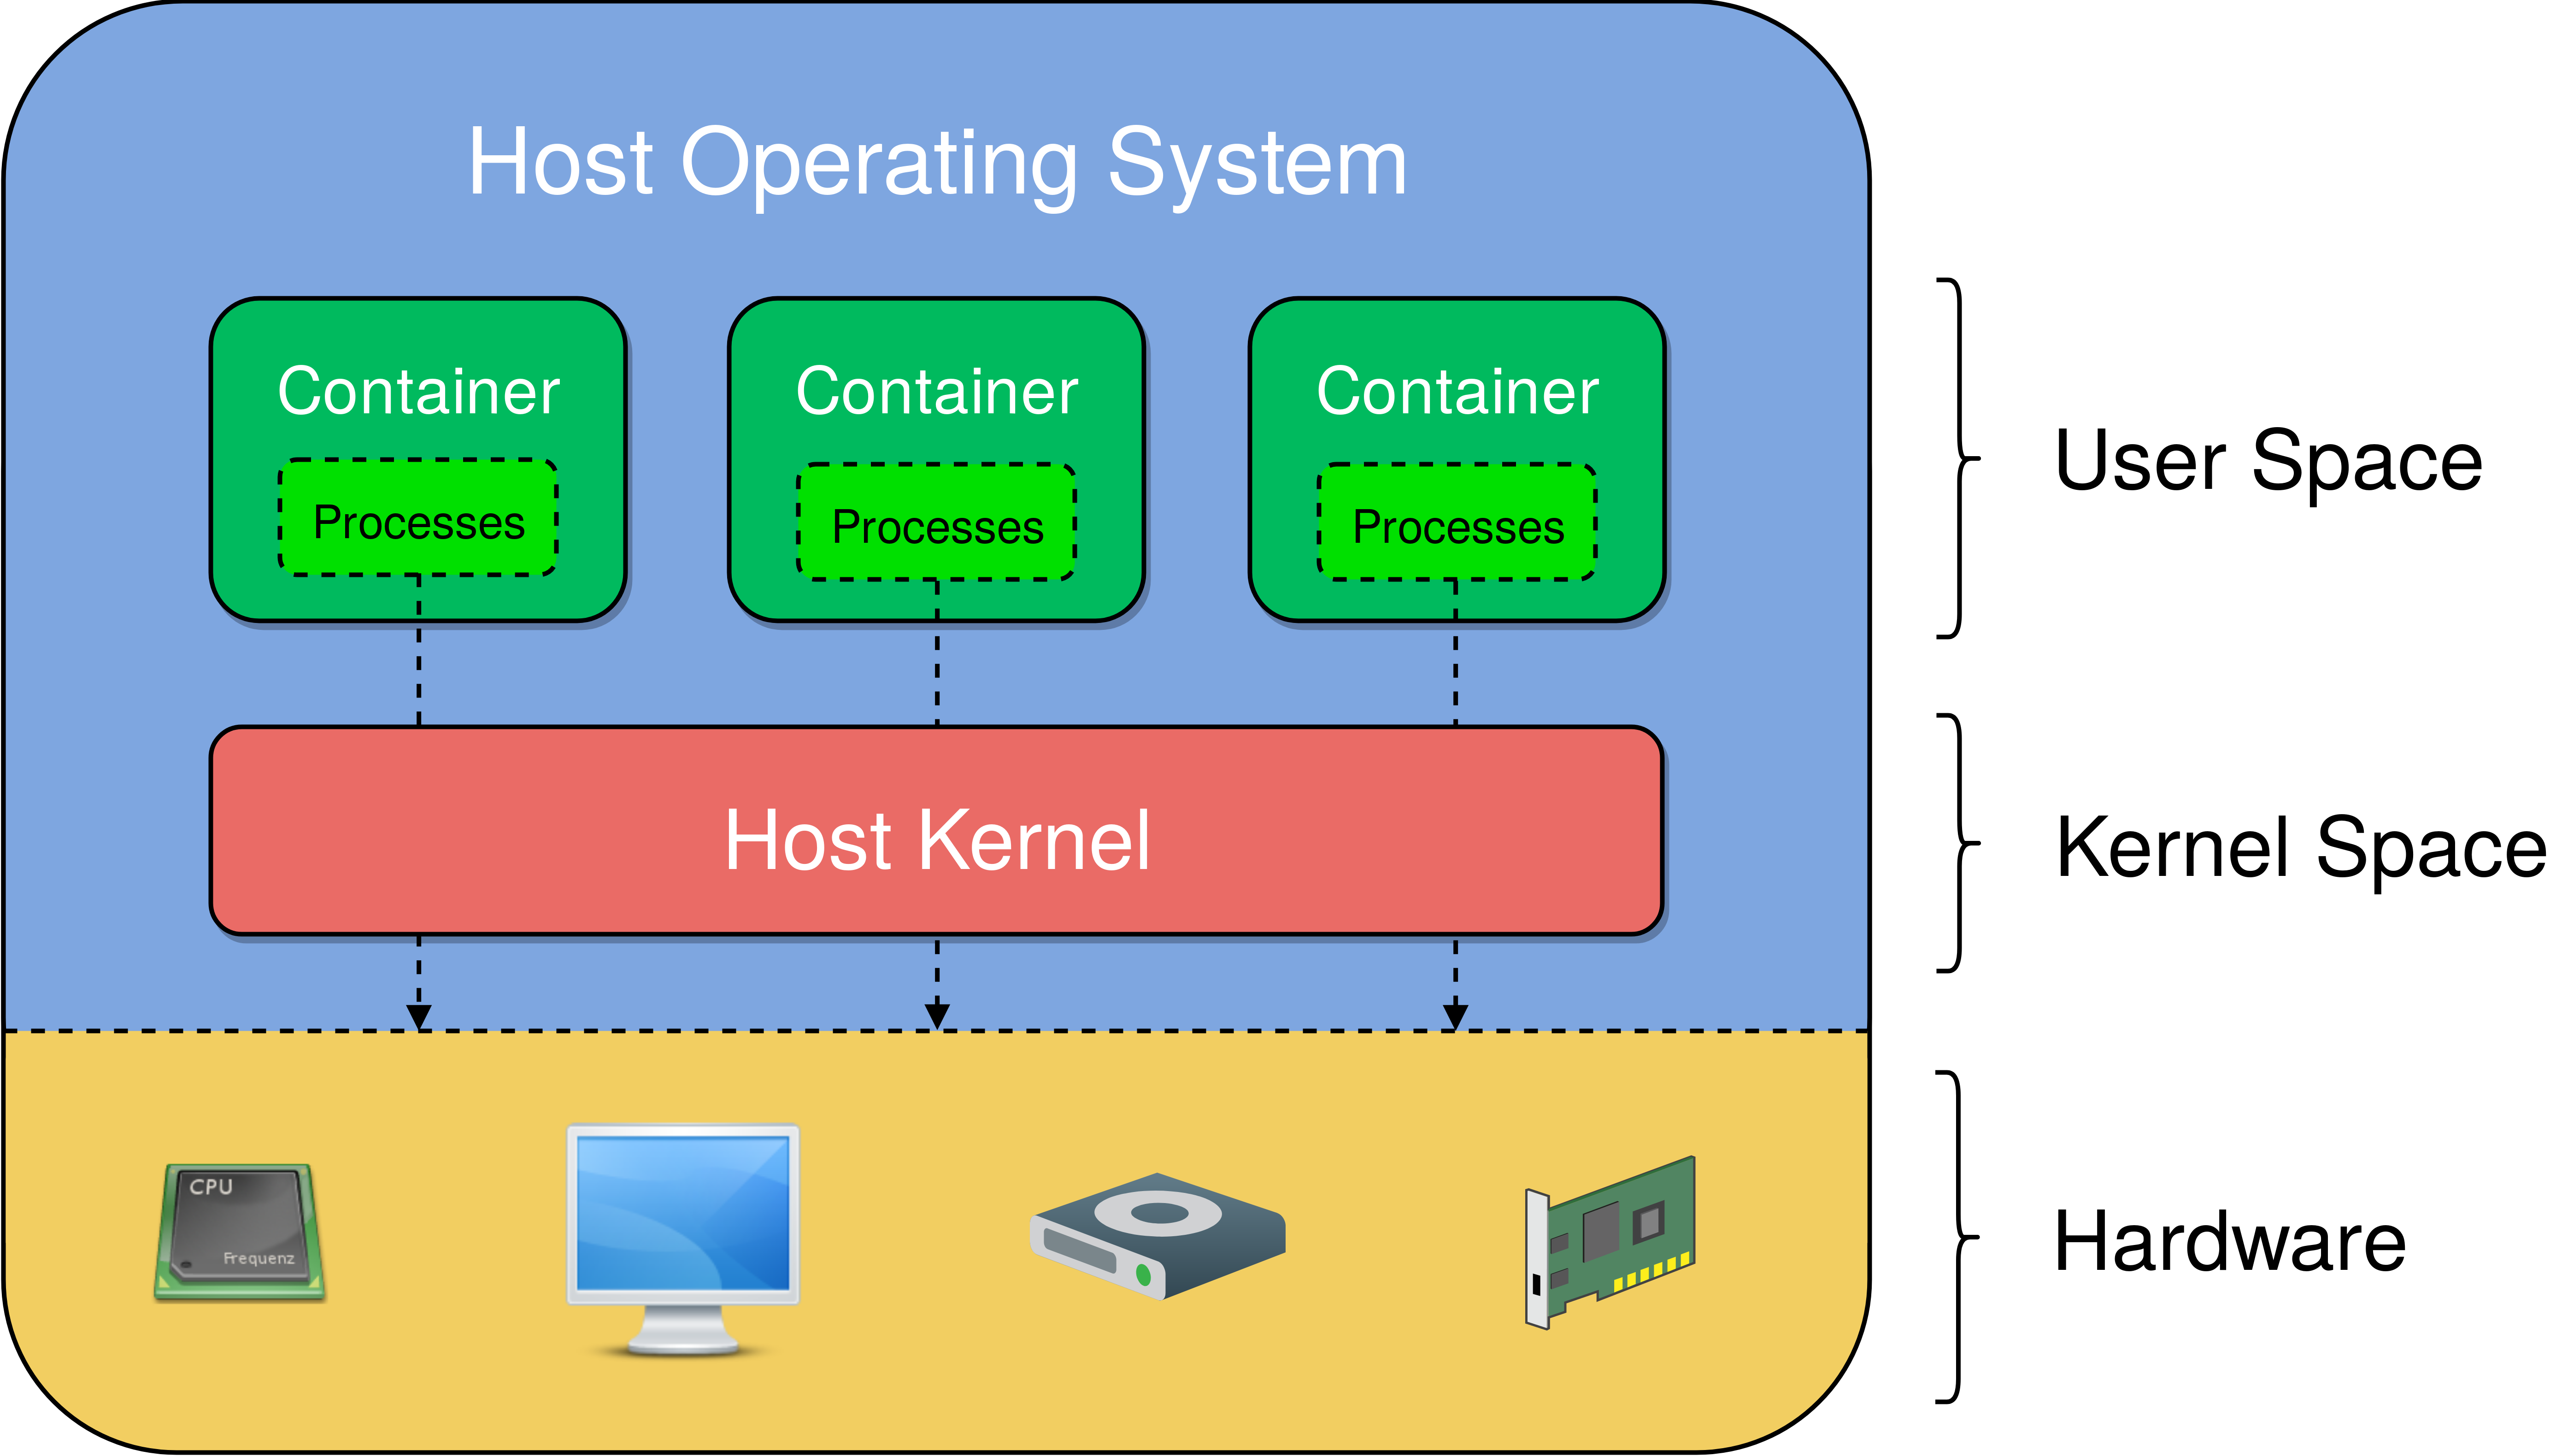
\includegraphics[width=0.65\textwidth]{../figures/user_kernel_hardware.png}
\caption{Containers live in user space. Par défaut, ils sont mis en bac à sable à partir de l'OS hôte et des conteneurs frères et sœurs, mais contrairement aux VM, ils partagent un noyau commun entre eux et avec l'OS hôte. Tous les appels système sont passés par le noyau hôte.}
\label{fig:user_kernel_hardware}
\end{figure}

Les conteneurs Docker sont des environnements d'exécution en bac à sable qui sont portables, reproductibles et dont la version est contrôlée. Chaque environnement contient toutes ses dépendances, mais reste isolé du système d'exploitation et du système de fichiers hôte. Docker fournit un mécanisme pour contrôler les ressources auxquelles chaque conteneur est autorisé à accéder, et fournit un espace de noms Linux séparé pour chaque conteneur, isolant efficacement le réseau, les utilisateurs et les montages du système de fichiers du système d'exploitation hôte. Contrairement aux machines virtuelles, les outils de virtualisation basés sur des conteneurs comme Docker sont adaptés aux SBC portables et peuvent fonctionner avec une surcharge proche de zéro par rapport aux processus Linux natifs. Un seul Raspberry Pi est capable d'exécuter simultanément des centaines de conteneurs sans dégradation notable des performances. Espace{-.08em}\footnote{\url{https://blog.docker.com/2015/09/update-raspberry-pi-dockercon-challenge/}}

Si la conteneurisation simplifie considérablement le processus de création et de déploiement des applications, elle introduit également une certaine complexité supplémentaire dans le cycle de vie du développement des logiciels. Docker, comme la plupart des plates-formes de conteneur, utilise un système de fichiers en couches. Cela permet à Docker de prendre une "image" existante et de la modifier en installant de nouvelles dépendances ou en modifiant ses fonctionnalités. Les images sont généralement construites comme une séquence de couches, chacune devant être mise à jour périodiquement. Il faut veiller, lors de la conception du pipeline de développement, à ce que ces mises à jour ne brisent pas silencieusement une couche suivante, comme nous le décrivons dans \autoref{sec:retrospective}.

\section{Introduction to Docker}\label{sec:docker-intro}

Supposons qu'il existe un programme connu pour fonctionner sur un ordinateur quelconque. Il serait bon de donner à un autre ordinateur -- n'importe quel ordinateur connecté à Internet -- une courte chaîne de caractères ASCII, d'appuyer sur les touches \keys{\return}, et de revenir pour voir ce même programme s'exécuter. Peu importe où le programme a été construit ou quel logiciel était en cours d'exécution à ce moment-là. Cela peut sembler trivial, mais c'est un problème monumental de génie logiciel. Divers gestionnaires de paquets ont tenté de résoudre ce problème, mais même lorsqu'ils fonctionnent comme prévu, ils ne prennent en charge que les binaires compilés en natif sur les systèmes d'exploitation ayant le même gestionnaire de paquets.

Docker\footnote{Le tutoriel suivant utilise Docker, mais le flux de travail décrit est similaire à celui de la plupart des plateformes de conteneurs.} est un outil de calcul portable et reproductible. Avec Docker, les utilisateurs peuvent exécuter n'importe quel programme Linux sur presque tous les appareils informatiques en réseau de la planète, quel que soit le système d'exploitation ou l'architecture matérielle sous-jacents. Toutes les étapes de préparation, d'installation et de configuration de l'environnement peuvent être automatisées du début à la fin. Selon la largeur de bande disponible sur le réseau, cela peut prendre un certain temps, mais les utilisateurs n'auront jamais besoin d'intervenir dans le processus d'installation.

Pour installer Docker lui-même, exécutez la commande suivante sur un shell conforme à POSIX de n'importe quelle \href{https://docs.docker.com/install/#supported-platforms}{Plateforme supportée par Docker}:

\begin{pclisting}
    ~$ curl -sSL https://get.docker.com/ | sh
\end{pclisting}
%
Un Docker \textit{image} est essentiellement un instantané du système de fichiers -- un fichier unique qui contient tout ce qui est nécessaire pour faire fonctionner un certain conteneur du Docker. Les images des Dockers sont hébergées dans des \textit{registres}, similaires aux dépôts Git ou aux serveurs VCS. La commande suivante permet d'extraire une image Docker, par exemple \inline{daphne/duck} du dépôt par défaut \hyperref[subsec:docker_hub]{Docker Hub}:

\begin{pclisting}
    ~$ docker pull (*@\hl{daphne/duck}@*)
\end{pclisting}
%
Chaque image du Docker a un identifiant, un nom et une étiquette:

\begin{pclisting}
~$ docker images
REPOSITORY      TAG        IMAGE ID         CREATED       SIZE
(*@\hl{daphne/duck}@*)     latest     ea2f90g8de9e     1 day ago     869MB
\end{pclisting}
%
Pour lancer un conteneur Docker, utilisez la commande suivante:

\begin{pclisting}
~$ docker run daphne/duck
\end{pclisting}
%
La commande suivante permet de vérifier que le conteneur est bien en cours d'exécution:

\begin{pclisting}
~$ docker ps
CONTAINER ID     IMAGE           ...     NAMES
52994ef22481     daphne/duck     ...     (*@\hl{happy\_hamster}@*)
\end{pclisting}
%
Notez que l'image de Daphné possède un identifiant alphanumérique du conteneur, \inline{52994ef22481}, une image de base, \inline{daphne/duck}, et un nom mémorable, \inline{happy\_hamster}. Ce nom est un alias pour l'ID du conteneur, qui peut être utilisé de manière interchangeable pour faire référence au conteneur.

Les images de docker peuvent être créées de deux manières différentes. Tout d'abord, dans \autoref{subsec:creating-an-image-snapshot}, nous verrons comment créer une image Docker en prenant un instantané d'un conteneur en cours d'exécution, puis dans \autoref{subsec:writing-an-image-recipe}, comment créer un nouveau conteneur Docker en utilisant un type de recette spécial, appelé \href{https://docs.docker.com/engine/reference/builder/}{\inline{Dockerfile}}.

\subsection{Creating an image snapshot}\label{subsec:creating-an-image-snapshot}}, comment créer un nouveau conteneur Docker en utilisant une recette spéciale, appelée \href{}{\inline{Dockerfile}}.

Lorsqu'un conteneur du Docker écrit sur son propre système de fichiers, ces modifications ne sont pas persistantes, sauf si elles sont appliquées à une nouvelle image. Par exemple, démarrez un conteneur avec un shell interactif:

\begin{pclisting}
~$ docker run -it daphne/duck /bin/bash
root@(*@\hl{295fd7879184}@*):/#
\end{pclisting}
%
Notez l'ID du conteneur : \inline{295fd7879184}. Si on écrit sur le disque et qu'on laisse le conteneur,

\begin{pclisting}
root@295fd7879184:/# touch (*@\hl{new\_file}@*) && ls -l
total 0
-rw-r--r-- 1 root root 0 May 21 20:52 (*@\hl{new\_file}@*)
root@295fd7879184:/# exit
\end{pclisting}
%
\inline{new\_file} ne sera pas persisté. Si nous relançons la même commande:

\begin{pclisting}
~$ docker run -it daphne/duck /bin/bash
root@18f13bb4571a:/# ls
root@18f13bb4571a:/# touch new_file1 && ls -l
total 0
-rw-r--r-- 1 root root 0 May 21 21:32 new_file1
\end{pclisting}
%
Il semble que le "nouveau fichier" ait disparu ! Remarquez que l'ID du conteneur (\inline{18f13bb4571a}) est maintenant différent. C'est parce que la commande \inline{docker run daphne/duck} a créé un nouveau conteneur à partir de l'image de base \inline{daphne/duck}, plutôt que de redémarrer le conteneur précédent. Pour voir tous les conteneurs sur un hôte Docker, exécutez la commande suivante:

\begin{pclisting}
~$ docker container ls -a
CONTAINER ID      IMAGE            STATUS             NAMES
295fd7879184      daphne/duck      Exited (130)       merry_manatee
18f13bb4571a      daphne/duck      Up 5 minutes       shady_giraffe
52994ef22481      daphne/duck      Up 10 minutes      happy_hamster
\end{pclisting}
%
Il semble que \inline{295fd7879184} alias \inline{merry\_manatee} ait survécu, mais il ne fonctionne plus. Chaque fois que le processus principal d'un conteneur (rappelons que nous avons exécuté \inline{merry\_manatee} avec \inline{/bin/bash}) se termine, le conteneur s'arrête, mais il ne cesse pas d'exister. En fait, nous pouvons reprendre le conteneur arrêté là où il s'est arrêté:
%
\begin{pclisting}
~$ docker start -a merry_manatee
root@295fd7879184:/# ls -l
total 0
-rw-r--r-- 1 root root 0 May 21 20:52 new_file
\end{pclisting}
%
Rien n'a été perdu ! Pour le vérifier, nous pouvons vérifier quels autres conteneurs sont en cours d'utilisation:

\begin{pclisting}
~$ docker ps
CONTAINER ID       IMAGE             ...       NAMES
295fd7879184       daphne/duck       ...       merry_manatee
18f13bb4571a       daphne/duck       ...       shady_giraffe
52994ef22481       daphne/duck       ...       happy_hamster
\end{pclisting}
%
Supposons maintenant que nous voulions partager le conteneur \inline{shady\_giraffe} avec quelqu'un d'autre. Pour ce faire, nous devons d'abord prendre un instantané du conteneur en cours d'utilisation, ou le placer dans une nouvelle image avec un nom et une balise. Cela créera un point de contrôle que nous pourrons restaurer ultérieurement:

\begin{pclisting}
~$ docker commit -m "forking daphne/duck" (*@\hl{shady\_giraffe}@*) user/duck:v2
\end{pclisting}
%
Pour faire référence au conteneur, on peut utiliser soit \inline{18f13bb4571a} soit le nom désigné, c'est-à-dire \inline{shady\_giraffe}. Ce dépôt d'images sera appelé \inline{user/duck}, et possède un identifiant de version optionnel, \inline{:v2}, qui peut être poussé dans le registre \hyperref[subsec:docker_hub]{Docker Hub}:

\begin{pclisting}
~$ docker push (*@\hl{user/duck:v2}@*)
~$ docker images
REPOSITORY    TAG        IMAGE ID         CREATED          SIZE
daphne/duck   latest     ea2f90g8de9e     1 day ago        869MB
user/duck     v2         d78be5cf073e     2 seconds ago    869MB
~$ docker pull user/duck:v2
~$ docker run user/duck:v2 ls -l
total 0
-rw-r--r-- 1 root root 0 May 21 21:32 new_file1
\end{pclisting}
%
C'est un moyen pratique de partager une image avec des collègues et des collaborateurs. Toute personne ayant accès au dépôt peut retirer cette image et continuer là où nous nous sommes arrêtés, ou créer une autre image basée sur le dessus.

\subsection{Writing an image recipe}\label{subsec:writing-an-image-recipe}

La deuxième façon de créer une image Docker est d'écrire une recette, appelée \inline{Dockerfile}. Un \inline{Dockerfile} est un fichier texte qui spécifie les commandes requises pour créer une image du Docker, généralement en modifiant une image de conteneur existante à l'aide d'une interface de script. Ils comportent également des \href{https://docs.docker.com/engine/reference/builder/}{mots-clés} spéciaux (qui sont traditionnellement \inline{CAPITALIZED}), comme \href{https://docs.docker.com/engine/reference/builder/#from}{\inline{FROM}}, \href{https://docs.docker.com/engine/reference/builder/#from}{\inline{RUN}}, \href{https://docs.docker.com/engine/reference/builder/#entrypoint}{\inline{ENTRYPOINT}} et ainsi de suite. Par exemple, créez un fichier appelé \inline{Dockerfile}} avec le contenu suivant:

\begin{dockerlisting}
FROM daphne/duck      # Defines the base image
RUN touch new_file1   # new_file1 will be part of our snapshot
CMD ls -l             # Default command run when container is started
\end{dockerlisting}
%
Maintenant, pour construire l'image, nous pouvons simplement courir:

\begin{pclisting}
~$ docker build -t user/duck:v3 (*@\hl{.}@*)
\end{pclisting}
%
Le \inline{.} indique le répertoire courant, qui doit être le même que celui contenant notre \inline{Dockerfile}. Cette commande devrait produire quelque chose comme la sortie suivante:

\begin{pclisting}
Sending build context to Docker daemon  2.048kB
Step 1/3 : FROM daphne/duck
--- ea2f90g8de9e
Step 2/3 : RUN touch new_file1
--- e3b75gt9zyc4
Step 3/3 : CMD ls -l
--- Running in 14f834yud59
Removing intermediate container 14f834yud59
--- 05a3bd381fc2
Successfully built 05a3bd381fc2
Successfully tagged user/duck:v3
\end{pclisting}
%
La commande, \inline{docker images} devrait afficher une image appelée \inline{user/duck:v3}:

\begin{pclisting}
~$ docker images
REPOSITORY    TAG        IMAGE ID         CREATED          SIZE
daphne/duck   latest     ea2f90g8de9e     1 day ago        869MB
user/duck     v2         d78be5cf073e     5 minutes ago    869MB
user/duck     v3         05a3bd381fc2     2 seconds ago    869MB
\end{pclisting}
%
Cette procédure est identique à la technique d'instantané réalisée dans \autoref{subsec:creating-an-image-snapshot}, mais le résultat est plus propre. Plutôt que de conserver une image de 869 Mo, on peut se contenter de stocker le fichier texte de 4 Ko. Pour exécuter l'image résultante, nous pouvons simplement utiliser la même commande qu'auparavant:

\begin{pclisting}
~$ docker run -it (*@\hl{user/duck:v3}@*)
total 0
-rw-r--r-- 1 root root 0 May 21 21:35 new_file1
\end{pclisting}
%
Notez que dès que nous lançons le conteneur, Docker exécute la commande \inline{ls -l} comme spécifié par le \inline{Dockerfile}, révélant que \inline{new\_file1} a bien été stocké dans l'image. Cependant, cette commande par défaut peut être remplacée par une commande personnalisée:

\begin{pclisting}
~$ docker run -it user/duck:v3 (*@\hl{[custom command]}@*)
\end{pclisting}
%
\subsection{Layer caching}

\href{https://docs.docker.com/storage/storagedriver/#images-and-layers}{Layers} sont un concept important à comprendre quand on travaille avec Docker. Une façon de penser à une couche est comme un commit Git -- un ensemble de modifications à une image ou une couche précédente, identifiée de façon unique par un code de hachage. Dans un \inline{Dockerfile}, les calques commencent par un \href{https://docs.docker.com/engine/reference/builder/#from}{mot-clé}.

\begin{dockerlisting}
FROM daphne/duck
RUN touch new_file1                            # Defines a new layer
RUN mkdir config && mv new_file1 config        # Layers can chain commands
RUN apt-get update && apt-get install -y wget  # Install a dependency
RUN wget https://get.your.app/install.sh       # Download a script
RUN chmod +x install.sh && ./install.sh        # Run the script
\end{dockerlisting}
%
Pour construire cette image, nous pouvons exécuter la commande suivante:

\begin{pclisting}
~$ docker build -t user/duck:v4 .
Sending build context to Docker daemon  2.048kB
Step 1/6 : FROM daphne/duck
---> cd6d8154f1e1
...
Removing intermediate container 8fb56ef38bc8
---> 3358ca1b8649
Step 5/6 : RUN wget https://get.your.app/install.sh
---> Running in e8284ff4ec8b
...
2018-10-30 06:47:57 (89.9 MB/s) - 'install.sh' saved [13847/13847]
Removing intermediate container e8284ff4ec8b
---> 24a22dc2900a
Step 6/6 : RUN chmod +x install.sh && ./install.sh
---> Running in 9526651fa492
# Executing install script, commit: 36b78b2
...
Removing intermediate container 9526651fa492
---> a8be23fea573
Successfully built a8be23fea573
Successfully tagged user/duck:v4
\end{pclisting}
%
Les couches sont mises en cache de manière pratique par le \href{https://docs.docker.com/engine/reference/commandline/dockerd/}{Docker daemon}. Si nous devons exécuter deux fois la même commande, Docker utilisera le cache au lieu de reconstruire l'image entière:

\begin{pclisting}
Sending build context to Docker daemon  2.048kB
Step 1/6 : FROM daphne/duck
---> cd6d8154f1e1
Step 2/6 : RUN touch new_file1
---> (*@\hl{Using cache}@*)
---> 0473154b2004
...
Step 6/6 : RUN chmod +x index.html && ./index.html
---> (*@\hl{Using cache}@*)
---> a8be23fea573
Successfully built a8be23fea573
Successfully tagged user/duck:v4
\end{pclisting}
%
Si nous devons apporter une modification au \inline{Dockerfile}, Docker ne reconstruira l'image qu'à partir de la première étape modifiée. Supposons que nous ajoutions une nouvelle commande \inline{RUN} à la fin de notre \inline{Dockerfile} et que nous déclenchions une reconstruction de la même manière:

\begin{pclisting}
~$ echo 'RUN echo "(*@\hl{Change here!}@*)"' >> Dockerfile
~$ docker build -t user/duck:v4 .
Sending build context to Docker daemon  2.048kB
...
Step 6/7 : RUN chmod +x index.html && ./index.html
---> Using cache
---> a8be23fea573
Step 7/7 : RUN echo "Change here!"
---> Running in 80fc5c402304
(*@\hl{Change here!}@*)
Removing intermediate container 80fc5c402304
---> c1ec64cef9c6
Successfully built c1ec64cef9c6
Successfully tagged user/duck:v4
\end{pclisting}
%
Si Docker devait relancer l'ensemble du [fichier] en ligne de haut en bas à chaque reconstruction, cela serait lent et peu pratique. Au lieu de cela, Docker met en cache les étapes non modifiées par défaut, et ne refait que le minimum d'étapes nécessaires à la reconstruction. Cela peut parfois donner des résultats inattendus, surtout lorsque la cache est périmée. Pour ignorer le cache et forcer une reconstruction propre, utilisez l'indicateur \inline{-{}-no-cache} lors de la construction d'un \inline{Dockerfile}.

Que prend en compte Docker pour décider d'utiliser le cache? Tout d'abord, le \inline{Dockerfile} lui-même - lorsqu'une étape d'un \inline{Dockerfile} change, elle et toutes les étapes suivantes devront être relancées lors de la compilation. Docker vérifie également le \href{https://docs.docker.com/engine/reference/commandline/build/#extended-description}{contexte de construction} pour les changements. Lorsque \inline{docker build -t TAG .} est écrit, le \inline{.} indique le contexte de construction, ou le chemin où la construction doit avoir lieu. Souvent, ce chemin contient des artefacts de compilation. Par exemple:

\begin{dockerlisting}
FROM daphne/duck
COPY duck.txt .
RUN cat duck.txt
\end{dockerlisting}
%
Maintenant, si nous ajoutons un message dans \inline{duck.txt} et reconstruisons notre image, le fichier sera copié dans l'image du Docker, et son contenu sera imprimé:

\begin{pclisting}
~$ echo "(*@\hl{Make way!}@*)" > duck.txt && docker build -t user/duck:v5 .
Sending build context to Docker daemon  3.072kB
Step 1/3 : FROM daphne/duck
---> cd6d8154f1e1
Step 2/3 : COPY duck.txt .
---> e0e03d9e1791
Step 3/3 : RUN cat duck.txt
---> Running in 590c5420ce29
(*@\hl{Make way!}@*)
Removing intermediate container 590c5420ce29
---> 1633e3e10bef
Successfully built 1633e3e10bef
Successfully tagged user/duck:v5
\end{pclisting}
%
Tant que les trois premières lignes du \inline{Dockerfile} et du \inline{duck.txt} ne sont pas modifiées, ces couches seront mises en cache et Docker ne les reconstruira pas. Si le contenu du fichier \inline{duck.txt} est modifié par la suite, cela déclenchera une reconstruction. Par exemple, si nous ajoutons au fichier et le reconstruisons, seules les deux dernières étapes devront être exécutées:

\begin{pclisting}
~$ echo "(*@\hl{Thank you. Have a nice day!}@*)" >> duck.txt
~$ docker build -t user/duck:v5 .
Sending build context to Docker daemon  3.072kB
Step 1/3 : FROM ubuntu
---> cd6d8154f1e1
Step 2/3 : COPY duck.txt .
---> f219efc150a5
Step 3/3 : RUN cat duck.txt
---> Running in 7c6f5f8b73e9
(*@\hl{Make way!}@*)
(*@\hl{Thank you. Have a nice day!}@*)
Removing intermediate container 7c6f5f8b73e9
---> e8a1db712aee
Successfully built e8a1db712aee
Successfully tagged user/duck:v5
\end{pclisting}
%
Une erreur courante lors de l'écriture de \inline{Dockerfile}s consiste à \inline{COPY} plus de fichiers que ce qui est strictement nécessaire pour effectuer l'étape de construction suivante. Par exemple, si \inline{COPY . .} est écrit au début du \inline{Dockerfile}, chaque fois qu'un fichier est modifié dans le contexte de la compilation, cela déclenchera une reconstruction de toutes les étapes de compilation suivantes. Afin de maximiser la réutilisation du cache et de réduire au minimum le temps de reconstruction, les utilisateurs doivent être aussi prudents que possible et ne \inline{COPY} que le minimum de fichiers nécessaires pour accomplir l'étape de construction suivante.

% Comme le \inline{.gitignore} de Git, Docker a également un fichier \inline{.dockerignore}. Si nous ajoutons une ligne au fichier \inline{.dockerignore}, alors tous les chemins correspondant à cette ligne dans le contexte de compilation seront ignorés. Docker accepte également d'autres motifs comme les expressions régulières et la négation.~\footnote{Further details : \url{https://docs.docker.com/engine/reference/builder/#dockerignore-file}}

\subsection{Volume sharing}\label{subsec:volume_sharing}

Il existe une deuxième méthode pour déposer les données dans un conteneur, qui ne nécessite pas de les intégrer dans l'image mère au moment de la compilation. Cette méthode est plus appropriée pour les données qui sont nécessaires au moment de l'exécution, mais non essentielles pour la construction. Elle prend la forme suivante:

\begin{pclisting}
~$ docker run user/duck:v6 (*@\hl{-v HOST\_PATH:TARGET\_PATH}@*)
\end{pclisting}
%
Supposons que nous ayons un \inline{Dockerfile} qui fournit une instruction \inline{CMD} par défaut:

\begin{dockerlisting}
de daphne/duck
CMD /bin/bash -c "/launch.sh"
\end{dockerlisting}
%
Si nous construisions cette image et essayions de l'exécuter, le fichier \inline{/launch.sh} serait manquant:

\begin{pclisting}
~$ docker build -t user/duck:v6 && docker run user/duck:v6
bash: (*@\hl{/launch.sh}@*): No such file or directory
\end{pclisting}
%
Au lieu de cela, lorsque nous utilisons le conteneur, nous devons partager le fichier via le Docker CLI:

\begin{pclisting}
~$ echo -e '#!/bin/bash\necho Launching...' >> launch.sh && \
   chmod 775 launch.sh && \
   docker run user/duck:v6 (*@\hl{-v launch.sh:/launch.sh}@*)
Launching...
\end{pclisting}
%
De cette façon, le fichier local \inline{launch.sh} sera disponible pour être utilisé à l'intérieur du conteneur au chemin désigné, \inline{/launch.sh}.

\subsection{Multi-stage builds}

Le système de fichiers de Docker est additif, donc chaque couche ne fera qu'augmenter la taille de l'image finale. Pour cette raison, il est souvent nécessaire de mettre de l'ordre dans les fichiers inutiles après l'installation. Par exemple, lors de l'installation de dépendances sur des images basées sur Debian, il est courant de les exécuter:

\begin{dockerlisting}
RUN apt-get update && apt-get install ... && (*@\hl{rm -rf /var/lib/apt/lists/*}@*)
\end{dockerlisting}
%
Cela garantit que la liste des paquets n'est pas intégrée à l'image (Docker ne vérifie le calque qu'une fois chaque étape terminée). Les constructions peuvent souvent consommer plusieurs étapes, bien qu'elles ne produisent qu'un seul artefact. Au lieu d'enchaîner plusieurs commandes et de nettoyer les changements en une seule étape, les constructions à plusieurs étapes nous permettent de construire une série d'images à l'intérieur d'un \inline{Dockerfile}, et de copier les ressources de l'une à l'autre, en éliminant tous les artefacts de construction intermédiaires:

\begin{dockerlisting}
FROM user/duck:v3 as template1

FROM daphne/duck as template2
COPY --from=template1 new_file1 new_file2
FROM donald/duck as template3
COPY --from=template2 new_file2 (*@\hl{new\_file3}@*)
CMD ls -l
\end{dockerlisting}
%
Nous pouvons maintenant construire et faire fonctionner cette image comme suit:

\begin{pclisting}
~$ docker build . -t user/duck:v4
Sending build context to Docker daemon  2.048kB
Step 1/6 : FROM user/duck:v3 as template1
--- e3b75ef8ecc4
Step 2/6 : FROM daphne/duck as template2
--- ea2f90g8de9e
Step 3/6 : COPY --from=template1 new_file1 new_file2
---> 72b96668378e
Step 4/6 : FROM donald/duck:v3 as template3
---> e3b75ef8ecc4
Step 5/6 : COPY --from=template2 new_file2 (*@\hl{new\_file3}@*)
---> cb1b84277228
Step 6/6 : CMD ls
---> Running in cb1b84277228
Removing intermediate container cb1b84277228
---> c7dc5dd63e77
Successfully built c7dc5dd63e77
Successfully tagged user/duck:v4
~$ docker run -it user/duck:v4
total 0
-rw-r--r-- 1 root root 0 Jul  8 15:06 (*@\hl{new\_file3}@*)
\end{pclisting}
%
Une des applications des constructions en plusieurs étapes consiste à compiler une dépendance de projet à partir de son code source. En plus de tout le code source, le processus de compilation pourrait introduire des gigaoctets d'artefacts de construction et de dépendances transitives, juste pour construire un seul binaire. Les compilations multi-étapes nous permettent de construire le fichier, et de le copier sur une nouvelle couche, libérée des fichiers intermédiaires.

\section{ROS and Docker}\label{sec:ros-docker}

\begin{figure}[ht]
\centering
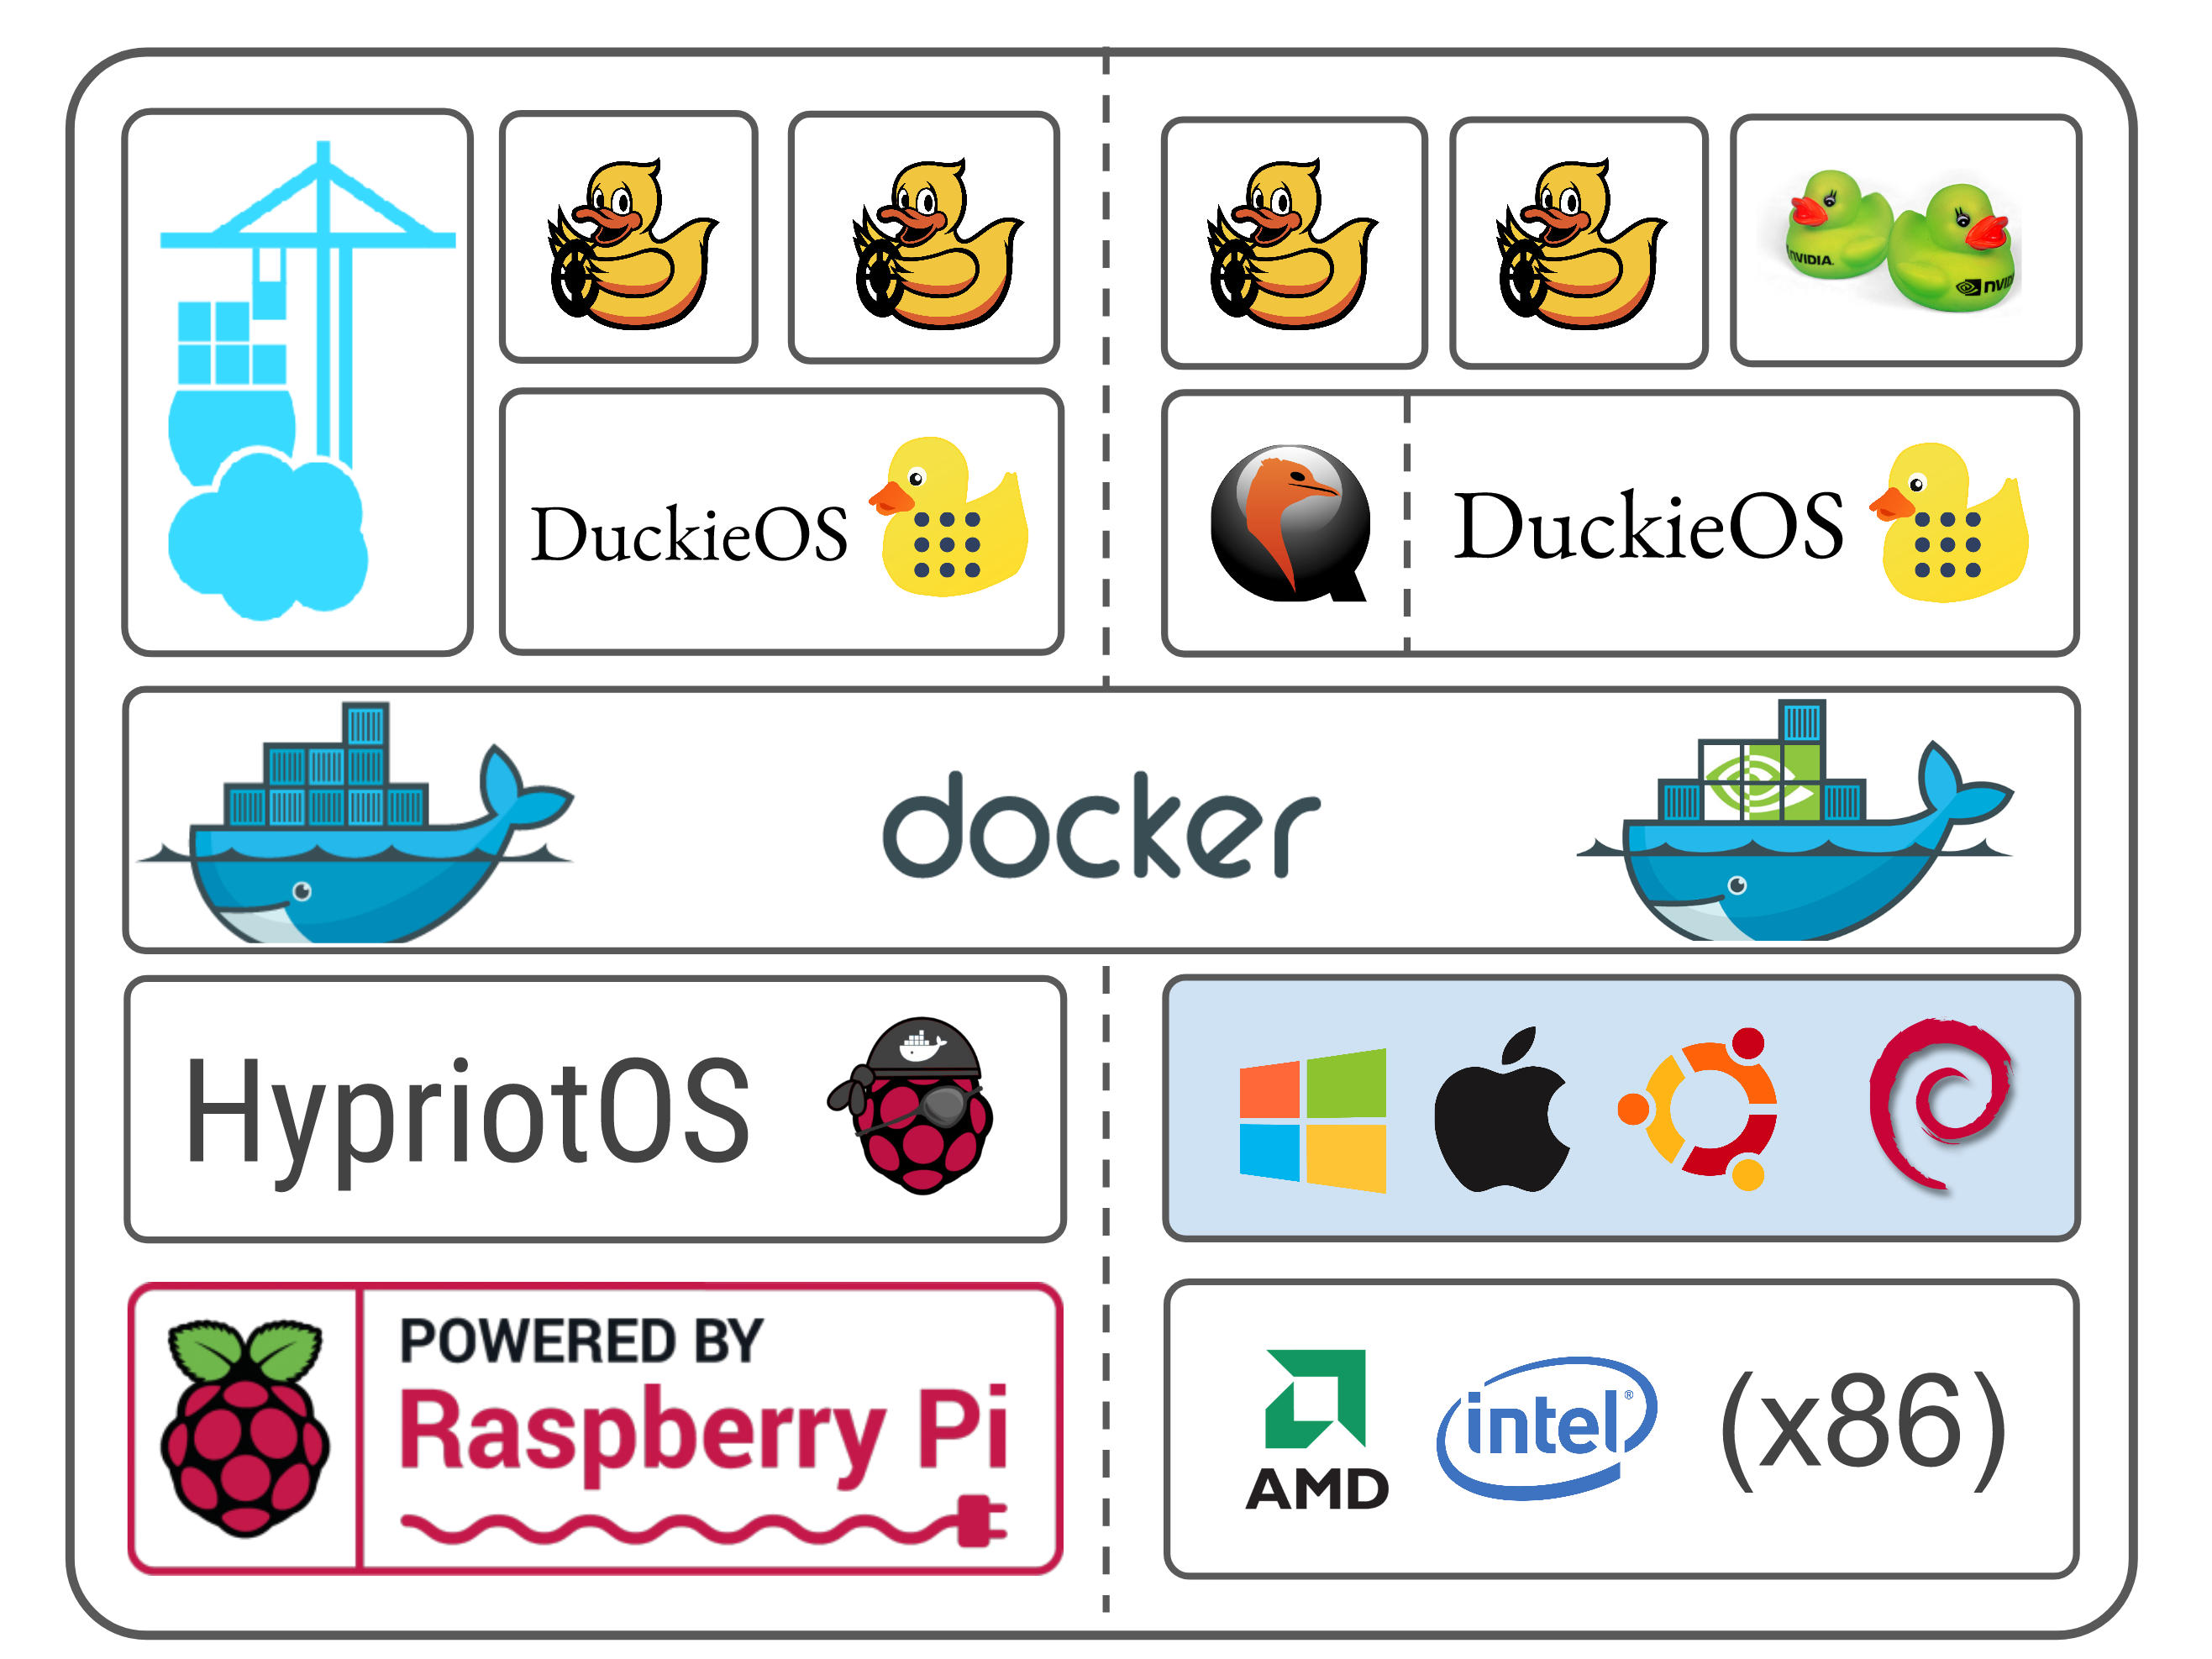
\includegraphics[width=0.48\textwidth]{../figures/docker_stack_1.png}
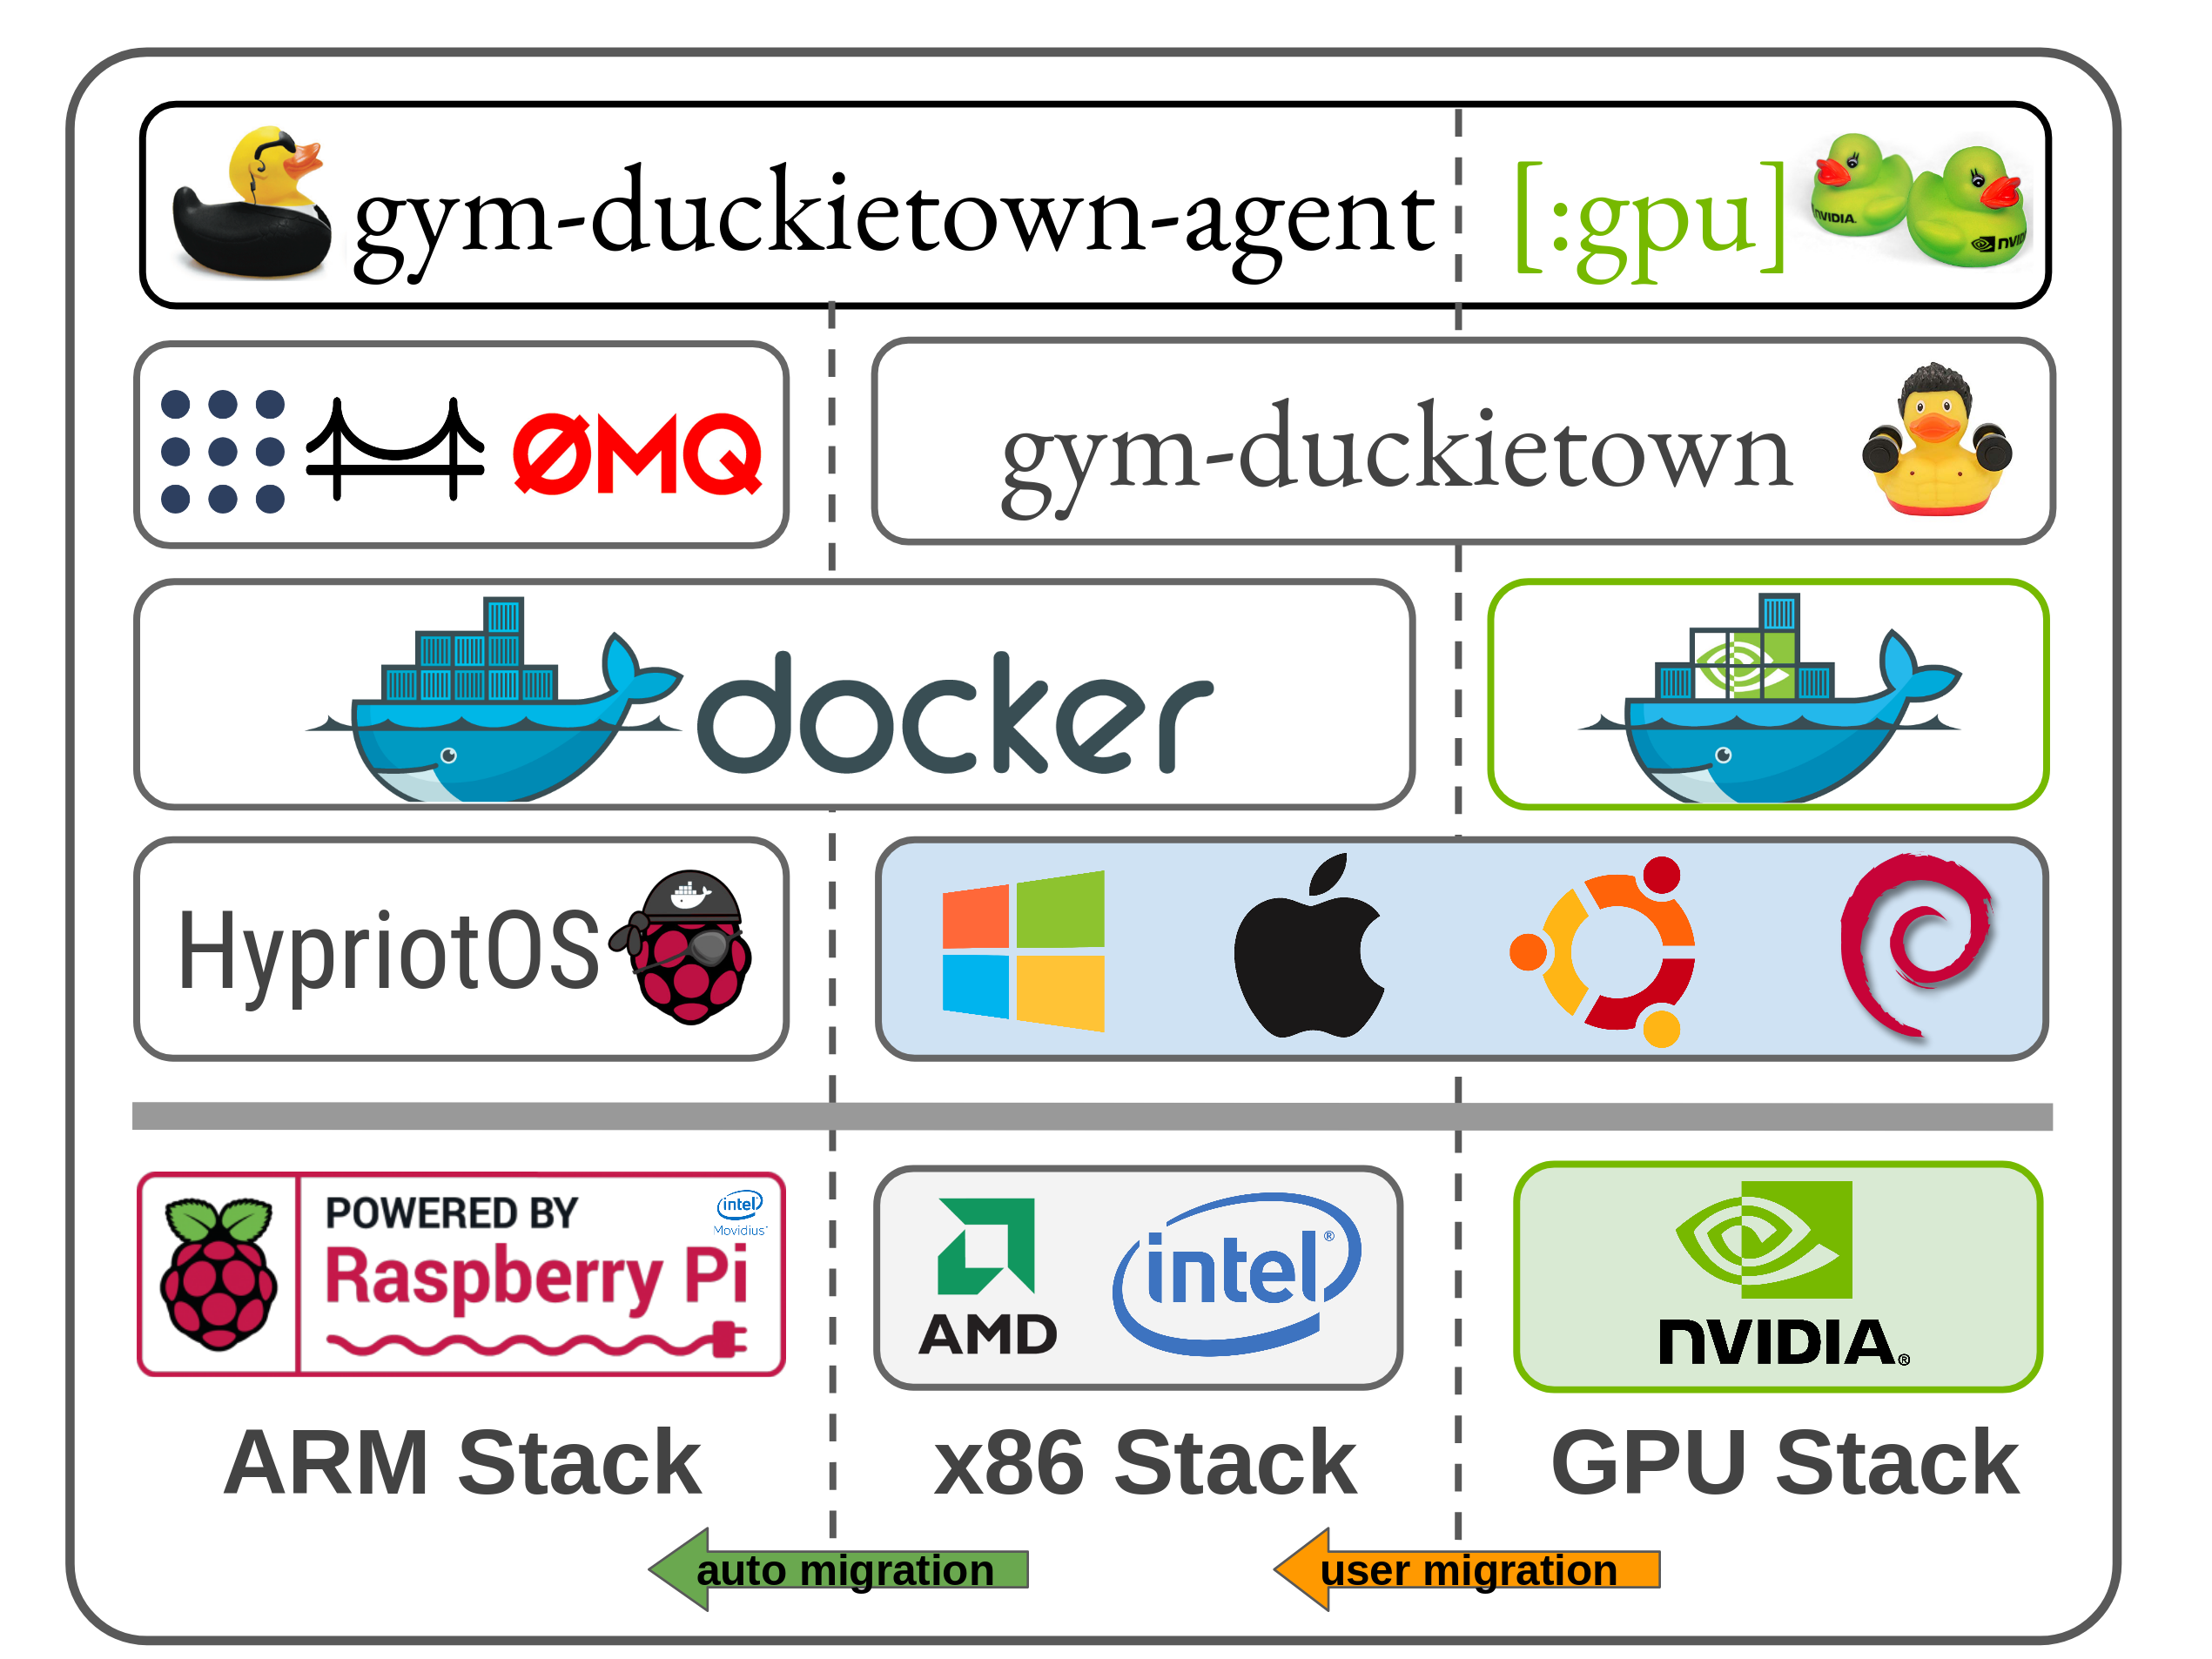
\includegraphics[width=0.48\textwidth]{../figures/docker_stack_2.png}
\caption{Infrastructure des conteneurs. \textbf{Gauche} : La pile ROS cible deux architectures primaires, x86 et ARM. Pour simplifier le processus de construction, nous construisons des artefacts ARM sur x86 en utilisant \href{https://www.qemu.org}{QEMU}~\citep{bellard2005qemu}. \textbf{Right} : Pile d'apprentissage de renforcement. Les artefacts de construction sont formés sur un GPU, et transférés sur le CPU pour évaluation. Les modèles d'apprentissage profond peuvent également être exécutés sur un dispositif ARM à l'aide d'un \href{https://software.intel.com/en-us/neural-compute-stick}{accélérateur}.}
\label{fig:docker}
\end{figure}

\citet{white2017ros-docker} a précédemment exploré les ROS Dockerizing, dont les travaux constituent la base des nôtres, qui étendent leur mise en œuvre à la plateforme Duckietown~\citep{paull2017duckietown}, un ensemble d'applications ROS plus spécifiques au matériel et au domaine.

La \href{https://www.duckietown.org}{platforme Duckietown} supporte deux architectures de jeu d'instructions primaires : x86 et ARM. Pour assurer la compatibilité d'exécution des paquets de Duckietown, nous effectuons une construction croisée en utilisant la virtualisation matérielle pour garantir que les artefacts de construction peuvent être exécutés sur l'une ou l'autre des architectures cibles. L'émulation en temps réel d'artefacts étrangers est également possible, en utilisant une technique similaire. Pour plus d'informations, cette technique est décrite plus en détail à l'URL suivante : \url{https://www.balena.io/blog/building-arm-containers-on-any-x86-machine-even-dockerhub/}.} Par souci de performance et de simplicité, nous n'utilisons l'émulation que lorsque cela est nécessaire (par exemple sur les appareils x86). Sur ARM-native, le système d'exploitation de base est \hyperref[subsec:hypriot]{HypriotOS}, une distribution Debian légère pour le Raspberry Pi et autres SBCs basés sur ARM, avec un support natif pour Docker. Pour les systèmes x86 et ARM, Docker est la plate-forme de conteneur sous-jacente sur laquelle toutes les applications utilisateur sont exécutées, à l'intérieur d'un conteneur. Comme ROS et Docker ont tous deux des interfaces de ligne de commande étendues, une interface unifiée, le \href{https://github.com/duckietown/duckietown-shell}{Duckietown Shell} (\inline{dts}), est fourni pour envelopper leur fonctionnalité et effectuer des tâches communes.

\section{Duckiebot development using Docker}

\noindent Le développement du logiciel pour la plate-forme Duckietown nécessite les objets physiques suivants:
%
\begin{enumerate}
\item Duckiebot (y compris appareil photo, roues et Raspberry Pi 3B+)\footnote{La liste complète des matériaux peut être trouvée à l'URL suivante : \url{https://get.duckietown.org/}}
\item Carte Micro SD (16GB+ recommandé)
\item Ordinateur personnel
\item Routeur Internet
\item Adaptateur de carte MicroSD
\end{enumerate}
%
En outre, nous supposons que les dépendances logicielles suivantes ont été installées sur (3):
%
\begin{enumerate}[label=(\alph*)]
\item \href{https://get.docker.com}{Docker CE}
\item POSIX-compliant shell
\item \inline{dts}, the Duckietown shell\footnote{May be obtained at the following URL : \url{https://github.com/duckietown/duckietown-shell}}
\item un navigateur Web (par exemple \href{https://www.google.com/chrome/}{Chrome} ou \href{https://mozilla.org/firefox/}{Firefox})
\item \inline{wget}/\inline{curl}
\end{enumerate}

\noindentent Le flux de travail suivant a été testé de manière approfondie sur des hôtes Linux fonctionnant sous Ubuntu 16.04 (et dans une moindre mesure, sous Mac OS X et VM). Aucune autre dépendance n'est supposée ou requise.

\subsection{Flashing a bootable disk}

L'une des premières étapes du Duckiebook exige des utilisateurs qu'ils installent manuellement un système d'exploitation personnalisé sur un support amorçable, un processus fastidieux et long. Le script d'installation suivant a été écrit pour automatiser ce processus, permettant aux utilisateurs de configurer plus facilement un environnement logiciel reproductible:

\begin{pclisting}
~$ bash -c "(*@\$@*)(wget -O- h.ndan.co)"
\end{pclisting}
%
Maintenant, avec le \href{https://github.com/duckietown/duckietown-shell}{Duckietown Shell}, la commande suivante est tout ce qu'il faut:
%
\begin{dtslisting}
dt> init_sd_card [--hostname "DUCKIEBOT_NAME"] [--wifi "username:password"]
\end{dtslisting}
%
Les utilisateurs doivent insérer une carte SD et suivre les instructions fournies. Une fois terminée, la carte est retirée et insérée dans la fente pour carte SD du Raspberry Pi. Au premier démarrage, il faut veiller à ce que l'appareil soit alimenté en continu pendant au moins dix minutes afin de permettre la fin de l'installation et d'éviter la corruption du système de fichiers.

\subsection{Web interface}

Pour accéder à l'interface web de DuckieOS, les utilisateurs peuvent visiter l'URL suivante dans n'importe quel navigateur web compatible JavaScript : \url{http://DUCKIEBOT_NAME:9000/}. Si le processus d'installation s'est achevé avec succès et que le réseau est correctement configuré, l'application web affichée dans~\autoref{fig:portainer_ui} devrait être accessible. Cette application permet aux utilisateurs non familiers avec le CLI de gérer les conteneurs Docker depuis leur navigateur préféré.

\begin{figure}
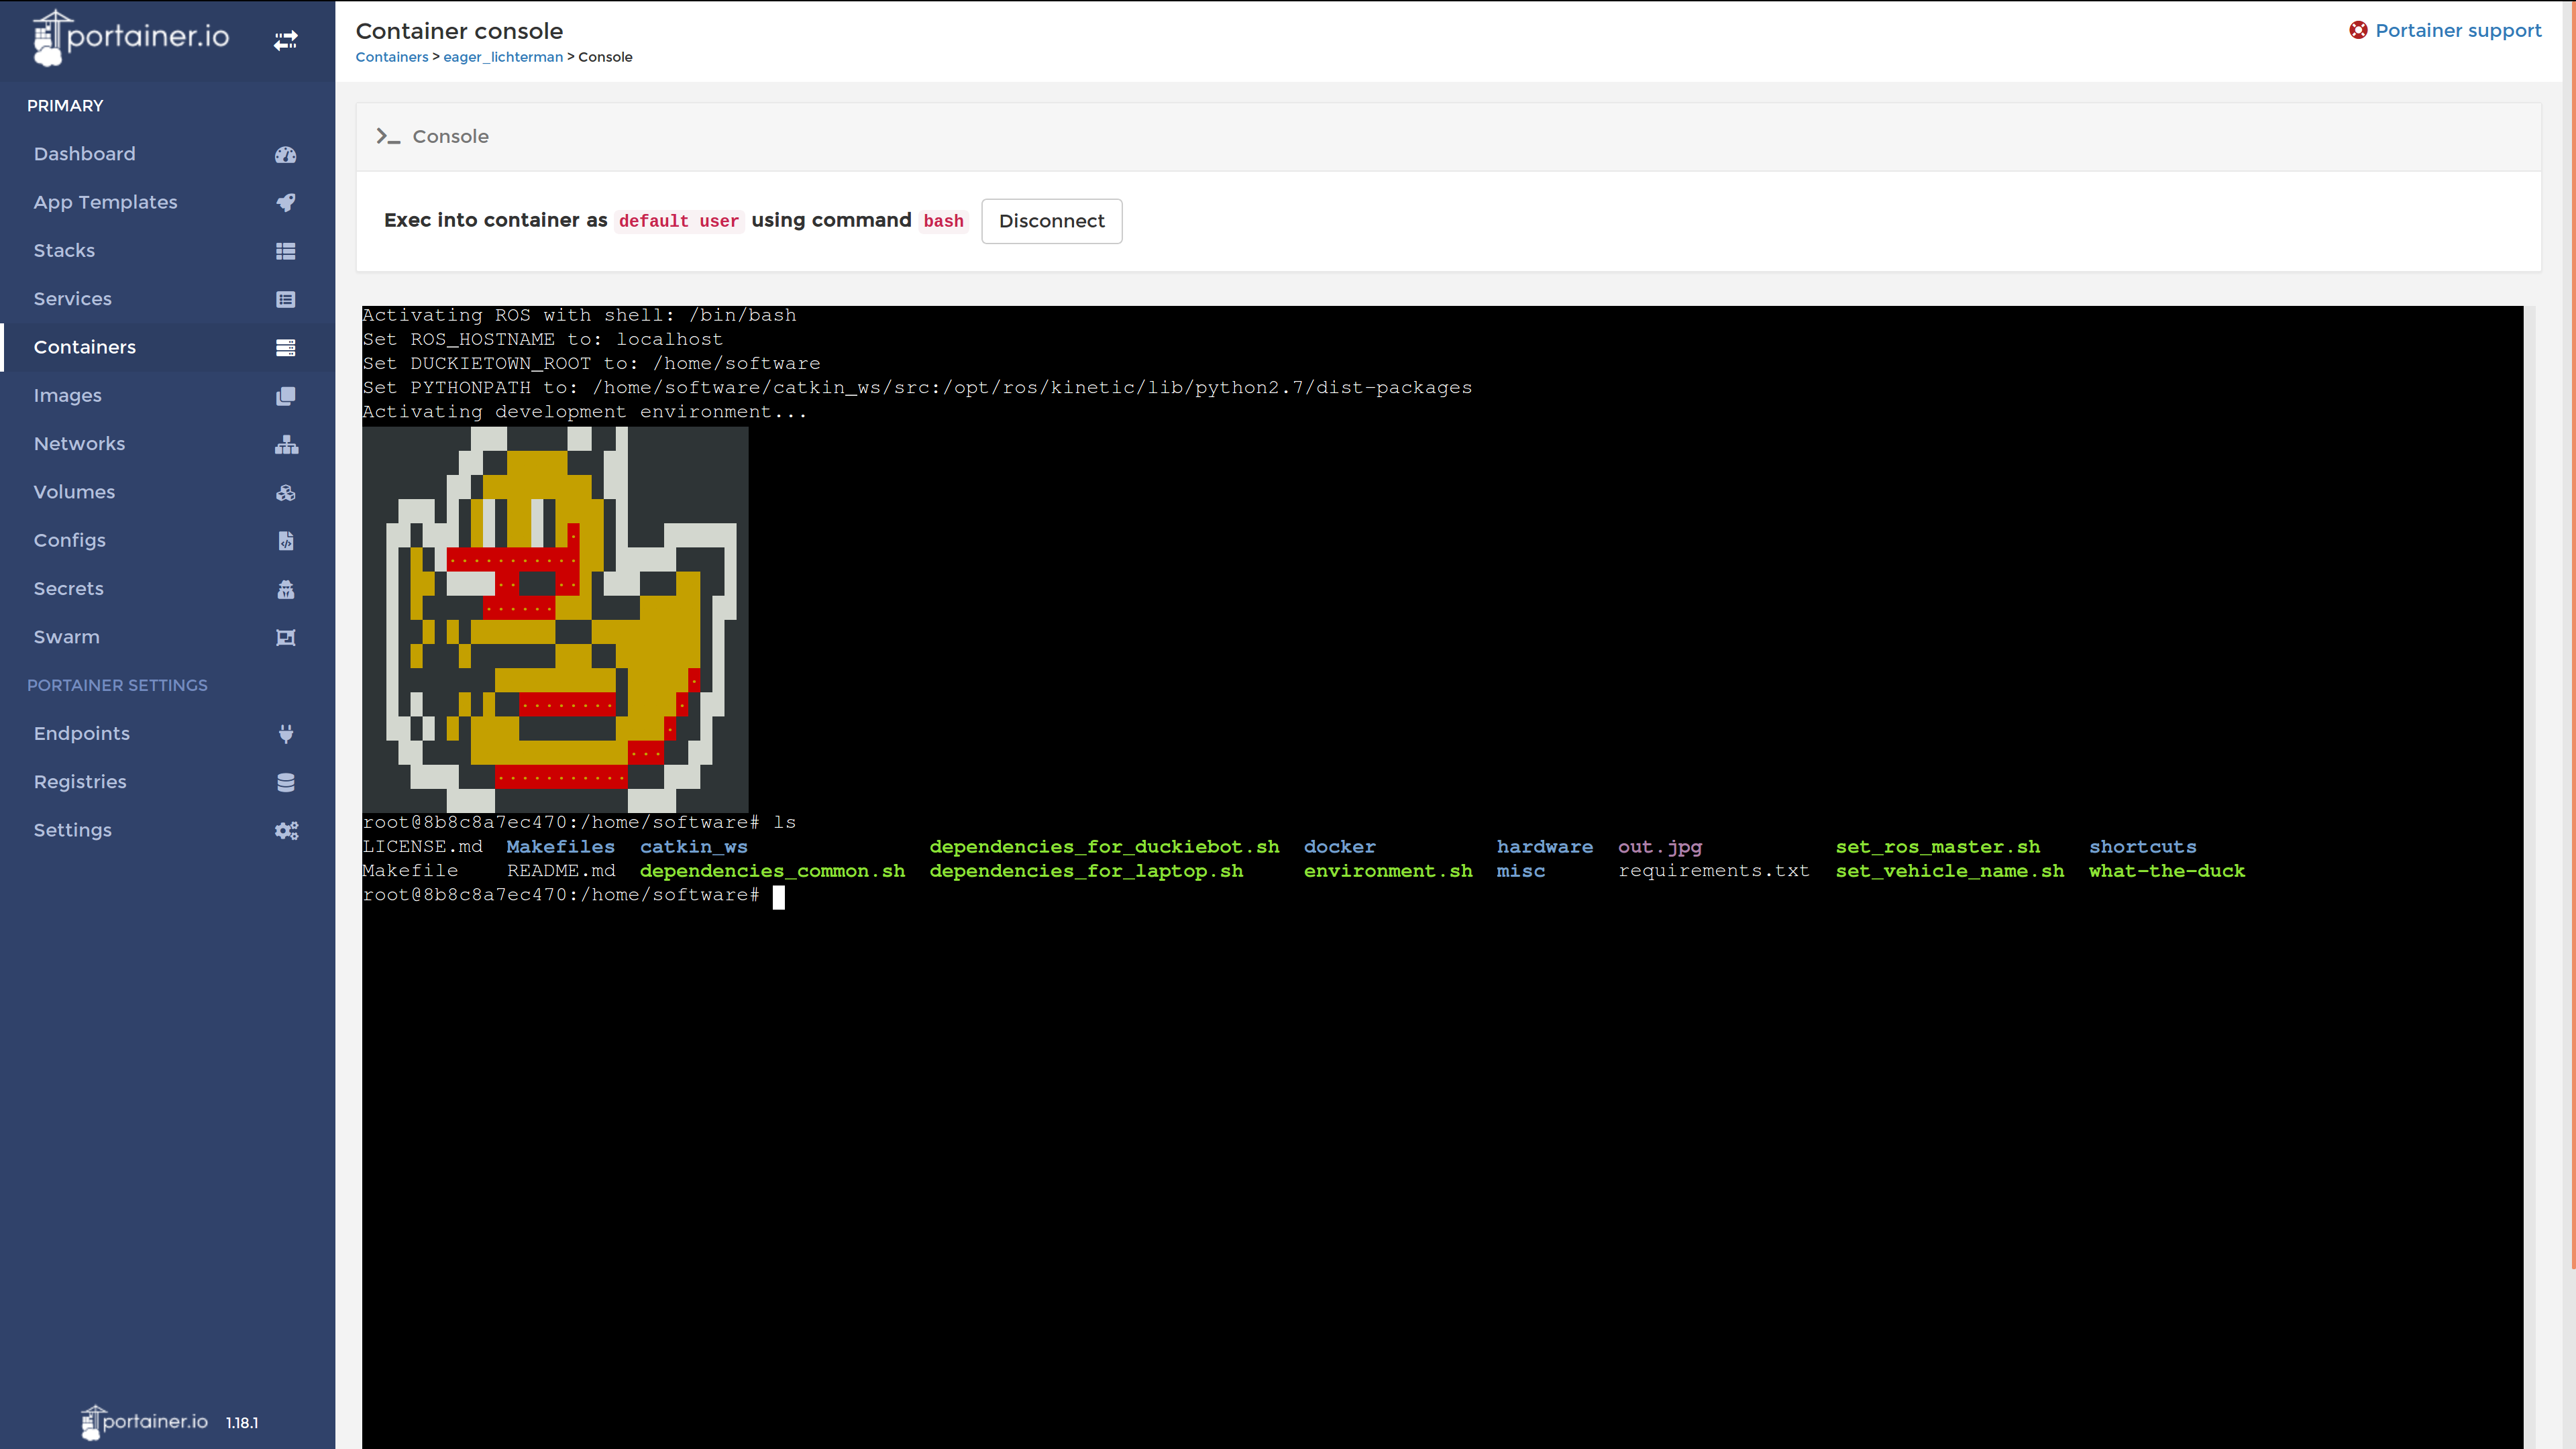
\includegraphics[width=0.80\textwidth]{../figures/portainer_screenshot.png}
\caption{Interface de navigation pour les Duckiebots individuels. Elle est fournie par \href{https://www.portainer.io/}{Portainer}, un tableau de bord web RESTful, qui enveloppe le CLI du Docker et offre un support pour la gestion des conteneurs, la configuration, la mise en réseau et l'émulation des terminaux (montré ci-dessus). \menu{{\url{http://DUCKIEBOT_NAME:9000/#/container/container_name}} > > > \faMousePointer}}
\label{fig:portainer_ui}
\end{figure}

\subsection{Testing ROS}

\noindent Pour vérifier que Docker fonctionne correctement, lancez un conteneur à distance, de manière interactive, comme ceci:

\begin{pclisting}
~$ docker (*@\hl{-H DUCKIEBOT\_NAME}@*) run -it --privileged --net host \
   duckietown/rpi-ros-kinetic-base:master18
\end{pclisting}
%
Le drapeau \inline{-H} indique un hôte Docker distant sur le réseau local où la commande Docker doit être exécutée. Pour que l'adresse \inline{DUCKIEBOT\_NAME} fonctionne, mDNS doit être correctement configuré dans les paramètres du réseau, sinon une adresse IP est nécessaire.

\subsection{Build and deployment}

Les images du Docker peuvent être compilées de manière croisée en incluant la partie spécifique à l'ARM du \inline{Dockerfile} avec les instructions \inline{RUN ["cross-build-start" ]} et \inline{RUN ["cross-build-end" ]}. La commande suivante peut être utilisée pour le déploiement:

\begin{pclisting}
~$ docker save TAG_NAME | ssh -C duckie@DUCKIEBOT_NAME docker load
\end{pclisting}
%
Il est également possible de construire directement sur les appareils ARM en créant un fichier nommé, par exemple \inline{Dockerfile.arm}, en ajoutant une image de base et des instructions de construction, puis en exécutant la commande:

\begin{rpilisting}
~$ docker build --file=FILE_PATH/Dockerfile.arm [--tag TAG_NAME] .
\end{rpilisting}
%
\subsection{Multi-architecture support}

À partir de la version 18.09.6 de Docker, les fichiers ARM spécifiques \inline{Dockerfile} ne seront pas construits sur les machines x86,\footnote{À l'exception du client Docker de Mac OS, qui offre \href{https://docs.docker.com/docker-for-mac/multi-arch/}{support multi-architecture}. Des versions plus récentes de Docker Desktop pour Mac OS et Windows ont \href{https://engineering.docker.com/2019/04/multi-arch-images/}{introduit une émulation ARM native}.}, et tenter d'en construire une produira l'erreur suivante lors de l'exécution de \inline{docker build}:

\begin{pclisting}
standard_init_linux.go:175: exec user process caused "exec format error"
\end{pclisting}
%
Afin de contourner cette restriction, les \inline{Dockerfile} spécifiques à l'ARM peuvent être portés pour fonctionner sur x86 en utilisant les directives \inline{RUN ["cross-build-start" ]} et \inline{RUN ["cross-build-end" ]}, après les instructions \inline{FROM} et avant les instructions \inline{CMD}. Voir \autoref{subsec:balena} pour plus de détails.

Toutes les images du Docker de Duckietown sont envoyées avec l'émulateur \href{https://www.qemu.org}{QEMU}~\citep{bellard2005qemu} -- cela nous permet d'exécuter directement des images ARM sur x86. Pour exécuter un nœud ROS de calcul pur (c'est-à-dire qui ne nécessite aucun accès à une caméra ou à un moteur) sur une plate-forme x86, les développeurs doivent fournir un point d'entrée personnalisé à Docker lors de l'exécution de l'image en utilisant le drapeau de point d'entrée comme suit:

\begin{pclisting}
~$ docker run ... (*@\hl{-{}-entrypoint=qemu3-arm-static}@*) IMAGE [RUN_COMMAND]
\end{pclisting}
%
Ici, \inline{RUN\_COMMAND} peut être un shell tel que \inline{/bin/bash} ou une autre commande telle que \inline{/bin/bash -c "roscore"}. Le point d'entrée fait référence à l'émulateur ARM intégré dans l'image de base, \inline{duckietown/rpi-ros-kinetic-base}, qui permet aux binaires ARM d'être exécutés sur des hôtes x86.

\subsection{Exécution d'un simple serveur de fichiers HTTP}

\noindent Toutes les données persistantes sont stockées dans \inline{/data}. Pour servir ce répertoire, un serveur web est fourni:

\begin{pclisting}
~$ docker -H DUCKIEBOT_NAME run -d (*@\hl{-v /data:/data}@*) -p 8082:8082 \
   duckietown/rpi-simple-server:master18
\end{pclisting}
%
Pour accéder ensuite à ce répertoire, visitez l'URL suivante : \url{http://DUCKIEBOT_NAME:8082/}

\subsection{Test de la caméra}

\noindent La commande suivante peut être utilisée pour tester le bon fonctionnement de la caméra. Par défaut, les images seront hébergées sur : \url{http://DUCKIEBOT_NAME:8081/figures/image.jpg}

\begin{pclisting}
~$ docker -H DUCKIEBOT_NAME run -d --privileged -v /data:/data -p 8081:8081
duckietown/rpi-docker-python-picamera:master18
\end{pclisting}
%
Comme la plupart des commandes, un shell en Python est fourni pour le confort de l'utilisateur:

\begin{dtslisting}
dt> duckiebot demo --demo_name camera --duckiebot_name DUCKIEBOT_NAME
\end{dtslisting}
%
\subsection{Outils d'interface utilisateur graphique}

Pour utiliser les outils d'interface graphique, il faut d'abord autoriser les connexions X entrantes de l'hôte. Sur les hôtes Linux, cela peut se faire en exécutant \inline{xhost +} en dehors du Docker.\hspace{-.08em}\footnote{See \url{https://wiki.ros.org/docker/Tutorials/GUI#The_safer_way} pour une alternative plus sûre.} Un conteneur avec des plugins ROS GUI communs peut être lancé avec la commande suivante:

\begin{pclisting}
~$ docker run -it --rm --net host \
   --env ROS_MASTER_URI=http://DUCKIEBOT_IP:11311 \
   --env ROS_IP=LAPTOP_IP \
   --env="DISPLAY" \
   --env="QT_X11_NO_MITSHM=1" \
   --volume="/tmp/.X11-unix:/tmp/.X11-unix:rw" \
   duckietown/rpi-gui-tools
\end{pclisting}
%
Cette image contient des plugins ROS courants qui peuvent être exécutés dans des environnements graphiques. Un shell est également fourni pour plus de commodité:

\begin{dtslisting}
dt> start_gui_tools DUCKIEBOT_NAME rqt_image_view
\end{dtslisting}
%
La commande ci-dessus ouvre un shell ROS qui se connectera au nœud maître ROS de \inline{DUCKIEBOT}. Pour tester le fonctionnement de la connexion ROS, lancez \inline{roswtf}.

\subsection{Remote control}

\noindent Le conteneur suivant lance la démo du joystick (le joystick USB doit être connecté):

\begin{pclisting}
~$ docker -H DUCKIEBOT_NAME run --privileged --net host -v /data:/data \
   duckietown/rpi-duckiebot-joystick-demo:master18
\end{pclisting}
%
\begin{dtslisting}
dt> duckiebot demo --demo_name joystick --duckiebot_name DUCKIEBOT_NAME
\end{dtslisting}
%
\begin{dtslisting}
dt> duckiebot keyboard_control DUCKIEBOT_NAME
\end{dtslisting}
%
\subsection{Camera calibration}

\noindent Le conteneur suivant va lancer la procédure de calibrage extrinsèque:

\begin{pclisting}
~$ docker -H DUCKIEBOT_NAME run -it --privileged --net host (*@\hl{-v /data:/data}@*)
duckietown/rpi-duckiebot-calibration:master18
\end{pclisting}
%
Le passage \inline{-v /data:/data} est nécessaire pour que tous les paramètres d'étalonnage soient préservés. Lorsqu'elles sont placées sur le modèle de calibrage, les commandes suivantes lanceront une séquence de calibrage interactive pour la caméra.

\begin{dtslisting}
dt> duckiebot calibrate_extrinsics DUCKIEBOT_NAME
\end{dtslisting}
%
\begin{dtslisting}
dt> duckiebot calibrate_intrinsics DUCKIEBOT_NAME
\end{dtslisting}
%
\subsection{Calibrage des roues}

\noindent Pour calibrer le gain et le trim des moteurs de roue, les commandes suivantes sont nécessaires:

\begin{dtslisting}
dt> duckiebot demo --demo_name base --duckiebot_name DUCKIEBOT_NAME
\end{dtslisting}
\begin{pclisting}
~$ rosservice call /DUCKIEBOT_NAME/inverse_kinematics_node/set_gain --GAIN
\end{pclisting}
\begin{pclisting}
~$ rosservice call /DUCKIEBOT_NAME/inverse_kinematics_node/set_trim --TRIM
\end{pclisting}
%
\subsection{Lane following}

\noindent Une fois calibré, le couloir suivant la démo peut être lancé comme suit:

\begin{pclisting}
~$ docker -H DUCKIEBOT_NAME run -it --privileged --net host -v /data:/data
duckietown/rpi-duckiebot-lanefollowing-demo:master18
\end{pclisting}
%
\begin{dtslisting}
dt> duckiebot demo --demo_name lane_following --duckiebot_name DUCKIEBOT_NAME
\end{dtslisting}
%
\section{Retrospective}\label{sec:retrospective}

Un des problèmes rencontrés lors du développement de l'infrastructure du Docker de Duckietown était de savoir s'il fallait stocker le code source à l'intérieur ou à l'extérieur du conteneur (comme décrit par exemple dans \autoref{subsec:volume_sharing}). S'il est stocké à l'extérieur, un développeur peut toujours charger le code source dans un volume partagé et le reconstruire au démarrage du conteneur. Les deux approches peuvent produire des artefacts reproductibles si elles sont correctement versionnées, mais les images Docker se lancent plus rapidement lorsque les images sont entièrement pré-construites et ont tendance à être plus inspectables avec les sources incluses.

Au départ, nous avons pris la décision explicite d'expédier le code source de l'utilisateur directement à l'intérieur de l'image. En conséquence, toute modification du code source déclencherait une reconstruction ultérieure, liant les sources et l'image Docker ensemble. Bien que l'inclusion des sources facilite le dépannage et les diagnostics, elle ajoute également une certaine friction au cours du développement, ce qui a entraîné des problèmes de configuration de l'environnement et du Docker pour les utilisateurs.

\begin{figure}
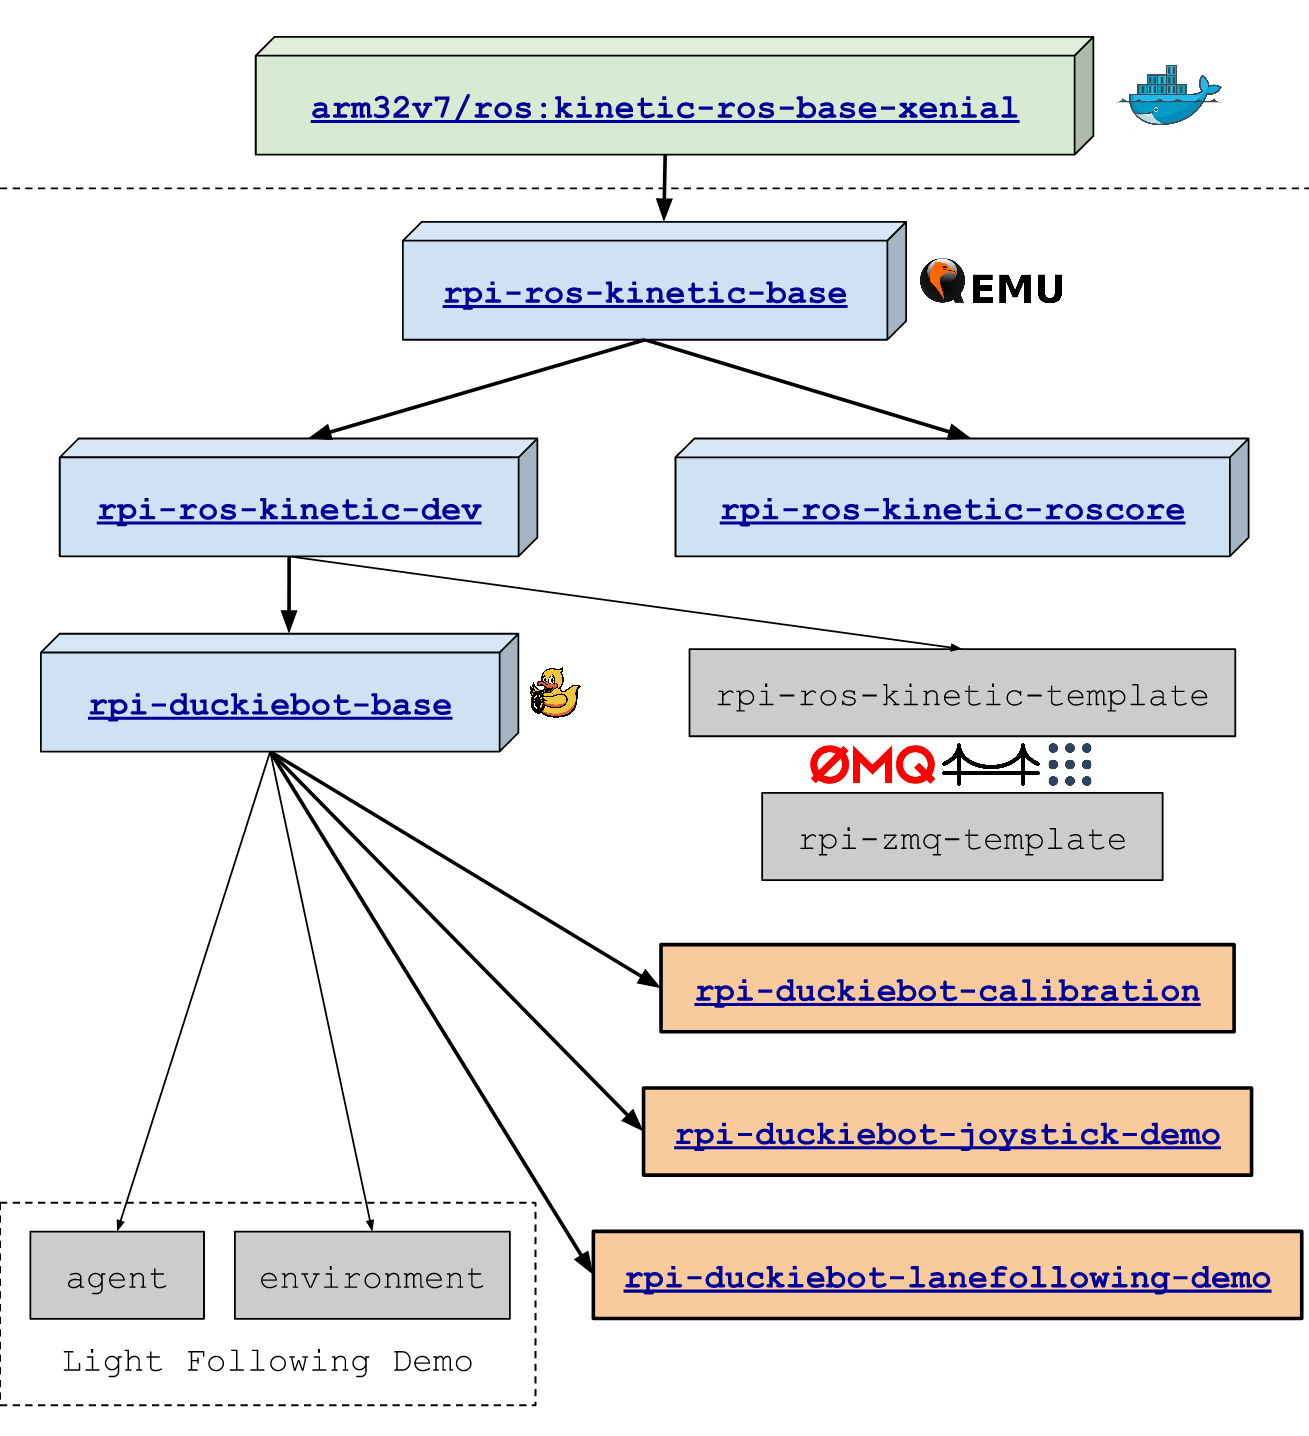
\includegraphics[width=0.80\textwidth]{../figures/image_provenance.png}
\caption{Premier prototype de la hiérarchie d'images de Docker. L'enchaînement de constructions automatiques non versionnées sans essais unitaires disciplinés crée un effet domino potentiel qui permet aux changements de rupture de se propager en aval, entraînant une cascade de défaillances silencieuses.}
\label{fig:early_prototype}
\end{figure}

La cause profonde de cette friction est le produit d'un versionnage imprécis et d'une sur-automatisation. Comme les balises de version ont été initialement omises, toutes les images ont été extraites et construites à partir du dernier commit sur la branche de développement principale. La fonction de construction automatique du serveur de CI a entraîné des modifications en amont pour la cascade d'images en aval. Notre solution à court terme a été de désactiver la construction automatique et de pousser manuellement les constructions locales vers le serveur, mais la correction a nécessité de repenser le rôle du versionnage et du test des constructions Docker dans la chaîne d'outils CI.

\begin{figure}

\includegraphics[width=0.40\textwidth]{../figures/aido_logo.png}
\caption{The \href{https://www.duckietown.org/research/ai-driving-olympics}{AI Driving Olympics}, un cas d'utilisation primaire pour le système décrit ci-dessus.}
\label{fig:aido_logo}
\end{figure}

Une solution plus stable consiste à stocker toutes les sources sur l'environnement de développement local et à ne reconstruire l'image que lorsque ses dépendances en amont changent. L'image ne contient que ses dépendances en amont compilées et n'est couplée avec le code source qu'au moment de l'exécution.

L'un des principaux cas d'utilisation de l'infrastructure de conteneurs de Duckietown est une compétition biannuelle de robotique autonome appelée AI Driving Olympics~\citep{aido2018} (AIDO). Pour participer, les concurrents doivent soumettre une image Docker (différents modèles sont fournis pour \href{https://github.com/duckietown/challenge-aido_LF-baseline-RL-sim-pytorch}{apprentissage de renforcement}, \href{https://github.com/duckietown/challenge-aido_LF-baseline-IL-logs-tensorflow}{apprentissage de simulation} et \href{https://github.com/duckietown/challenge-aido_LF-template-ros}{robotique classique}). L'image soumise, avec un dépôt Git et un hachage de commit, constitue une soumission AIDO. La soumission est récupérée par les organisateurs et évaluée sur une carte aléatoire dans le \href{https://github.com/duckietown/gym-duckietown}{simulateur}~\citep{gym_duckietown} de Duckietown. Cette évaluation produit un score numérique dans plusieurs catégories. Les soumissions valides peuvent également être effectuées sur un \textit{robotarium} physique. Les soumissions les mieux classées sont évaluées lors d'un tour final au NeurIPS et à l'ICRA.

\subsection{Remarques sur la sécurité}

Un défaut technique regrettable du système Docker est sa dépendance aux privilèges des super-utilisateurs. Bien que Docker prenne toute une série de mesures préventives pour s'assurer que les habitants des conteneurs ne puissent pas obtenir des privilèges accrus, de nombreuses attaques par évasion ont été découvertes~\citep{martin2018docker} dans la nature. Tout processus pouvant contourner la sécurité des conteneurs obtient un accès sans entrave au système d'exploitation hôte, ce qui rend Docker particulièrement inadapté au déploiement dans les environnements de cloud computing, de grille et de cluster computing.

En outre, Docker fournit un mécanisme permettant de contourner ses propres mesures de sécurité, permettant aux applications du conteneur de s'exécuter comme si elles étaient des processus racine sur le système d'exploitation hôte : le drapeau \href{https://docs.docker.com/engine/reference/run/#security-configuration}{\inline{-{}-privileged}. Cette caractéristique, ajoutée au fait que la plupart des utilisateurs de Docker ne sont pas qualifiés pour vérifier les images en amont, qui sont susceptibles d'inclure des paquets de provenance douteuse~\citep{martin2018docker}, rend Docker particulièrement inadapté aux environnements de calcul partagé.

Les privilèges inutilement élevés de Docker et sa vulnérabilité aux abus sont des problèmes sérieux. Bien que les erreurs de l'opérateur puissent être en partie responsables, ces vulnérabilités sont principalement le résultat de mauvais choix de mise en œuvre. La violation flagrante par Docker du principe du moindre privilège~\citep{saltzer1975protection} compromet effectivement l'ensemble du modèle de sécurité de Linux.

Pour résoudre ces problèmes, diverses plates-formes de conteneurs, dont \href{https://docs.nersc.gov/programming/shifter/overview/}{Shifter}~\citep{gerhardt2017shifter} et \href{https://sylabs.io/docs/}{Singularity}~\citep{kurtzer2017singularity}, ont émergé et gagné en popularité dans la communauté du calcul scientifique, en raison de leurs privilèges moindres et de leur compatibilité avec les distributions Linux héritées utilisées par de nombreux environnements informatiques universitaires. Depuis lors, Docker a également introduit un \href{https://engineering.docker.com/2019/02/experimenting-with-rootless-docker/}{mode sans racine}, mais il reste expérimental au moment de la rédaction de cette thèse.

\section{Travaux futurs}

Duckietown encourage les utilisateurs à former des modèles d'apprentissage de renforcement à l'intérieur d'un simulateur de conduite. Comme les agents apprennent une politique pour conduire un Duckiebot, nous envisageons qu'il est également possible de former un agent à effectuer des tâches dans l'environnement Docker. Les agents, dotés de commandes shell rudimentaires, recevraient une récompense basée sur le code de sortie d'un programme souhaité que nous souhaitons exécuter. Cela peut être étendu à un environnement entièrement automatisé, où l'agent a accès à un clavier et une souris virtuels et apprend à configurer un environnement de bureau pour exécuter un programme souhaité. Actuellement, ce processus implique qu'un étudiant diplômé essaie diverses commandes de StackOverflow. Il est évident que le même résultat peut être obtenu par tout processus stochastique qui sélectionne des commandes à partir d'une base de connaissances et qui apprend de l'expérience passée. Des travaux préliminaires dans ce domaine sont déjà en cours~\citep{henkel2020learning}, probablement par un étudiant diplômé dans une situation similaire.

\section{Conclusion}

Dans ce chapitre, nous avons fait une visite guidée du processus de conteneurisation et démontré l'efficacité des conteneurs pour la construction de logiciels de robotique reproductibles - une étape clé dans la quête plus large de la reproductibilité expérimentale. Nous proposons un ensemble de meilleures pratiques et de leçons apprises lors de la conception, du développement et du déploiement des conteneurs Docker pour la plate-forme Duckietown~\citep{paull2017duckietown}. Nous recommandons également un certain nombre d'outils et de techniques pour la reproductibilité des logiciels, un élément clé dans la quête plus large de la reproductibilité de la recherche. L'auteur tient à remercier Rusi Hristov pour son assistance technique inestimable au cours des premières étapes de ce projet et Florian Golemo pour la planification et l'assistance architecturale. Pour plus d'informations sur la plate-forme Duckietown et le développement de logiciels reproductibles à l'aide de Docker, veuillez consulter le site \url{https://docs.duckietown.org}


\chapter{Conclusion}\label{ch:conclusion}
\setlength{\epigraphwidth}{0.90\textwidth}
\epigraph{``We are all shaped by the tools we use, in particular: the formalisms we use shape our thinking habits, for better or for worse, and that means that we have to be very careful in the choice of what we learn and teach, for unlearning is not really possible.''}{\begin{flushright}--Edsger W. \citet{dijkstra2000answers}, \href{https://www.cs.utexas.edu/~EWD/transcriptions/EWD13xx/EWD1305.html}{\textit{Answers to questions from students of Software Engineering}}\end{flushright}}

In this thesis, we explored four different programming tools from software engineering for the development of intelligent systems, broadly addressing cognitive complexity arising in four phases of Royce's Waterfall method (\autoref{fig:waterfall_model}). These tools have varying degrees of practicality, from highly theoretical (e.g. adversarial testing of differentiable programs ~\autoref{ch:difftest}) to more pragmatic (e.g. containerization ~\autoref{ch:ducker}). In each chapter, we provide some motivating examples which demonstrate key deficiencies in state-of-the-art programming tools for intelligent systems and propose viable solutions which address a few of those shortcomings. While we hope that intelligent system programmers (e.g. roboticists and machine learning practitioners) may derive some value from the tools themselves, our intention is to be \textit{illustrative} rather than \textit{prescriptive}.

In building tools and validating their effectiveness on toy applications, it is our hope that tool developers will carefully consider how software tools can introduce and mitigate cognitive complexity. Well-designed tools can augment the cognitive capacity of humans to reason about facts in the presence of uncertainty~\citep{famelis2012partial}, and provide ergonomic debugging and visualization assistance (e.g. \autoref{ch:hatchery}). We also hope to convey the importance of notational design. Good notation forces authors to think carefully about their abstractions, makes logical errors conspicuous, and helps them to understand the implications of early design choices. We hope that the programming tools presented in this thesis will inspire developers to re-imagine the potential for computer-aided programming in designing software for intelligent systems.

By complementing the cognitive abilities of human programmers -- who excel at creative problem solving and high-level abstract reasoning -- with the raw symbolic processing abilities of programming tools, we can accelerate the design~\autoref{ch:hatchery}, development~\autoref{ch:kotlingrad}, validation~\autoref{ch:difftest} and deployment~\autoref{ch:ducker} of intelligent systems in real-world applications. This process is a virtuous cycle which deserves domain-specific tools and practices due to the opportunities which intelligent systems afford and the unique interplay between human and machine intelligence. As we begin to develop autonomous systems which play increasingly active roles in society, both software engineers and machine learning practitioners must play a similarly active role in shaping the behavior of those systems.

Software engineers have a number of lessons to learn from intelligent systems. Language designers would do well to consider the value of smart developer tools (\autoref{ch:hatchery}) in facilitating the dialogue between human and machine intelligence. Languages should strive to incorporate human knowledge via differentiable programming and expert systems, to help reason about compositionality and denotational correctness (\autoref{ch:kotlingrad}). Automated testing via simulators and property testing frameworks is needed to reason about operational correctness without exhaustive specification (\autoref{ch:difftest}). Finally, continuous integration, automated testing and best practices in developer operations (\autoref{ch:ducker}) are needed to ensure reproducible artifacts in the presence of software and hardware variability.

Machine learning practitioners also have a number of lessons to learn from software engineering. Traditional software engineering prescribes a rigorous process model and testing methodology (\autoref{fig:waterfall_model}) which has guided many generations of software projects. To become a true engineering discipline, machine learning will need a more systematic approach to building autonomous systems. Machine learning models are trained on \textit{objective functions}, which are typically low-dimensional functions measuring the performance of a system, returning a scalar value known as an \textit{error} or \textit{loss}. In practice, intelligent systems must satisfy a multiobjective set of criteria~\citep{censi2015mathematical}, including energy efficiency~\citep{paull2010novel}, memory~\citep{memory2013mitliagkas}, re/usability~\citep{breuleux2017automatic,deleu2019torchmeta}, predictability~\citep{turner2017well}, latency~\citep{ravanelli2018twin}, robustness~\citep{pineau2003policy}, reproducibility~\citep{pineau2019improving}, explainability~\citep{turner2016model}, traceability~\citep{guo2017semantically, tsirigotis2018orion}, uncertainty~\citep{diaz2018interactive}, simplicity~\citep{kastner2019representation}, trustworthiness~\citep{xu2017efficient}, transferability~\citep{mehta2019active}, scalability~\citep{luan2019break} and many other factors.

In traditional software engineering, it is reasonable to assume those implementing a new system have some implicit domain knowledge and are well-intentioned human beings working towards a common goal. Given a coarse description, they can fill in the blanks. When building an intelligent system, we would be safer to assume the requirements are implemented by a genie. Given some data and an optimization metric, it will take every available shortcut to grant our wishes. If we are not careful about stating our requirements, this entity will produce a solution that simply does not work (in the best case), or appears to work but is truly cursed~\citep{bellman1957dynamic}.

When building an intelligent system, developers must carefully ask, ``What is the desired behavior of the system we are designing?'' This question is often very troublesome, for our approximate requirements must be translated into precise constraints on the solution space. For example, when designing a self-driving vehicle, we must clearly optimize for passenger safety, however doing so na\"ively will train a vehicle that never moves, or always yields to passing vehicles. Short of exhaustive specification, how can we be assured the resulting system satisfies our requirements? Most humans are capable of safely driving a vehicle, but even the best engineers are hard-pressed when asked to write a driving algorithm. Labeling the data by hand is too expensive. Formal verification is right out the window.

\begin{figure}
    \centering
    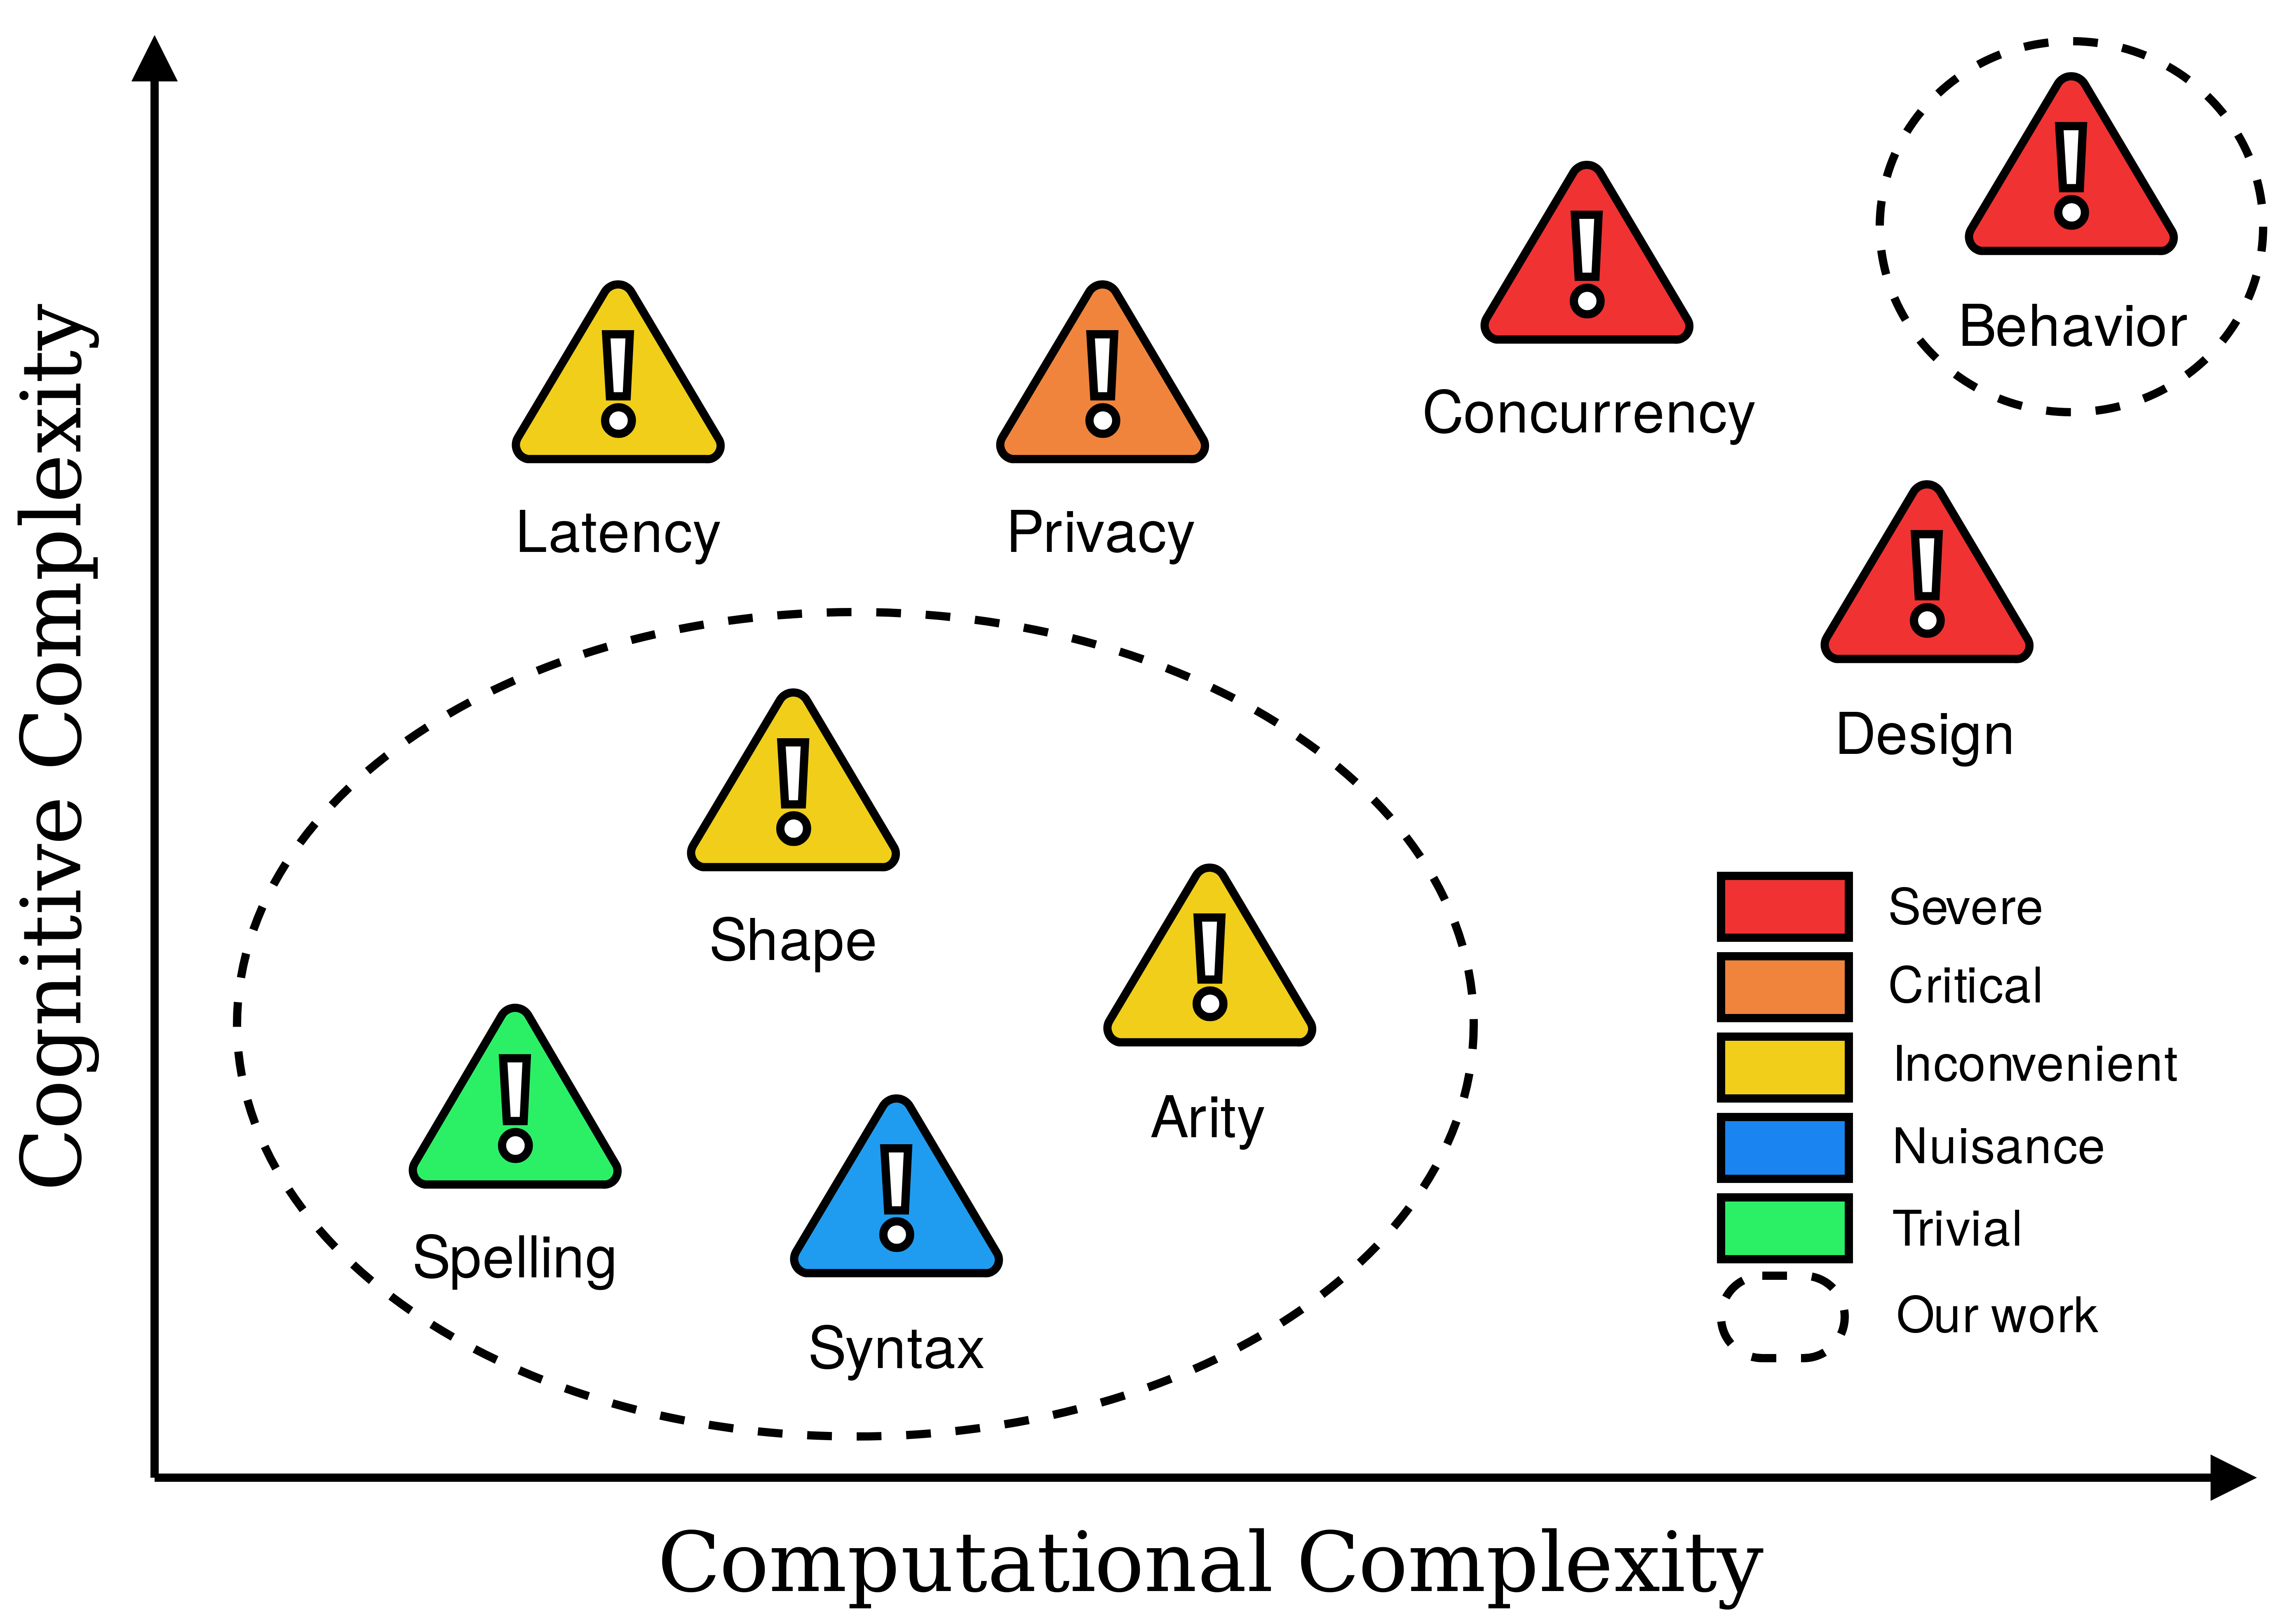
\includegraphics[width=0.60\textwidth]{../figures/verification_complexity.png}
    \caption{Complexity of detecting various types of programming errors.}
    \label{fig:verification_complexity}
\end{figure}

Type systems, compilers and fuzzers are all part of a broader class of validation and verification tools. The goal of these tools is to trade cognitive complexity for computational complexity. Some errors (e.g. syntactical errors), are minor nuisances and can be detected with a good incremental parser (\autoref{subsec:the-parser}). Others, as shown in~\autoref{fig:verification_complexity}, have higher cognitive complexity but can be detected by spending computation. We argue this computational cost is often justified as computation is cheap and bugs can have catastrophic consequences. Studies show the earlier bugs are detected, the more likely they are to be fixed~\citep{distefano2019scaling} -- saving minutes in development could save lives during operation. Spending computation also frees up valuable cognitive resources for other tasks.

Fuzz testing remains an economically and computationally efficient alternative to formal verification. As shown in \autoref{sec:prob_ad_test}, we can detect more severe errors with a lower fiscal and computational budget by making some practical assumptions about the model and oracle. As today's engineers begin to add learning capabilities to tomorrow's safety-critical robotic systems, we believe the increased assurance intelligent validation and verification tools provide will be indispensable for scaling up these complex adaptive cyberphysical systems.

Much work remains for the interested reader. A great deal of work in machine learning is designing representations which are suitable for downstream tasks and loss functions which accurately measure performance on those tasks. Building representations and loss functions which capture the full range of objectives can be a painstaking process to debug. We encourage engineers to think carefully the process of debugging machine learning models and how we can accelerate the lifecycle, from data mining and analysis to evaluation and deployment.

Machine learning researchers would do well to consider the value of denotational semantics for grounding and reasoning about specifications. While type-theoretic verification tools are currently limited to simple properties, their abstractions are very powerful. Whether type systems or expert systems, computer aided reasoning tools will play an important role in the development of safe intelligent systems. We encourage the reader to look carefully at the value these systems provide, and when they are unsuitable, consider using property checking techniques and continuous integration methods for ensuring functional correctness.

\section{Contributions}

There are many interesting codesign problems at the intersection of tools, languages and systems (\autoref{fig:venn_triagram}). In this work, we consider the theory and implementation of programming tools for intelligent systems. The opposite direction is also an intriguing subject, but remains outside the scope of this thesis. Language designers have recently begun to explore the meaning of ``toolable'' languages and tooling-enhanced languages~\citep{chatley2019next}. Research in language oriented programming~\citep{dmitriev2004language} and model-driven engineering~\citep{famelis2015mummint} has also considered tools for API and PL designers. Software engineers have studied a number of tools for intelligent systems including notebooks~\citep{chattopadhyays2020notebooks}, REPLs and interactive programming environments. Finally, languages and intelligent systems have enjoyed a fruitful collaboration in differentiable and probabilistic programming (\autoref{sec:differentiable-programming}). Each of these would be an interesting thesis in its own right.

\begin{figure}

    \begin{tikzpicture}[{every node/.style={black,font=\sffamily\Large}}]
        \def\firstcircle{(0,0) circle (3cm)}
        \def\secondcircle{(3.6,0) circle (3cm)}
        \def\thirdcircle{(1.8,3.6) circle (3cm)}
        \def\boundingbox{(-3,-3) rectangle (6,4.5)}

        \definecolor{handsome}{HTML}{C8CADF}
        \definecolor{jerk}{HTML}{EF3A43}
        \definecolor{batman}{HTML}{FBC405}
        \definecolor{dumb}{HTML}{B7CA54}
        \definecolor{smart}{HTML}{C7DAC4}
        \definecolor{nerd}{HTML}{4C4B6B}
        \definecolor{nice}{HTML}{E4B1AD}

        % fill circles
        \fill[smart] \firstcircle node[xshift=-1.7cm, yshift=-0.3cm, text width=1cm] {Intelligent\\Systems};
        \fill[nice] \secondcircle node[xshift=0.15cm, yshift=-0.3cm, text width=1cm] {Programming\\Languages};
        \fill[handsome] \thirdcircle node[yshift=-0.5cm, yshift=1cm] {Developer Tools};

        \drawcircle
        % fill intersections
        % intersection of first and second
        \begin{scope}
            \clip \boundingbox \thirdcircle;
            \clip \firstcircle;
            \fill[nerd] \secondcircle node[black, xshift=-1.5cm, yshift=-.5cm];
        \end{scope}
        % intersection of first and third
        \begin{scope}
            \clip \boundingbox \secondcircle;
            \clip \firstcircle;
            \fill[jerk] \thirdcircle node[xshift=-1.8cm, yshift=-1cm];
        \end{scope}
        % intersection of second and third
        \begin{scope}
            \clip \boundingbox \firstcircle;
            \clip \secondcircle;
            \fill[dumb] \thirdcircle node[xshift=1.8cm, yshift=-1cm];
        \end{scope}
        % intersection of first, second and third
        \begin{scope}
            \clip \firstcircle;
            \clip \secondcircle;
            \clip \thirdcircle;
            \fill[batman] \boundingbox;
        \end{scope}
        \node at (1.2,1.2)[text width=0.2cm, align=center] {Thesis};
    \end{tikzpicture}
    \caption{Many interesting applications lie at the intersection of these three fields.}
    \label{fig:venn_triagram}
\end{figure}

Our contributions in this particular thesis are fourfold. In \autoref{ch:hatchery}, we introduce a new plugin for the IntelliJ Platform, an integrated development environment with support for the Robot Operating System. In addition to applications-driven frameworks like ROS, several domain specific languages for intelligent systems have recently emerged (\autoref{sec:differentiable-programming}). In \autoref{ch:kotlingrad} we introduce one more, an embedded DSL in the Kotlin language allowing users to write shape-safe differentiable programs in a mathematically idiomatic notation.

Reproducibility is a broad challenge in intelligent systems design, requiring a multi-pronged solution. We believe testing and validation of intelligent systems will play an important role in safety-critical applications. Automated testing and simulation, as well reproducible build and deployment tools will be essential for robustness. In \autoref{ch:difftest}, we introduce a general purpose property-based testing algorithm and empirically show an improvement in data efficiency by detecting a greater proportion of errors in a fixed computational budget. Finally, in \autoref{ch:ducker}, we present a fully-containerized build environment and continuous integration workflow, improving the re/usability and re/producibility of software applications on the Duckietown platform. Together, these contributions help to alleviate cognitive complexity when designing, developing, testing and deploying intelligent systems.

\bibliography{thesis}
\bibliographystyle{plainnat}

\appendix
\chapter{Type-safe differentiable programming}

\section{Grammar}

Below is an approximately complete BNF grammar for Kotlin$\nabla$:

\newcommand{\mor}{\ensuremath{\;\mid\;}}
\newcommand{\code}[1]{\ensuremath{\text{\inline{#1}}}}
\newcommand{\bnfrl}[1]{\ensuremath{\langle#1\rangle}}
\begin{eqnarray*}
    \bnfrl{type} & ::= & \code{Double} \mor \code{Float} \mor \code{Int} \mor \code{BigInteger} \mor \code{BigDouble} \\
    \bnfrl{nat} & ::= & \code{1} \mor \ldots \mor \code{99} \\
    \bnfrl{output} & ::= & \code{Fun<}\bnfrl{type}\code{Real>} \mor \code{VFun<}\bnfrl{type}\code{Real,}\bnfrl{nat}\code{>} \mor \code{MFun<}\bnfrl{type}\code{Real,}\bnfrl{nat}\code{,}\bnfrl{nat}\code{>} \\
    \bnfrl{int} & ::= & \code{0} \mor \bnfrl{nat}\bnfrl{int} \\
    \bnfrl{float} & ::= & \bnfrl{int}\code{.}\bnfrl{int} \\
    \bnfrl{num} & ::= & \bnfrl{type}\code{(}\bnfrl{int}\code{)} \mor \bnfrl{type}\code{(}\bnfrl{float}\code{)} \\
    \bnfrl{var} & ::= & \code{x} \mor \code{y} \mor \code{z} \mor \code{ONE} \mor \code{ZERO} \mor \code{E} \mor \code{Var()}} \\
\bnfrl{signOp} & ::= & \code{+} \mor \code{-} \\
\bnfrl{binOp} & ::= & \bnfrl{signOp} \mor \code{*} \mor \code{/} \mor \code{pow} \\
\bnfrl{trigOp} & ::= & \code{sin} \mor \code{cos} \mor \code{tan} \mor \code{asin} \mor \code{acos} \mor \code{atan} \mor \code{asinh} \mor \code{acosh} \mor \code{atanh} \\
\bnfrl{unaryOp} & ::= & \bnfrl{signOp} \mor \bnfrl{trigOp} \mor \code{sqrt} \mor \code{log} \mor \code{ln} \mor \code{exp} \\
\bnfrl{exp} & ::= & \bnfrl{var} \mor \bnfrl{num} \mor \bnfrl{unaryOp}\bnfrl{exp} \mor \bnfrl{var}\bnfrl{binOp}\bnfrl{exp} \mor \code{(} \bnfrl{exp} \code{)} \\
\bnfrl{expList} & ::= & \bnfrl{exp} \mor \bnfrl{exp} \code{,} \bnfrl{expList} \\
\bnfrl{linOp} & ::= & \bnfrl{signOp} \mor \code{*} \mor \code{ dot } \\
\bnfrl{vec} & ::= & \code{Vec(} \bnfrl{expList} \code{)} \mor \code{Vec} \bnfrl{nat} \code{(} \bnfrl{expList} \code{)} \\
\bnfrl{vecExp} & ::= & \bnfrl{vec} \mor \bnfrl{signOp}\bnfrl{vecExp} \mor \bnfrl{exp} \code{*} \bnfrl{vecExp} \mor \bnfrl{vec} \bnfrl{linOp} \bnfrl{vecExp} \\
&&\bnfrl{vecExp}\code{.norm(}\bnfrl{int}\code{)} \\
\bnfrl{mat} & ::= & \code{Mat} \bnfrl{nat} \code{x} \bnfrl{nat} \code{(} \bnfrl{expList} \code{)} \\
\bnfrl{matExp} & ::= & \bnfrl{mat} \mor \bnfrl{signOp}\bnfrl{matExp} \mor \bnfrl{exp}\bnfrl{linOp}\bnfrl{matExp} \mor \\
&&\bnfrl{vecExp}\bnfrl{linOp}\bnfrl{matExp} \mor \bnfrl{mat} \bnfrl{linOp} \bnfrl{matExp} \\
\bnfrl{anyExp} & ::= & \bnfrl{exp} \mor \bnfrl{vecExp} \mor \bnfrl{matExp} \mor \bnfrl{derivative} \mor \bnfrl{invocation} \\
\bnfrl{bindings} & ::= & \bnfrl{exp} \code{ to } \bnfrl{exp} \mor \bnfrl{exp} \code{ to } \bnfrl{exp} \code{,} \bnfrl{bindings} \\
\bnfrl{invocation} & ::= & \bnfrl{anyExp} \code{(} \bnfrl{bindings} \code{)} \\
\bnfrl{derivative} & ::= & \code{d(} \bnfrl{anyExp} \code{) / d(} \bnfrl{exp} \code{)} \mor \bnfrl{anyExp} \code{.d(} \bnfrl{exp} \code{)} \mor \bnfrl{anyExp} \code{.d(} \bnfrl{expList} \code{)} \\
\bnfrl{gradient} & ::= & \bnfrl{exp} \code{.grad()}
\end{eqnarray*}


\section{Linear regression}\label{sec:lin_reg}

\noindent Recall the matrix equation for linear regression, where $\mathbf{X}: \mathbb{R}^{m \times n}$ and $\bm\Theta: \mathbb{R}^{n \times 1}$:
%
\begin{equation}\label{eq:lin_reg}
\mathbf{\hat f}(\mathbf{X}; \bm\Theta) = \mathbf{X}\bm\Theta
\end{equation}
%
Imagine we are given the following dataset:
%
\begin{equation}
\mathbf{X} =
\begin{bmatrix}
\mathbf{x}_1 \\
\vdots \\
\mathbf{x}_m
\end{bmatrix} =
\begin{pmatrix}
1 & \ldots & x_{1n} \\
\vdots & \ddots & \vdots \\
1 & \ldots & x_{mn}
\end{pmatrix},
\mathbf{Y} =
\begin{bmatrix}
y_2 \\
\vdots \\
y_m
\end{bmatrix}
\end{equation}
%
Our goal in ordinary least squares (OLS) linear regression is to minimize the loss, or error between the data and the model's prediction:
%
\begin{equation}
\mathcal{L}(\mathbf{X}, \mathbf{Y}; \bm\Theta) = ||\mathbf{Y} - \mathbf{\hat f}(\mathbf{X}; \bm\Theta)||^2
\end{equation}
%
\begin{equation}
\bm\Theta^* = \underset{\bm\Theta}{\operatorname{argmin}}\mathcal{L}(\mathbf{X}, \mathbf{Y}; \bm\Theta)
\end{equation}

\subsection{Finite difference method}\label{sec:fdm}

First, we consider the scalar case, where $\mathbf{\hat f}(\mathbf{X}; \bm\Theta) = \hat f(x; \theta_2, \theta_1) = \theta_2 x + \theta_1$. Since $\mathbf{X}, \mathbf{Y}$ are considered to be fixed, we can rewrite $\mathcal{L}(\mathbf{X}, \mathbf{Y}; \bm\Theta)$ as simply:
%
\begin{equation}
\mathcal{L}(\bm\Theta) = \mathcal{L}(\theta_2, \theta_1) = \frac{1}{m}\sum_{i=1}^m(y_i - (\theta_2 x_i + \theta_1))^2
\end{equation}
%
To find the minimizer of $\mathcal{L}(\bm\Theta)$, we need $\nabla_{\bm\Theta}\mathcal{L} = \lbrack \frac{\partial\mathcal{L}}{\partial \theta_2}, \frac{\partial\mathcal{L}}{\partial \theta_1}\rbrack$. There are various ways to compute this. First, let's see FDM with centered differences:
%
\begin{align}
\frac{\partial\mathcal{L}}{\partial \theta_1} & = \underset{h \rightarrow 0}{\operatorname{lim}} \frac{\sum_{i=1}^m\left(y_i - \left(\theta_2 x_i + \theta_1 + h\right)\right)^2 - \sum_{i=1}^m\left(y_i - \left(\theta_2 x_i + \theta_1 - h\right)\right)^2}{2hm} \\ & = \underset{h \rightarrow 0}{\operatorname{lim}} \frac{1}{2hm}\sum_{i=1}^m\left(y_i - \left(\theta_2 x_i + \theta_1 + h\right)\right)^2 - \left(y_i - \left(\theta_2 x_i + \theta_1 - h\right)\right)^2 \\
\frac{\partial\mathcal{L}}{\partial \theta_2} & = \underset{h \rightarrow 0}{\operatorname{lim}} \frac{\sum_{i=1}^m\left(y_i - \left((\theta_2 + h) x_i + \theta_1\right)\right)^2 - \sum_{i=1}^m\left(y_i - \left(\left(\theta_2 - h\right) x_i + \theta_1\right)\right)^2}{2hm} \\ & = \underset{h \rightarrow 0}{\operatorname{lim}} \frac{1}{2hm}\sum_{i=1}^m\left(y_i - \left(\left(\theta_2 + h\right) x_i + \theta_1\right)\right)^2 - \left(y_i - \left(\left(\theta_2 - h\right) x_i + \theta_1\right)\right)^2
\end{align}
%
Using computer algebra, the above equations can be simplified considerably:
%
\begin{align}
\frac{\partial\mathcal{L}}{\partial \theta_1} & = \underset{h \rightarrow 0}{\operatorname{lim}} \frac{1}{2hm}\sum_{i=1}^m\left(4h ( \theta_1 +  \theta_2 x_i - y_i)\right) \label{eq:dL_dtheta0} \\
& = \boxed{\frac{2}{m}\sum_{i=1}^m\left(\theta_1 + \theta_2 x_i - y_i\right)} \\
\frac{\partial\mathcal{L}}{\partial \theta_2} & = \underset{h \rightarrow 0}{\operatorname{lim}} \frac{1}{2hm}\sum_{i=1}^m\left(4hx_i (\theta_2 x_i + \theta_1 - y_i)\right) \label{eq:dL_dtheta1} \\
& = \boxed{\frac{2}{m}\sum_{i=1}^m(x_i)(\theta_2 x_i + \theta_1 - y_i)}
\end{align}
%
\begin{enumerate}
\item[] \autoref{eq:dL_dtheta0}: \url{https://www.wolframalpha.com/input/?i=(y_i-((%CE%B8_2%2Bh)x_i%2B%CE%B8_1))%5E2-(y_i-((%CE%B8_2-h)x_i%2B%CE%B8_1))%5E2}
\item[] \autoref{eq:dL_dtheta1}: \url{https://www.wolframalpha.com/input/?i=(y_i-(%CE%B8_2*x_i%2B%CE%B8_1%2Bh))%5E2%E2%88%92(y_i-(%CE%B8_2*x_i%2B%CE%B8_1-h))%5E2}
\end{enumerate}

\subsection{Partial differentiation}

\noindent Alternatively, we can calculate the partials analytically, by applying the chain rule:
%
\begin{align}
\frac{\partial\mathcal{L}}{\partial \theta_1} & = \frac{\partial}{\partial \theta_1}\frac{1}{m}\sum_{i=1}^m(y_i - (\theta_2 x_i + \theta_1))^2 \\ & = \frac{1}{m}\sum_{i=1}^m 2 (y_i - (\theta_2 x_i + \theta_1))\frac{\partial}{\partial \theta_1}(y_i - (\theta_2 x_i + \theta_1)) \\ & = \frac{2}{m}\sum_{i=1}^m(y_i - (\theta_2 x_i + \theta_1))(-1) \\ & = \boxed{\frac{2}{m}\sum_{i=1}^m(\theta_2 x_i + \theta_1 - y_i)}
\end{align}
%
\begin{align}
\frac{\partial\mathcal{L}}{\partial \theta_2} & = \frac{\partial}{\partial \theta_2}\frac{1}{m}\sum_{i=1}^m(y_i - (\theta_2 x_i + \theta_1))^2 \\ & = \frac{1}{m}\sum_{i=1}^m 2(y_i - (\theta_2 x_i + \theta_1)) \frac{\partial}{\partial \theta_2}(y_i - (\theta_2 x_i + \theta_1)) \\ & = \frac{2}{m}\sum_{i=1}^m(y_i - (\theta_2 x_i + \theta_1))(-x_i) \\ & = \boxed{\frac{2}{m}\sum_{i=1}^m(x_i)(\theta_2 x_i + \theta_1 - y_i)}
\end{align}
%
Notice how analytical differentiation gives us the same answer as the \hyperref[sec:fdm]{finite difference method} (this is not by accident), with much less algebra. We can rewrite these two solutions in gradient form, i.e. as a column vector of partial derivatives:
%
\begin{equation}
\nabla_{\bm\Theta}\mathcal{L} =
\begin{bmatrix}
\frac{\partial\mathcal{L}}{\partial \theta_1} \\
\frac{\partial\mathcal{L}}{\partial \theta_2}
\end{bmatrix} = \frac{2}{m}
\begin{bmatrix}
\sum_{i=1}^m(\theta_2 x_i + \theta_1 - y_i) \\ \sum_{i=1}^m(x_i)(\theta_2 x_i + \theta_1 - y_i)
\end{bmatrix}
\end{equation}

\subsection{Matrix solution}\label{sec:linreg_matrix_sol}

Having reviewed the scalar procedure for linear regression, let us now return to the general form of $\mathcal L(\bm\Theta)$. Matrix notation allows us to simplify the loss considerably:
%
\begin{align}
\mathcal L(\bm\Theta) & = \frac{1}{m} (\mathbf Y - \mathbf X \bm\Theta)^\intercal(\mathbf Y - \mathbf X \bm\Theta) \\ &= \frac{1}{m} (\mathbf Y^\intercal \mathbf Y - \mathbf Y^\intercal \mathbf X \bm\Theta - \bm\Theta^\intercal \mathbf X^\intercal \mathbf Y + \bm\Theta^\intercal \mathbf X^\intercal \mathbf X \bm\Theta) \\ &= \frac{1}{m} (\mathbf Y^\intercal \mathbf Y - 2 \bm\Theta^\intercal \mathbf X^\intercal \mathbf Y + \bm\Theta^\intercal \mathbf X^\intercal \mathbf X \bm\Theta)
\end{align}
%
Matrix notation allows us to derive the gradient and requires far less algebra:
%
\begin{align}
\nabla_{\bm\Theta}\mathcal L(\bm\Theta) & = \frac{1}{m} (\nabla_{\bm\Theta}\mathbf Y^\intercal \mathbf Y - 2 \nabla_{\bm\Theta} \bm\Theta^\intercal \mathbf X^\intercal \mathbf Y + \nabla_{\bm\Theta}\bm\Theta^\intercal \mathbf X^\intercal \mathbf X \bm\Theta) \\ & = \frac{1}{m} ( 0 - 2\mathbf{X}^\intercal \mathbf Y + 2 \mathbf{X}^\intercal \mathbf X \bm\Theta ) \\ & = \boxed{\frac{2}{m} (\mathbf{X}^\intercal \mathbf X \bm\Theta - \mathbf{X}^\intercal \mathbf Y)}
\end{align}
%
For completeness, and to convince ourselves the matrix solution is indeed the same:
%
\begin{align}
& = \frac{2}{m}\left(
\underbrace{\begin{bmatrix}
1 & \ldots & 1 \\
x_1 & \ldots & x_m \\
\end{bmatrix}}_{\mathbf{X}^\intercal}
\underbrace{\begin{bmatrix}
1 & x_1 \\
\vdots & \vdots \\
1 & x_m
\end{bmatrix}}_{\mathbf{X}}
\underbrace{\begin{bmatrix}
\theta_1 \\
\theta_2
\end{bmatrix}}_{\bm\Theta} -
\underbrace{\begin{bmatrix}
1 & \ldots & 1 \\
x_1 & \ldots & x_m \\
\end{bmatrix}}_{\mathbf{X}^\intercal}
\underbrace{\begin{bmatrix}
y_1 \\
\vdots \\
y_m
\end{bmatrix}}_{\mathbf{Y}}\right) \\
& = \frac{2}{m}\left(
\underbrace{\begin{bmatrix}
m & \sum_{i=1}^{m}x_i \\
\sum_{i=1}^{m}x_i & \sum_{i=1}^{m}x_i^2 \\
\end{bmatrix}}_{\mathbf{X}^\intercal\mathbf{X}}
\underbrace{\begin{bmatrix}
\theta_1 \\
\theta_2
\end{bmatrix}}_{\bm\Theta} -
\underbrace{\begin{bmatrix}
\sum_{i=1}^{m}y_i \\
\sum_{i=1}^{m}x_iy_i
\end{bmatrix}}_{\mathbf{X}^\intercal\mathbf{Y}}\right) \\
& = \frac{2}{m}\left(
\underbrace{\begin{bmatrix}
m \theta_1 + \sum_{i=1}^{m}\theta_2x_i \\
\sum_{i=1}^{m}\theta_1x_i + \sum_{i=1}^{m}\theta_2x_i^2
\end{bmatrix}}_{\mathbf{X}^\intercal\mathbf{X}\bm\Theta} -
\underbrace{\begin{bmatrix}
\sum_{i=1}^{m}y_i \\
\sum_{i=1}^{m}x_iy_i
\end{bmatrix}}_{\mathbf{X}^\intercal\mathbf{Y}}\right) \\
& = \boxed{\frac{2}{m}
\underbrace{\begin{bmatrix}
\sum_{i=1}^{m}\theta_2x_i + \theta_1 - y_i \\
\sum_{i=1}^{m}(x_i)(\theta_2x_i + \theta_1 - y_i)
\end{bmatrix}}_{\mathbf{X}^\intercal\mathbf{X}\bm\Theta - \mathbf{X}^\intercal\mathbf{Y}} =
\begin{bmatrix}
\frac{\partial\mathcal{L}}{\partial \theta_1} \\
\frac{\partial\mathcal{L}}{\partial \theta_2}
\end{bmatrix} = \nabla_{\bm\Theta}\mathcal{L}(\bm\Theta)}
\end{align}
%
Notice how we recover the same solution obtained from partial differentiation and finite difference approximation, albeit in a more compact form. For a good introduction to matrix calculus, the textbook by \citet{magnus2019matrix} is an excellent guide, of which \citet{petersen2012matrix} offer a review of important identities.

OLS linear regression is a convex optimization problem. If $\mathbf X^\intercal \mathbf X$ is invertible, i.e. full-rank, this implies a unique solution $\bm\Theta^*$, which we can solve for directly by setting $\nabla_{\bm\Theta}\mathcal{L} = \mathbf{0}$:
%
\begin{align}
\mathbf{0} & = \mathbf X^\intercal \mathbf X \bm \Theta - \mathbf X ^ \intercal \mathbf Y \\ \bm\Theta &= (\mathbf X^\intercal \mathbf X)^{-1}\mathbf X^\intercal\mathbf Y
\end{align}
%
Solving this requires computing $(\mathbf{X}^\intercal\mathbf{X})^{-1}$ which is at least $\mathcal{O}(n^{2.373})$\citep{williams2014multiplying} to the best of our knowledge, i.e. quadratic with respect to the number of input dimensions. Another way to find $\bm \Theta^*$ is by initializing $\bm\Theta \leftarrow \mathbf{0}$ and repeating the following procedure until convergence:
%
\begin{equation}
\bm\Theta' \leftarrow \bm\Theta - \alpha \nabla_{\bm\Theta}\mathcal L(\bm\Theta)
\end{equation}
%
Typically, $\alpha \in [0.001, 0.1]$. Although hyperparameter tuning is required to find a suitable $\alpha$ (various improvements like Nesterov momentum~\citep{nesterov2013gradient} and quasi-Newton methods also help to accelerate convergence), this procedure is guaranteed to be computationally more efficient than matrix inversion for sufficiently large $m$ and $n$. In practice, the normal equation is seldom used unless $m$ is very small.

\section{Polynomial regression}\label{sec:poly_reg}

Polynomial regression is a straightforward application of linear regression, where the weights are the coefficients for each term in a polynomial. Consider the univariate case:

\begin{equation}
y_i \,=\, \beta_0 + \beta_1 x_i + \beta_2 x_i^2 + \cdots + \beta_m x_i^m
\end{equation}
%
We can be rewrite this function in matrix form as follows:
%
\begin{equation}
\begin{bmatrix} y_1\\ y_2\\ y_3 \\ \vdots \\ y_n \end{bmatrix}= \begin{bmatrix} 1 & x_1 & x_1^2 & \dots & x_1^m \\ 1 & x_2 & x_2^2 & \dots & x_2^m \\ 1 & x_3 & x_3^2 & \dots & x_3^m \\ \vdots & \vdots & \vdots & \ddots & \vdots \\ 1 & x_n & x_n^2 & \dots & x_n^m \end{bmatrix} \begin{bmatrix} \beta_0\\ \beta_1\\ \beta_2\\ \vdots \\ \beta_m \end{bmatrix}
\end{equation}
%
\begin{equation}
\mathbf{\hat f}_{PR}(\mathbf{X}; \bm\beta) = \mathbf{X}\bm\beta
\end{equation}
%
The resemblance to ~\autoref{eq:lin_reg} should be clear. To find $\bm\beta$ minimizing $\mathcal L(\mathbf{X}, \mathbf{Y};\bm\beta)$, we can use the same method described in ~\autoref{sec:linreg_matrix_sol}.

\chapter{Tools for reproducible robotics}

\section{Useful Docker resources}

The following resources have proven particularly helpful during the development of Duckietown's container infrastructure.

\subsection{\href{https://www.balena.io/}{Balena}}\label{subsec:balena}

Balena is a very good source of base images for ARM devices. The best part of using Balena images, is that they can be rebuilt on x86 devices, such as a laptop or cloud server. Baked into every Balena image is a shim for the shell that will allow users to run ARM binaries on x86 from inside a container. To use this feature, the following \inline{Dockerfile} template is provided:
%
\begin{dockerlisting}
FROM balena/BASE_IMAGE # e.g. raspberrypi3-python
RUN [ "cross-build-start" ]
# ARM-specific code goes here...
RUN [ "cross-build-end" ]
CMD <DEFAULT_START_COMMAND>
\end{dockerlisting}
%
Balena uses \href{https://www.qemu.org/}{QEMU}~\citep{bellard2005qemu} to cross-build images.\hspace{-.08em}\footnote{\url{https://www.balena.io/blog/building-arm-containers-on-any-x86-machine-even-dockerhub/}} When running an ARM image, simply use the \inline{qemu-arm-static} binary as a custom entrypoint:
%
\begin{pclisting}
~$ docker run (*\hl{--entrypoint=qemu-arm-static}*) -it your/arm-image bash
\end{pclisting}

\subsection{\href{https://hub.docker.com/_/ros}{ROS Docker Images}}

ROS.org builds nightly ARM and x86 images for robotics development. For each distribution, there are packages like \inline{core}, \inline{base}, \inline{perception} (including \href{https://opencv.org/}{OpenCV}), \inline{robot} and others.\vspace{10pt}
%
\begin{centering}
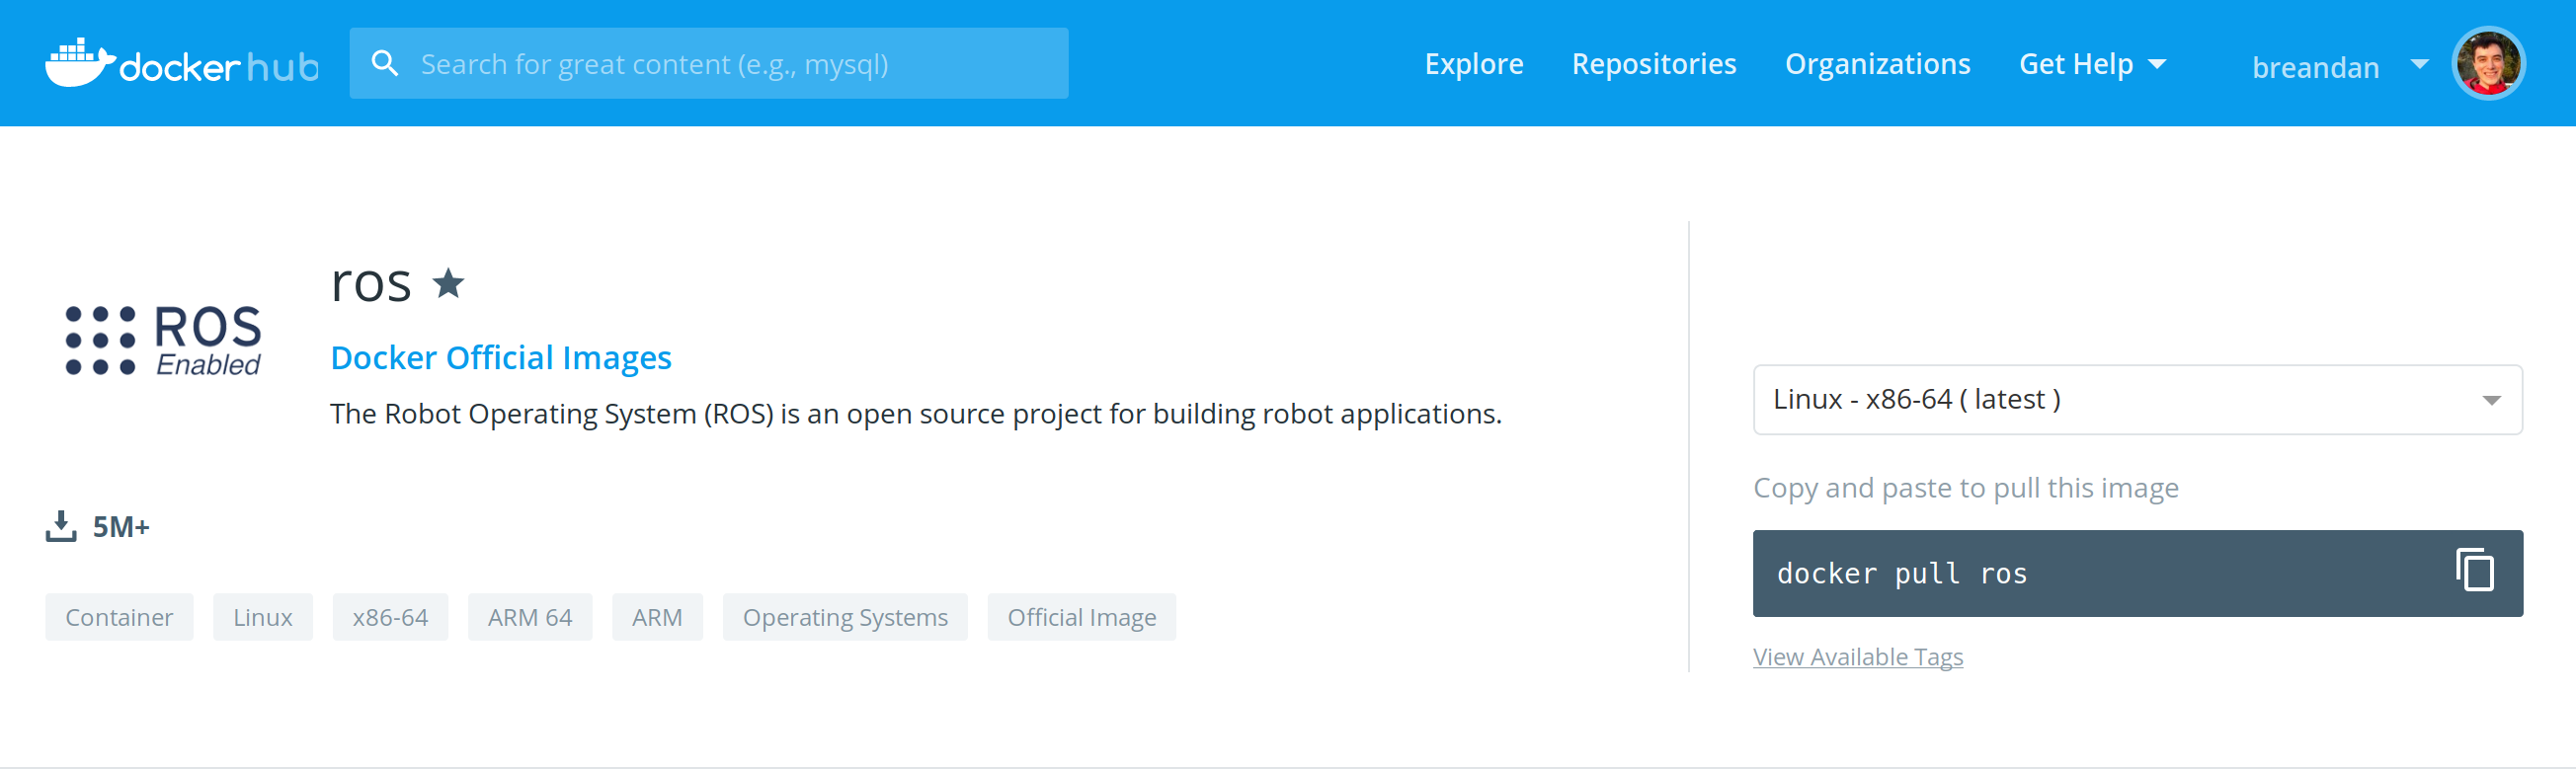
\includegraphics[width=\textwidth]{../figures/ros_docker_images.png}
\end{centering}

\subsection{\href{https://blog.hypriot.com/}{Hypriot}}\label{subsec:hypriot}

Hypriot, a base OS for RPi and other ARM devices, includes support for Docker straight out of the box. Hypriot is a lightweight Raspbian-based Linux distribution which \href{https://github.com/hypriot/image-builder-rpi}{builds} from the latest Raspberry Pi kernels and Raspbian releases.

\subsection{\href{https://www.piwheels.org/}{PiWheels}}

Not all Python packages (especially if they wrap a native library) can be run on all platforms. One might be tempted to build some package from its sources (and in rare cases, they might need to do so). But there is a good chance the package has already been compiled for Raspberry Pi on PiWheels. By using the following command (either in a \inline{Dockerfile} or via the CLI), various Python packages may be installed, e.g. \inline{opencv-python}:
%
\begin{rpilisting}
~$ pip install opencv-python --index-url https://www.piwheels.org/simple
\end{rpilisting}

\subsection{\href{https://hub.docker.com/}{Docker Hub}}\label{subsec:docker_hub}

Docker Hub is the central repository for Docker Images. Unless a separate registry has been configured, whenever users pull a Docker image tag, it will first query the Docker Hub for a matching image. The Docker Hub can be used to upload Docker images, and configure automated builds from GitHub (with a two hour build timeout). Docker Hub does not support layer caching of any kind, so the build will always take a fixed amount of time.\vspace{10pt}
%
\begin{centering}
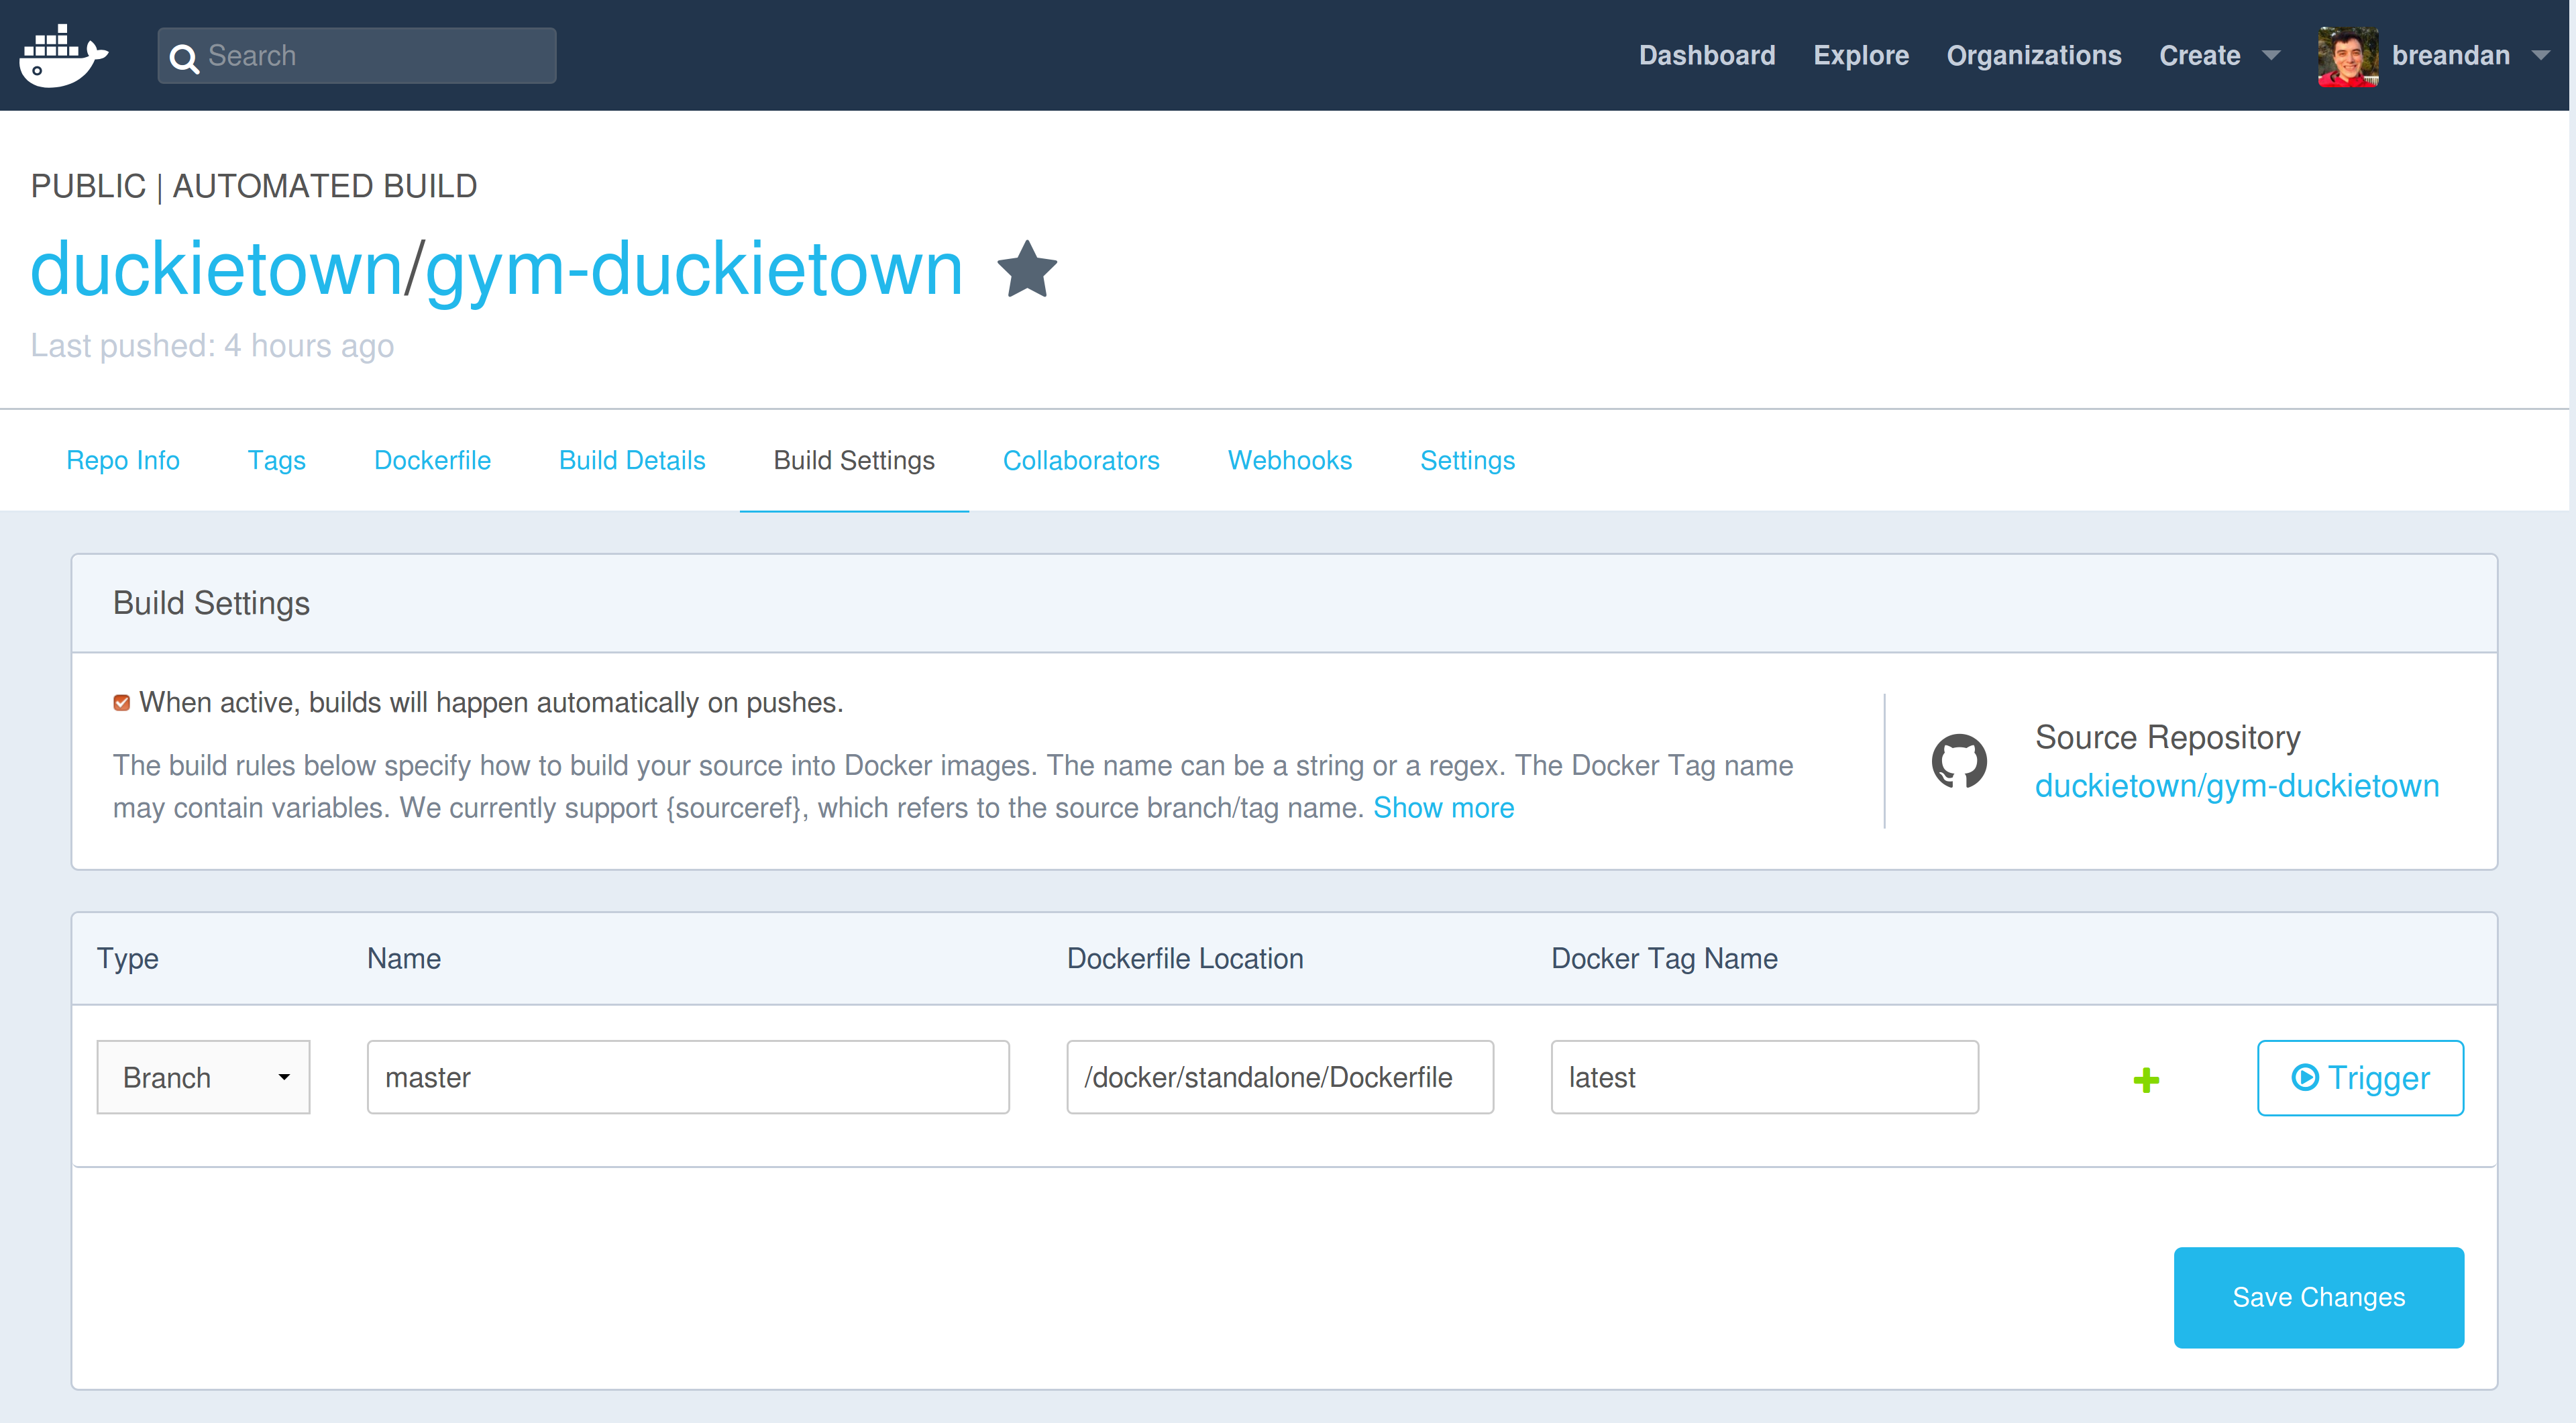
\includegraphics[width=\textwidth]{../figures/docker_hub_autobuild.png}
\end{centering}
%
Docker Hub auto-builds support linking a \inline{Dockerfile} in a GitHub repository, and whenever that \inline{Dockerfile} changes, the Docker image will be updated.

The Docker Hub also has features for configuring repository links and build triggers. These will automatically rebuild downstream Docker images whenever some event occurs.\vspace{10pt}
%
\begin{centering}
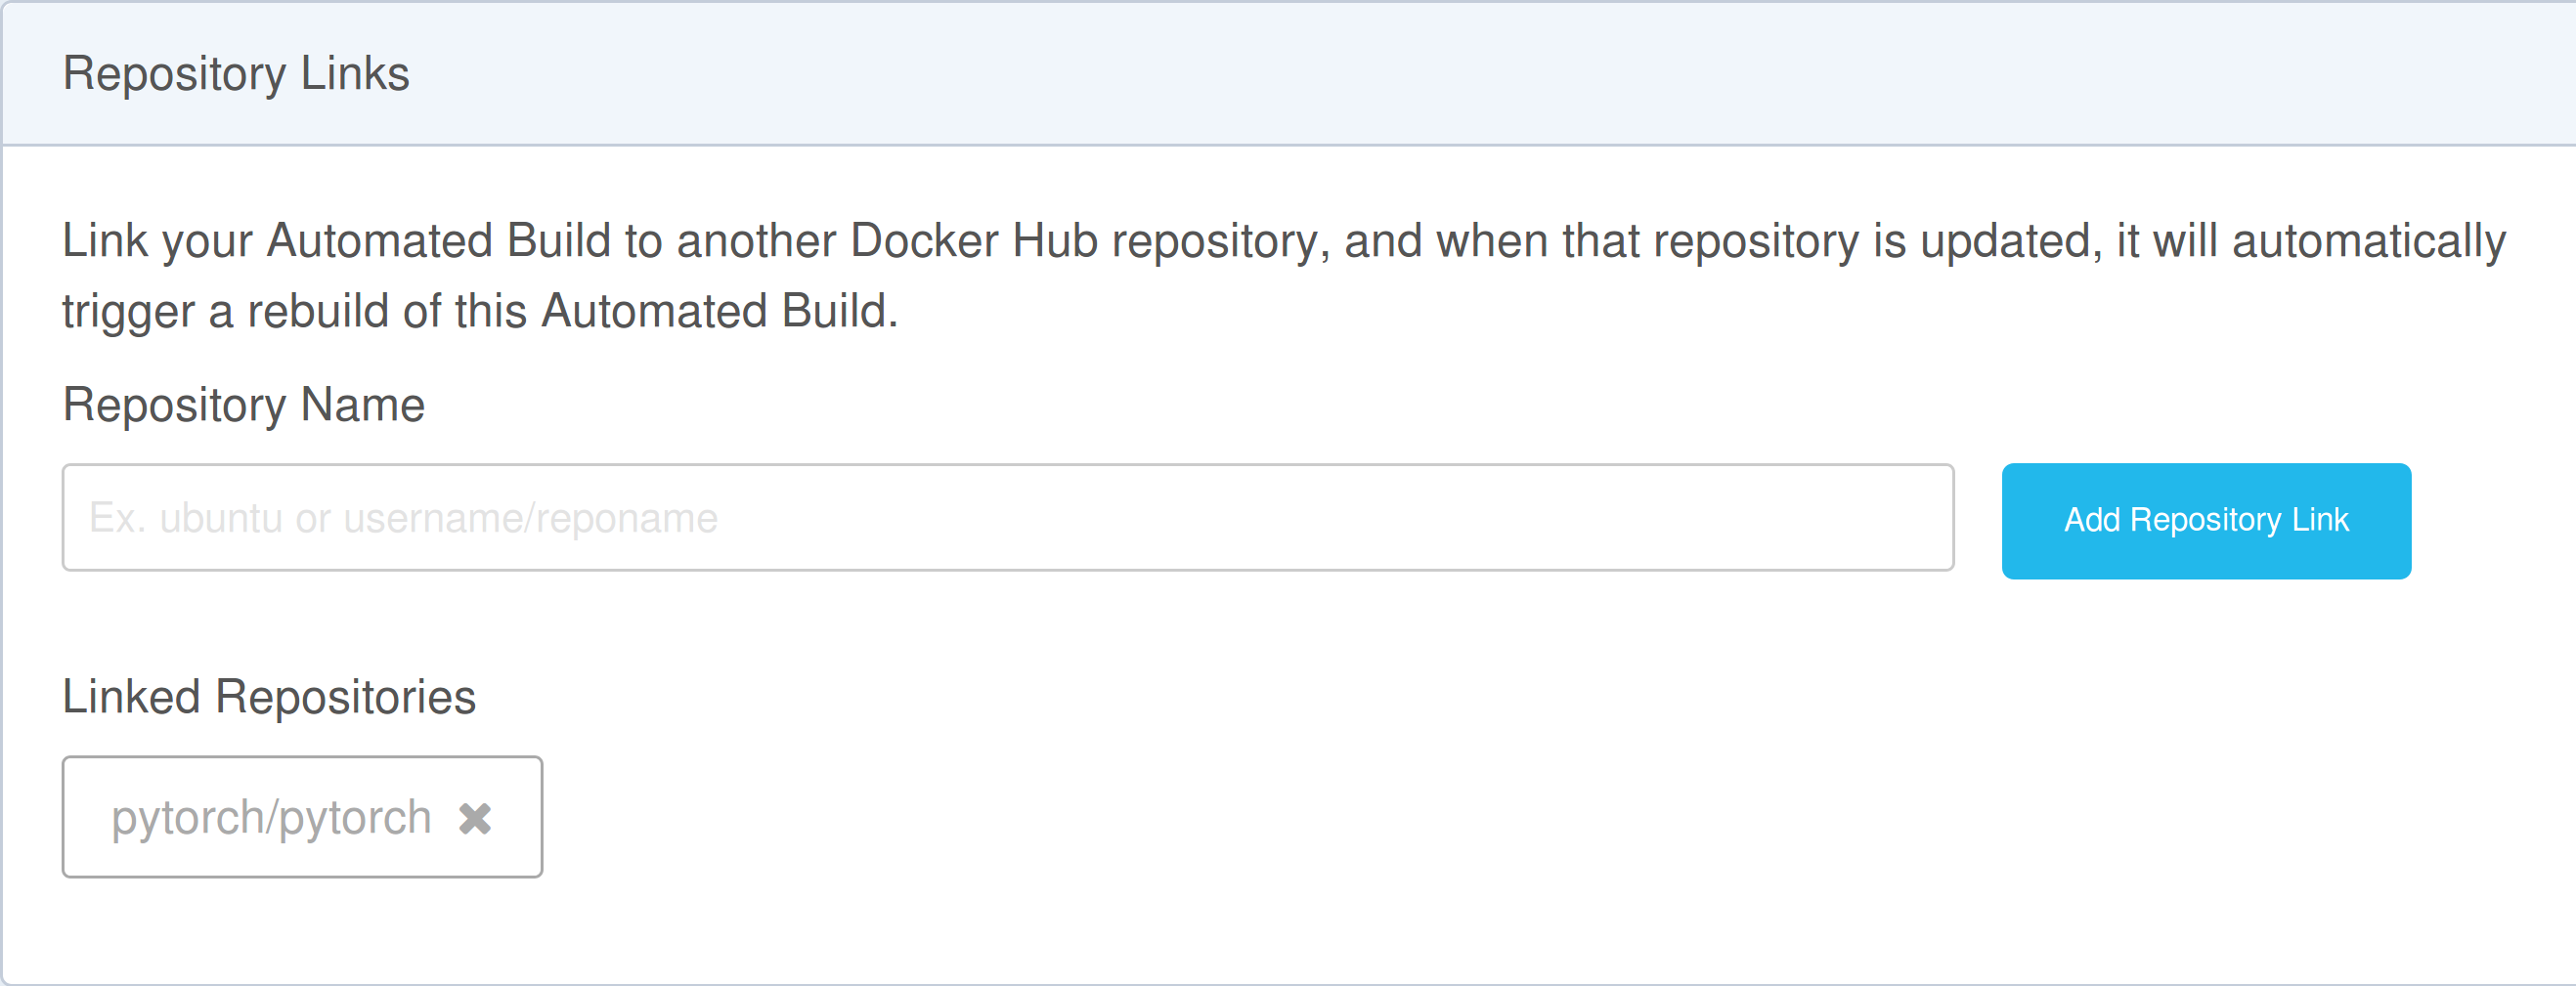
\includegraphics[width=\textwidth]{../figures/docker_hub_repo_links.png}
\end{centering}
%
Repository links allow support chaining builds together across Docker Hub repositories. Whenever a linked repository is updated, the dependent image will be rebuilt.

\subsection{\href{https://cloud.docker.com/}{Docker Cloud}}

Docker Cloud is a Docker registry which is fully integrated with the Docker Hub. Builds are automatically published from Docker Cloud to Docker Hub. Notifications for email and Slack, as well as longer build timeouts (up to 4-hours) are supported. Docker Cloud also supports more advanced build options than Docker Hub, such as a configurable build context and cache settings.\\

\begin{centering}
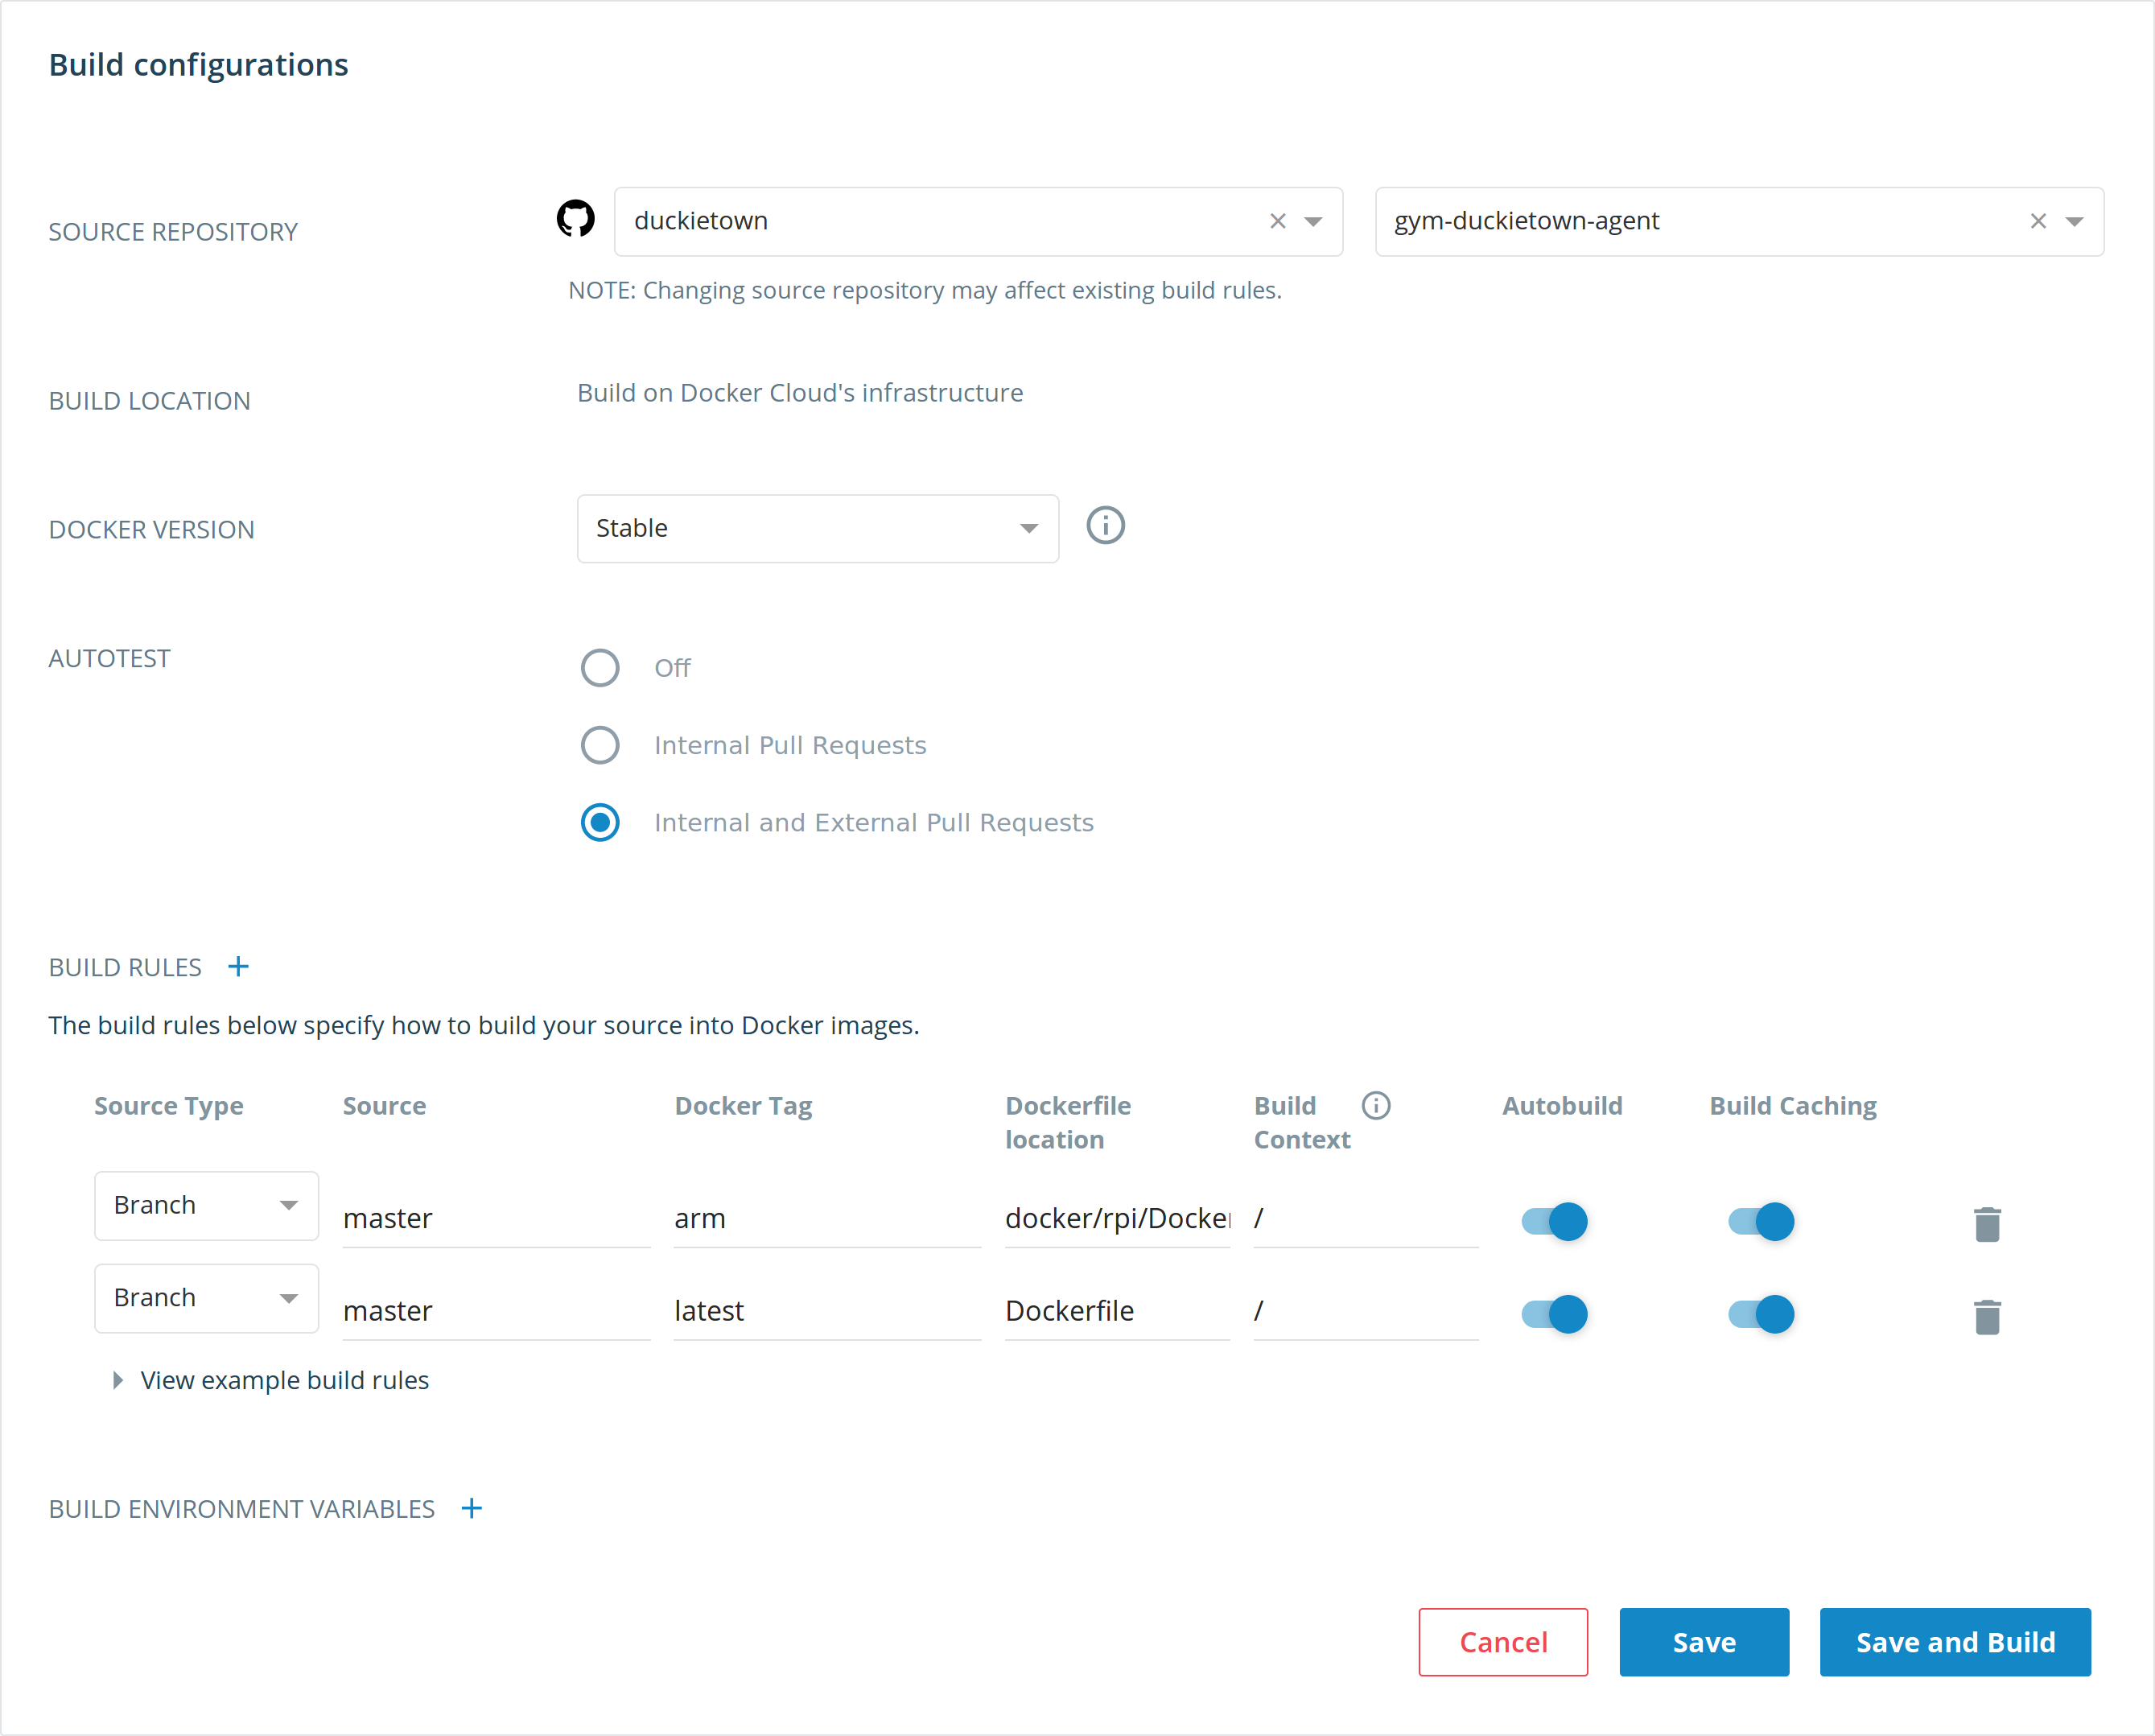
\includegraphics[width=\textwidth]{../figures/docker_cloud.png}
\end{centering}


\end{document}